%!TEX root = main.tex
\subsection{Simulation Study: OLS versus 2SLS Example}
\todo[inline]{Clean up the prose here.}
For simplicity, three instruments so the moments exist \citep{Phillips1980}. 
In other settings we could look at trimmed MSE or MAD.
Sample of $i = 1, \hdots, N$ observations from the following DGP 
\begin{eqnarray}
	y_i &=& 0.5 x_i + \epsilon_i\\
	x_i &=& \pi(z_{1i} + z_{2i} + z_{3i}) + v_i
\end{eqnarray}
where $(\epsilon_i, v_i, z_{1i}, z_{2i}, z_{3i}) \sim \mbox{ iid } N(0, \mathcal{S})$ and
\begin{equation}
	\mathcal{S} = \left[ \begin{array}
		{ccccc} 
		1 & \rho \sqrt{1-\pi^2}& 0 & 0 & 0\\
		\rho\sqrt{1-\pi^2} & 1 - \pi^2 & 0 & 0 & 0\\
		0 & 0 & 1/3 & 0 & 0\\
		0 & 0 & 0 & 1/3 & 0 \\
		0 & 0 & 0 & 0 & 1/3
	\end{array}\right]
\end{equation}
where $\pi = Corr(x_i, z_{1i} + z_{2i} + z_{3i})$ and $\rho = Corr(\epsilon_i, v_i)$ since the variance of $x$ is fixed at one.
This design satisfies the conditions of Assumption \ref{assump:OLSvsIV}.
Goal is to estimate $\beta$ which in this case equals 0.5.
Vary $N, \rho$, and $\pi$.
Following the formulas from Sections \ref{sec:OLSvsIVlowlevel} and \ref{sec:FMSCforOLSvsIV} compare FMSC against OLS, 2SLS, and DHW pre-test estimators at the standard significance levels of 90 and 95\% in terms of estimator RMSE.

\begin{figure}
\centering
	% Created by tikzDevice version 0.7.0 on 2014-06-30 20:14:00
% !TEX encoding = UTF-8 Unicode
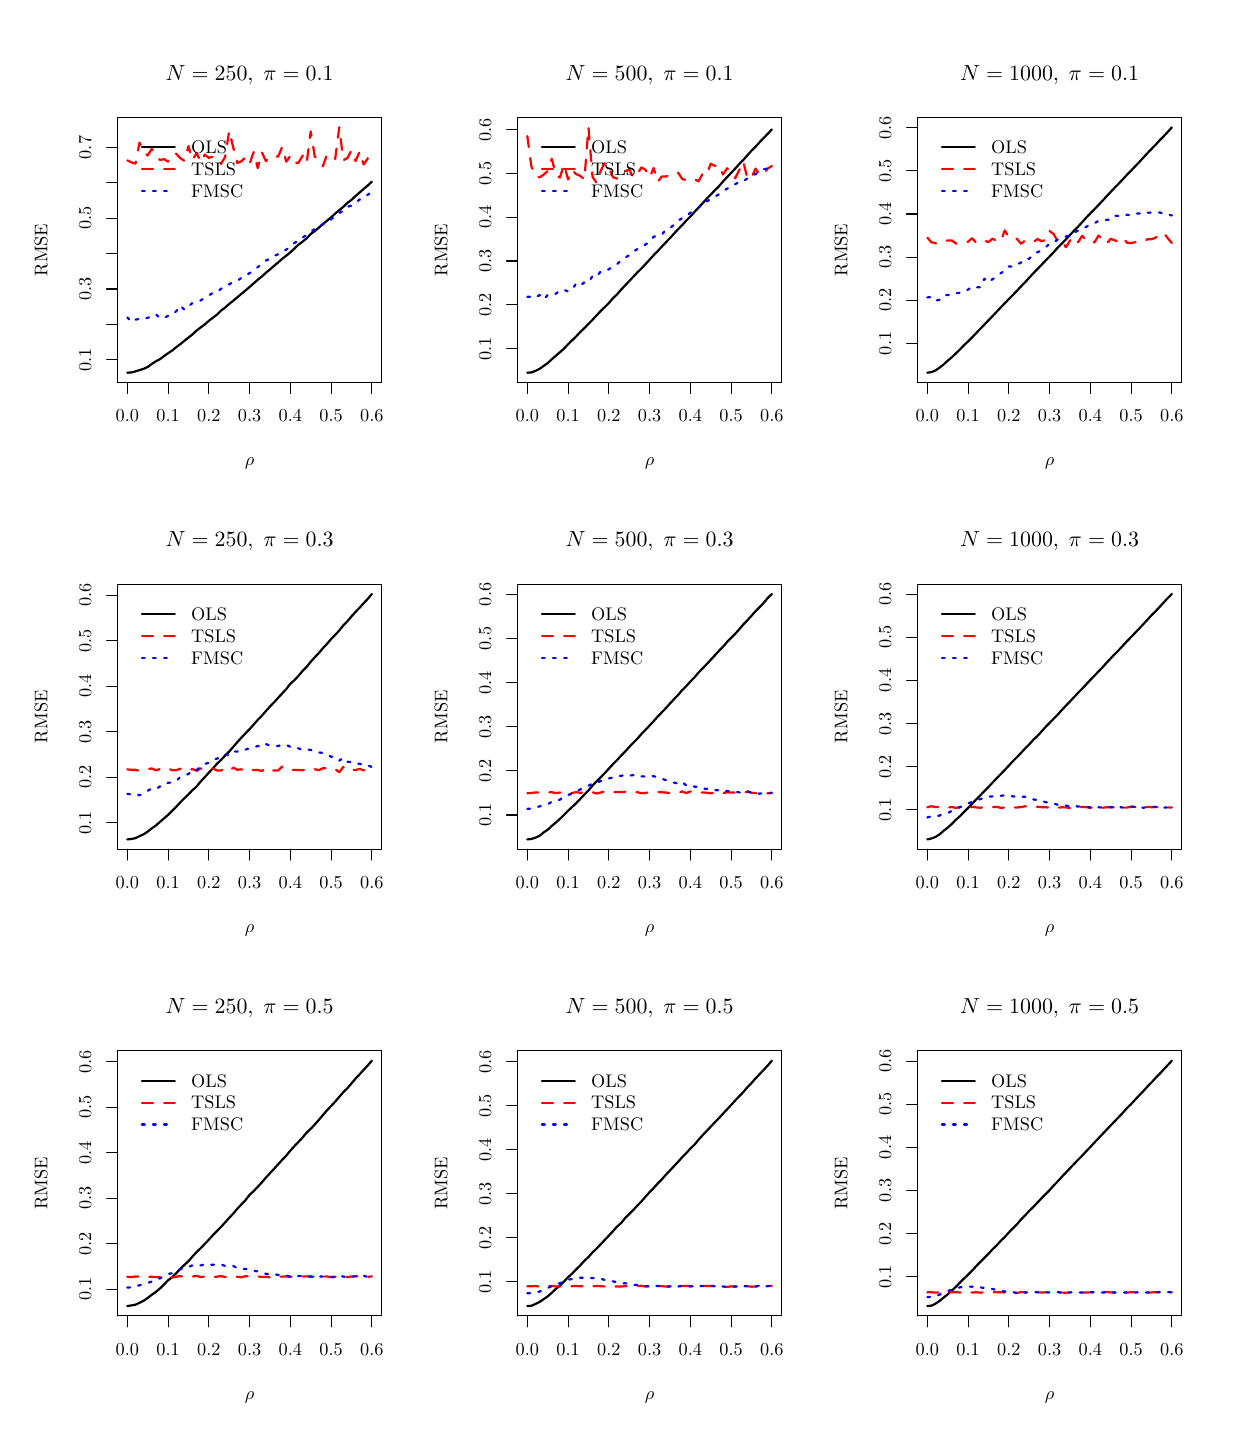
\begin{tikzpicture}[x=1pt,y=1pt]
\definecolor[named]{fillColor}{rgb}{1.00,1.00,1.00}
\path[use as bounding box,fill=fillColor,fill opacity=0.00] (0,0) rectangle (433.62,505.89);
\begin{scope}
\path[clip] ( 32.47,377.65) rectangle (127.91,473.42);
\definecolor[named]{drawColor}{rgb}{0.00,0.00,0.00}

\path[draw=drawColor,line width= 0.8pt,line join=round,line cap=round] ( 36.01,381.20) --
	( 37.48,381.31) --
	( 38.95,381.68) --
	( 40.42,382.15) --
	( 41.90,382.62) --
	( 43.37,383.28) --
	( 44.84,384.36) --
	( 46.32,385.32) --
	( 47.79,386.08) --
	( 49.26,387.20) --
	( 50.73,388.24) --
	( 52.21,389.21) --
	( 53.68,390.44) --
	( 55.15,391.53) --
	( 56.63,392.74) --
	( 58.10,393.92) --
	( 59.57,395.06) --
	( 61.04,396.45) --
	( 62.52,397.56) --
	( 63.99,398.65) --
	( 65.46,399.95) --
	( 66.93,401.10) --
	( 68.41,402.21) --
	( 69.88,403.65) --
	( 71.35,404.77) --
	( 72.83,406.06) --
	( 74.30,407.22) --
	( 75.77,408.48) --
	( 77.24,409.71) --
	( 78.72,410.94) --
	( 80.19,412.19) --
	( 81.66,413.47) --
	( 83.14,414.81) --
	( 84.61,415.96) --
	( 86.08,417.32) --
	( 87.55,418.51) --
	( 89.03,419.82) --
	( 90.50,421.04) --
	( 91.97,422.37) --
	( 93.44,423.48) --
	( 94.92,424.71) --
	( 96.39,426.08) --
	( 97.86,427.47) --
	( 99.34,428.57) --
	(100.81,429.76) --
	(102.28,431.34) --
	(103.75,432.41) --
	(105.23,433.63) --
	(106.70,434.96) --
	(108.17,436.12) --
	(109.65,437.35) --
	(111.12,438.70) --
	(112.59,439.94) --
	(114.06,441.14) --
	(115.54,442.56) --
	(117.01,443.66) --
	(118.48,445.05) --
	(119.95,446.32) --
	(121.43,447.63) --
	(122.90,448.86) --
	(124.37,450.23);
\end{scope}
\begin{scope}
\path[clip] (  0.00,  0.00) rectangle (433.62,505.89);
\definecolor[named]{drawColor}{rgb}{0.00,0.00,0.00}

\path[draw=drawColor,line width= 0.4pt,line join=round,line cap=round] ( 36.01,377.65) -- (124.37,377.65);

\path[draw=drawColor,line width= 0.4pt,line join=round,line cap=round] ( 36.01,377.65) -- ( 36.01,373.69);

\path[draw=drawColor,line width= 0.4pt,line join=round,line cap=round] ( 50.73,377.65) -- ( 50.73,373.69);

\path[draw=drawColor,line width= 0.4pt,line join=round,line cap=round] ( 65.46,377.65) -- ( 65.46,373.69);

\path[draw=drawColor,line width= 0.4pt,line join=round,line cap=round] ( 80.19,377.65) -- ( 80.19,373.69);

\path[draw=drawColor,line width= 0.4pt,line join=round,line cap=round] ( 94.92,377.65) -- ( 94.92,373.69);

\path[draw=drawColor,line width= 0.4pt,line join=round,line cap=round] (109.65,377.65) -- (109.65,373.69);

\path[draw=drawColor,line width= 0.4pt,line join=round,line cap=round] (124.37,377.65) -- (124.37,373.69);

\node[text=drawColor,anchor=base,inner sep=0pt, outer sep=0pt, scale=  0.66] at ( 36.01,363.40) {0.0};

\node[text=drawColor,anchor=base,inner sep=0pt, outer sep=0pt, scale=  0.66] at ( 50.73,363.40) {0.1};

\node[text=drawColor,anchor=base,inner sep=0pt, outer sep=0pt, scale=  0.66] at ( 65.46,363.40) {0.2};

\node[text=drawColor,anchor=base,inner sep=0pt, outer sep=0pt, scale=  0.66] at ( 80.19,363.40) {0.3};

\node[text=drawColor,anchor=base,inner sep=0pt, outer sep=0pt, scale=  0.66] at ( 94.92,363.40) {0.4};

\node[text=drawColor,anchor=base,inner sep=0pt, outer sep=0pt, scale=  0.66] at (109.65,363.40) {0.5};

\node[text=drawColor,anchor=base,inner sep=0pt, outer sep=0pt, scale=  0.66] at (124.37,363.40) {0.6};

\path[draw=drawColor,line width= 0.4pt,line join=round,line cap=round] ( 32.47,385.90) -- ( 32.47,462.60);

\path[draw=drawColor,line width= 0.4pt,line join=round,line cap=round] ( 32.47,385.90) -- ( 28.51,385.90);

\path[draw=drawColor,line width= 0.4pt,line join=round,line cap=round] ( 32.47,398.68) -- ( 28.51,398.68);

\path[draw=drawColor,line width= 0.4pt,line join=round,line cap=round] ( 32.47,411.46) -- ( 28.51,411.46);

\path[draw=drawColor,line width= 0.4pt,line join=round,line cap=round] ( 32.47,424.25) -- ( 28.51,424.25);

\path[draw=drawColor,line width= 0.4pt,line join=round,line cap=round] ( 32.47,437.03) -- ( 28.51,437.03);

\path[draw=drawColor,line width= 0.4pt,line join=round,line cap=round] ( 32.47,449.81) -- ( 28.51,449.81);

\path[draw=drawColor,line width= 0.4pt,line join=round,line cap=round] ( 32.47,462.60) -- ( 28.51,462.60);

\node[text=drawColor,rotate= 90.00,anchor=base,inner sep=0pt, outer sep=0pt, scale=  0.66] at ( 22.97,385.90) {0.1};

\node[text=drawColor,rotate= 90.00,anchor=base,inner sep=0pt, outer sep=0pt, scale=  0.66] at ( 22.97,411.46) {0.3};

\node[text=drawColor,rotate= 90.00,anchor=base,inner sep=0pt, outer sep=0pt, scale=  0.66] at ( 22.97,437.03) {0.5};

\node[text=drawColor,rotate= 90.00,anchor=base,inner sep=0pt, outer sep=0pt, scale=  0.66] at ( 22.97,462.60) {0.7};

\path[draw=drawColor,line width= 0.4pt,line join=round,line cap=round] ( 32.47,377.65) --
	(127.91,377.65) --
	(127.91,473.42) --
	( 32.47,473.42) --
	( 32.47,377.65);
\end{scope}
\begin{scope}
\path[clip] (  0.00,337.26) rectangle (144.54,505.89);
\definecolor[named]{drawColor}{rgb}{0.00,0.00,0.00}

\node[text=drawColor,anchor=base,inner sep=0pt, outer sep=0pt, scale=  0.79] at ( 80.19,486.92) {\bfseries $N=250, \;\pi=0.1$};

\node[text=drawColor,anchor=base,inner sep=0pt, outer sep=0pt, scale=  0.66] at ( 80.19,347.56) {$\rho$};

\node[text=drawColor,rotate= 90.00,anchor=base,inner sep=0pt, outer sep=0pt, scale=  0.66] at (  7.13,425.53) {RMSE};
\end{scope}
\begin{scope}
\path[clip] ( 32.47,377.65) rectangle (127.91,473.42);
\definecolor[named]{drawColor}{rgb}{1.00,0.00,0.00}

\path[draw=drawColor,line width= 0.8pt,dash pattern=on 4pt off 4pt ,line join=round,line cap=round] ( 36.01,457.95) --
	( 37.48,457.23) --
	( 38.95,456.75) --
	( 40.42,464.40) --
	( 41.90,460.96) --
	( 43.37,459.70) --
	( 44.84,462.07) --
	( 46.32,460.20) --
	( 47.79,458.06) --
	( 49.26,458.38) --
	( 50.73,457.46) --
	( 52.21,460.09) --
	( 53.68,460.32) --
	( 55.15,458.72) --
	( 56.63,457.75) --
	( 58.10,463.08) --
	( 59.57,458.02) --
	( 61.04,460.66) --
	( 62.52,457.29) --
	( 63.99,460.03) --
	( 65.46,458.82) --
	( 66.93,459.30) --
	( 68.41,459.00) --
	( 69.88,456.67) --
	( 71.35,459.20) --
	( 72.83,468.61) --
	( 74.30,462.50) --
	( 75.77,456.99) --
	( 77.24,457.61) --
	( 78.72,459.03) --
	( 80.19,456.60) --
	( 81.66,460.94) --
	( 83.14,455.16) --
	( 84.61,460.90) --
	( 86.08,457.66) --
	( 87.55,459.05) --
	( 89.03,459.65) --
	( 90.50,459.28) --
	( 91.97,462.79) --
	( 93.44,457.46) --
	( 94.92,459.60) --
	( 96.39,457.07) --
	( 97.86,457.06) --
	( 99.34,459.61) --
	(100.81,456.94) --
	(102.28,468.40) --
	(103.75,459.28) --
	(105.23,458.38) --
	(106.70,455.83) --
	(108.17,460.12) --
	(109.65,459.69) --
	(111.12,458.49) --
	(112.59,469.87) --
	(114.06,457.98) --
	(115.54,458.80) --
	(117.01,461.53) --
	(118.48,457.65) --
	(119.95,461.08) --
	(121.43,456.45) --
	(122.90,458.67) --
	(124.37,458.90);
\definecolor[named]{drawColor}{rgb}{0.00,0.00,1.00}

\path[draw=drawColor,line width= 0.8pt,dash pattern=on 1pt off 3pt ,line join=round,line cap=round] ( 36.01,401.23) --
	( 37.48,399.51) --
	( 38.95,400.37) --
	( 40.42,400.68) --
	( 41.90,400.58) --
	( 43.37,401.06) --
	( 44.84,401.50) --
	( 46.32,402.38) --
	( 47.79,400.86) --
	( 49.26,401.05) --
	( 50.73,401.72) --
	( 52.21,402.10) --
	( 53.68,403.44) --
	( 55.15,405.52) --
	( 56.63,403.92) --
	( 58.10,405.22) --
	( 59.57,406.39) --
	( 61.04,406.79) --
	( 62.52,407.29) --
	( 63.99,408.38) --
	( 65.46,409.16) --
	( 66.93,410.04) --
	( 68.41,410.28) --
	( 69.88,411.56) --
	( 71.35,412.21) --
	( 72.83,413.16) --
	( 74.30,414.05) --
	( 75.77,414.43) --
	( 77.24,415.48) --
	( 78.72,416.45) --
	( 80.19,417.20) --
	( 81.66,418.15) --
	( 83.14,419.36) --
	( 84.61,420.47) --
	( 86.08,421.71) --
	( 87.55,422.44) --
	( 89.03,423.38) --
	( 90.50,424.02) --
	( 91.97,425.01) --
	( 93.44,425.67) --
	( 94.92,426.78) --
	( 96.39,428.09) --
	( 97.86,429.00) --
	( 99.34,430.06) --
	(100.81,430.97) --
	(102.28,432.17) --
	(103.75,433.15) --
	(105.23,434.11) --
	(106.70,434.83) --
	(108.17,436.14) --
	(109.65,436.56) --
	(111.12,437.98) --
	(112.59,438.93) --
	(114.06,439.74) --
	(115.54,441.18) --
	(117.01,441.57) --
	(118.48,442.76) --
	(119.95,443.77) --
	(121.43,444.41) --
	(122.90,445.51) --
	(124.37,446.59);
\definecolor[named]{drawColor}{rgb}{0.00,0.00,0.00}

\path[draw=drawColor,line width= 0.8pt,line join=round,line cap=round] ( 41.28,462.63) -- ( 53.16,462.63);
\definecolor[named]{drawColor}{rgb}{1.00,0.00,0.00}

\path[draw=drawColor,line width= 0.8pt,dash pattern=on 4pt off 4pt ,line join=round,line cap=round] ( 41.28,454.71) -- ( 53.16,454.71);
\definecolor[named]{drawColor}{rgb}{0.00,0.00,1.00}

\path[draw=drawColor,line width= 0.8pt,dash pattern=on 1pt off 3pt ,line join=round,line cap=round] ( 41.28,446.79) -- ( 53.16,446.79);
\definecolor[named]{drawColor}{rgb}{0.00,0.00,0.00}

\node[text=drawColor,anchor=base west,inner sep=0pt, outer sep=0pt, scale=  0.66] at ( 59.10,460.35) {OLS};

\node[text=drawColor,anchor=base west,inner sep=0pt, outer sep=0pt, scale=  0.66] at ( 59.10,452.43) {TSLS};

\node[text=drawColor,anchor=base west,inner sep=0pt, outer sep=0pt, scale=  0.66] at ( 59.10,444.51) {FMSC};
\end{scope}
\begin{scope}
\path[clip] (177.01,377.65) rectangle (272.45,473.42);
\definecolor[named]{drawColor}{rgb}{0.00,0.00,0.00}

\path[draw=drawColor,line width= 0.8pt,line join=round,line cap=round] (180.55,381.20) --
	(182.02,381.31) --
	(183.49,381.86) --
	(184.96,382.60) --
	(186.44,383.64) --
	(187.91,384.69) --
	(189.38,386.05) --
	(190.86,387.35) --
	(192.33,388.61) --
	(193.80,389.91) --
	(195.27,391.49) --
	(196.75,392.93) --
	(198.22,394.33) --
	(199.69,395.94) --
	(201.17,397.31) --
	(202.64,398.85) --
	(204.11,400.33) --
	(205.58,401.90) --
	(207.06,403.51) --
	(208.53,404.92) --
	(210.00,406.39) --
	(211.47,408.09) --
	(212.95,409.49) --
	(214.42,411.19) --
	(215.89,412.76) --
	(217.37,414.30) --
	(218.84,415.87) --
	(220.31,417.45) --
	(221.78,418.87) --
	(223.26,420.47) --
	(224.73,422.05) --
	(226.20,423.70) --
	(227.68,425.16) --
	(229.15,426.77) --
	(230.62,428.32) --
	(232.09,429.84) --
	(233.57,431.48) --
	(235.04,433.06) --
	(236.51,434.55) --
	(237.98,436.16) --
	(239.46,437.64) --
	(240.93,439.28) --
	(242.40,440.84) --
	(243.88,442.42) --
	(245.35,444.06) --
	(246.82,445.54) --
	(248.29,447.10) --
	(249.77,448.55) --
	(251.24,450.29) --
	(252.71,451.85) --
	(254.19,453.41) --
	(255.66,454.98) --
	(257.13,456.61) --
	(258.60,458.10) --
	(260.08,459.78) --
	(261.55,461.44) --
	(263.02,462.86) --
	(264.50,464.51) --
	(265.97,466.07) --
	(267.44,467.55) --
	(268.91,469.15);
\end{scope}
\begin{scope}
\path[clip] (  0.00,  0.00) rectangle (433.62,505.89);
\definecolor[named]{drawColor}{rgb}{0.00,0.00,0.00}

\path[draw=drawColor,line width= 0.4pt,line join=round,line cap=round] (180.55,377.65) -- (268.91,377.65);

\path[draw=drawColor,line width= 0.4pt,line join=round,line cap=round] (180.55,377.65) -- (180.55,373.69);

\path[draw=drawColor,line width= 0.4pt,line join=round,line cap=round] (195.27,377.65) -- (195.27,373.69);

\path[draw=drawColor,line width= 0.4pt,line join=round,line cap=round] (210.00,377.65) -- (210.00,373.69);

\path[draw=drawColor,line width= 0.4pt,line join=round,line cap=round] (224.73,377.65) -- (224.73,373.69);

\path[draw=drawColor,line width= 0.4pt,line join=round,line cap=round] (239.46,377.65) -- (239.46,373.69);

\path[draw=drawColor,line width= 0.4pt,line join=round,line cap=round] (254.19,377.65) -- (254.19,373.69);

\path[draw=drawColor,line width= 0.4pt,line join=round,line cap=round] (268.91,377.65) -- (268.91,373.69);

\node[text=drawColor,anchor=base,inner sep=0pt, outer sep=0pt, scale=  0.66] at (180.55,363.40) {0.0};

\node[text=drawColor,anchor=base,inner sep=0pt, outer sep=0pt, scale=  0.66] at (195.27,363.40) {0.1};

\node[text=drawColor,anchor=base,inner sep=0pt, outer sep=0pt, scale=  0.66] at (210.00,363.40) {0.2};

\node[text=drawColor,anchor=base,inner sep=0pt, outer sep=0pt, scale=  0.66] at (224.73,363.40) {0.3};

\node[text=drawColor,anchor=base,inner sep=0pt, outer sep=0pt, scale=  0.66] at (239.46,363.40) {0.4};

\node[text=drawColor,anchor=base,inner sep=0pt, outer sep=0pt, scale=  0.66] at (254.19,363.40) {0.5};

\node[text=drawColor,anchor=base,inner sep=0pt, outer sep=0pt, scale=  0.66] at (268.91,363.40) {0.6};

\path[draw=drawColor,line width= 0.4pt,line join=round,line cap=round] (177.01,389.93) -- (177.01,469.01);

\path[draw=drawColor,line width= 0.4pt,line join=round,line cap=round] (177.01,389.93) -- (173.05,389.93);

\path[draw=drawColor,line width= 0.4pt,line join=round,line cap=round] (177.01,405.74) -- (173.05,405.74);

\path[draw=drawColor,line width= 0.4pt,line join=round,line cap=round] (177.01,421.56) -- (173.05,421.56);

\path[draw=drawColor,line width= 0.4pt,line join=round,line cap=round] (177.01,437.38) -- (173.05,437.38);

\path[draw=drawColor,line width= 0.4pt,line join=round,line cap=round] (177.01,453.19) -- (173.05,453.19);

\path[draw=drawColor,line width= 0.4pt,line join=round,line cap=round] (177.01,469.01) -- (173.05,469.01);

\node[text=drawColor,rotate= 90.00,anchor=base,inner sep=0pt, outer sep=0pt, scale=  0.66] at (167.51,389.93) {0.1};

\node[text=drawColor,rotate= 90.00,anchor=base,inner sep=0pt, outer sep=0pt, scale=  0.66] at (167.51,405.74) {0.2};

\node[text=drawColor,rotate= 90.00,anchor=base,inner sep=0pt, outer sep=0pt, scale=  0.66] at (167.51,421.56) {0.3};

\node[text=drawColor,rotate= 90.00,anchor=base,inner sep=0pt, outer sep=0pt, scale=  0.66] at (167.51,437.38) {0.4};

\node[text=drawColor,rotate= 90.00,anchor=base,inner sep=0pt, outer sep=0pt, scale=  0.66] at (167.51,453.19) {0.5};

\node[text=drawColor,rotate= 90.00,anchor=base,inner sep=0pt, outer sep=0pt, scale=  0.66] at (167.51,469.01) {0.6};

\path[draw=drawColor,line width= 0.4pt,line join=round,line cap=round] (177.01,377.65) --
	(272.45,377.65) --
	(272.45,473.42) --
	(177.01,473.42) --
	(177.01,377.65);
\end{scope}
\begin{scope}
\path[clip] (144.54,337.26) rectangle (289.08,505.89);
\definecolor[named]{drawColor}{rgb}{0.00,0.00,0.00}

\node[text=drawColor,anchor=base,inner sep=0pt, outer sep=0pt, scale=  0.79] at (224.73,486.92) {\bfseries $N=500, \;\pi=0.1$};

\node[text=drawColor,anchor=base,inner sep=0pt, outer sep=0pt, scale=  0.66] at (224.73,347.56) {$\rho$};

\node[text=drawColor,rotate= 90.00,anchor=base,inner sep=0pt, outer sep=0pt, scale=  0.66] at (151.67,425.53) {RMSE};
\end{scope}
\begin{scope}
\path[clip] (177.01,377.65) rectangle (272.45,473.42);
\definecolor[named]{drawColor}{rgb}{1.00,0.00,0.00}

\path[draw=drawColor,line width= 0.8pt,dash pattern=on 4pt off 4pt ,line join=round,line cap=round] (180.55,466.72) --
	(182.02,455.74) --
	(183.49,452.28) --
	(184.96,451.80) --
	(186.44,452.78) --
	(187.91,454.08) --
	(189.38,458.54) --
	(190.86,452.70) --
	(192.33,451.73) --
	(193.80,456.48) --
	(195.27,451.04) --
	(196.75,454.48) --
	(198.22,452.92) --
	(199.69,452.35) --
	(201.17,450.95) --
	(202.64,469.87) --
	(204.11,451.98) --
	(205.58,449.82) --
	(207.06,454.09) --
	(208.53,457.15) --
	(210.00,455.29) --
	(211.47,451.89) --
	(212.95,451.34) --
	(214.42,453.57) --
	(215.89,454.06) --
	(217.37,454.59) --
	(218.84,451.70) --
	(220.31,453.03) --
	(221.78,455.41) --
	(223.26,454.53) --
	(224.73,451.76) --
	(226.20,455.17) --
	(227.68,450.17) --
	(229.15,452.12) --
	(230.62,452.05) --
	(232.09,452.77) --
	(233.57,452.63) --
	(235.04,453.52) --
	(236.51,451.22) --
	(237.98,450.77) --
	(239.46,451.21) --
	(240.93,451.13) --
	(242.40,450.37) --
	(243.88,453.05) --
	(245.35,452.60) --
	(246.82,456.72) --
	(248.29,455.97) --
	(249.77,456.22) --
	(251.24,452.84) --
	(252.71,455.06) --
	(254.19,454.01) --
	(255.66,451.46) --
	(257.13,454.41) --
	(258.60,457.49) --
	(260.08,451.34) --
	(261.55,451.78) --
	(263.02,454.96) --
	(264.50,452.70) --
	(265.97,453.02) --
	(267.44,455.04) --
	(268.91,455.88);
\definecolor[named]{drawColor}{rgb}{0.00,0.00,1.00}

\path[draw=drawColor,line width= 0.8pt,dash pattern=on 1pt off 3pt ,line join=round,line cap=round] (180.55,408.62) --
	(182.02,408.70) --
	(183.49,408.29) --
	(184.96,409.27) --
	(186.44,407.70) --
	(187.91,409.28) --
	(189.38,409.87) --
	(190.86,409.74) --
	(192.33,411.06) --
	(193.80,411.13) --
	(195.27,410.58) --
	(196.75,411.25) --
	(198.22,413.50) --
	(199.69,412.72) --
	(201.17,413.86) --
	(202.64,413.80) --
	(204.11,416.17) --
	(205.58,415.89) --
	(207.06,417.80) --
	(208.53,417.86) --
	(210.00,418.58) --
	(211.47,419.59) --
	(212.95,420.41) --
	(214.42,421.78) --
	(215.89,422.84) --
	(217.37,423.63) --
	(218.84,424.92) --
	(220.31,425.87) --
	(221.78,426.51) --
	(223.26,427.57) --
	(224.73,428.44) --
	(226.20,430.34) --
	(227.68,430.70) --
	(229.15,431.08) --
	(230.62,432.93) --
	(232.09,433.47) --
	(233.57,434.66) --
	(235.04,436.09) --
	(236.51,437.10) --
	(237.98,437.72) --
	(239.46,439.02) --
	(240.93,439.77) --
	(242.40,440.86) --
	(243.88,442.22) --
	(245.35,443.13) --
	(246.82,443.89) --
	(248.29,444.81) --
	(249.77,445.67) --
	(251.24,446.76) --
	(252.71,447.72) --
	(254.19,448.30) --
	(255.66,449.32) --
	(257.13,450.22) --
	(258.60,450.35) --
	(260.08,451.46) --
	(261.55,452.36) --
	(263.02,452.95) --
	(264.50,454.18) --
	(265.97,454.74) --
	(267.44,454.96) --
	(268.91,455.83);
\definecolor[named]{drawColor}{rgb}{0.00,0.00,0.00}

\path[draw=drawColor,line width= 0.8pt,line join=round,line cap=round] (185.82,462.63) -- (197.70,462.63);
\definecolor[named]{drawColor}{rgb}{1.00,0.00,0.00}

\path[draw=drawColor,line width= 0.8pt,dash pattern=on 4pt off 4pt ,line join=round,line cap=round] (185.82,454.71) -- (197.70,454.71);
\definecolor[named]{drawColor}{rgb}{0.00,0.00,1.00}

\path[draw=drawColor,line width= 0.8pt,dash pattern=on 1pt off 3pt ,line join=round,line cap=round] (185.82,446.79) -- (197.70,446.79);
\definecolor[named]{drawColor}{rgb}{0.00,0.00,0.00}

\node[text=drawColor,anchor=base west,inner sep=0pt, outer sep=0pt, scale=  0.66] at (203.64,460.35) {OLS};

\node[text=drawColor,anchor=base west,inner sep=0pt, outer sep=0pt, scale=  0.66] at (203.64,452.43) {TSLS};

\node[text=drawColor,anchor=base west,inner sep=0pt, outer sep=0pt, scale=  0.66] at (203.64,444.51) {FMSC};
\end{scope}
\begin{scope}
\path[clip] (321.55,377.65) rectangle (416.99,473.42);
\definecolor[named]{drawColor}{rgb}{0.00,0.00,0.00}

\path[draw=drawColor,line width= 0.8pt,line join=round,line cap=round] (325.09,381.20) --
	(326.56,381.41) --
	(328.03,382.02) --
	(329.50,383.03) --
	(330.98,384.18) --
	(332.45,385.54) --
	(333.92,386.78) --
	(335.40,388.19) --
	(336.87,389.60) --
	(338.34,391.14) --
	(339.81,392.51) --
	(341.29,394.00) --
	(342.76,395.54) --
	(344.23,397.07) --
	(345.71,398.61) --
	(347.18,400.14) --
	(348.65,401.63) --
	(350.12,403.22) --
	(351.60,404.78) --
	(353.07,406.31) --
	(354.54,407.83) --
	(356.01,409.31) --
	(357.49,410.83) --
	(358.96,412.41) --
	(360.43,413.91) --
	(361.91,415.52) --
	(363.38,417.12) --
	(364.85,418.65) --
	(366.32,420.15) --
	(367.80,421.71) --
	(369.27,423.21) --
	(370.74,424.75) --
	(372.22,426.41) --
	(373.69,427.86) --
	(375.16,429.38) --
	(376.63,430.99) --
	(378.11,432.53) --
	(379.58,434.01) --
	(381.05,435.61) --
	(382.52,437.26) --
	(384.00,438.78) --
	(385.47,440.27) --
	(386.94,441.81) --
	(388.42,443.37) --
	(389.89,444.98) --
	(391.36,446.54) --
	(392.83,448.11) --
	(394.31,449.61) --
	(395.78,451.15) --
	(397.25,452.74) --
	(398.73,454.23) --
	(400.20,455.80) --
	(401.67,457.32) --
	(403.14,458.94) --
	(404.62,460.53) --
	(406.09,462.06) --
	(407.56,463.56) --
	(409.04,465.17) --
	(410.51,466.66) --
	(411.98,468.24) --
	(413.45,469.87);
\end{scope}
\begin{scope}
\path[clip] (  0.00,  0.00) rectangle (433.62,505.89);
\definecolor[named]{drawColor}{rgb}{0.00,0.00,0.00}

\path[draw=drawColor,line width= 0.4pt,line join=round,line cap=round] (325.09,377.65) -- (413.45,377.65);

\path[draw=drawColor,line width= 0.4pt,line join=round,line cap=round] (325.09,377.65) -- (325.09,373.69);

\path[draw=drawColor,line width= 0.4pt,line join=round,line cap=round] (339.81,377.65) -- (339.81,373.69);

\path[draw=drawColor,line width= 0.4pt,line join=round,line cap=round] (354.54,377.65) -- (354.54,373.69);

\path[draw=drawColor,line width= 0.4pt,line join=round,line cap=round] (369.27,377.65) -- (369.27,373.69);

\path[draw=drawColor,line width= 0.4pt,line join=round,line cap=round] (384.00,377.65) -- (384.00,373.69);

\path[draw=drawColor,line width= 0.4pt,line join=round,line cap=round] (398.73,377.65) -- (398.73,373.69);

\path[draw=drawColor,line width= 0.4pt,line join=round,line cap=round] (413.45,377.65) -- (413.45,373.69);

\node[text=drawColor,anchor=base,inner sep=0pt, outer sep=0pt, scale=  0.66] at (325.09,363.40) {0.0};

\node[text=drawColor,anchor=base,inner sep=0pt, outer sep=0pt, scale=  0.66] at (339.81,363.40) {0.1};

\node[text=drawColor,anchor=base,inner sep=0pt, outer sep=0pt, scale=  0.66] at (354.54,363.40) {0.2};

\node[text=drawColor,anchor=base,inner sep=0pt, outer sep=0pt, scale=  0.66] at (369.27,363.40) {0.3};

\node[text=drawColor,anchor=base,inner sep=0pt, outer sep=0pt, scale=  0.66] at (384.00,363.40) {0.4};

\node[text=drawColor,anchor=base,inner sep=0pt, outer sep=0pt, scale=  0.66] at (398.73,363.40) {0.5};

\node[text=drawColor,anchor=base,inner sep=0pt, outer sep=0pt, scale=  0.66] at (413.45,363.40) {0.6};

\path[draw=drawColor,line width= 0.4pt,line join=round,line cap=round] (321.55,391.81) -- (321.55,469.74);

\path[draw=drawColor,line width= 0.4pt,line join=round,line cap=round] (321.55,391.81) -- (317.59,391.81);

\path[draw=drawColor,line width= 0.4pt,line join=round,line cap=round] (321.55,407.40) -- (317.59,407.40);

\path[draw=drawColor,line width= 0.4pt,line join=round,line cap=round] (321.55,422.98) -- (317.59,422.98);

\path[draw=drawColor,line width= 0.4pt,line join=round,line cap=round] (321.55,438.57) -- (317.59,438.57);

\path[draw=drawColor,line width= 0.4pt,line join=round,line cap=round] (321.55,454.15) -- (317.59,454.15);

\path[draw=drawColor,line width= 0.4pt,line join=round,line cap=round] (321.55,469.74) -- (317.59,469.74);

\node[text=drawColor,rotate= 90.00,anchor=base,inner sep=0pt, outer sep=0pt, scale=  0.66] at (312.05,391.81) {0.1};

\node[text=drawColor,rotate= 90.00,anchor=base,inner sep=0pt, outer sep=0pt, scale=  0.66] at (312.05,407.40) {0.2};

\node[text=drawColor,rotate= 90.00,anchor=base,inner sep=0pt, outer sep=0pt, scale=  0.66] at (312.05,422.98) {0.3};

\node[text=drawColor,rotate= 90.00,anchor=base,inner sep=0pt, outer sep=0pt, scale=  0.66] at (312.05,438.57) {0.4};

\node[text=drawColor,rotate= 90.00,anchor=base,inner sep=0pt, outer sep=0pt, scale=  0.66] at (312.05,454.15) {0.5};

\node[text=drawColor,rotate= 90.00,anchor=base,inner sep=0pt, outer sep=0pt, scale=  0.66] at (312.05,469.74) {0.6};

\path[draw=drawColor,line width= 0.4pt,line join=round,line cap=round] (321.55,377.65) --
	(416.99,377.65) --
	(416.99,473.42) --
	(321.55,473.42) --
	(321.55,377.65);
\end{scope}
\begin{scope}
\path[clip] (289.08,337.26) rectangle (433.62,505.89);
\definecolor[named]{drawColor}{rgb}{0.00,0.00,0.00}

\node[text=drawColor,anchor=base,inner sep=0pt, outer sep=0pt, scale=  0.79] at (369.27,486.92) {\bfseries $N=1000, \;\pi=0.1$};

\node[text=drawColor,anchor=base,inner sep=0pt, outer sep=0pt, scale=  0.66] at (369.27,347.56) {$\rho$};

\node[text=drawColor,rotate= 90.00,anchor=base,inner sep=0pt, outer sep=0pt, scale=  0.66] at (296.21,425.53) {RMSE};
\end{scope}
\begin{scope}
\path[clip] (321.55,377.65) rectangle (416.99,473.42);
\definecolor[named]{drawColor}{rgb}{1.00,0.00,0.00}

\path[draw=drawColor,line width= 0.8pt,dash pattern=on 4pt off 4pt ,line join=round,line cap=round] (325.09,430.04) --
	(326.56,428.32) --
	(328.03,428.02) --
	(329.50,427.94) --
	(330.98,428.70) --
	(332.45,428.97) --
	(333.92,429.02) --
	(335.40,427.90) --
	(336.87,428.16) --
	(338.34,428.02) --
	(339.81,428.56) --
	(341.29,429.80) --
	(342.76,428.13) --
	(344.23,428.50) --
	(345.71,428.94) --
	(347.18,428.41) --
	(348.65,429.64) --
	(350.12,428.91) --
	(351.60,428.64) --
	(353.07,432.61) --
	(354.54,430.18) --
	(356.01,429.93) --
	(357.49,429.55) --
	(358.96,427.80) --
	(360.43,428.95) --
	(361.91,428.44) --
	(363.38,428.30) --
	(364.85,429.51) --
	(366.32,428.77) --
	(367.80,429.12) --
	(369.27,432.39) --
	(370.74,431.30) --
	(372.22,428.67) --
	(373.69,428.68) --
	(375.16,426.55) --
	(376.63,428.89) --
	(378.11,430.27) --
	(379.58,428.39) --
	(381.05,430.68) --
	(382.52,429.00) --
	(384.00,429.21) --
	(385.47,428.27) --
	(386.94,430.74) --
	(388.42,429.51) --
	(389.89,427.82) --
	(391.36,429.62) --
	(392.83,429.01) --
	(394.31,428.68) --
	(395.78,429.85) --
	(397.25,428.20) --
	(398.73,428.05) --
	(400.20,428.38) --
	(401.67,428.55) --
	(403.14,428.64) --
	(404.62,429.41) --
	(406.09,429.42) --
	(407.56,430.00) --
	(409.04,430.97) --
	(410.51,431.73) --
	(411.98,429.82) --
	(413.45,428.07);
\definecolor[named]{drawColor}{rgb}{0.00,0.00,1.00}

\path[draw=drawColor,line width= 0.8pt,dash pattern=on 1pt off 3pt ,line join=round,line cap=round] (325.09,408.41) --
	(326.56,408.54) --
	(328.03,407.24) --
	(329.50,407.57) --
	(330.98,409.15) --
	(332.45,409.29) --
	(333.92,409.25) --
	(335.40,409.92) --
	(336.87,410.08) --
	(338.34,410.55) --
	(339.81,411.24) --
	(341.29,412.36) --
	(342.76,412.06) --
	(344.23,412.08) --
	(345.71,415.16) --
	(347.18,413.79) --
	(348.65,415.04) --
	(350.12,415.73) --
	(351.60,417.19) --
	(353.07,417.97) --
	(354.54,419.60) --
	(356.01,419.54) --
	(357.49,420.31) --
	(358.96,421.02) --
	(360.43,422.38) --
	(361.91,422.39) --
	(363.38,424.05) --
	(364.85,424.72) --
	(366.32,425.42) --
	(367.80,426.46) --
	(369.27,427.87) --
	(370.74,428.21) --
	(372.22,429.35) --
	(373.69,429.90) --
	(375.16,430.39) --
	(376.63,430.84) --
	(378.11,431.81) --
	(379.58,432.59) --
	(381.05,433.45) --
	(382.52,433.91) --
	(384.00,434.80) --
	(385.47,435.19) --
	(386.94,436.09) --
	(388.42,436.30) --
	(389.89,436.44) --
	(391.36,436.60) --
	(392.83,437.92) --
	(394.31,437.85) --
	(395.78,437.68) --
	(397.25,438.28) --
	(398.73,438.08) --
	(400.20,438.61) --
	(401.67,438.79) --
	(403.14,438.58) --
	(404.62,439.02) --
	(406.09,439.07) --
	(407.56,439.07) --
	(409.04,439.10) --
	(410.51,438.72) --
	(411.98,438.40) --
	(413.45,438.03);
\definecolor[named]{drawColor}{rgb}{0.00,0.00,0.00}

\path[draw=drawColor,line width= 0.8pt,line join=round,line cap=round] (330.36,462.63) -- (342.24,462.63);
\definecolor[named]{drawColor}{rgb}{1.00,0.00,0.00}

\path[draw=drawColor,line width= 0.8pt,dash pattern=on 4pt off 4pt ,line join=round,line cap=round] (330.36,454.71) -- (342.24,454.71);
\definecolor[named]{drawColor}{rgb}{0.00,0.00,1.00}

\path[draw=drawColor,line width= 0.8pt,dash pattern=on 1pt off 3pt ,line join=round,line cap=round] (330.36,446.79) -- (342.24,446.79);
\definecolor[named]{drawColor}{rgb}{0.00,0.00,0.00}

\node[text=drawColor,anchor=base west,inner sep=0pt, outer sep=0pt, scale=  0.66] at (348.18,460.35) {OLS};

\node[text=drawColor,anchor=base west,inner sep=0pt, outer sep=0pt, scale=  0.66] at (348.18,452.43) {TSLS};

\node[text=drawColor,anchor=base west,inner sep=0pt, outer sep=0pt, scale=  0.66] at (348.18,444.51) {FMSC};
\end{scope}
\begin{scope}
\path[clip] ( 32.47,209.02) rectangle (127.91,304.79);
\definecolor[named]{drawColor}{rgb}{0.00,0.00,0.00}

\path[draw=drawColor,line width= 0.8pt,line join=round,line cap=round] ( 36.01,212.57) --
	( 37.48,212.71) --
	( 38.95,213.03) --
	( 40.42,213.76) --
	( 41.90,214.43) --
	( 43.37,215.41) --
	( 44.84,216.56) --
	( 46.32,217.59) --
	( 47.79,218.89) --
	( 49.26,220.16) --
	( 50.73,221.41) --
	( 52.21,222.89) --
	( 53.68,224.37) --
	( 55.15,225.95) --
	( 56.63,227.43) --
	( 58.10,228.84) --
	( 59.57,230.39) --
	( 61.04,231.65) --
	( 62.52,233.52) --
	( 63.99,235.04) --
	( 65.46,236.69) --
	( 66.93,238.23) --
	( 68.41,239.91) --
	( 69.88,241.29) --
	( 71.35,242.84) --
	( 72.83,244.32) --
	( 74.30,246.01) --
	( 75.77,247.75) --
	( 77.24,249.35) --
	( 78.72,250.92) --
	( 80.19,252.40) --
	( 81.66,254.06) --
	( 83.14,255.75) --
	( 84.61,257.23) --
	( 86.08,258.94) --
	( 87.55,260.59) --
	( 89.03,262.10) --
	( 90.50,263.74) --
	( 91.97,265.31) --
	( 93.44,266.88) --
	( 94.92,268.83) --
	( 96.39,270.11) --
	( 97.86,271.67) --
	( 99.34,273.45) --
	(100.81,274.94) --
	(102.28,276.76) --
	(103.75,278.38) --
	(105.23,279.94) --
	(106.70,281.69) --
	(108.17,283.23) --
	(109.65,284.98) --
	(111.12,286.48) --
	(112.59,288.05) --
	(114.06,289.89) --
	(115.54,291.40) --
	(117.01,293.17) --
	(118.48,294.75) --
	(119.95,296.30) --
	(121.43,297.93) --
	(122.90,299.50) --
	(124.37,301.24);
\end{scope}
\begin{scope}
\path[clip] (  0.00,  0.00) rectangle (433.62,505.89);
\definecolor[named]{drawColor}{rgb}{0.00,0.00,0.00}

\path[draw=drawColor,line width= 0.4pt,line join=round,line cap=round] ( 36.01,209.02) -- (124.37,209.02);

\path[draw=drawColor,line width= 0.4pt,line join=round,line cap=round] ( 36.01,209.02) -- ( 36.01,205.06);

\path[draw=drawColor,line width= 0.4pt,line join=round,line cap=round] ( 50.73,209.02) -- ( 50.73,205.06);

\path[draw=drawColor,line width= 0.4pt,line join=round,line cap=round] ( 65.46,209.02) -- ( 65.46,205.06);

\path[draw=drawColor,line width= 0.4pt,line join=round,line cap=round] ( 80.19,209.02) -- ( 80.19,205.06);

\path[draw=drawColor,line width= 0.4pt,line join=round,line cap=round] ( 94.92,209.02) -- ( 94.92,205.06);

\path[draw=drawColor,line width= 0.4pt,line join=round,line cap=round] (109.65,209.02) -- (109.65,205.06);

\path[draw=drawColor,line width= 0.4pt,line join=round,line cap=round] (124.37,209.02) -- (124.37,205.06);

\node[text=drawColor,anchor=base,inner sep=0pt, outer sep=0pt, scale=  0.66] at ( 36.01,194.77) {0.0};

\node[text=drawColor,anchor=base,inner sep=0pt, outer sep=0pt, scale=  0.66] at ( 50.73,194.77) {0.1};

\node[text=drawColor,anchor=base,inner sep=0pt, outer sep=0pt, scale=  0.66] at ( 65.46,194.77) {0.2};

\node[text=drawColor,anchor=base,inner sep=0pt, outer sep=0pt, scale=  0.66] at ( 80.19,194.77) {0.3};

\node[text=drawColor,anchor=base,inner sep=0pt, outer sep=0pt, scale=  0.66] at ( 94.92,194.77) {0.4};

\node[text=drawColor,anchor=base,inner sep=0pt, outer sep=0pt, scale=  0.66] at (109.65,194.77) {0.5};

\node[text=drawColor,anchor=base,inner sep=0pt, outer sep=0pt, scale=  0.66] at (124.37,194.77) {0.6};

\path[draw=drawColor,line width= 0.4pt,line join=round,line cap=round] ( 32.47,218.58) -- ( 32.47,300.82);

\path[draw=drawColor,line width= 0.4pt,line join=round,line cap=round] ( 32.47,218.58) -- ( 28.51,218.58);

\path[draw=drawColor,line width= 0.4pt,line join=round,line cap=round] ( 32.47,235.03) -- ( 28.51,235.03);

\path[draw=drawColor,line width= 0.4pt,line join=round,line cap=round] ( 32.47,251.48) -- ( 28.51,251.48);

\path[draw=drawColor,line width= 0.4pt,line join=round,line cap=round] ( 32.47,267.93) -- ( 28.51,267.93);

\path[draw=drawColor,line width= 0.4pt,line join=round,line cap=round] ( 32.47,284.37) -- ( 28.51,284.37);

\path[draw=drawColor,line width= 0.4pt,line join=round,line cap=round] ( 32.47,300.82) -- ( 28.51,300.82);

\node[text=drawColor,rotate= 90.00,anchor=base,inner sep=0pt, outer sep=0pt, scale=  0.66] at ( 22.97,218.58) {0.1};

\node[text=drawColor,rotate= 90.00,anchor=base,inner sep=0pt, outer sep=0pt, scale=  0.66] at ( 22.97,235.03) {0.2};

\node[text=drawColor,rotate= 90.00,anchor=base,inner sep=0pt, outer sep=0pt, scale=  0.66] at ( 22.97,251.48) {0.3};

\node[text=drawColor,rotate= 90.00,anchor=base,inner sep=0pt, outer sep=0pt, scale=  0.66] at ( 22.97,267.93) {0.4};

\node[text=drawColor,rotate= 90.00,anchor=base,inner sep=0pt, outer sep=0pt, scale=  0.66] at ( 22.97,284.37) {0.5};

\node[text=drawColor,rotate= 90.00,anchor=base,inner sep=0pt, outer sep=0pt, scale=  0.66] at ( 22.97,300.82) {0.6};

\path[draw=drawColor,line width= 0.4pt,line join=round,line cap=round] ( 32.47,209.02) --
	(127.91,209.02) --
	(127.91,304.79) --
	( 32.47,304.79) --
	( 32.47,209.02);
\end{scope}
\begin{scope}
\path[clip] (  0.00,168.63) rectangle (144.54,337.26);
\definecolor[named]{drawColor}{rgb}{0.00,0.00,0.00}

\node[text=drawColor,anchor=base,inner sep=0pt, outer sep=0pt, scale=  0.79] at ( 80.19,318.29) {\bfseries $N=250, \;\pi=0.3$};

\node[text=drawColor,anchor=base,inner sep=0pt, outer sep=0pt, scale=  0.66] at ( 80.19,178.93) {$\rho$};

\node[text=drawColor,rotate= 90.00,anchor=base,inner sep=0pt, outer sep=0pt, scale=  0.66] at (  7.13,256.90) {RMSE};
\end{scope}
\begin{scope}
\path[clip] ( 32.47,209.02) rectangle (127.91,304.79);
\definecolor[named]{drawColor}{rgb}{1.00,0.00,0.00}

\path[draw=drawColor,line width= 0.8pt,dash pattern=on 4pt off 4pt ,line join=round,line cap=round] ( 36.01,237.89) --
	( 37.48,237.71) --
	( 38.95,237.72) --
	( 40.42,237.34) --
	( 41.90,237.67) --
	( 43.37,237.93) --
	( 44.84,238.20) --
	( 46.32,237.55) --
	( 47.79,237.98) --
	( 49.26,237.75) --
	( 50.73,238.25) --
	( 52.21,237.54) --
	( 53.68,237.58) --
	( 55.15,238.09) --
	( 56.63,237.49) --
	( 58.10,237.47) --
	( 59.57,237.99) --
	( 61.04,237.36) --
	( 62.52,238.20) --
	( 63.99,237.78) --
	( 65.46,237.74) --
	( 66.93,238.26) --
	( 68.41,237.48) --
	( 69.88,237.44) --
	( 71.35,238.17) --
	( 72.83,237.41) --
	( 74.30,238.48) --
	( 75.77,237.73) --
	( 77.24,237.90) --
	( 78.72,237.25) --
	( 80.19,237.62) --
	( 81.66,237.64) --
	( 83.14,237.70) --
	( 84.61,237.24) --
	( 86.08,238.41) --
	( 87.55,237.74) --
	( 89.03,237.45) --
	( 90.50,237.47) --
	( 91.97,238.88) --
	( 93.44,238.06) --
	( 94.92,237.55) --
	( 96.39,237.70) --
	( 97.86,237.66) --
	( 99.34,237.56) --
	(100.81,237.97) --
	(102.28,237.83) --
	(103.75,237.91) --
	(105.23,237.63) --
	(106.70,238.29) --
	(108.17,238.27) --
	(109.65,237.87) --
	(111.12,237.95) --
	(112.59,236.86) --
	(114.06,238.75) --
	(115.54,237.53) --
	(117.01,237.76) --
	(118.48,237.63) --
	(119.95,238.06) --
	(121.43,237.54) --
	(122.90,237.93) --
	(124.37,237.53);
\definecolor[named]{drawColor}{rgb}{0.00,0.00,1.00}

\path[draw=drawColor,line width= 0.8pt,dash pattern=on 1pt off 3pt ,line join=round,line cap=round] ( 36.01,229.02) --
	( 37.48,228.84) --
	( 38.95,229.02) --
	( 40.42,228.48) --
	( 41.90,229.50) --
	( 43.37,230.14) --
	( 44.84,230.97) --
	( 46.32,230.73) --
	( 47.79,231.69) --
	( 49.26,231.88) --
	( 50.73,233.05) --
	( 52.21,233.14) --
	( 53.68,233.68) --
	( 55.15,235.07) --
	( 56.63,235.68) --
	( 58.10,236.18) --
	( 59.57,237.56) --
	( 61.04,237.59) --
	( 62.52,238.93) --
	( 63.99,239.79) --
	( 65.46,240.30) --
	( 66.93,241.34) --
	( 68.41,241.78) --
	( 69.88,242.19) --
	( 71.35,243.29) --
	( 72.83,243.00) --
	( 74.30,244.31) --
	( 75.77,244.32) --
	( 77.24,245.06) --
	( 78.72,245.00) --
	( 80.19,245.58) --
	( 81.66,245.80) --
	( 83.14,246.33) --
	( 84.61,245.96) --
	( 86.08,247.01) --
	( 87.55,246.53) --
	( 89.03,246.33) --
	( 90.50,246.32) --
	( 91.97,246.78) --
	( 93.44,246.75) --
	( 94.92,246.00) --
	( 96.39,246.16) --
	( 97.86,245.42) --
	( 99.34,245.06) --
	(100.81,245.17) --
	(102.28,244.87) --
	(103.75,244.50) --
	(105.23,244.02) --
	(106.70,243.78) --
	(108.17,243.41) --
	(109.65,242.41) --
	(111.12,242.40) --
	(112.59,241.02) --
	(114.06,242.06) --
	(115.54,240.62) --
	(117.01,240.52) --
	(118.48,239.98) --
	(119.95,239.93) --
	(121.43,239.26) --
	(122.90,239.31) --
	(124.37,238.75);
\definecolor[named]{drawColor}{rgb}{0.00,0.00,0.00}

\path[draw=drawColor,line width= 0.8pt,line join=round,line cap=round] ( 41.28,294.00) -- ( 53.16,294.00);
\definecolor[named]{drawColor}{rgb}{1.00,0.00,0.00}

\path[draw=drawColor,line width= 0.8pt,dash pattern=on 4pt off 4pt ,line join=round,line cap=round] ( 41.28,286.08) -- ( 53.16,286.08);
\definecolor[named]{drawColor}{rgb}{0.00,0.00,1.00}

\path[draw=drawColor,line width= 0.8pt,dash pattern=on 1pt off 3pt ,line join=round,line cap=round] ( 41.28,278.16) -- ( 53.16,278.16);
\definecolor[named]{drawColor}{rgb}{0.00,0.00,0.00}

\node[text=drawColor,anchor=base west,inner sep=0pt, outer sep=0pt, scale=  0.66] at ( 59.10,291.72) {OLS};

\node[text=drawColor,anchor=base west,inner sep=0pt, outer sep=0pt, scale=  0.66] at ( 59.10,283.80) {TSLS};

\node[text=drawColor,anchor=base west,inner sep=0pt, outer sep=0pt, scale=  0.66] at ( 59.10,275.88) {FMSC};
\end{scope}
\begin{scope}
\path[clip] (177.01,209.02) rectangle (272.45,304.79);
\definecolor[named]{drawColor}{rgb}{0.00,0.00,0.00}

\path[draw=drawColor,line width= 0.8pt,line join=round,line cap=round] (180.55,212.57) --
	(182.02,212.71) --
	(183.49,213.20) --
	(184.96,213.86) --
	(186.44,215.10) --
	(187.91,216.05) --
	(189.38,217.44) --
	(190.86,218.66) --
	(192.33,219.99) --
	(193.80,221.41) --
	(195.27,222.93) --
	(196.75,224.29) --
	(198.22,225.69) --
	(199.69,227.21) --
	(201.17,228.78) --
	(202.64,230.27) --
	(204.11,232.02) --
	(205.58,233.55) --
	(207.06,235.00) --
	(208.53,236.52) --
	(210.00,238.14) --
	(211.47,239.72) --
	(212.95,241.21) --
	(214.42,242.82) --
	(215.89,244.29) --
	(217.37,245.97) --
	(218.84,247.47) --
	(220.31,248.95) --
	(221.78,250.67) --
	(223.26,252.18) --
	(224.73,253.72) --
	(226.20,255.31) --
	(227.68,256.99) --
	(229.15,258.48) --
	(230.62,260.01) --
	(232.09,261.67) --
	(233.57,263.25) --
	(235.04,264.77) --
	(236.51,266.52) --
	(237.98,267.94) --
	(239.46,269.60) --
	(240.93,271.08) --
	(242.40,272.84) --
	(243.88,274.37) --
	(245.35,275.87) --
	(246.82,277.46) --
	(248.29,279.05) --
	(249.77,280.68) --
	(251.24,282.15) --
	(252.71,283.89) --
	(254.19,285.39) --
	(255.66,286.86) --
	(257.13,288.49) --
	(258.60,290.24) --
	(260.08,291.74) --
	(261.55,293.39) --
	(263.02,295.03) --
	(264.50,296.49) --
	(265.97,298.03) --
	(267.44,299.84) --
	(268.91,301.24);
\end{scope}
\begin{scope}
\path[clip] (  0.00,  0.00) rectangle (433.62,505.89);
\definecolor[named]{drawColor}{rgb}{0.00,0.00,0.00}

\path[draw=drawColor,line width= 0.4pt,line join=round,line cap=round] (180.55,209.02) -- (268.91,209.02);

\path[draw=drawColor,line width= 0.4pt,line join=round,line cap=round] (180.55,209.02) -- (180.55,205.06);

\path[draw=drawColor,line width= 0.4pt,line join=round,line cap=round] (195.27,209.02) -- (195.27,205.06);

\path[draw=drawColor,line width= 0.4pt,line join=round,line cap=round] (210.00,209.02) -- (210.00,205.06);

\path[draw=drawColor,line width= 0.4pt,line join=round,line cap=round] (224.73,209.02) -- (224.73,205.06);

\path[draw=drawColor,line width= 0.4pt,line join=round,line cap=round] (239.46,209.02) -- (239.46,205.06);

\path[draw=drawColor,line width= 0.4pt,line join=round,line cap=round] (254.19,209.02) -- (254.19,205.06);

\path[draw=drawColor,line width= 0.4pt,line join=round,line cap=round] (268.91,209.02) -- (268.91,205.06);

\node[text=drawColor,anchor=base,inner sep=0pt, outer sep=0pt, scale=  0.66] at (180.55,194.77) {0.0};

\node[text=drawColor,anchor=base,inner sep=0pt, outer sep=0pt, scale=  0.66] at (195.27,194.77) {0.1};

\node[text=drawColor,anchor=base,inner sep=0pt, outer sep=0pt, scale=  0.66] at (210.00,194.77) {0.2};

\node[text=drawColor,anchor=base,inner sep=0pt, outer sep=0pt, scale=  0.66] at (224.73,194.77) {0.3};

\node[text=drawColor,anchor=base,inner sep=0pt, outer sep=0pt, scale=  0.66] at (239.46,194.77) {0.4};

\node[text=drawColor,anchor=base,inner sep=0pt, outer sep=0pt, scale=  0.66] at (254.19,194.77) {0.5};

\node[text=drawColor,anchor=base,inner sep=0pt, outer sep=0pt, scale=  0.66] at (268.91,194.77) {0.6};

\path[draw=drawColor,line width= 0.4pt,line join=round,line cap=round] (177.01,221.37) -- (177.01,301.12);

\path[draw=drawColor,line width= 0.4pt,line join=round,line cap=round] (177.01,221.37) -- (173.05,221.37);

\path[draw=drawColor,line width= 0.4pt,line join=round,line cap=round] (177.01,237.32) -- (173.05,237.32);

\path[draw=drawColor,line width= 0.4pt,line join=round,line cap=round] (177.01,253.27) -- (173.05,253.27);

\path[draw=drawColor,line width= 0.4pt,line join=round,line cap=round] (177.01,269.22) -- (173.05,269.22);

\path[draw=drawColor,line width= 0.4pt,line join=round,line cap=round] (177.01,285.17) -- (173.05,285.17);

\path[draw=drawColor,line width= 0.4pt,line join=round,line cap=round] (177.01,301.12) -- (173.05,301.12);

\node[text=drawColor,rotate= 90.00,anchor=base,inner sep=0pt, outer sep=0pt, scale=  0.66] at (167.51,221.37) {0.1};

\node[text=drawColor,rotate= 90.00,anchor=base,inner sep=0pt, outer sep=0pt, scale=  0.66] at (167.51,237.32) {0.2};

\node[text=drawColor,rotate= 90.00,anchor=base,inner sep=0pt, outer sep=0pt, scale=  0.66] at (167.51,253.27) {0.3};

\node[text=drawColor,rotate= 90.00,anchor=base,inner sep=0pt, outer sep=0pt, scale=  0.66] at (167.51,269.22) {0.4};

\node[text=drawColor,rotate= 90.00,anchor=base,inner sep=0pt, outer sep=0pt, scale=  0.66] at (167.51,285.17) {0.5};

\node[text=drawColor,rotate= 90.00,anchor=base,inner sep=0pt, outer sep=0pt, scale=  0.66] at (167.51,301.12) {0.6};

\path[draw=drawColor,line width= 0.4pt,line join=round,line cap=round] (177.01,209.02) --
	(272.45,209.02) --
	(272.45,304.79) --
	(177.01,304.79) --
	(177.01,209.02);
\end{scope}
\begin{scope}
\path[clip] (144.54,168.63) rectangle (289.08,337.26);
\definecolor[named]{drawColor}{rgb}{0.00,0.00,0.00}

\node[text=drawColor,anchor=base,inner sep=0pt, outer sep=0pt, scale=  0.79] at (224.73,318.29) {\bfseries $N=500, \;\pi=0.3$};

\node[text=drawColor,anchor=base,inner sep=0pt, outer sep=0pt, scale=  0.66] at (224.73,178.93) {$\rho$};

\node[text=drawColor,rotate= 90.00,anchor=base,inner sep=0pt, outer sep=0pt, scale=  0.66] at (151.67,256.90) {RMSE};
\end{scope}
\begin{scope}
\path[clip] (177.01,209.02) rectangle (272.45,304.79);
\definecolor[named]{drawColor}{rgb}{1.00,0.00,0.00}

\path[draw=drawColor,line width= 0.8pt,dash pattern=on 4pt off 4pt ,line join=round,line cap=round] (180.55,229.27) --
	(182.02,229.32) --
	(183.49,229.55) --
	(184.96,229.48) --
	(186.44,229.59) --
	(187.91,229.55) --
	(189.38,229.61) --
	(190.86,229.32) --
	(192.33,229.49) --
	(193.80,229.78) --
	(195.27,229.62) --
	(196.75,229.32) --
	(198.22,229.67) --
	(199.69,229.38) --
	(201.17,229.70) --
	(202.64,229.32) --
	(204.11,229.61) --
	(205.58,229.15) --
	(207.06,229.51) --
	(208.53,229.89) --
	(210.00,229.45) --
	(211.47,229.62) --
	(212.95,229.67) --
	(214.42,229.65) --
	(215.89,229.78) --
	(217.37,229.53) --
	(218.84,229.56) --
	(220.31,229.63) --
	(221.78,229.25) --
	(223.26,229.38) --
	(224.73,229.61) --
	(226.20,229.70) --
	(227.68,229.70) --
	(229.15,229.60) --
	(230.62,229.50) --
	(232.09,229.29) --
	(233.57,229.22) --
	(235.04,229.45) --
	(236.51,229.87) --
	(237.98,229.33) --
	(239.46,229.87) --
	(240.93,229.60) --
	(242.40,229.54) --
	(243.88,229.54) --
	(245.35,229.44) --
	(246.82,229.25) --
	(248.29,229.42) --
	(249.77,229.65) --
	(251.24,229.26) --
	(252.71,229.58) --
	(254.19,229.51) --
	(255.66,229.53) --
	(257.13,229.43) --
	(258.60,229.37) --
	(260.08,229.85) --
	(261.55,229.41) --
	(263.02,229.35) --
	(264.50,229.07) --
	(265.97,229.30) --
	(267.44,229.21) --
	(268.91,229.39);
\definecolor[named]{drawColor}{rgb}{0.00,0.00,1.00}

\path[draw=drawColor,line width= 0.8pt,dash pattern=on 1pt off 3pt ,line join=round,line cap=round] (180.55,223.60) --
	(182.02,223.67) --
	(183.49,224.10) --
	(184.96,224.50) --
	(186.44,224.83) --
	(187.91,225.23) --
	(189.38,226.17) --
	(190.86,226.42) --
	(192.33,226.92) --
	(193.80,228.15) --
	(195.27,228.63) --
	(196.75,229.10) --
	(198.22,230.01) --
	(199.69,230.61) --
	(201.17,231.53) --
	(202.64,231.93) --
	(204.11,232.79) --
	(205.58,232.94) --
	(207.06,233.67) --
	(208.53,234.41) --
	(210.00,234.58) --
	(211.47,234.95) --
	(212.95,235.33) --
	(214.42,235.56) --
	(215.89,235.83) --
	(217.37,235.62) --
	(218.84,235.79) --
	(220.31,235.85) --
	(221.78,235.36) --
	(223.26,235.30) --
	(224.73,235.41) --
	(226.20,235.41) --
	(227.68,234.96) --
	(229.15,234.46) --
	(230.62,234.01) --
	(232.09,233.47) --
	(233.57,233.09) --
	(235.04,232.70) --
	(236.51,233.31) --
	(237.98,232.06) --
	(239.46,232.31) --
	(240.93,231.63) --
	(242.40,231.54) --
	(243.88,230.94) --
	(245.35,230.82) --
	(246.82,230.41) --
	(248.29,230.38) --
	(249.77,230.33) --
	(251.24,229.73) --
	(252.71,230.06) --
	(254.19,229.84) --
	(255.66,229.76) --
	(257.13,229.56) --
	(258.60,229.48) --
	(260.08,229.98) --
	(261.55,229.45) --
	(263.02,229.39) --
	(264.50,229.09) --
	(265.97,229.32) --
	(267.44,229.22) --
	(268.91,229.40);
\definecolor[named]{drawColor}{rgb}{0.00,0.00,0.00}

\path[draw=drawColor,line width= 0.8pt,line join=round,line cap=round] (185.82,294.00) -- (197.70,294.00);
\definecolor[named]{drawColor}{rgb}{1.00,0.00,0.00}

\path[draw=drawColor,line width= 0.8pt,dash pattern=on 4pt off 4pt ,line join=round,line cap=round] (185.82,286.08) -- (197.70,286.08);
\definecolor[named]{drawColor}{rgb}{0.00,0.00,1.00}

\path[draw=drawColor,line width= 0.8pt,dash pattern=on 1pt off 3pt ,line join=round,line cap=round] (185.82,278.16) -- (197.70,278.16);
\definecolor[named]{drawColor}{rgb}{0.00,0.00,0.00}

\node[text=drawColor,anchor=base west,inner sep=0pt, outer sep=0pt, scale=  0.66] at (203.64,291.72) {OLS};

\node[text=drawColor,anchor=base west,inner sep=0pt, outer sep=0pt, scale=  0.66] at (203.64,283.80) {TSLS};

\node[text=drawColor,anchor=base west,inner sep=0pt, outer sep=0pt, scale=  0.66] at (203.64,275.88) {FMSC};
\end{scope}
\begin{scope}
\path[clip] (321.55,209.02) rectangle (416.99,304.79);
\definecolor[named]{drawColor}{rgb}{0.00,0.00,0.00}

\path[draw=drawColor,line width= 0.8pt,line join=round,line cap=round] (325.09,212.57) --
	(326.56,212.90) --
	(328.03,213.46) --
	(329.50,214.39) --
	(330.98,215.69) --
	(332.45,216.83) --
	(333.92,218.15) --
	(335.40,219.66) --
	(336.87,220.96) --
	(338.34,222.48) --
	(339.81,223.95) --
	(341.29,225.44) --
	(342.76,227.05) --
	(344.23,228.50) --
	(345.71,230.03) --
	(347.18,231.50) --
	(348.65,233.10) --
	(350.12,234.62) --
	(351.60,236.15) --
	(353.07,237.66) --
	(354.54,239.24) --
	(356.01,240.84) --
	(357.49,242.29) --
	(358.96,243.83) --
	(360.43,245.44) --
	(361.91,246.90) --
	(363.38,248.56) --
	(364.85,249.92) --
	(366.32,251.52) --
	(367.80,253.17) --
	(369.27,254.68) --
	(370.74,256.20) --
	(372.22,257.68) --
	(373.69,259.32) --
	(375.16,260.88) --
	(376.63,262.40) --
	(378.11,263.98) --
	(379.58,265.56) --
	(381.05,267.05) --
	(382.52,268.59) --
	(384.00,270.22) --
	(385.47,271.71) --
	(386.94,273.24) --
	(388.42,274.79) --
	(389.89,276.42) --
	(391.36,277.98) --
	(392.83,279.56) --
	(394.31,281.00) --
	(395.78,282.61) --
	(397.25,284.20) --
	(398.73,285.69) --
	(400.20,287.25) --
	(401.67,288.76) --
	(403.14,290.36) --
	(404.62,291.93) --
	(406.09,293.57) --
	(407.56,294.99) --
	(409.04,296.59) --
	(410.51,298.19) --
	(411.98,299.79) --
	(413.45,301.24);
\end{scope}
\begin{scope}
\path[clip] (  0.00,  0.00) rectangle (433.62,505.89);
\definecolor[named]{drawColor}{rgb}{0.00,0.00,0.00}

\path[draw=drawColor,line width= 0.4pt,line join=round,line cap=round] (325.09,209.02) -- (413.45,209.02);

\path[draw=drawColor,line width= 0.4pt,line join=round,line cap=round] (325.09,209.02) -- (325.09,205.06);

\path[draw=drawColor,line width= 0.4pt,line join=round,line cap=round] (339.81,209.02) -- (339.81,205.06);

\path[draw=drawColor,line width= 0.4pt,line join=round,line cap=round] (354.54,209.02) -- (354.54,205.06);

\path[draw=drawColor,line width= 0.4pt,line join=round,line cap=round] (369.27,209.02) -- (369.27,205.06);

\path[draw=drawColor,line width= 0.4pt,line join=round,line cap=round] (384.00,209.02) -- (384.00,205.06);

\path[draw=drawColor,line width= 0.4pt,line join=round,line cap=round] (398.73,209.02) -- (398.73,205.06);

\path[draw=drawColor,line width= 0.4pt,line join=round,line cap=round] (413.45,209.02) -- (413.45,205.06);

\node[text=drawColor,anchor=base,inner sep=0pt, outer sep=0pt, scale=  0.66] at (325.09,194.77) {0.0};

\node[text=drawColor,anchor=base,inner sep=0pt, outer sep=0pt, scale=  0.66] at (339.81,194.77) {0.1};

\node[text=drawColor,anchor=base,inner sep=0pt, outer sep=0pt, scale=  0.66] at (354.54,194.77) {0.2};

\node[text=drawColor,anchor=base,inner sep=0pt, outer sep=0pt, scale=  0.66] at (369.27,194.77) {0.3};

\node[text=drawColor,anchor=base,inner sep=0pt, outer sep=0pt, scale=  0.66] at (384.00,194.77) {0.4};

\node[text=drawColor,anchor=base,inner sep=0pt, outer sep=0pt, scale=  0.66] at (398.73,194.77) {0.5};

\node[text=drawColor,anchor=base,inner sep=0pt, outer sep=0pt, scale=  0.66] at (413.45,194.77) {0.6};

\path[draw=drawColor,line width= 0.4pt,line join=round,line cap=round] (321.55,223.25) -- (321.55,301.19);

\path[draw=drawColor,line width= 0.4pt,line join=round,line cap=round] (321.55,223.25) -- (317.59,223.25);

\path[draw=drawColor,line width= 0.4pt,line join=round,line cap=round] (321.55,238.84) -- (317.59,238.84);

\path[draw=drawColor,line width= 0.4pt,line join=round,line cap=round] (321.55,254.43) -- (317.59,254.43);

\path[draw=drawColor,line width= 0.4pt,line join=round,line cap=round] (321.55,270.02) -- (317.59,270.02);

\path[draw=drawColor,line width= 0.4pt,line join=round,line cap=round] (321.55,285.60) -- (317.59,285.60);

\path[draw=drawColor,line width= 0.4pt,line join=round,line cap=round] (321.55,301.19) -- (317.59,301.19);

\node[text=drawColor,rotate= 90.00,anchor=base,inner sep=0pt, outer sep=0pt, scale=  0.66] at (312.05,223.25) {0.1};

\node[text=drawColor,rotate= 90.00,anchor=base,inner sep=0pt, outer sep=0pt, scale=  0.66] at (312.05,238.84) {0.2};

\node[text=drawColor,rotate= 90.00,anchor=base,inner sep=0pt, outer sep=0pt, scale=  0.66] at (312.05,254.43) {0.3};

\node[text=drawColor,rotate= 90.00,anchor=base,inner sep=0pt, outer sep=0pt, scale=  0.66] at (312.05,270.02) {0.4};

\node[text=drawColor,rotate= 90.00,anchor=base,inner sep=0pt, outer sep=0pt, scale=  0.66] at (312.05,285.60) {0.5};

\node[text=drawColor,rotate= 90.00,anchor=base,inner sep=0pt, outer sep=0pt, scale=  0.66] at (312.05,301.19) {0.6};

\path[draw=drawColor,line width= 0.4pt,line join=round,line cap=round] (321.55,209.02) --
	(416.99,209.02) --
	(416.99,304.79) --
	(321.55,304.79) --
	(321.55,209.02);
\end{scope}
\begin{scope}
\path[clip] (289.08,168.63) rectangle (433.62,337.26);
\definecolor[named]{drawColor}{rgb}{0.00,0.00,0.00}

\node[text=drawColor,anchor=base,inner sep=0pt, outer sep=0pt, scale=  0.79] at (369.27,318.29) {\bfseries $N=1000, \;\pi=0.3$};

\node[text=drawColor,anchor=base,inner sep=0pt, outer sep=0pt, scale=  0.66] at (369.27,178.93) {$\rho$};

\node[text=drawColor,rotate= 90.00,anchor=base,inner sep=0pt, outer sep=0pt, scale=  0.66] at (296.21,256.90) {RMSE};
\end{scope}
\begin{scope}
\path[clip] (321.55,209.02) rectangle (416.99,304.79);
\definecolor[named]{drawColor}{rgb}{1.00,0.00,0.00}

\path[draw=drawColor,line width= 0.8pt,dash pattern=on 4pt off 4pt ,line join=round,line cap=round] (325.09,224.17) --
	(326.56,224.57) --
	(328.03,224.24) --
	(329.50,224.30) --
	(330.98,224.22) --
	(332.45,224.06) --
	(333.92,224.27) --
	(335.40,223.95) --
	(336.87,224.29) --
	(338.34,224.17) --
	(339.81,224.01) --
	(341.29,224.30) --
	(342.76,224.13) --
	(344.23,224.01) --
	(345.71,224.23) --
	(347.18,224.33) --
	(348.65,224.23) --
	(350.12,224.33) --
	(351.60,223.96) --
	(353.07,224.09) --
	(354.54,224.26) --
	(356.01,224.10) --
	(357.49,224.12) --
	(358.96,224.23) --
	(360.43,224.55) --
	(361.91,224.27) --
	(363.38,224.22) --
	(364.85,224.36) --
	(366.32,224.22) --
	(367.80,224.22) --
	(369.27,224.02) --
	(370.74,224.17) --
	(372.22,224.01) --
	(373.69,224.17) --
	(375.16,224.13) --
	(376.63,223.93) --
	(378.11,224.42) --
	(379.58,224.17) --
	(381.05,224.28) --
	(382.52,224.22) --
	(384.00,223.97) --
	(385.47,224.30) --
	(386.94,224.16) --
	(388.42,224.01) --
	(389.89,224.17) --
	(391.36,224.22) --
	(392.83,224.15) --
	(394.31,224.34) --
	(395.78,224.04) --
	(397.25,224.06) --
	(398.73,224.41) --
	(400.20,224.27) --
	(401.67,224.27) --
	(403.14,224.00) --
	(404.62,224.31) --
	(406.09,224.20) --
	(407.56,224.29) --
	(409.04,224.16) --
	(410.51,224.04) --
	(411.98,224.12) --
	(413.45,224.11);
\definecolor[named]{drawColor}{rgb}{0.00,0.00,1.00}

\path[draw=drawColor,line width= 0.8pt,dash pattern=on 1pt off 3pt ,line join=round,line cap=round] (325.09,220.48) --
	(326.56,220.91) --
	(328.03,220.84) --
	(329.50,221.20) --
	(330.98,221.68) --
	(332.45,222.08) --
	(333.92,222.85) --
	(335.40,223.52) --
	(336.87,224.22) --
	(338.34,224.89) --
	(339.81,225.51) --
	(341.29,226.23) --
	(342.76,226.61) --
	(344.23,227.12) --
	(345.71,227.60) --
	(347.18,227.99) --
	(348.65,228.13) --
	(350.12,228.42) --
	(351.60,228.32) --
	(353.07,228.49) --
	(354.54,228.49) --
	(356.01,228.11) --
	(357.49,227.99) --
	(358.96,227.95) --
	(360.43,227.99) --
	(361.91,227.32) --
	(363.38,227.02) --
	(364.85,226.80) --
	(366.32,226.39) --
	(367.80,226.05) --
	(369.27,225.69) --
	(370.74,225.49) --
	(372.22,225.09) --
	(373.69,225.06) --
	(375.16,224.80) --
	(376.63,224.39) --
	(378.11,224.77) --
	(379.58,224.43) --
	(381.05,224.59) --
	(382.52,224.35) --
	(384.00,224.13) --
	(385.47,224.38) --
	(386.94,224.19) --
	(388.42,224.04) --
	(389.89,224.19) --
	(391.36,224.23) --
	(392.83,224.15) --
	(394.31,224.35) --
	(395.78,224.05) --
	(397.25,224.06) --
	(398.73,224.41) --
	(400.20,224.27) --
	(401.67,224.27) --
	(403.14,224.00) --
	(404.62,224.31) --
	(406.09,224.20) --
	(407.56,224.29) --
	(409.04,224.16) --
	(410.51,224.04) --
	(411.98,224.12) --
	(413.45,224.11);
\definecolor[named]{drawColor}{rgb}{0.00,0.00,0.00}

\path[draw=drawColor,line width= 0.8pt,line join=round,line cap=round] (330.36,294.00) -- (342.24,294.00);
\definecolor[named]{drawColor}{rgb}{1.00,0.00,0.00}

\path[draw=drawColor,line width= 0.8pt,dash pattern=on 4pt off 4pt ,line join=round,line cap=round] (330.36,286.08) -- (342.24,286.08);
\definecolor[named]{drawColor}{rgb}{0.00,0.00,1.00}

\path[draw=drawColor,line width= 0.8pt,dash pattern=on 1pt off 3pt ,line join=round,line cap=round] (330.36,278.16) -- (342.24,278.16);
\definecolor[named]{drawColor}{rgb}{0.00,0.00,0.00}

\node[text=drawColor,anchor=base west,inner sep=0pt, outer sep=0pt, scale=  0.66] at (348.18,291.72) {OLS};

\node[text=drawColor,anchor=base west,inner sep=0pt, outer sep=0pt, scale=  0.66] at (348.18,283.80) {TSLS};

\node[text=drawColor,anchor=base west,inner sep=0pt, outer sep=0pt, scale=  0.66] at (348.18,275.88) {FMSC};
\end{scope}
\begin{scope}
\path[clip] ( 32.47, 40.39) rectangle (127.91,136.16);
\definecolor[named]{drawColor}{rgb}{0.00,0.00,0.00}

\path[draw=drawColor,line width= 0.8pt,line join=round,line cap=round] ( 36.01, 43.94) --
	( 37.48, 44.18) --
	( 38.95, 44.43) --
	( 40.42, 45.14) --
	( 41.90, 45.84) --
	( 43.37, 46.87) --
	( 44.84, 48.03) --
	( 46.32, 49.05) --
	( 47.79, 50.28) --
	( 49.26, 51.74) --
	( 50.73, 53.24) --
	( 52.21, 54.39) --
	( 53.68, 55.80) --
	( 55.15, 57.42) --
	( 56.63, 58.82) --
	( 58.10, 60.16) --
	( 59.57, 61.86) --
	( 61.04, 63.46) --
	( 62.52, 64.86) --
	( 63.99, 66.40) --
	( 65.46, 67.92) --
	( 66.93, 69.57) --
	( 68.41, 71.07) --
	( 69.88, 72.59) --
	( 71.35, 74.17) --
	( 72.83, 75.82) --
	( 74.30, 77.37) --
	( 75.77, 79.13) --
	( 77.24, 80.69) --
	( 78.72, 82.22) --
	( 80.19, 84.14) --
	( 81.66, 85.48) --
	( 83.14, 87.04) --
	( 84.61, 88.63) --
	( 86.08, 90.36) --
	( 87.55, 91.94) --
	( 89.03, 93.53) --
	( 90.50, 95.17) --
	( 91.97, 96.79) --
	( 93.44, 98.29) --
	( 94.92,100.12) --
	( 96.39,101.73) --
	( 97.86,103.26) --
	( 99.34,104.83) --
	(100.81,106.64) --
	(102.28,108.00) --
	(103.75,109.55) --
	(105.23,111.23) --
	(106.70,112.97) --
	(108.17,114.70) --
	(109.65,116.23) --
	(111.12,117.80) --
	(112.59,119.53) --
	(114.06,121.25) --
	(115.54,122.66) --
	(117.01,124.40) --
	(118.48,126.14) --
	(119.95,127.69) --
	(121.43,129.33) --
	(122.90,130.91) --
	(124.37,132.61);
\end{scope}
\begin{scope}
\path[clip] (  0.00,  0.00) rectangle (433.62,505.89);
\definecolor[named]{drawColor}{rgb}{0.00,0.00,0.00}

\path[draw=drawColor,line width= 0.4pt,line join=round,line cap=round] ( 36.01, 40.39) -- (124.37, 40.39);

\path[draw=drawColor,line width= 0.4pt,line join=round,line cap=round] ( 36.01, 40.39) -- ( 36.01, 36.43);

\path[draw=drawColor,line width= 0.4pt,line join=round,line cap=round] ( 50.73, 40.39) -- ( 50.73, 36.43);

\path[draw=drawColor,line width= 0.4pt,line join=round,line cap=round] ( 65.46, 40.39) -- ( 65.46, 36.43);

\path[draw=drawColor,line width= 0.4pt,line join=round,line cap=round] ( 80.19, 40.39) -- ( 80.19, 36.43);

\path[draw=drawColor,line width= 0.4pt,line join=round,line cap=round] ( 94.92, 40.39) -- ( 94.92, 36.43);

\path[draw=drawColor,line width= 0.4pt,line join=round,line cap=round] (109.65, 40.39) -- (109.65, 36.43);

\path[draw=drawColor,line width= 0.4pt,line join=round,line cap=round] (124.37, 40.39) -- (124.37, 36.43);

\node[text=drawColor,anchor=base,inner sep=0pt, outer sep=0pt, scale=  0.66] at ( 36.01, 26.14) {0.0};

\node[text=drawColor,anchor=base,inner sep=0pt, outer sep=0pt, scale=  0.66] at ( 50.73, 26.14) {0.1};

\node[text=drawColor,anchor=base,inner sep=0pt, outer sep=0pt, scale=  0.66] at ( 65.46, 26.14) {0.2};

\node[text=drawColor,anchor=base,inner sep=0pt, outer sep=0pt, scale=  0.66] at ( 80.19, 26.14) {0.3};

\node[text=drawColor,anchor=base,inner sep=0pt, outer sep=0pt, scale=  0.66] at ( 94.92, 26.14) {0.4};

\node[text=drawColor,anchor=base,inner sep=0pt, outer sep=0pt, scale=  0.66] at (109.65, 26.14) {0.5};

\node[text=drawColor,anchor=base,inner sep=0pt, outer sep=0pt, scale=  0.66] at (124.37, 26.14) {0.6};

\path[draw=drawColor,line width= 0.4pt,line join=round,line cap=round] ( 32.47, 50.01) -- ( 32.47,132.21);

\path[draw=drawColor,line width= 0.4pt,line join=round,line cap=round] ( 32.47, 50.01) -- ( 28.51, 50.01);

\path[draw=drawColor,line width= 0.4pt,line join=round,line cap=round] ( 32.47, 66.45) -- ( 28.51, 66.45);

\path[draw=drawColor,line width= 0.4pt,line join=round,line cap=round] ( 32.47, 82.89) -- ( 28.51, 82.89);

\path[draw=drawColor,line width= 0.4pt,line join=round,line cap=round] ( 32.47, 99.33) -- ( 28.51, 99.33);

\path[draw=drawColor,line width= 0.4pt,line join=round,line cap=round] ( 32.47,115.77) -- ( 28.51,115.77);

\path[draw=drawColor,line width= 0.4pt,line join=round,line cap=round] ( 32.47,132.21) -- ( 28.51,132.21);

\node[text=drawColor,rotate= 90.00,anchor=base,inner sep=0pt, outer sep=0pt, scale=  0.66] at ( 22.97, 50.01) {0.1};

\node[text=drawColor,rotate= 90.00,anchor=base,inner sep=0pt, outer sep=0pt, scale=  0.66] at ( 22.97, 66.45) {0.2};

\node[text=drawColor,rotate= 90.00,anchor=base,inner sep=0pt, outer sep=0pt, scale=  0.66] at ( 22.97, 82.89) {0.3};

\node[text=drawColor,rotate= 90.00,anchor=base,inner sep=0pt, outer sep=0pt, scale=  0.66] at ( 22.97, 99.33) {0.4};

\node[text=drawColor,rotate= 90.00,anchor=base,inner sep=0pt, outer sep=0pt, scale=  0.66] at ( 22.97,115.77) {0.5};

\node[text=drawColor,rotate= 90.00,anchor=base,inner sep=0pt, outer sep=0pt, scale=  0.66] at ( 22.97,132.21) {0.6};

\path[draw=drawColor,line width= 0.4pt,line join=round,line cap=round] ( 32.47, 40.39) --
	(127.91, 40.39) --
	(127.91,136.16) --
	( 32.47,136.16) --
	( 32.47, 40.39);
\end{scope}
\begin{scope}
\path[clip] (  0.00,  0.00) rectangle (144.54,168.63);
\definecolor[named]{drawColor}{rgb}{0.00,0.00,0.00}

\node[text=drawColor,anchor=base,inner sep=0pt, outer sep=0pt, scale=  0.79] at ( 80.19,149.66) {\bfseries $N=250, \;\pi=0.5$};

\node[text=drawColor,anchor=base,inner sep=0pt, outer sep=0pt, scale=  0.66] at ( 80.19, 10.30) {$\rho$};

\node[text=drawColor,rotate= 90.00,anchor=base,inner sep=0pt, outer sep=0pt, scale=  0.66] at (  7.13, 88.27) {RMSE};
\end{scope}
\begin{scope}
\path[clip] ( 32.47, 40.39) rectangle (127.91,136.16);
\definecolor[named]{drawColor}{rgb}{1.00,0.00,0.00}

\path[draw=drawColor,line width= 0.8pt,dash pattern=on 4pt off 4pt ,line join=round,line cap=round] ( 36.01, 54.51) --
	( 37.48, 54.41) --
	( 38.95, 54.62) --
	( 40.42, 54.59) --
	( 41.90, 54.74) --
	( 43.37, 54.50) --
	( 44.84, 54.51) --
	( 46.32, 54.41) --
	( 47.79, 54.33) --
	( 49.26, 54.60) --
	( 50.73, 54.71) --
	( 52.21, 54.21) --
	( 53.68, 54.56) --
	( 55.15, 54.79) --
	( 56.63, 54.45) --
	( 58.10, 54.46) --
	( 59.57, 54.63) --
	( 61.04, 54.84) --
	( 62.52, 54.44) --
	( 63.99, 54.59) --
	( 65.46, 54.59) --
	( 66.93, 54.36) --
	( 68.41, 54.58) --
	( 69.88, 54.76) --
	( 71.35, 54.46) --
	( 72.83, 54.58) --
	( 74.30, 54.75) --
	( 75.77, 54.51) --
	( 77.24, 54.34) --
	( 78.72, 54.76) --
	( 80.19, 54.69) --
	( 81.66, 54.68) --
	( 83.14, 54.65) --
	( 84.61, 54.46) --
	( 86.08, 54.53) --
	( 87.55, 54.33) --
	( 89.03, 54.76) --
	( 90.50, 54.61) --
	( 91.97, 54.57) --
	( 93.44, 54.68) --
	( 94.92, 54.47) --
	( 96.39, 54.76) --
	( 97.86, 54.67) --
	( 99.34, 54.64) --
	(100.81, 54.68) --
	(102.28, 54.57) --
	(103.75, 54.53) --
	(105.23, 54.62) --
	(106.70, 54.58) --
	(108.17, 54.62) --
	(109.65, 54.42) --
	(111.12, 54.49) --
	(112.59, 54.89) --
	(114.06, 54.60) --
	(115.54, 54.40) --
	(117.01, 54.64) --
	(118.48, 54.68) --
	(119.95, 54.69) --
	(121.43, 54.86) --
	(122.90, 54.46) --
	(124.37, 54.69);
\definecolor[named]{drawColor}{rgb}{0.00,0.00,1.00}

\path[draw=drawColor,line width= 0.8pt,dash pattern=on 1pt off 3pt ,line join=round,line cap=round] ( 36.01, 50.63) --
	( 37.48, 50.72) --
	( 38.95, 51.11) --
	( 40.42, 51.45) --
	( 41.90, 51.84) --
	( 43.37, 52.29) --
	( 44.84, 52.81) --
	( 46.32, 53.35) --
	( 47.79, 53.96) --
	( 49.26, 54.84) --
	( 50.73, 55.56) --
	( 52.21, 55.80) --
	( 53.68, 56.58) --
	( 55.15, 57.26) --
	( 56.63, 57.51) --
	( 58.10, 58.06) --
	( 59.57, 58.66) --
	( 61.04, 58.98) --
	( 62.52, 58.63) --
	( 63.99, 59.02) --
	( 65.46, 58.83) --
	( 66.93, 58.88) --
	( 68.41, 59.02) --
	( 69.88, 58.93) --
	( 71.35, 58.46) --
	( 72.83, 58.47) --
	( 74.30, 58.40) --
	( 75.77, 57.69) --
	( 77.24, 57.36) --
	( 78.72, 57.34) --
	( 80.19, 57.02) --
	( 81.66, 56.68) --
	( 83.14, 56.47) --
	( 84.61, 56.01) --
	( 86.08, 55.62) --
	( 87.55, 55.29) --
	( 89.03, 55.52) --
	( 90.50, 55.18) --
	( 91.97, 55.05) --
	( 93.44, 54.93) --
	( 94.92, 54.66) --
	( 96.39, 54.93) --
	( 97.86, 54.83) --
	( 99.34, 54.74) --
	(100.81, 54.75) --
	(102.28, 54.60) --
	(103.75, 54.55) --
	(105.23, 54.63) --
	(106.70, 54.58) --
	(108.17, 54.62) --
	(109.65, 54.42) --
	(111.12, 54.49) --
	(112.59, 54.89) --
	(114.06, 54.60) --
	(115.54, 54.40) --
	(117.01, 54.64) --
	(118.48, 54.68) --
	(119.95, 54.69) --
	(121.43, 54.86) --
	(122.90, 54.46) --
	(124.37, 54.69);
\definecolor[named]{drawColor}{rgb}{0.00,0.00,0.00}

\path[draw=drawColor,line width= 0.8pt,line join=round,line cap=round] ( 41.28,125.37) -- ( 53.16,125.37);
\definecolor[named]{drawColor}{rgb}{1.00,0.00,0.00}

\path[draw=drawColor,line width= 0.8pt,dash pattern=on 4pt off 4pt ,line join=round,line cap=round] ( 41.28,117.45) -- ( 53.16,117.45);
\definecolor[named]{drawColor}{rgb}{0.00,0.00,1.00}

\path[draw=drawColor,line width= 0.8pt,dash pattern=on 1pt off 3pt ,line join=round,line cap=round] ( 41.28,109.53) -- ( 53.16,109.53);
\definecolor[named]{drawColor}{rgb}{0.00,0.00,0.00}

\node[text=drawColor,anchor=base west,inner sep=0pt, outer sep=0pt, scale=  0.66] at ( 59.10,123.09) {OLS};

\node[text=drawColor,anchor=base west,inner sep=0pt, outer sep=0pt, scale=  0.66] at ( 59.10,115.17) {TSLS};

\node[text=drawColor,anchor=base west,inner sep=0pt, outer sep=0pt, scale=  0.66] at ( 59.10,107.25) {FMSC};
\end{scope}
\begin{scope}
\path[clip] (177.01, 40.39) rectangle (272.45,136.16);
\definecolor[named]{drawColor}{rgb}{0.00,0.00,0.00}

\path[draw=drawColor,line width= 0.8pt,line join=round,line cap=round] (180.55, 43.94) --
	(182.02, 44.04) --
	(183.49, 44.71) --
	(184.96, 45.41) --
	(186.44, 46.41) --
	(187.91, 47.43) --
	(189.38, 48.74) --
	(190.86, 50.15) --
	(192.33, 51.37) --
	(193.80, 52.80) --
	(195.27, 54.37) --
	(196.75, 55.66) --
	(198.22, 57.23) --
	(199.69, 58.67) --
	(201.17, 60.32) --
	(202.64, 61.65) --
	(204.11, 63.34) --
	(205.58, 64.71) --
	(207.06, 66.28) --
	(208.53, 67.82) --
	(210.00, 69.38) --
	(211.47, 70.97) --
	(212.95, 72.63) --
	(214.42, 73.94) --
	(215.89, 75.71) --
	(217.37, 77.21) --
	(218.84, 78.65) --
	(220.31, 80.25) --
	(221.78, 81.76) --
	(223.26, 83.46) --
	(224.73, 85.11) --
	(226.20, 86.60) --
	(227.68, 88.23) --
	(229.15, 89.73) --
	(230.62, 91.41) --
	(232.09, 92.94) --
	(233.57, 94.50) --
	(235.04, 96.09) --
	(236.51, 97.72) --
	(237.98, 99.23) --
	(239.46,100.85) --
	(240.93,102.24) --
	(242.40,104.02) --
	(243.88,105.66) --
	(245.35,107.19) --
	(246.82,108.77) --
	(248.29,110.31) --
	(249.77,111.83) --
	(251.24,113.44) --
	(252.71,115.00) --
	(254.19,116.61) --
	(255.66,118.22) --
	(257.13,119.76) --
	(258.60,121.27) --
	(260.08,123.04) --
	(261.55,124.52) --
	(263.02,126.20) --
	(264.50,127.76) --
	(265.97,129.29) --
	(267.44,130.89) --
	(268.91,132.61);
\end{scope}
\begin{scope}
\path[clip] (  0.00,  0.00) rectangle (433.62,505.89);
\definecolor[named]{drawColor}{rgb}{0.00,0.00,0.00}

\path[draw=drawColor,line width= 0.4pt,line join=round,line cap=round] (180.55, 40.39) -- (268.91, 40.39);

\path[draw=drawColor,line width= 0.4pt,line join=round,line cap=round] (180.55, 40.39) -- (180.55, 36.43);

\path[draw=drawColor,line width= 0.4pt,line join=round,line cap=round] (195.27, 40.39) -- (195.27, 36.43);

\path[draw=drawColor,line width= 0.4pt,line join=round,line cap=round] (210.00, 40.39) -- (210.00, 36.43);

\path[draw=drawColor,line width= 0.4pt,line join=round,line cap=round] (224.73, 40.39) -- (224.73, 36.43);

\path[draw=drawColor,line width= 0.4pt,line join=round,line cap=round] (239.46, 40.39) -- (239.46, 36.43);

\path[draw=drawColor,line width= 0.4pt,line join=round,line cap=round] (254.19, 40.39) -- (254.19, 36.43);

\path[draw=drawColor,line width= 0.4pt,line join=round,line cap=round] (268.91, 40.39) -- (268.91, 36.43);

\node[text=drawColor,anchor=base,inner sep=0pt, outer sep=0pt, scale=  0.66] at (180.55, 26.14) {0.0};

\node[text=drawColor,anchor=base,inner sep=0pt, outer sep=0pt, scale=  0.66] at (195.27, 26.14) {0.1};

\node[text=drawColor,anchor=base,inner sep=0pt, outer sep=0pt, scale=  0.66] at (210.00, 26.14) {0.2};

\node[text=drawColor,anchor=base,inner sep=0pt, outer sep=0pt, scale=  0.66] at (224.73, 26.14) {0.3};

\node[text=drawColor,anchor=base,inner sep=0pt, outer sep=0pt, scale=  0.66] at (239.46, 26.14) {0.4};

\node[text=drawColor,anchor=base,inner sep=0pt, outer sep=0pt, scale=  0.66] at (254.19, 26.14) {0.5};

\node[text=drawColor,anchor=base,inner sep=0pt, outer sep=0pt, scale=  0.66] at (268.91, 26.14) {0.6};

\path[draw=drawColor,line width= 0.4pt,line join=round,line cap=round] (177.01, 52.74) -- (177.01,132.30);

\path[draw=drawColor,line width= 0.4pt,line join=round,line cap=round] (177.01, 52.74) -- (173.05, 52.74);

\path[draw=drawColor,line width= 0.4pt,line join=round,line cap=round] (177.01, 68.65) -- (173.05, 68.65);

\path[draw=drawColor,line width= 0.4pt,line join=round,line cap=round] (177.01, 84.56) -- (173.05, 84.56);

\path[draw=drawColor,line width= 0.4pt,line join=round,line cap=round] (177.01,100.47) -- (173.05,100.47);

\path[draw=drawColor,line width= 0.4pt,line join=round,line cap=round] (177.01,116.39) -- (173.05,116.39);

\path[draw=drawColor,line width= 0.4pt,line join=round,line cap=round] (177.01,132.30) -- (173.05,132.30);

\node[text=drawColor,rotate= 90.00,anchor=base,inner sep=0pt, outer sep=0pt, scale=  0.66] at (167.51, 52.74) {0.1};

\node[text=drawColor,rotate= 90.00,anchor=base,inner sep=0pt, outer sep=0pt, scale=  0.66] at (167.51, 68.65) {0.2};

\node[text=drawColor,rotate= 90.00,anchor=base,inner sep=0pt, outer sep=0pt, scale=  0.66] at (167.51, 84.56) {0.3};

\node[text=drawColor,rotate= 90.00,anchor=base,inner sep=0pt, outer sep=0pt, scale=  0.66] at (167.51,100.47) {0.4};

\node[text=drawColor,rotate= 90.00,anchor=base,inner sep=0pt, outer sep=0pt, scale=  0.66] at (167.51,116.39) {0.5};

\node[text=drawColor,rotate= 90.00,anchor=base,inner sep=0pt, outer sep=0pt, scale=  0.66] at (167.51,132.30) {0.6};

\path[draw=drawColor,line width= 0.4pt,line join=round,line cap=round] (177.01, 40.39) --
	(272.45, 40.39) --
	(272.45,136.16) --
	(177.01,136.16) --
	(177.01, 40.39);
\end{scope}
\begin{scope}
\path[clip] (144.54,  0.00) rectangle (289.08,168.63);
\definecolor[named]{drawColor}{rgb}{0.00,0.00,0.00}

\node[text=drawColor,anchor=base,inner sep=0pt, outer sep=0pt, scale=  0.79] at (224.73,149.66) {\bfseries $N=500, \;\pi=0.5$};

\node[text=drawColor,anchor=base,inner sep=0pt, outer sep=0pt, scale=  0.66] at (224.73, 10.30) {$\rho$};

\node[text=drawColor,rotate= 90.00,anchor=base,inner sep=0pt, outer sep=0pt, scale=  0.66] at (151.67, 88.27) {RMSE};
\end{scope}
\begin{scope}
\path[clip] (177.01, 40.39) rectangle (272.45,136.16);
\definecolor[named]{drawColor}{rgb}{1.00,0.00,0.00}

\path[draw=drawColor,line width= 0.8pt,dash pattern=on 4pt off 4pt ,line join=round,line cap=round] (180.55, 51.07) --
	(182.02, 51.12) --
	(183.49, 51.17) --
	(184.96, 50.99) --
	(186.44, 50.85) --
	(187.91, 51.17) --
	(189.38, 51.23) --
	(190.86, 51.04) --
	(192.33, 51.02) --
	(193.80, 51.08) --
	(195.27, 51.23) --
	(196.75, 51.10) --
	(198.22, 51.22) --
	(199.69, 51.08) --
	(201.17, 51.12) --
	(202.64, 51.00) --
	(204.11, 51.09) --
	(205.58, 51.20) --
	(207.06, 51.12) --
	(208.53, 51.03) --
	(210.00, 51.12) --
	(211.47, 51.05) --
	(212.95, 51.01) --
	(214.42, 51.01) --
	(215.89, 51.15) --
	(217.37, 51.12) --
	(218.84, 50.98) --
	(220.31, 51.17) --
	(221.78, 51.26) --
	(223.26, 50.97) --
	(224.73, 51.06) --
	(226.20, 51.12) --
	(227.68, 51.12) --
	(229.15, 51.15) --
	(230.62, 50.99) --
	(232.09, 51.05) --
	(233.57, 51.31) --
	(235.04, 51.01) --
	(236.51, 51.17) --
	(237.98, 51.25) --
	(239.46, 51.07) --
	(240.93, 51.11) --
	(242.40, 51.05) --
	(243.88, 51.23) --
	(245.35, 51.19) --
	(246.82, 51.24) --
	(248.29, 51.11) --
	(249.77, 51.13) --
	(251.24, 51.00) --
	(252.71, 50.87) --
	(254.19, 51.07) --
	(255.66, 51.01) --
	(257.13, 51.07) --
	(258.60, 51.15) --
	(260.08, 51.10) --
	(261.55, 50.95) --
	(263.02, 51.00) --
	(264.50, 51.32) --
	(265.97, 50.89) --
	(267.44, 51.15) --
	(268.91, 51.26);
\definecolor[named]{drawColor}{rgb}{0.00,0.00,1.00}

\path[draw=drawColor,line width= 0.8pt,dash pattern=on 1pt off 3pt ,line join=round,line cap=round] (180.55, 48.55) --
	(182.02, 48.63) --
	(183.49, 48.95) --
	(184.96, 49.18) --
	(186.44, 49.68) --
	(187.91, 50.48) --
	(189.38, 51.15) --
	(190.86, 51.66) --
	(192.33, 52.22) --
	(193.80, 52.85) --
	(195.27, 53.48) --
	(196.75, 53.71) --
	(198.22, 53.99) --
	(199.69, 54.21) --
	(201.17, 54.16) --
	(202.64, 54.07) --
	(204.11, 54.07) --
	(205.58, 53.95) --
	(207.06, 53.87) --
	(208.53, 53.36) --
	(210.00, 53.18) --
	(211.47, 52.88) --
	(212.95, 52.54) --
	(214.42, 52.19) --
	(215.89, 52.16) --
	(217.37, 51.92) --
	(218.84, 51.53) --
	(220.31, 51.62) --
	(221.78, 51.62) --
	(223.26, 51.15) --
	(224.73, 51.18) --
	(226.20, 51.22) --
	(227.68, 51.21) --
	(229.15, 51.20) --
	(230.62, 51.02) --
	(232.09, 51.06) --
	(233.57, 51.32) --
	(235.04, 51.02) --
	(236.51, 51.18) --
	(237.98, 51.25) --
	(239.46, 51.07) --
	(240.93, 51.11) --
	(242.40, 51.05) --
	(243.88, 51.23) --
	(245.35, 51.19) --
	(246.82, 51.24) --
	(248.29, 51.11) --
	(249.77, 51.13) --
	(251.24, 51.00) --
	(252.71, 50.87) --
	(254.19, 51.07) --
	(255.66, 51.01) --
	(257.13, 51.07) --
	(258.60, 51.15) --
	(260.08, 51.10) --
	(261.55, 50.95) --
	(263.02, 51.00) --
	(264.50, 51.32) --
	(265.97, 50.89) --
	(267.44, 51.15) --
	(268.91, 51.26);
\definecolor[named]{drawColor}{rgb}{0.00,0.00,0.00}

\path[draw=drawColor,line width= 0.8pt,line join=round,line cap=round] (185.82,125.37) -- (197.70,125.37);
\definecolor[named]{drawColor}{rgb}{1.00,0.00,0.00}

\path[draw=drawColor,line width= 0.8pt,dash pattern=on 4pt off 4pt ,line join=round,line cap=round] (185.82,117.45) -- (197.70,117.45);
\definecolor[named]{drawColor}{rgb}{0.00,0.00,1.00}

\path[draw=drawColor,line width= 0.8pt,dash pattern=on 1pt off 3pt ,line join=round,line cap=round] (185.82,109.53) -- (197.70,109.53);
\definecolor[named]{drawColor}{rgb}{0.00,0.00,0.00}

\node[text=drawColor,anchor=base west,inner sep=0pt, outer sep=0pt, scale=  0.66] at (203.64,123.09) {OLS};

\node[text=drawColor,anchor=base west,inner sep=0pt, outer sep=0pt, scale=  0.66] at (203.64,115.17) {TSLS};

\node[text=drawColor,anchor=base west,inner sep=0pt, outer sep=0pt, scale=  0.66] at (203.64,107.25) {FMSC};
\end{scope}
\begin{scope}
\path[clip] (321.55, 40.39) rectangle (416.99,136.16);
\definecolor[named]{drawColor}{rgb}{0.00,0.00,0.00}

\path[draw=drawColor,line width= 0.8pt,line join=round,line cap=round] (325.09, 43.94) --
	(326.56, 44.07) --
	(328.03, 44.81) --
	(329.50, 45.80) --
	(330.98, 47.01) --
	(332.45, 48.16) --
	(333.92, 49.53) --
	(335.40, 50.88) --
	(336.87, 52.43) --
	(338.34, 53.90) --
	(339.81, 55.27) --
	(341.29, 56.79) --
	(342.76, 58.38) --
	(344.23, 59.90) --
	(345.71, 61.38) --
	(347.18, 62.81) --
	(348.65, 64.46) --
	(350.12, 65.83) --
	(351.60, 67.50) --
	(353.07, 68.89) --
	(354.54, 70.53) --
	(356.01, 72.03) --
	(357.49, 73.52) --
	(358.96, 75.24) --
	(360.43, 76.71) --
	(361.91, 78.34) --
	(363.38, 79.74) --
	(364.85, 81.30) --
	(366.32, 82.88) --
	(367.80, 84.35) --
	(369.27, 85.84) --
	(370.74, 87.49) --
	(372.22, 89.03) --
	(373.69, 90.64) --
	(375.16, 92.19) --
	(376.63, 93.73) --
	(378.11, 95.29) --
	(379.58, 96.83) --
	(381.05, 98.30) --
	(382.52, 99.90) --
	(384.00,101.43) --
	(385.47,103.04) --
	(386.94,104.56) --
	(388.42,106.12) --
	(389.89,107.69) --
	(391.36,109.22) --
	(392.83,110.74) --
	(394.31,112.30) --
	(395.78,113.82) --
	(397.25,115.51) --
	(398.73,116.92) --
	(400.20,118.54) --
	(401.67,120.09) --
	(403.14,121.61) --
	(404.62,123.27) --
	(406.09,124.76) --
	(407.56,126.36) --
	(409.04,127.84) --
	(410.51,129.45) --
	(411.98,131.02) --
	(413.45,132.61);
\end{scope}
\begin{scope}
\path[clip] (  0.00,  0.00) rectangle (433.62,505.89);
\definecolor[named]{drawColor}{rgb}{0.00,0.00,0.00}

\path[draw=drawColor,line width= 0.4pt,line join=round,line cap=round] (325.09, 40.39) -- (413.45, 40.39);

\path[draw=drawColor,line width= 0.4pt,line join=round,line cap=round] (325.09, 40.39) -- (325.09, 36.43);

\path[draw=drawColor,line width= 0.4pt,line join=round,line cap=round] (339.81, 40.39) -- (339.81, 36.43);

\path[draw=drawColor,line width= 0.4pt,line join=round,line cap=round] (354.54, 40.39) -- (354.54, 36.43);

\path[draw=drawColor,line width= 0.4pt,line join=round,line cap=round] (369.27, 40.39) -- (369.27, 36.43);

\path[draw=drawColor,line width= 0.4pt,line join=round,line cap=round] (384.00, 40.39) -- (384.00, 36.43);

\path[draw=drawColor,line width= 0.4pt,line join=round,line cap=round] (398.73, 40.39) -- (398.73, 36.43);

\path[draw=drawColor,line width= 0.4pt,line join=round,line cap=round] (413.45, 40.39) -- (413.45, 36.43);

\node[text=drawColor,anchor=base,inner sep=0pt, outer sep=0pt, scale=  0.66] at (325.09, 26.14) {0.0};

\node[text=drawColor,anchor=base,inner sep=0pt, outer sep=0pt, scale=  0.66] at (339.81, 26.14) {0.1};

\node[text=drawColor,anchor=base,inner sep=0pt, outer sep=0pt, scale=  0.66] at (354.54, 26.14) {0.2};

\node[text=drawColor,anchor=base,inner sep=0pt, outer sep=0pt, scale=  0.66] at (369.27, 26.14) {0.3};

\node[text=drawColor,anchor=base,inner sep=0pt, outer sep=0pt, scale=  0.66] at (384.00, 26.14) {0.4};

\node[text=drawColor,anchor=base,inner sep=0pt, outer sep=0pt, scale=  0.66] at (398.73, 26.14) {0.5};

\node[text=drawColor,anchor=base,inner sep=0pt, outer sep=0pt, scale=  0.66] at (413.45, 26.14) {0.6};

\path[draw=drawColor,line width= 0.4pt,line join=round,line cap=round] (321.55, 54.58) -- (321.55,132.45);

\path[draw=drawColor,line width= 0.4pt,line join=round,line cap=round] (321.55, 54.58) -- (317.59, 54.58);

\path[draw=drawColor,line width= 0.4pt,line join=round,line cap=round] (321.55, 70.15) -- (317.59, 70.15);

\path[draw=drawColor,line width= 0.4pt,line join=round,line cap=round] (321.55, 85.73) -- (317.59, 85.73);

\path[draw=drawColor,line width= 0.4pt,line join=round,line cap=round] (321.55,101.30) -- (317.59,101.30);

\path[draw=drawColor,line width= 0.4pt,line join=round,line cap=round] (321.55,116.88) -- (317.59,116.88);

\path[draw=drawColor,line width= 0.4pt,line join=round,line cap=round] (321.55,132.45) -- (317.59,132.45);

\node[text=drawColor,rotate= 90.00,anchor=base,inner sep=0pt, outer sep=0pt, scale=  0.66] at (312.05, 54.58) {0.1};

\node[text=drawColor,rotate= 90.00,anchor=base,inner sep=0pt, outer sep=0pt, scale=  0.66] at (312.05, 70.15) {0.2};

\node[text=drawColor,rotate= 90.00,anchor=base,inner sep=0pt, outer sep=0pt, scale=  0.66] at (312.05, 85.73) {0.3};

\node[text=drawColor,rotate= 90.00,anchor=base,inner sep=0pt, outer sep=0pt, scale=  0.66] at (312.05,101.30) {0.4};

\node[text=drawColor,rotate= 90.00,anchor=base,inner sep=0pt, outer sep=0pt, scale=  0.66] at (312.05,116.88) {0.5};

\node[text=drawColor,rotate= 90.00,anchor=base,inner sep=0pt, outer sep=0pt, scale=  0.66] at (312.05,132.45) {0.6};

\path[draw=drawColor,line width= 0.4pt,line join=round,line cap=round] (321.55, 40.39) --
	(416.99, 40.39) --
	(416.99,136.16) --
	(321.55,136.16) --
	(321.55, 40.39);
\end{scope}
\begin{scope}
\path[clip] (289.08,  0.00) rectangle (433.62,168.63);
\definecolor[named]{drawColor}{rgb}{0.00,0.00,0.00}

\node[text=drawColor,anchor=base,inner sep=0pt, outer sep=0pt, scale=  0.79] at (369.27,149.66) {\bfseries $N=1000, \;\pi=0.5$};

\node[text=drawColor,anchor=base,inner sep=0pt, outer sep=0pt, scale=  0.66] at (369.27, 10.30) {$\rho$};

\node[text=drawColor,rotate= 90.00,anchor=base,inner sep=0pt, outer sep=0pt, scale=  0.66] at (296.21, 88.27) {RMSE};
\end{scope}
\begin{scope}
\path[clip] (321.55, 40.39) rectangle (416.99,136.16);
\definecolor[named]{drawColor}{rgb}{1.00,0.00,0.00}

\path[draw=drawColor,line width= 0.8pt,dash pattern=on 4pt off 4pt ,line join=round,line cap=round] (325.09, 48.91) --
	(326.56, 48.92) --
	(328.03, 48.81) --
	(329.50, 48.87) --
	(330.98, 48.95) --
	(332.45, 48.83) --
	(333.92, 48.93) --
	(335.40, 48.94) --
	(336.87, 48.86) --
	(338.34, 48.86) --
	(339.81, 48.89) --
	(341.29, 48.83) --
	(342.76, 48.94) --
	(344.23, 48.78) --
	(345.71, 48.96) --
	(347.18, 48.91) --
	(348.65, 49.02) --
	(350.12, 48.89) --
	(351.60, 48.92) --
	(353.07, 48.85) --
	(354.54, 48.99) --
	(356.01, 48.82) --
	(357.49, 48.64) --
	(358.96, 49.02) --
	(360.43, 48.85) --
	(361.91, 48.89) --
	(363.38, 48.95) --
	(364.85, 48.93) --
	(366.32, 48.84) --
	(367.80, 48.90) --
	(369.27, 48.88) --
	(370.74, 48.90) --
	(372.22, 48.94) --
	(373.69, 48.81) --
	(375.16, 48.76) --
	(376.63, 48.88) --
	(378.11, 48.95) --
	(379.58, 48.95) --
	(381.05, 48.80) --
	(382.52, 48.84) --
	(384.00, 48.90) --
	(385.47, 48.99) --
	(386.94, 48.97) --
	(388.42, 48.83) --
	(389.89, 49.02) --
	(391.36, 48.88) --
	(392.83, 48.87) --
	(394.31, 48.94) --
	(395.78, 48.86) --
	(397.25, 48.82) --
	(398.73, 48.96) --
	(400.20, 48.88) --
	(401.67, 48.91) --
	(403.14, 48.82) --
	(404.62, 48.86) --
	(406.09, 48.88) --
	(407.56, 48.94) --
	(409.04, 48.96) --
	(410.51, 48.81) --
	(411.98, 49.01) --
	(413.45, 48.90);
\definecolor[named]{drawColor}{rgb}{0.00,0.00,1.00}

\path[draw=drawColor,line width= 0.8pt,dash pattern=on 1pt off 3pt ,line join=round,line cap=round] (325.09, 47.18) --
	(326.56, 47.31) --
	(328.03, 47.51) --
	(329.50, 48.08) --
	(330.98, 48.79) --
	(332.45, 49.31) --
	(333.92, 49.93) --
	(335.40, 50.33) --
	(336.87, 50.71) --
	(338.34, 50.92) --
	(339.81, 51.00) --
	(341.29, 50.94) --
	(342.76, 50.94) --
	(344.23, 50.67) --
	(345.71, 50.48) --
	(347.18, 50.19) --
	(348.65, 50.13) --
	(350.12, 49.66) --
	(351.60, 49.45) --
	(353.07, 49.21) --
	(354.54, 49.25) --
	(356.01, 48.98) --
	(357.49, 48.69) --
	(358.96, 49.07) --
	(360.43, 48.87) --
	(361.91, 48.90) --
	(363.38, 48.95) --
	(364.85, 48.93) --
	(366.32, 48.84) --
	(367.80, 48.90) --
	(369.27, 48.88) --
	(370.74, 48.90) --
	(372.22, 48.94) --
	(373.69, 48.81) --
	(375.16, 48.76) --
	(376.63, 48.88) --
	(378.11, 48.95) --
	(379.58, 48.95) --
	(381.05, 48.80) --
	(382.52, 48.84) --
	(384.00, 48.90) --
	(385.47, 48.99) --
	(386.94, 48.97) --
	(388.42, 48.83) --
	(389.89, 49.02) --
	(391.36, 48.88) --
	(392.83, 48.87) --
	(394.31, 48.94) --
	(395.78, 48.86) --
	(397.25, 48.82) --
	(398.73, 48.96) --
	(400.20, 48.88) --
	(401.67, 48.91) --
	(403.14, 48.82) --
	(404.62, 48.86) --
	(406.09, 48.88) --
	(407.56, 48.94) --
	(409.04, 48.96) --
	(410.51, 48.81) --
	(411.98, 49.01) --
	(413.45, 48.90);
\definecolor[named]{drawColor}{rgb}{0.00,0.00,0.00}

\path[draw=drawColor,line width= 0.8pt,line join=round,line cap=round] (330.36,125.37) -- (342.24,125.37);
\definecolor[named]{drawColor}{rgb}{1.00,0.00,0.00}

\path[draw=drawColor,line width= 0.8pt,dash pattern=on 4pt off 4pt ,line join=round,line cap=round] (330.36,117.45) -- (342.24,117.45);
\definecolor[named]{drawColor}{rgb}{0.00,0.00,1.00}

\path[draw=drawColor,line width= 0.8pt,dash pattern=on 1pt off 3pt ,line join=round,line cap=round] (330.36,109.53) -- (342.24,109.53);
\definecolor[named]{drawColor}{rgb}{0.00,0.00,0.00}

\node[text=drawColor,anchor=base west,inner sep=0pt, outer sep=0pt, scale=  0.66] at (348.18,123.09) {OLS};

\node[text=drawColor,anchor=base west,inner sep=0pt, outer sep=0pt, scale=  0.66] at (348.18,115.17) {TSLS};

\node[text=drawColor,anchor=base west,inner sep=0pt, outer sep=0pt, scale=  0.66] at (348.18,107.25) {FMSC};
\end{scope}
\end{tikzpicture}

	\caption{Caption goes here.}
\end{figure}

\begin{figure}
\centering
	% Created by tikzDevice version 0.7.0 on 2014-07-29 12:04:59
% !TEX encoding = UTF-8 Unicode
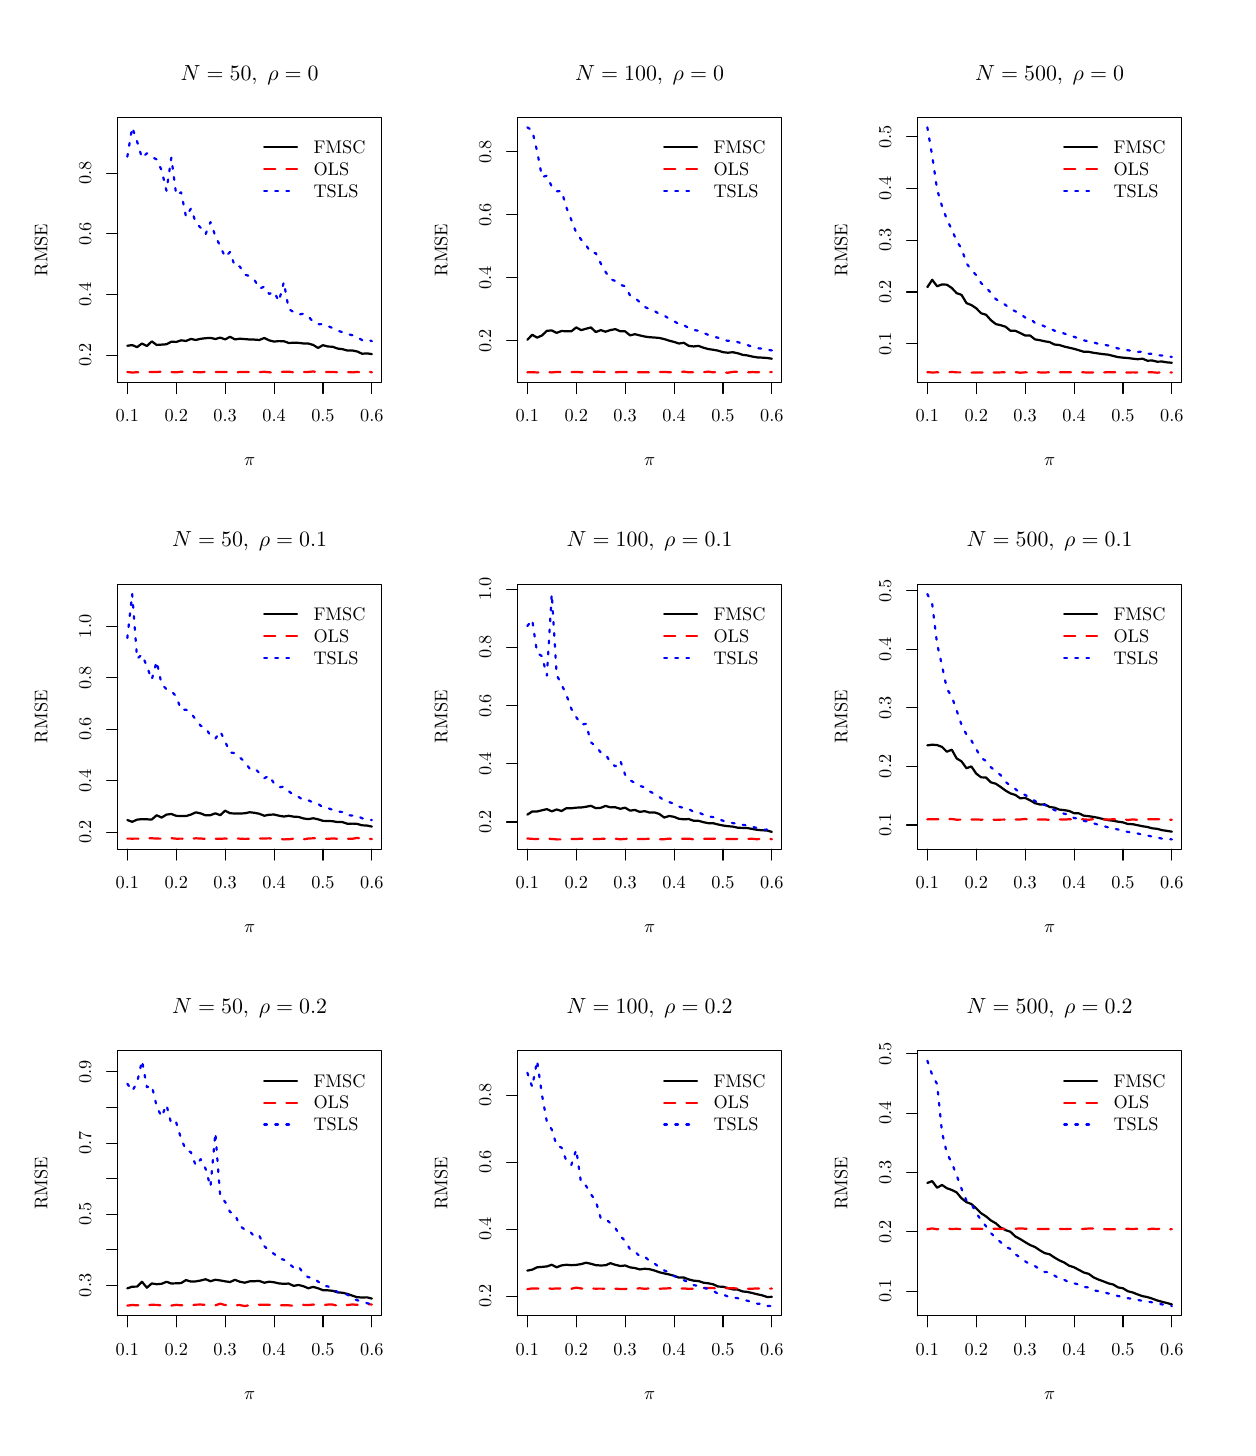
\begin{tikzpicture}[x=1pt,y=1pt]
\definecolor[named]{fillColor}{rgb}{1.00,1.00,1.00}
\path[use as bounding box,fill=fillColor,fill opacity=0.00] (0,0) rectangle (433.62,505.89);
\begin{scope}
\path[clip] ( 32.47,377.65) rectangle (127.91,473.42);
\definecolor[named]{drawColor}{rgb}{0.00,0.00,0.00}

\path[draw=drawColor,line width= 0.8pt,line join=round,line cap=round] ( 36.01,390.94) --
	( 37.77,391.19) --
	( 39.54,390.45) --
	( 41.31,391.76) --
	( 43.08,390.85) --
	( 44.84,392.53) --
	( 46.61,391.24) --
	( 48.38,391.36) --
	( 50.15,391.48) --
	( 51.91,392.41) --
	( 53.68,392.33) --
	( 55.45,392.91) --
	( 57.21,392.68) --
	( 58.98,393.41) --
	( 60.75,393.04) --
	( 62.52,393.46) --
	( 64.28,393.67) --
	( 66.05,393.80) --
	( 67.82,393.38) --
	( 69.59,393.90) --
	( 71.35,393.23) --
	( 73.12,394.20) --
	( 74.89,393.24) --
	( 76.66,393.49) --
	( 78.42,393.36) --
	( 80.19,393.21) --
	( 81.96,393.17) --
	( 83.72,393.03) --
	( 85.49,393.75) --
	( 87.26,392.90) --
	( 89.03,392.46) --
	( 90.79,392.62) --
	( 92.56,392.59) --
	( 94.33,391.96) --
	( 96.10,392.03) --
	( 97.86,391.99) --
	( 99.63,391.78) --
	(101.40,391.74) --
	(103.17,391.24) --
	(104.93,390.16) --
	(106.70,391.15) --
	(108.47,390.67) --
	(110.23,390.58) --
	(112.00,389.93) --
	(113.77,389.71) --
	(115.54,389.21) --
	(117.30,389.24) --
	(119.07,388.88) --
	(120.84,388.06) --
	(122.61,388.19) --
	(124.37,387.93);
\end{scope}
\begin{scope}
\path[clip] (  0.00,  0.00) rectangle (433.62,505.89);
\definecolor[named]{drawColor}{rgb}{0.00,0.00,0.00}

\path[draw=drawColor,line width= 0.4pt,line join=round,line cap=round] ( 36.01,377.65) -- (124.37,377.65);

\path[draw=drawColor,line width= 0.4pt,line join=round,line cap=round] ( 36.01,377.65) -- ( 36.01,373.69);

\path[draw=drawColor,line width= 0.4pt,line join=round,line cap=round] ( 53.68,377.65) -- ( 53.68,373.69);

\path[draw=drawColor,line width= 0.4pt,line join=round,line cap=round] ( 71.35,377.65) -- ( 71.35,373.69);

\path[draw=drawColor,line width= 0.4pt,line join=round,line cap=round] ( 89.03,377.65) -- ( 89.03,373.69);

\path[draw=drawColor,line width= 0.4pt,line join=round,line cap=round] (106.70,377.65) -- (106.70,373.69);

\path[draw=drawColor,line width= 0.4pt,line join=round,line cap=round] (124.37,377.65) -- (124.37,373.69);

\node[text=drawColor,anchor=base,inner sep=0pt, outer sep=0pt, scale=  0.66] at ( 36.01,363.40) {0.1};

\node[text=drawColor,anchor=base,inner sep=0pt, outer sep=0pt, scale=  0.66] at ( 53.68,363.40) {0.2};

\node[text=drawColor,anchor=base,inner sep=0pt, outer sep=0pt, scale=  0.66] at ( 71.35,363.40) {0.3};

\node[text=drawColor,anchor=base,inner sep=0pt, outer sep=0pt, scale=  0.66] at ( 89.03,363.40) {0.4};

\node[text=drawColor,anchor=base,inner sep=0pt, outer sep=0pt, scale=  0.66] at (106.70,363.40) {0.5};

\node[text=drawColor,anchor=base,inner sep=0pt, outer sep=0pt, scale=  0.66] at (124.37,363.40) {0.6};

\path[draw=drawColor,line width= 0.4pt,line join=round,line cap=round] ( 32.47,387.54) -- ( 32.47,453.30);

\path[draw=drawColor,line width= 0.4pt,line join=round,line cap=round] ( 32.47,387.54) -- ( 28.51,387.54);

\path[draw=drawColor,line width= 0.4pt,line join=round,line cap=round] ( 32.47,409.46) -- ( 28.51,409.46);

\path[draw=drawColor,line width= 0.4pt,line join=round,line cap=round] ( 32.47,431.38) -- ( 28.51,431.38);

\path[draw=drawColor,line width= 0.4pt,line join=round,line cap=round] ( 32.47,453.30) -- ( 28.51,453.30);

\node[text=drawColor,rotate= 90.00,anchor=base,inner sep=0pt, outer sep=0pt, scale=  0.66] at ( 22.97,387.54) {0.2};

\node[text=drawColor,rotate= 90.00,anchor=base,inner sep=0pt, outer sep=0pt, scale=  0.66] at ( 22.97,409.46) {0.4};

\node[text=drawColor,rotate= 90.00,anchor=base,inner sep=0pt, outer sep=0pt, scale=  0.66] at ( 22.97,431.38) {0.6};

\node[text=drawColor,rotate= 90.00,anchor=base,inner sep=0pt, outer sep=0pt, scale=  0.66] at ( 22.97,453.30) {0.8};

\path[draw=drawColor,line width= 0.4pt,line join=round,line cap=round] ( 32.47,377.65) --
	(127.91,377.65) --
	(127.91,473.42) --
	( 32.47,473.42) --
	( 32.47,377.65);
\end{scope}
\begin{scope}
\path[clip] (  0.00,337.26) rectangle (144.54,505.89);
\definecolor[named]{drawColor}{rgb}{0.00,0.00,0.00}

\node[text=drawColor,anchor=base,inner sep=0pt, outer sep=0pt, scale=  0.79] at ( 80.19,486.92) {\bfseries $N=50, \;\rho=0$};

\node[text=drawColor,anchor=base,inner sep=0pt, outer sep=0pt, scale=  0.66] at ( 80.19,347.56) {$\pi$};

\node[text=drawColor,rotate= 90.00,anchor=base,inner sep=0pt, outer sep=0pt, scale=  0.66] at (  7.13,425.53) {RMSE};
\end{scope}
\begin{scope}
\path[clip] ( 32.47,377.65) rectangle (127.91,473.42);
\definecolor[named]{drawColor}{rgb}{1.00,0.00,0.00}

\path[draw=drawColor,line width= 0.8pt,dash pattern=on 4pt off 4pt ,line join=round,line cap=round] ( 36.01,381.46) --
	( 37.77,381.27) --
	( 39.54,381.38) --
	( 41.31,381.37) --
	( 43.08,381.49) --
	( 44.84,381.46) --
	( 46.61,381.47) --
	( 48.38,381.58) --
	( 50.15,381.41) --
	( 51.91,381.43) --
	( 53.68,381.34) --
	( 55.45,381.55) --
	( 57.21,381.46) --
	( 58.98,381.48) --
	( 60.75,381.42) --
	( 62.52,381.36) --
	( 64.28,381.55) --
	( 66.05,381.46) --
	( 67.82,381.43) --
	( 69.59,381.46) --
	( 71.35,381.47) --
	( 73.12,381.41) --
	( 74.89,381.20) --
	( 76.66,381.47) --
	( 78.42,381.49) --
	( 80.19,381.43) --
	( 81.96,381.23) --
	( 83.72,381.41) --
	( 85.49,381.55) --
	( 87.26,381.36) --
	( 89.03,381.22) --
	( 90.79,381.34) --
	( 92.56,381.59) --
	( 94.33,381.59) --
	( 96.10,381.35) --
	( 97.86,381.39) --
	( 99.63,381.45) --
	(101.40,381.49) --
	(103.17,381.66) --
	(104.93,381.31) --
	(106.70,381.52) --
	(108.47,381.45) --
	(110.23,381.44) --
	(112.00,381.39) --
	(113.77,381.43) --
	(115.54,381.45) --
	(117.30,381.32) --
	(119.07,381.48) --
	(120.84,381.28) --
	(122.61,381.67) --
	(124.37,381.36);
\definecolor[named]{drawColor}{rgb}{0.00,0.00,1.00}

\path[draw=drawColor,line width= 0.8pt,dash pattern=on 1pt off 3pt ,line join=round,line cap=round] ( 36.01,459.27) --
	( 37.77,469.87) --
	( 39.54,464.75) --
	( 41.31,458.79) --
	( 43.08,460.51) --
	( 44.84,459.16) --
	( 46.61,458.27) --
	( 48.38,454.40) --
	( 50.15,446.99) --
	( 51.91,458.89) --
	( 53.68,445.44) --
	( 55.45,446.39) --
	( 57.21,437.53) --
	( 58.98,440.52) --
	( 60.75,435.49) --
	( 62.52,433.55) --
	( 64.28,431.23) --
	( 66.05,435.62) --
	( 67.82,430.58) --
	( 69.59,426.86) --
	( 71.35,422.97) --
	( 73.12,424.82) --
	( 74.89,419.58) --
	( 76.66,419.59) --
	( 78.42,416.67) --
	( 80.19,416.13) --
	( 81.96,414.74) --
	( 83.72,411.58) --
	( 85.49,412.29) --
	( 87.26,409.67) --
	( 89.03,410.48) --
	( 90.79,406.99) --
	( 92.56,413.94) --
	( 94.33,404.18) --
	( 96.10,403.14) --
	( 97.86,402.21) --
	( 99.63,402.52) --
	(101.40,401.55) --
	(103.17,399.59) --
	(104.93,398.75) --
	(106.70,398.76) --
	(108.47,398.06) --
	(110.23,397.33) --
	(112.00,396.38) --
	(113.77,395.86) --
	(115.54,395.23) --
	(117.30,394.74) --
	(119.07,394.09) --
	(120.84,392.99) --
	(122.61,393.25) --
	(124.37,392.61);
\definecolor[named]{drawColor}{rgb}{0.00,0.00,0.00}

\path[draw=drawColor,line width= 0.8pt,line join=round,line cap=round] ( 85.47,462.63) -- ( 97.35,462.63);
\definecolor[named]{drawColor}{rgb}{1.00,0.00,0.00}

\path[draw=drawColor,line width= 0.8pt,dash pattern=on 4pt off 4pt ,line join=round,line cap=round] ( 85.47,454.71) -- ( 97.35,454.71);
\definecolor[named]{drawColor}{rgb}{0.00,0.00,1.00}

\path[draw=drawColor,line width= 0.8pt,dash pattern=on 1pt off 3pt ,line join=round,line cap=round] ( 85.47,446.79) -- ( 97.35,446.79);
\definecolor[named]{drawColor}{rgb}{0.00,0.00,0.00}

\node[text=drawColor,anchor=base west,inner sep=0pt, outer sep=0pt, scale=  0.66] at (103.29,460.35) {FMSC};

\node[text=drawColor,anchor=base west,inner sep=0pt, outer sep=0pt, scale=  0.66] at (103.29,452.43) {OLS};

\node[text=drawColor,anchor=base west,inner sep=0pt, outer sep=0pt, scale=  0.66] at (103.29,444.51) {TSLS};
\end{scope}
\begin{scope}
\path[clip] (177.01,377.65) rectangle (272.45,473.42);
\definecolor[named]{drawColor}{rgb}{0.00,0.00,0.00}

\path[draw=drawColor,line width= 0.8pt,line join=round,line cap=round] (180.55,393.08) --
	(182.31,394.92) --
	(184.08,393.88) --
	(185.85,394.67) --
	(187.62,396.35) --
	(189.38,396.48) --
	(191.15,395.61) --
	(192.92,396.28) --
	(194.69,396.17) --
	(196.45,396.15) --
	(198.22,397.58) --
	(199.99,396.59) --
	(201.75,397.08) --
	(203.52,397.56) --
	(205.29,395.90) --
	(207.06,396.59) --
	(208.82,396.02) --
	(210.59,396.62) --
	(212.36,396.94) --
	(214.13,396.19) --
	(215.89,396.15) --
	(217.66,394.70) --
	(219.43,395.12) --
	(221.20,394.68) --
	(222.96,394.28) --
	(224.73,394.03) --
	(226.50,393.92) --
	(228.26,393.76) --
	(230.03,393.35) --
	(231.80,392.79) --
	(233.57,392.33) --
	(235.33,391.75) --
	(237.10,392.02) --
	(238.87,390.91) --
	(240.64,390.69) --
	(242.40,390.90) --
	(244.17,390.25) --
	(245.94,389.75) --
	(247.71,389.50) --
	(249.47,389.18) --
	(251.24,388.63) --
	(253.01,388.43) --
	(254.77,388.61) --
	(256.54,388.25) --
	(258.31,387.67) --
	(260.08,387.45) --
	(261.84,387.04) --
	(263.61,386.74) --
	(265.38,386.65) --
	(267.15,386.53) --
	(268.91,386.26);
\end{scope}
\begin{scope}
\path[clip] (  0.00,  0.00) rectangle (433.62,505.89);
\definecolor[named]{drawColor}{rgb}{0.00,0.00,0.00}

\path[draw=drawColor,line width= 0.4pt,line join=round,line cap=round] (180.55,377.65) -- (268.91,377.65);

\path[draw=drawColor,line width= 0.4pt,line join=round,line cap=round] (180.55,377.65) -- (180.55,373.69);

\path[draw=drawColor,line width= 0.4pt,line join=round,line cap=round] (198.22,377.65) -- (198.22,373.69);

\path[draw=drawColor,line width= 0.4pt,line join=round,line cap=round] (215.89,377.65) -- (215.89,373.69);

\path[draw=drawColor,line width= 0.4pt,line join=round,line cap=round] (233.57,377.65) -- (233.57,373.69);

\path[draw=drawColor,line width= 0.4pt,line join=round,line cap=round] (251.24,377.65) -- (251.24,373.69);

\path[draw=drawColor,line width= 0.4pt,line join=round,line cap=round] (268.91,377.65) -- (268.91,373.69);

\node[text=drawColor,anchor=base,inner sep=0pt, outer sep=0pt, scale=  0.66] at (180.55,363.40) {0.1};

\node[text=drawColor,anchor=base,inner sep=0pt, outer sep=0pt, scale=  0.66] at (198.22,363.40) {0.2};

\node[text=drawColor,anchor=base,inner sep=0pt, outer sep=0pt, scale=  0.66] at (215.89,363.40) {0.3};

\node[text=drawColor,anchor=base,inner sep=0pt, outer sep=0pt, scale=  0.66] at (233.57,363.40) {0.4};

\node[text=drawColor,anchor=base,inner sep=0pt, outer sep=0pt, scale=  0.66] at (251.24,363.40) {0.5};

\node[text=drawColor,anchor=base,inner sep=0pt, outer sep=0pt, scale=  0.66] at (268.91,363.40) {0.6};

\path[draw=drawColor,line width= 0.4pt,line join=round,line cap=round] (177.01,392.72) -- (177.01,461.10);

\path[draw=drawColor,line width= 0.4pt,line join=round,line cap=round] (177.01,392.72) -- (173.05,392.72);

\path[draw=drawColor,line width= 0.4pt,line join=round,line cap=round] (177.01,415.51) -- (173.05,415.51);

\path[draw=drawColor,line width= 0.4pt,line join=round,line cap=round] (177.01,438.31) -- (173.05,438.31);

\path[draw=drawColor,line width= 0.4pt,line join=round,line cap=round] (177.01,461.10) -- (173.05,461.10);

\node[text=drawColor,rotate= 90.00,anchor=base,inner sep=0pt, outer sep=0pt, scale=  0.66] at (167.51,392.72) {0.2};

\node[text=drawColor,rotate= 90.00,anchor=base,inner sep=0pt, outer sep=0pt, scale=  0.66] at (167.51,415.51) {0.4};

\node[text=drawColor,rotate= 90.00,anchor=base,inner sep=0pt, outer sep=0pt, scale=  0.66] at (167.51,438.31) {0.6};

\node[text=drawColor,rotate= 90.00,anchor=base,inner sep=0pt, outer sep=0pt, scale=  0.66] at (167.51,461.10) {0.8};

\path[draw=drawColor,line width= 0.4pt,line join=round,line cap=round] (177.01,377.65) --
	(272.45,377.65) --
	(272.45,473.42) --
	(177.01,473.42) --
	(177.01,377.65);
\end{scope}
\begin{scope}
\path[clip] (144.54,337.26) rectangle (289.08,505.89);
\definecolor[named]{drawColor}{rgb}{0.00,0.00,0.00}

\node[text=drawColor,anchor=base,inner sep=0pt, outer sep=0pt, scale=  0.79] at (224.73,486.92) {\bfseries $N=100, \;\rho=0$};

\node[text=drawColor,anchor=base,inner sep=0pt, outer sep=0pt, scale=  0.66] at (224.73,347.56) {$\pi$};

\node[text=drawColor,rotate= 90.00,anchor=base,inner sep=0pt, outer sep=0pt, scale=  0.66] at (151.67,425.53) {RMSE};
\end{scope}
\begin{scope}
\path[clip] (177.01,377.65) rectangle (272.45,473.42);
\definecolor[named]{drawColor}{rgb}{1.00,0.00,0.00}

\path[draw=drawColor,line width= 0.8pt,dash pattern=on 4pt off 4pt ,line join=round,line cap=round] (180.55,381.35) --
	(182.31,381.37) --
	(184.08,381.31) --
	(185.85,381.36) --
	(187.62,381.46) --
	(189.38,381.31) --
	(191.15,381.48) --
	(192.92,381.41) --
	(194.69,381.34) --
	(196.45,381.41) --
	(198.22,381.49) --
	(199.99,381.38) --
	(201.75,381.37) --
	(203.52,381.38) --
	(205.29,381.57) --
	(207.06,381.50) --
	(208.82,381.44) --
	(210.59,381.50) --
	(212.36,381.34) --
	(214.13,381.47) --
	(215.89,381.44) --
	(217.66,381.39) --
	(219.43,381.40) --
	(221.20,381.37) --
	(222.96,381.34) --
	(224.73,381.35) --
	(226.50,381.43) --
	(228.26,381.43) --
	(230.03,381.48) --
	(231.80,381.37) --
	(233.57,381.41) --
	(235.33,381.33) --
	(237.10,381.61) --
	(238.87,381.34) --
	(240.64,381.36) --
	(242.40,381.48) --
	(244.17,381.39) --
	(245.94,381.61) --
	(247.71,381.33) --
	(249.47,381.55) --
	(251.24,381.36) --
	(253.01,381.20) --
	(254.77,381.51) --
	(256.54,381.54) --
	(258.31,381.29) --
	(260.08,381.32) --
	(261.84,381.44) --
	(263.61,381.37) --
	(265.38,381.41) --
	(267.15,381.32) --
	(268.91,381.46);
\definecolor[named]{drawColor}{rgb}{0.00,0.00,1.00}

\path[draw=drawColor,line width= 0.8pt,dash pattern=on 1pt off 3pt ,line join=round,line cap=round] (180.55,469.87) --
	(182.31,468.74) --
	(184.08,461.22) --
	(185.85,451.91) --
	(187.62,452.40) --
	(189.38,448.43) --
	(191.15,446.74) --
	(192.92,446.90) --
	(194.69,440.84) --
	(196.45,436.40) --
	(198.22,431.80) --
	(199.99,429.31) --
	(201.75,427.32) --
	(203.52,424.54) --
	(205.29,424.41) --
	(207.06,420.72) --
	(208.82,417.61) --
	(210.59,414.97) --
	(212.36,414.38) --
	(214.13,413.00) --
	(215.89,412.40) --
	(217.66,409.16) --
	(219.43,408.28) --
	(221.20,406.64) --
	(222.96,404.98) --
	(224.73,404.17) --
	(226.50,403.51) --
	(228.26,402.42) --
	(230.03,401.85) --
	(231.80,400.71) --
	(233.57,399.85) --
	(235.33,398.72) --
	(237.10,398.43) --
	(238.87,397.30) --
	(240.64,396.66) --
	(242.40,396.35) --
	(244.17,395.60) --
	(245.94,394.87) --
	(247.71,394.26) --
	(249.47,393.84) --
	(251.24,393.09) --
	(253.01,392.73) --
	(254.77,392.83) --
	(256.54,392.28) --
	(258.31,391.72) --
	(260.08,391.20) --
	(261.84,390.60) --
	(263.61,390.07) --
	(265.38,389.90) --
	(267.15,389.53) --
	(268.91,389.25);
\definecolor[named]{drawColor}{rgb}{0.00,0.00,0.00}

\path[draw=drawColor,line width= 0.8pt,line join=round,line cap=round] (230.01,462.63) -- (241.89,462.63);
\definecolor[named]{drawColor}{rgb}{1.00,0.00,0.00}

\path[draw=drawColor,line width= 0.8pt,dash pattern=on 4pt off 4pt ,line join=round,line cap=round] (230.01,454.71) -- (241.89,454.71);
\definecolor[named]{drawColor}{rgb}{0.00,0.00,1.00}

\path[draw=drawColor,line width= 0.8pt,dash pattern=on 1pt off 3pt ,line join=round,line cap=round] (230.01,446.79) -- (241.89,446.79);
\definecolor[named]{drawColor}{rgb}{0.00,0.00,0.00}

\node[text=drawColor,anchor=base west,inner sep=0pt, outer sep=0pt, scale=  0.66] at (247.83,460.35) {FMSC};

\node[text=drawColor,anchor=base west,inner sep=0pt, outer sep=0pt, scale=  0.66] at (247.83,452.43) {OLS};

\node[text=drawColor,anchor=base west,inner sep=0pt, outer sep=0pt, scale=  0.66] at (247.83,444.51) {TSLS};
\end{scope}
\begin{scope}
\path[clip] (321.55,377.65) rectangle (416.99,473.42);
\definecolor[named]{drawColor}{rgb}{0.00,0.00,0.00}

\path[draw=drawColor,line width= 0.8pt,line join=round,line cap=round] (325.09,412.12) --
	(326.85,414.78) --
	(328.62,412.44) --
	(330.39,413.10) --
	(332.16,413.01) --
	(333.92,411.81) --
	(335.69,409.95) --
	(337.46,409.33) --
	(339.23,406.35) --
	(340.99,405.66) --
	(342.76,404.49) --
	(344.53,402.67) --
	(346.29,402.16) --
	(348.06,400.19) --
	(349.83,398.78) --
	(351.60,398.37) --
	(353.36,397.82) --
	(355.13,396.36) --
	(356.90,396.34) --
	(358.67,395.54) --
	(360.43,394.64) --
	(362.20,394.67) --
	(363.97,393.25) --
	(365.74,392.95) --
	(367.50,392.55) --
	(369.27,392.28) --
	(371.04,391.39) --
	(372.80,391.22) --
	(374.57,390.65) --
	(376.34,390.24) --
	(378.11,389.83) --
	(379.87,389.32) --
	(381.64,388.76) --
	(383.41,388.75) --
	(385.18,388.39) --
	(386.94,388.14) --
	(388.71,387.90) --
	(390.48,387.72) --
	(392.25,387.27) --
	(394.01,386.84) --
	(395.78,386.65) --
	(397.55,386.51) --
	(399.31,386.28) --
	(401.08,386.08) --
	(402.85,386.27) --
	(404.62,385.55) --
	(406.38,385.61) --
	(408.15,385.19) --
	(409.92,385.24) --
	(411.69,384.95) --
	(413.45,384.80);
\end{scope}
\begin{scope}
\path[clip] (  0.00,  0.00) rectangle (433.62,505.89);
\definecolor[named]{drawColor}{rgb}{0.00,0.00,0.00}

\path[draw=drawColor,line width= 0.4pt,line join=round,line cap=round] (325.09,377.65) -- (413.45,377.65);

\path[draw=drawColor,line width= 0.4pt,line join=round,line cap=round] (325.09,377.65) -- (325.09,373.69);

\path[draw=drawColor,line width= 0.4pt,line join=round,line cap=round] (342.76,377.65) -- (342.76,373.69);

\path[draw=drawColor,line width= 0.4pt,line join=round,line cap=round] (360.43,377.65) -- (360.43,373.69);

\path[draw=drawColor,line width= 0.4pt,line join=round,line cap=round] (378.11,377.65) -- (378.11,373.69);

\path[draw=drawColor,line width= 0.4pt,line join=round,line cap=round] (395.78,377.65) -- (395.78,373.69);

\path[draw=drawColor,line width= 0.4pt,line join=round,line cap=round] (413.45,377.65) -- (413.45,373.69);

\node[text=drawColor,anchor=base,inner sep=0pt, outer sep=0pt, scale=  0.66] at (325.09,363.40) {0.1};

\node[text=drawColor,anchor=base,inner sep=0pt, outer sep=0pt, scale=  0.66] at (342.76,363.40) {0.2};

\node[text=drawColor,anchor=base,inner sep=0pt, outer sep=0pt, scale=  0.66] at (360.43,363.40) {0.3};

\node[text=drawColor,anchor=base,inner sep=0pt, outer sep=0pt, scale=  0.66] at (378.11,363.40) {0.4};

\node[text=drawColor,anchor=base,inner sep=0pt, outer sep=0pt, scale=  0.66] at (395.78,363.40) {0.5};

\node[text=drawColor,anchor=base,inner sep=0pt, outer sep=0pt, scale=  0.66] at (413.45,363.40) {0.6};

\path[draw=drawColor,line width= 0.4pt,line join=round,line cap=round] (321.55,391.66) -- (321.55,466.55);

\path[draw=drawColor,line width= 0.4pt,line join=round,line cap=round] (321.55,391.66) -- (317.59,391.66);

\path[draw=drawColor,line width= 0.4pt,line join=round,line cap=round] (321.55,410.38) -- (317.59,410.38);

\path[draw=drawColor,line width= 0.4pt,line join=round,line cap=round] (321.55,429.11) -- (317.59,429.11);

\path[draw=drawColor,line width= 0.4pt,line join=round,line cap=round] (321.55,447.83) -- (317.59,447.83);

\path[draw=drawColor,line width= 0.4pt,line join=round,line cap=round] (321.55,466.55) -- (317.59,466.55);

\node[text=drawColor,rotate= 90.00,anchor=base,inner sep=0pt, outer sep=0pt, scale=  0.66] at (312.05,391.66) {0.1};

\node[text=drawColor,rotate= 90.00,anchor=base,inner sep=0pt, outer sep=0pt, scale=  0.66] at (312.05,410.38) {0.2};

\node[text=drawColor,rotate= 90.00,anchor=base,inner sep=0pt, outer sep=0pt, scale=  0.66] at (312.05,429.11) {0.3};

\node[text=drawColor,rotate= 90.00,anchor=base,inner sep=0pt, outer sep=0pt, scale=  0.66] at (312.05,447.83) {0.4};

\node[text=drawColor,rotate= 90.00,anchor=base,inner sep=0pt, outer sep=0pt, scale=  0.66] at (312.05,466.55) {0.5};

\path[draw=drawColor,line width= 0.4pt,line join=round,line cap=round] (321.55,377.65) --
	(416.99,377.65) --
	(416.99,473.42) --
	(321.55,473.42) --
	(321.55,377.65);
\end{scope}
\begin{scope}
\path[clip] (289.08,337.26) rectangle (433.62,505.89);
\definecolor[named]{drawColor}{rgb}{0.00,0.00,0.00}

\node[text=drawColor,anchor=base,inner sep=0pt, outer sep=0pt, scale=  0.79] at (369.27,486.92) {\bfseries $N=500, \;\rho=0$};

\node[text=drawColor,anchor=base,inner sep=0pt, outer sep=0pt, scale=  0.66] at (369.27,347.56) {$\pi$};

\node[text=drawColor,rotate= 90.00,anchor=base,inner sep=0pt, outer sep=0pt, scale=  0.66] at (296.21,425.53) {RMSE};
\end{scope}
\begin{scope}
\path[clip] (321.55,377.65) rectangle (416.99,473.42);
\definecolor[named]{drawColor}{rgb}{1.00,0.00,0.00}

\path[draw=drawColor,line width= 0.8pt,dash pattern=on 4pt off 4pt ,line join=round,line cap=round] (325.09,381.40) --
	(326.85,381.29) --
	(328.62,381.35) --
	(330.39,381.25) --
	(332.16,381.31) --
	(333.92,381.49) --
	(335.69,381.33) --
	(337.46,381.33) --
	(339.23,381.39) --
	(340.99,381.23) --
	(342.76,381.29) --
	(344.53,381.28) --
	(346.29,381.36) --
	(348.06,381.27) --
	(349.83,381.27) --
	(351.60,381.33) --
	(353.36,381.35) --
	(355.13,381.27) --
	(356.90,381.41) --
	(358.67,381.21) --
	(360.43,381.34) --
	(362.20,381.29) --
	(363.97,381.40) --
	(365.74,381.32) --
	(367.50,381.28) --
	(369.27,381.38) --
	(371.04,381.28) --
	(372.80,381.38) --
	(374.57,381.35) --
	(376.34,381.36) --
	(378.11,381.36) --
	(379.87,381.45) --
	(381.64,381.34) --
	(383.41,381.27) --
	(385.18,381.32) --
	(386.94,381.20) --
	(388.71,381.29) --
	(390.48,381.42) --
	(392.25,381.34) --
	(394.01,381.40) --
	(395.78,381.39) --
	(397.55,381.27) --
	(399.31,381.33) --
	(401.08,381.29) --
	(402.85,381.39) --
	(404.62,381.40) --
	(406.38,381.36) --
	(408.15,381.21) --
	(409.92,381.36) --
	(411.69,381.30) --
	(413.45,381.31);
\definecolor[named]{drawColor}{rgb}{0.00,0.00,1.00}

\path[draw=drawColor,line width= 0.8pt,dash pattern=on 1pt off 3pt ,line join=round,line cap=round] (325.09,469.87) --
	(326.85,459.55) --
	(328.62,447.41) --
	(330.39,441.39) --
	(332.16,436.57) --
	(333.92,432.96) --
	(335.69,428.78) --
	(337.46,426.04) --
	(339.23,420.73) --
	(340.99,418.39) --
	(342.76,416.42) --
	(344.53,413.59) --
	(346.29,412.06) --
	(348.06,410.01) --
	(349.83,407.80) --
	(351.60,406.83) --
	(353.36,405.67) --
	(355.13,404.28) --
	(356.90,403.39) --
	(358.67,402.48) --
	(360.43,401.15) --
	(362.20,400.84) --
	(363.97,399.20) --
	(365.74,398.72) --
	(367.50,397.92) --
	(369.27,397.36) --
	(371.04,396.38) --
	(372.80,395.93) --
	(374.57,395.37) --
	(376.34,394.62) --
	(378.11,394.18) --
	(379.87,393.53) --
	(381.64,392.91) --
	(383.41,392.51) --
	(385.18,392.17) --
	(386.94,391.61) --
	(388.71,391.38) --
	(390.48,391.01) --
	(392.25,390.41) --
	(394.01,389.97) --
	(395.78,389.66) --
	(397.55,389.33) --
	(399.31,389.03) --
	(401.08,388.70) --
	(402.85,388.85) --
	(404.62,388.10) --
	(406.38,388.01) --
	(408.15,387.54) --
	(409.92,387.43) --
	(411.69,387.12) --
	(413.45,386.91);
\definecolor[named]{drawColor}{rgb}{0.00,0.00,0.00}

\path[draw=drawColor,line width= 0.8pt,line join=round,line cap=round] (374.55,462.63) -- (386.43,462.63);
\definecolor[named]{drawColor}{rgb}{1.00,0.00,0.00}

\path[draw=drawColor,line width= 0.8pt,dash pattern=on 4pt off 4pt ,line join=round,line cap=round] (374.55,454.71) -- (386.43,454.71);
\definecolor[named]{drawColor}{rgb}{0.00,0.00,1.00}

\path[draw=drawColor,line width= 0.8pt,dash pattern=on 1pt off 3pt ,line join=round,line cap=round] (374.55,446.79) -- (386.43,446.79);
\definecolor[named]{drawColor}{rgb}{0.00,0.00,0.00}

\node[text=drawColor,anchor=base west,inner sep=0pt, outer sep=0pt, scale=  0.66] at (392.37,460.35) {FMSC};

\node[text=drawColor,anchor=base west,inner sep=0pt, outer sep=0pt, scale=  0.66] at (392.37,452.43) {OLS};

\node[text=drawColor,anchor=base west,inner sep=0pt, outer sep=0pt, scale=  0.66] at (392.37,444.51) {TSLS};
\end{scope}
\begin{scope}
\path[clip] ( 32.47,209.02) rectangle (127.91,304.79);
\definecolor[named]{drawColor}{rgb}{0.00,0.00,0.00}

\path[draw=drawColor,line width= 0.8pt,line join=round,line cap=round] ( 36.01,219.56) --
	( 37.77,218.93) --
	( 39.54,219.71) --
	( 41.31,219.90) --
	( 43.08,219.83) --
	( 44.84,219.74) --
	( 46.61,221.31) --
	( 48.38,220.44) --
	( 50.15,221.53) --
	( 51.91,221.75) --
	( 53.68,221.09) --
	( 55.45,221.00) --
	( 57.21,221.00) --
	( 58.98,221.54) --
	( 60.75,222.35) --
	( 62.52,221.96) --
	( 64.28,221.25) --
	( 66.05,221.33) --
	( 67.82,221.99) --
	( 69.59,221.31) --
	( 71.35,222.96) --
	( 73.12,222.02) --
	( 74.89,221.93) --
	( 76.66,221.92) --
	( 78.42,222.00) --
	( 80.19,222.38) --
	( 81.96,222.19) --
	( 83.72,221.82) --
	( 85.49,221.12) --
	( 87.26,221.48) --
	( 89.03,221.56) --
	( 90.79,221.13) --
	( 92.56,220.83) --
	( 94.33,221.10) --
	( 96.10,220.79) --
	( 97.86,220.69) --
	( 99.63,220.15) --
	(101.40,219.89) --
	(103.17,220.21) --
	(104.93,219.84) --
	(106.70,219.26) --
	(108.47,219.25) --
	(110.23,219.14) --
	(112.00,218.82) --
	(113.77,218.82) --
	(115.54,218.22) --
	(117.30,218.27) --
	(119.07,218.17) --
	(120.84,217.66) --
	(122.61,217.58) --
	(124.37,217.20);
\end{scope}
\begin{scope}
\path[clip] (  0.00,  0.00) rectangle (433.62,505.89);
\definecolor[named]{drawColor}{rgb}{0.00,0.00,0.00}

\path[draw=drawColor,line width= 0.4pt,line join=round,line cap=round] ( 36.01,209.02) -- (124.37,209.02);

\path[draw=drawColor,line width= 0.4pt,line join=round,line cap=round] ( 36.01,209.02) -- ( 36.01,205.06);

\path[draw=drawColor,line width= 0.4pt,line join=round,line cap=round] ( 53.68,209.02) -- ( 53.68,205.06);

\path[draw=drawColor,line width= 0.4pt,line join=round,line cap=round] ( 71.35,209.02) -- ( 71.35,205.06);

\path[draw=drawColor,line width= 0.4pt,line join=round,line cap=round] ( 89.03,209.02) -- ( 89.03,205.06);

\path[draw=drawColor,line width= 0.4pt,line join=round,line cap=round] (106.70,209.02) -- (106.70,205.06);

\path[draw=drawColor,line width= 0.4pt,line join=round,line cap=round] (124.37,209.02) -- (124.37,205.06);

\node[text=drawColor,anchor=base,inner sep=0pt, outer sep=0pt, scale=  0.66] at ( 36.01,194.77) {0.1};

\node[text=drawColor,anchor=base,inner sep=0pt, outer sep=0pt, scale=  0.66] at ( 53.68,194.77) {0.2};

\node[text=drawColor,anchor=base,inner sep=0pt, outer sep=0pt, scale=  0.66] at ( 71.35,194.77) {0.3};

\node[text=drawColor,anchor=base,inner sep=0pt, outer sep=0pt, scale=  0.66] at ( 89.03,194.77) {0.4};

\node[text=drawColor,anchor=base,inner sep=0pt, outer sep=0pt, scale=  0.66] at (106.70,194.77) {0.5};

\node[text=drawColor,anchor=base,inner sep=0pt, outer sep=0pt, scale=  0.66] at (124.37,194.77) {0.6};

\path[draw=drawColor,line width= 0.4pt,line join=round,line cap=round] ( 32.47,215.20) -- ( 32.47,289.53);

\path[draw=drawColor,line width= 0.4pt,line join=round,line cap=round] ( 32.47,215.20) -- ( 28.51,215.20);

\path[draw=drawColor,line width= 0.4pt,line join=round,line cap=round] ( 32.47,233.78) -- ( 28.51,233.78);

\path[draw=drawColor,line width= 0.4pt,line join=round,line cap=round] ( 32.47,252.36) -- ( 28.51,252.36);

\path[draw=drawColor,line width= 0.4pt,line join=round,line cap=round] ( 32.47,270.95) -- ( 28.51,270.95);

\path[draw=drawColor,line width= 0.4pt,line join=round,line cap=round] ( 32.47,289.53) -- ( 28.51,289.53);

\node[text=drawColor,rotate= 90.00,anchor=base,inner sep=0pt, outer sep=0pt, scale=  0.66] at ( 22.97,215.20) {0.2};

\node[text=drawColor,rotate= 90.00,anchor=base,inner sep=0pt, outer sep=0pt, scale=  0.66] at ( 22.97,233.78) {0.4};

\node[text=drawColor,rotate= 90.00,anchor=base,inner sep=0pt, outer sep=0pt, scale=  0.66] at ( 22.97,252.36) {0.6};

\node[text=drawColor,rotate= 90.00,anchor=base,inner sep=0pt, outer sep=0pt, scale=  0.66] at ( 22.97,270.95) {0.8};

\node[text=drawColor,rotate= 90.00,anchor=base,inner sep=0pt, outer sep=0pt, scale=  0.66] at ( 22.97,289.53) {1.0};

\path[draw=drawColor,line width= 0.4pt,line join=round,line cap=round] ( 32.47,209.02) --
	(127.91,209.02) --
	(127.91,304.79) --
	( 32.47,304.79) --
	( 32.47,209.02);
\end{scope}
\begin{scope}
\path[clip] (  0.00,168.63) rectangle (144.54,337.26);
\definecolor[named]{drawColor}{rgb}{0.00,0.00,0.00}

\node[text=drawColor,anchor=base,inner sep=0pt, outer sep=0pt, scale=  0.79] at ( 80.19,318.29) {\bfseries $N=50, \;\rho=0.1$};

\node[text=drawColor,anchor=base,inner sep=0pt, outer sep=0pt, scale=  0.66] at ( 80.19,178.93) {$\pi$};

\node[text=drawColor,rotate= 90.00,anchor=base,inner sep=0pt, outer sep=0pt, scale=  0.66] at (  7.13,256.90) {RMSE};
\end{scope}
\begin{scope}
\path[clip] ( 32.47,209.02) rectangle (127.91,304.79);
\definecolor[named]{drawColor}{rgb}{1.00,0.00,0.00}

\path[draw=drawColor,line width= 0.8pt,dash pattern=on 4pt off 4pt ,line join=round,line cap=round] ( 36.01,212.85) --
	( 37.77,212.84) --
	( 39.54,212.85) --
	( 41.31,212.81) --
	( 43.08,212.96) --
	( 44.84,212.97) --
	( 46.61,212.87) --
	( 48.38,212.84) --
	( 50.15,212.97) --
	( 51.91,213.01) --
	( 53.68,212.83) --
	( 55.45,212.85) --
	( 57.21,212.80) --
	( 58.98,212.81) --
	( 60.75,212.96) --
	( 62.52,212.90) --
	( 64.28,212.74) --
	( 66.05,212.83) --
	( 67.82,212.82) --
	( 69.59,212.78) --
	( 71.35,212.89) --
	( 73.12,212.73) --
	( 74.89,212.95) --
	( 76.66,212.84) --
	( 78.42,212.75) --
	( 80.19,212.79) --
	( 81.96,212.64) --
	( 83.72,212.88) --
	( 85.49,212.91) --
	( 87.26,212.95) --
	( 89.03,212.80) --
	( 90.79,212.84) --
	( 92.56,212.57) --
	( 94.33,212.63) --
	( 96.10,212.85) --
	( 97.86,212.91) --
	( 99.63,212.61) --
	(101.40,212.87) --
	(103.17,212.97) --
	(104.93,212.95) --
	(106.70,212.88) --
	(108.47,212.75) --
	(110.23,212.93) --
	(112.00,212.79) --
	(113.77,213.11) --
	(115.54,212.81) --
	(117.30,212.79) --
	(119.07,213.12) --
	(120.84,212.83) --
	(122.61,212.91) --
	(124.37,212.68);
\definecolor[named]{drawColor}{rgb}{0.00,0.00,1.00}

\path[draw=drawColor,line width= 0.8pt,dash pattern=on 1pt off 3pt ,line join=round,line cap=round] ( 36.01,285.33) --
	( 37.77,301.24) --
	( 39.54,277.88) --
	( 41.31,279.34) --
	( 43.08,275.10) --
	( 44.84,270.29) --
	( 46.61,276.88) --
	( 48.38,268.71) --
	( 50.15,266.84) --
	( 51.91,266.20) --
	( 53.68,264.22) --
	( 55.45,259.36) --
	( 57.21,259.47) --
	( 58.98,258.20) --
	( 60.75,255.86) --
	( 62.52,253.61) --
	( 64.28,252.89) --
	( 66.05,250.06) --
	( 67.82,248.98) --
	( 69.59,251.60) --
	( 71.35,247.94) --
	( 73.12,243.98) --
	( 74.89,243.75) --
	( 76.66,242.17) --
	( 78.42,240.62) --
	( 80.19,238.16) --
	( 81.96,238.37) --
	( 83.72,236.57) --
	( 85.49,234.64) --
	( 87.26,235.65) --
	( 89.03,232.76) --
	( 90.79,231.39) --
	( 92.56,231.63) --
	( 94.33,229.97) --
	( 96.10,228.61) --
	( 97.86,227.92) --
	( 99.63,226.79) --
	(101.40,226.72) --
	(103.17,225.89) --
	(104.93,225.41) --
	(106.70,224.16) --
	(108.47,223.89) --
	(110.23,223.23) --
	(112.00,222.58) --
	(113.77,222.49) --
	(115.54,221.34) --
	(117.30,221.19) --
	(119.07,221.10) --
	(120.84,220.21) --
	(122.61,219.75) --
	(124.37,219.58);
\definecolor[named]{drawColor}{rgb}{0.00,0.00,0.00}

\path[draw=drawColor,line width= 0.8pt,line join=round,line cap=round] ( 85.47,294.00) -- ( 97.35,294.00);
\definecolor[named]{drawColor}{rgb}{1.00,0.00,0.00}

\path[draw=drawColor,line width= 0.8pt,dash pattern=on 4pt off 4pt ,line join=round,line cap=round] ( 85.47,286.08) -- ( 97.35,286.08);
\definecolor[named]{drawColor}{rgb}{0.00,0.00,1.00}

\path[draw=drawColor,line width= 0.8pt,dash pattern=on 1pt off 3pt ,line join=round,line cap=round] ( 85.47,278.16) -- ( 97.35,278.16);
\definecolor[named]{drawColor}{rgb}{0.00,0.00,0.00}

\node[text=drawColor,anchor=base west,inner sep=0pt, outer sep=0pt, scale=  0.66] at (103.29,291.72) {FMSC};

\node[text=drawColor,anchor=base west,inner sep=0pt, outer sep=0pt, scale=  0.66] at (103.29,283.80) {OLS};

\node[text=drawColor,anchor=base west,inner sep=0pt, outer sep=0pt, scale=  0.66] at (103.29,275.88) {TSLS};
\end{scope}
\begin{scope}
\path[clip] (177.01,209.02) rectangle (272.45,304.79);
\definecolor[named]{drawColor}{rgb}{0.00,0.00,0.00}

\path[draw=drawColor,line width= 0.8pt,line join=round,line cap=round] (180.55,221.51) --
	(182.31,222.64) --
	(184.08,222.66) --
	(185.85,223.09) --
	(187.62,223.51) --
	(189.38,222.70) --
	(191.15,223.38) --
	(192.92,222.83) --
	(194.69,223.86) --
	(196.45,223.82) --
	(198.22,224.04) --
	(199.99,224.10) --
	(201.75,224.36) --
	(203.52,224.71) --
	(205.29,223.86) --
	(207.06,223.97) --
	(208.82,224.67) --
	(210.59,224.14) --
	(212.36,224.18) --
	(214.13,223.63) --
	(215.89,224.02) --
	(217.66,222.97) --
	(219.43,223.21) --
	(221.20,222.51) --
	(222.96,222.79) --
	(224.73,222.25) --
	(226.50,222.33) --
	(228.26,221.74) --
	(230.03,220.46) --
	(231.80,221.04) --
	(233.57,220.72) --
	(235.33,220.02) --
	(237.10,219.83) --
	(238.87,219.92) --
	(240.64,219.30) --
	(242.40,219.29) --
	(244.17,218.79) --
	(245.94,218.44) --
	(247.71,218.41) --
	(249.47,217.96) --
	(251.24,217.59) --
	(253.01,217.35) --
	(254.77,217.19) --
	(256.54,216.81) --
	(258.31,216.71) --
	(260.08,216.66) --
	(261.84,216.34) --
	(263.61,216.03) --
	(265.38,215.86) --
	(267.15,215.78) --
	(268.91,215.29);
\end{scope}
\begin{scope}
\path[clip] (  0.00,  0.00) rectangle (433.62,505.89);
\definecolor[named]{drawColor}{rgb}{0.00,0.00,0.00}

\path[draw=drawColor,line width= 0.4pt,line join=round,line cap=round] (180.55,209.02) -- (268.91,209.02);

\path[draw=drawColor,line width= 0.4pt,line join=round,line cap=round] (180.55,209.02) -- (180.55,205.06);

\path[draw=drawColor,line width= 0.4pt,line join=round,line cap=round] (198.22,209.02) -- (198.22,205.06);

\path[draw=drawColor,line width= 0.4pt,line join=round,line cap=round] (215.89,209.02) -- (215.89,205.06);

\path[draw=drawColor,line width= 0.4pt,line join=round,line cap=round] (233.57,209.02) -- (233.57,205.06);

\path[draw=drawColor,line width= 0.4pt,line join=round,line cap=round] (251.24,209.02) -- (251.24,205.06);

\path[draw=drawColor,line width= 0.4pt,line join=round,line cap=round] (268.91,209.02) -- (268.91,205.06);

\node[text=drawColor,anchor=base,inner sep=0pt, outer sep=0pt, scale=  0.66] at (180.55,194.77) {0.1};

\node[text=drawColor,anchor=base,inner sep=0pt, outer sep=0pt, scale=  0.66] at (198.22,194.77) {0.2};

\node[text=drawColor,anchor=base,inner sep=0pt, outer sep=0pt, scale=  0.66] at (215.89,194.77) {0.3};

\node[text=drawColor,anchor=base,inner sep=0pt, outer sep=0pt, scale=  0.66] at (233.57,194.77) {0.4};

\node[text=drawColor,anchor=base,inner sep=0pt, outer sep=0pt, scale=  0.66] at (251.24,194.77) {0.5};

\node[text=drawColor,anchor=base,inner sep=0pt, outer sep=0pt, scale=  0.66] at (268.91,194.77) {0.6};

\path[draw=drawColor,line width= 0.4pt,line join=round,line cap=round] (177.01,218.86) -- (177.01,303.02);

\path[draw=drawColor,line width= 0.4pt,line join=round,line cap=round] (177.01,218.86) -- (173.05,218.86);

\path[draw=drawColor,line width= 0.4pt,line join=round,line cap=round] (177.01,239.90) -- (173.05,239.90);

\path[draw=drawColor,line width= 0.4pt,line join=round,line cap=round] (177.01,260.94) -- (173.05,260.94);

\path[draw=drawColor,line width= 0.4pt,line join=round,line cap=round] (177.01,281.98) -- (173.05,281.98);

\path[draw=drawColor,line width= 0.4pt,line join=round,line cap=round] (177.01,303.02) -- (173.05,303.02);

\node[text=drawColor,rotate= 90.00,anchor=base,inner sep=0pt, outer sep=0pt, scale=  0.66] at (167.51,218.86) {0.2};

\node[text=drawColor,rotate= 90.00,anchor=base,inner sep=0pt, outer sep=0pt, scale=  0.66] at (167.51,239.90) {0.4};

\node[text=drawColor,rotate= 90.00,anchor=base,inner sep=0pt, outer sep=0pt, scale=  0.66] at (167.51,260.94) {0.6};

\node[text=drawColor,rotate= 90.00,anchor=base,inner sep=0pt, outer sep=0pt, scale=  0.66] at (167.51,281.98) {0.8};

\node[text=drawColor,rotate= 90.00,anchor=base,inner sep=0pt, outer sep=0pt, scale=  0.66] at (167.51,303.02) {1.0};

\path[draw=drawColor,line width= 0.4pt,line join=round,line cap=round] (177.01,209.02) --
	(272.45,209.02) --
	(272.45,304.79) --
	(177.01,304.79) --
	(177.01,209.02);
\end{scope}
\begin{scope}
\path[clip] (144.54,168.63) rectangle (289.08,337.26);
\definecolor[named]{drawColor}{rgb}{0.00,0.00,0.00}

\node[text=drawColor,anchor=base,inner sep=0pt, outer sep=0pt, scale=  0.79] at (224.73,318.29) {\bfseries $N=100, \;\rho=0.1$};

\node[text=drawColor,anchor=base,inner sep=0pt, outer sep=0pt, scale=  0.66] at (224.73,178.93) {$\pi$};

\node[text=drawColor,rotate= 90.00,anchor=base,inner sep=0pt, outer sep=0pt, scale=  0.66] at (151.67,256.90) {RMSE};
\end{scope}
\begin{scope}
\path[clip] (177.01,209.02) rectangle (272.45,304.79);
\definecolor[named]{drawColor}{rgb}{1.00,0.00,0.00}

\path[draw=drawColor,line width= 0.8pt,dash pattern=on 4pt off 4pt ,line join=round,line cap=round] (180.55,212.90) --
	(182.31,212.76) --
	(184.08,212.73) --
	(185.85,212.86) --
	(187.62,212.85) --
	(189.38,212.73) --
	(191.15,212.57) --
	(192.92,212.58) --
	(194.69,212.72) --
	(196.45,212.72) --
	(198.22,212.71) --
	(199.99,212.82) --
	(201.75,212.81) --
	(203.52,212.66) --
	(205.29,212.68) --
	(207.06,212.76) --
	(208.82,212.82) --
	(210.59,212.91) --
	(212.36,212.83) --
	(214.13,212.60) --
	(215.89,212.74) --
	(217.66,212.87) --
	(219.43,212.74) --
	(221.20,212.70) --
	(222.96,212.74) --
	(224.73,212.79) --
	(226.50,212.71) --
	(228.26,212.64) --
	(230.03,212.65) --
	(231.80,212.86) --
	(233.57,212.61) --
	(235.33,212.70) --
	(237.10,212.81) --
	(238.87,212.84) --
	(240.64,212.59) --
	(242.40,212.70) --
	(244.17,212.76) --
	(245.94,212.82) --
	(247.71,212.79) --
	(249.47,212.85) --
	(251.24,212.72) --
	(253.01,212.72) --
	(254.77,212.75) --
	(256.54,212.73) --
	(258.31,212.63) --
	(260.08,212.75) --
	(261.84,212.79) --
	(263.61,212.63) --
	(265.38,212.86) --
	(267.15,212.89) --
	(268.91,212.64);
\definecolor[named]{drawColor}{rgb}{0.00,0.00,1.00}

\path[draw=drawColor,line width= 0.8pt,dash pattern=on 1pt off 3pt ,line join=round,line cap=round] (180.55,289.67) --
	(182.31,291.94) --
	(184.08,279.97) --
	(185.85,278.75) --
	(187.62,271.76) --
	(189.38,301.24) --
	(191.15,271.99) --
	(192.92,268.54) --
	(194.69,264.72) --
	(196.45,259.74) --
	(198.22,256.74) --
	(199.99,254.04) --
	(201.75,254.33) --
	(203.52,247.69) --
	(205.29,246.13) --
	(207.06,244.03) --
	(208.82,243.41) --
	(210.59,240.33) --
	(212.36,238.95) --
	(214.13,241.09) --
	(215.89,235.94) --
	(217.66,233.93) --
	(219.43,232.97) --
	(221.20,231.89) --
	(222.96,231.40) --
	(224.73,229.92) --
	(226.50,229.05) --
	(228.26,227.91) --
	(230.03,226.62) --
	(231.80,226.04) --
	(233.57,225.49) --
	(235.33,224.45) --
	(237.10,223.86) --
	(238.87,223.57) --
	(240.64,222.52) --
	(242.40,222.31) --
	(244.17,221.51) --
	(245.94,220.84) --
	(247.71,220.63) --
	(249.47,219.89) --
	(251.24,219.34) --
	(253.01,218.82) --
	(254.77,218.48) --
	(256.54,218.17) --
	(258.31,217.84) --
	(260.08,217.63) --
	(261.84,217.10) --
	(263.61,216.69) --
	(265.38,216.10) --
	(267.15,216.11) --
	(268.91,215.50);
\definecolor[named]{drawColor}{rgb}{0.00,0.00,0.00}

\path[draw=drawColor,line width= 0.8pt,line join=round,line cap=round] (230.01,294.00) -- (241.89,294.00);
\definecolor[named]{drawColor}{rgb}{1.00,0.00,0.00}

\path[draw=drawColor,line width= 0.8pt,dash pattern=on 4pt off 4pt ,line join=round,line cap=round] (230.01,286.08) -- (241.89,286.08);
\definecolor[named]{drawColor}{rgb}{0.00,0.00,1.00}

\path[draw=drawColor,line width= 0.8pt,dash pattern=on 1pt off 3pt ,line join=round,line cap=round] (230.01,278.16) -- (241.89,278.16);
\definecolor[named]{drawColor}{rgb}{0.00,0.00,0.00}

\node[text=drawColor,anchor=base west,inner sep=0pt, outer sep=0pt, scale=  0.66] at (247.83,291.72) {FMSC};

\node[text=drawColor,anchor=base west,inner sep=0pt, outer sep=0pt, scale=  0.66] at (247.83,283.80) {OLS};

\node[text=drawColor,anchor=base west,inner sep=0pt, outer sep=0pt, scale=  0.66] at (247.83,275.88) {TSLS};
\end{scope}
\begin{scope}
\path[clip] (321.55,209.02) rectangle (416.99,304.79);
\definecolor[named]{drawColor}{rgb}{0.00,0.00,0.00}

\path[draw=drawColor,line width= 0.8pt,line join=round,line cap=round] (325.09,246.55) --
	(326.85,246.79) --
	(328.62,246.65) --
	(330.39,246.00) --
	(332.16,244.25) --
	(333.92,244.99) --
	(335.69,241.83) --
	(337.46,240.75) --
	(339.23,238.28) --
	(340.99,238.94) --
	(342.76,236.34) --
	(344.53,235.00) --
	(346.29,234.93) --
	(348.06,233.18) --
	(349.83,232.69) --
	(351.60,231.50) --
	(353.36,230.21) --
	(355.13,229.18) --
	(356.90,228.63) --
	(358.67,227.39) --
	(360.43,227.59) --
	(362.20,226.69) --
	(363.97,225.66) --
	(365.74,225.19) --
	(367.50,225.24) --
	(369.27,224.29) --
	(371.04,224.04) --
	(372.80,223.33) --
	(374.57,223.15) --
	(376.34,222.83) --
	(378.11,222.04) --
	(379.87,221.98) --
	(381.64,221.14) --
	(383.41,220.95) --
	(385.18,220.69) --
	(386.94,220.35) --
	(388.71,219.88) --
	(390.48,219.52) --
	(392.25,219.31) --
	(394.01,218.97) --
	(395.78,218.72) --
	(397.55,218.15) --
	(399.31,218.06) --
	(401.08,217.69) --
	(402.85,217.32) --
	(404.62,217.05) --
	(406.38,216.57) --
	(408.15,216.39) --
	(409.92,215.90) --
	(411.69,215.66) --
	(413.45,215.36);
\end{scope}
\begin{scope}
\path[clip] (  0.00,  0.00) rectangle (433.62,505.89);
\definecolor[named]{drawColor}{rgb}{0.00,0.00,0.00}

\path[draw=drawColor,line width= 0.4pt,line join=round,line cap=round] (325.09,209.02) -- (413.45,209.02);

\path[draw=drawColor,line width= 0.4pt,line join=round,line cap=round] (325.09,209.02) -- (325.09,205.06);

\path[draw=drawColor,line width= 0.4pt,line join=round,line cap=round] (342.76,209.02) -- (342.76,205.06);

\path[draw=drawColor,line width= 0.4pt,line join=round,line cap=round] (360.43,209.02) -- (360.43,205.06);

\path[draw=drawColor,line width= 0.4pt,line join=round,line cap=round] (378.11,209.02) -- (378.11,205.06);

\path[draw=drawColor,line width= 0.4pt,line join=round,line cap=round] (395.78,209.02) -- (395.78,205.06);

\path[draw=drawColor,line width= 0.4pt,line join=round,line cap=round] (413.45,209.02) -- (413.45,205.06);

\node[text=drawColor,anchor=base,inner sep=0pt, outer sep=0pt, scale=  0.66] at (325.09,194.77) {0.1};

\node[text=drawColor,anchor=base,inner sep=0pt, outer sep=0pt, scale=  0.66] at (342.76,194.77) {0.2};

\node[text=drawColor,anchor=base,inner sep=0pt, outer sep=0pt, scale=  0.66] at (360.43,194.77) {0.3};

\node[text=drawColor,anchor=base,inner sep=0pt, outer sep=0pt, scale=  0.66] at (378.11,194.77) {0.4};

\node[text=drawColor,anchor=base,inner sep=0pt, outer sep=0pt, scale=  0.66] at (395.78,194.77) {0.5};

\node[text=drawColor,anchor=base,inner sep=0pt, outer sep=0pt, scale=  0.66] at (413.45,194.77) {0.6};

\path[draw=drawColor,line width= 0.4pt,line join=round,line cap=round] (321.55,217.79) -- (321.55,302.36);

\path[draw=drawColor,line width= 0.4pt,line join=round,line cap=round] (321.55,217.79) -- (317.59,217.79);

\path[draw=drawColor,line width= 0.4pt,line join=round,line cap=round] (321.55,238.93) -- (317.59,238.93);

\path[draw=drawColor,line width= 0.4pt,line join=round,line cap=round] (321.55,260.07) -- (317.59,260.07);

\path[draw=drawColor,line width= 0.4pt,line join=round,line cap=round] (321.55,281.22) -- (317.59,281.22);

\path[draw=drawColor,line width= 0.4pt,line join=round,line cap=round] (321.55,302.36) -- (317.59,302.36);

\node[text=drawColor,rotate= 90.00,anchor=base,inner sep=0pt, outer sep=0pt, scale=  0.66] at (312.05,217.79) {0.1};

\node[text=drawColor,rotate= 90.00,anchor=base,inner sep=0pt, outer sep=0pt, scale=  0.66] at (312.05,238.93) {0.2};

\node[text=drawColor,rotate= 90.00,anchor=base,inner sep=0pt, outer sep=0pt, scale=  0.66] at (312.05,260.07) {0.3};

\node[text=drawColor,rotate= 90.00,anchor=base,inner sep=0pt, outer sep=0pt, scale=  0.66] at (312.05,281.22) {0.4};

\node[text=drawColor,rotate= 90.00,anchor=base,inner sep=0pt, outer sep=0pt, scale=  0.66] at (312.05,302.36) {0.5};

\path[draw=drawColor,line width= 0.4pt,line join=round,line cap=round] (321.55,209.02) --
	(416.99,209.02) --
	(416.99,304.79) --
	(321.55,304.79) --
	(321.55,209.02);
\end{scope}
\begin{scope}
\path[clip] (289.08,168.63) rectangle (433.62,337.26);
\definecolor[named]{drawColor}{rgb}{0.00,0.00,0.00}

\node[text=drawColor,anchor=base,inner sep=0pt, outer sep=0pt, scale=  0.79] at (369.27,318.29) {\bfseries $N=500, \;\rho=0.1$};

\node[text=drawColor,anchor=base,inner sep=0pt, outer sep=0pt, scale=  0.66] at (369.27,178.93) {$\pi$};

\node[text=drawColor,rotate= 90.00,anchor=base,inner sep=0pt, outer sep=0pt, scale=  0.66] at (296.21,256.90) {RMSE};
\end{scope}
\begin{scope}
\path[clip] (321.55,209.02) rectangle (416.99,304.79);
\definecolor[named]{drawColor}{rgb}{1.00,0.00,0.00}

\path[draw=drawColor,line width= 0.8pt,dash pattern=on 4pt off 4pt ,line join=round,line cap=round] (325.09,219.84) --
	(326.85,219.81) --
	(328.62,219.89) --
	(330.39,219.68) --
	(332.16,219.91) --
	(333.92,219.93) --
	(335.69,219.69) --
	(337.46,219.73) --
	(339.23,219.75) --
	(340.99,219.77) --
	(342.76,219.78) --
	(344.53,219.69) --
	(346.29,219.81) --
	(348.06,219.77) --
	(349.83,219.62) --
	(351.60,219.71) --
	(353.36,219.73) --
	(355.13,219.71) --
	(356.90,219.73) --
	(358.67,219.77) --
	(360.43,219.96) --
	(362.20,219.68) --
	(363.97,219.69) --
	(365.74,219.75) --
	(367.50,219.77) --
	(369.27,219.64) --
	(371.04,219.81) --
	(372.80,219.82) --
	(374.57,219.72) --
	(376.34,219.86) --
	(378.11,219.73) --
	(379.87,219.84) --
	(381.64,219.81) --
	(383.41,219.66) --
	(385.18,219.91) --
	(386.94,219.97) --
	(388.71,219.79) --
	(390.48,219.76) --
	(392.25,219.84) --
	(394.01,219.87) --
	(395.78,219.96) --
	(397.55,219.58) --
	(399.31,219.79) --
	(401.08,219.64) --
	(402.85,219.74) --
	(404.62,219.89) --
	(406.38,219.82) --
	(408.15,219.86) --
	(409.92,219.84) --
	(411.69,219.78) --
	(413.45,219.66);
\definecolor[named]{drawColor}{rgb}{0.00,0.00,1.00}

\path[draw=drawColor,line width= 0.8pt,dash pattern=on 1pt off 3pt ,line join=round,line cap=round] (325.09,301.24) --
	(326.85,297.61) --
	(328.62,283.20) --
	(330.39,275.36) --
	(332.16,266.98) --
	(333.92,264.17) --
	(335.69,259.15) --
	(337.46,253.93) --
	(339.23,250.45) --
	(340.99,248.32) --
	(342.76,245.19) --
	(344.53,242.00) --
	(346.29,240.92) --
	(348.06,238.62) --
	(349.83,237.28) --
	(351.60,235.77) --
	(353.36,233.38) --
	(355.13,231.90) --
	(356.90,230.79) --
	(358.67,229.22) --
	(360.43,228.64) --
	(362.20,227.60) --
	(363.97,226.47) --
	(365.74,225.14) --
	(367.50,225.11) --
	(369.27,223.81) --
	(371.04,223.21) --
	(372.80,222.19) --
	(374.57,221.86) --
	(376.34,221.52) --
	(378.11,220.28) --
	(379.87,220.10) --
	(381.64,219.30) --
	(383.41,218.88) --
	(385.18,218.41) --
	(386.94,217.82) --
	(388.71,217.41) --
	(390.48,216.89) --
	(392.25,216.54) --
	(394.01,216.14) --
	(395.78,215.69) --
	(397.55,215.27) --
	(399.31,215.10) --
	(401.08,214.71) --
	(402.85,214.25) --
	(404.62,213.99) --
	(406.38,213.54) --
	(408.15,213.27) --
	(409.92,212.83) --
	(411.69,212.72) --
	(413.45,212.57);
\definecolor[named]{drawColor}{rgb}{0.00,0.00,0.00}

\path[draw=drawColor,line width= 0.8pt,line join=round,line cap=round] (374.55,294.00) -- (386.43,294.00);
\definecolor[named]{drawColor}{rgb}{1.00,0.00,0.00}

\path[draw=drawColor,line width= 0.8pt,dash pattern=on 4pt off 4pt ,line join=round,line cap=round] (374.55,286.08) -- (386.43,286.08);
\definecolor[named]{drawColor}{rgb}{0.00,0.00,1.00}

\path[draw=drawColor,line width= 0.8pt,dash pattern=on 1pt off 3pt ,line join=round,line cap=round] (374.55,278.16) -- (386.43,278.16);
\definecolor[named]{drawColor}{rgb}{0.00,0.00,0.00}

\node[text=drawColor,anchor=base west,inner sep=0pt, outer sep=0pt, scale=  0.66] at (392.37,291.72) {FMSC};

\node[text=drawColor,anchor=base west,inner sep=0pt, outer sep=0pt, scale=  0.66] at (392.37,283.80) {OLS};

\node[text=drawColor,anchor=base west,inner sep=0pt, outer sep=0pt, scale=  0.66] at (392.37,275.88) {TSLS};
\end{scope}
\begin{scope}
\path[clip] ( 32.47, 40.39) rectangle (127.91,136.16);
\definecolor[named]{drawColor}{rgb}{0.00,0.00,0.00}

\path[draw=drawColor,line width= 0.8pt,line join=round,line cap=round] ( 36.01, 50.35) --
	( 37.77, 50.95) --
	( 39.54, 50.97) --
	( 41.31, 52.72) --
	( 43.08, 50.58) --
	( 44.84, 52.11) --
	( 46.61, 51.84) --
	( 48.38, 51.99) --
	( 50.15, 52.71) --
	( 51.91, 52.11) --
	( 53.68, 52.16) --
	( 55.45, 52.25) --
	( 57.21, 53.34) --
	( 58.98, 52.78) --
	( 60.75, 52.86) --
	( 62.52, 53.18) --
	( 64.28, 53.63) --
	( 66.05, 52.92) --
	( 67.82, 53.45) --
	( 69.59, 53.20) --
	( 71.35, 52.88) --
	( 73.12, 52.63) --
	( 74.89, 53.42) --
	( 76.66, 52.74) --
	( 78.42, 52.39) --
	( 80.19, 52.87) --
	( 81.96, 52.93) --
	( 83.72, 53.02) --
	( 85.49, 52.37) --
	( 87.26, 52.75) --
	( 89.03, 52.54) --
	( 90.79, 52.13) --
	( 92.56, 51.98) --
	( 94.33, 52.08) --
	( 96.10, 51.23) --
	( 97.86, 51.56) --
	( 99.63, 51.12) --
	(101.40, 50.38) --
	(103.17, 50.88) --
	(104.93, 50.37) --
	(106.70, 49.68) --
	(108.47, 49.63) --
	(110.23, 49.45) --
	(112.00, 48.90) --
	(113.77, 48.75) --
	(115.54, 48.33) --
	(117.30, 47.72) --
	(119.07, 47.13) --
	(120.84, 47.05) --
	(122.61, 47.09) --
	(124.37, 46.65);
\end{scope}
\begin{scope}
\path[clip] (  0.00,  0.00) rectangle (433.62,505.89);
\definecolor[named]{drawColor}{rgb}{0.00,0.00,0.00}

\path[draw=drawColor,line width= 0.4pt,line join=round,line cap=round] ( 36.01, 40.39) -- (124.37, 40.39);

\path[draw=drawColor,line width= 0.4pt,line join=round,line cap=round] ( 36.01, 40.39) -- ( 36.01, 36.43);

\path[draw=drawColor,line width= 0.4pt,line join=round,line cap=round] ( 53.68, 40.39) -- ( 53.68, 36.43);

\path[draw=drawColor,line width= 0.4pt,line join=round,line cap=round] ( 71.35, 40.39) -- ( 71.35, 36.43);

\path[draw=drawColor,line width= 0.4pt,line join=round,line cap=round] ( 89.03, 40.39) -- ( 89.03, 36.43);

\path[draw=drawColor,line width= 0.4pt,line join=round,line cap=round] (106.70, 40.39) -- (106.70, 36.43);

\path[draw=drawColor,line width= 0.4pt,line join=round,line cap=round] (124.37, 40.39) -- (124.37, 36.43);

\node[text=drawColor,anchor=base,inner sep=0pt, outer sep=0pt, scale=  0.66] at ( 36.01, 26.14) {0.1};

\node[text=drawColor,anchor=base,inner sep=0pt, outer sep=0pt, scale=  0.66] at ( 53.68, 26.14) {0.2};

\node[text=drawColor,anchor=base,inner sep=0pt, outer sep=0pt, scale=  0.66] at ( 71.35, 26.14) {0.3};

\node[text=drawColor,anchor=base,inner sep=0pt, outer sep=0pt, scale=  0.66] at ( 89.03, 26.14) {0.4};

\node[text=drawColor,anchor=base,inner sep=0pt, outer sep=0pt, scale=  0.66] at (106.70, 26.14) {0.5};

\node[text=drawColor,anchor=base,inner sep=0pt, outer sep=0pt, scale=  0.66] at (124.37, 26.14) {0.6};

\path[draw=drawColor,line width= 0.4pt,line join=round,line cap=round] ( 32.47, 51.40) -- ( 32.47,128.54);

\path[draw=drawColor,line width= 0.4pt,line join=round,line cap=round] ( 32.47, 51.40) -- ( 28.51, 51.40);

\path[draw=drawColor,line width= 0.4pt,line join=round,line cap=round] ( 32.47, 64.25) -- ( 28.51, 64.25);

\path[draw=drawColor,line width= 0.4pt,line join=round,line cap=round] ( 32.47, 77.11) -- ( 28.51, 77.11);

\path[draw=drawColor,line width= 0.4pt,line join=round,line cap=round] ( 32.47, 89.97) -- ( 28.51, 89.97);

\path[draw=drawColor,line width= 0.4pt,line join=round,line cap=round] ( 32.47,102.82) -- ( 28.51,102.82);

\path[draw=drawColor,line width= 0.4pt,line join=round,line cap=round] ( 32.47,115.68) -- ( 28.51,115.68);

\path[draw=drawColor,line width= 0.4pt,line join=round,line cap=round] ( 32.47,128.54) -- ( 28.51,128.54);

\node[text=drawColor,rotate= 90.00,anchor=base,inner sep=0pt, outer sep=0pt, scale=  0.66] at ( 22.97, 51.40) {0.3};

\node[text=drawColor,rotate= 90.00,anchor=base,inner sep=0pt, outer sep=0pt, scale=  0.66] at ( 22.97, 77.11) {0.5};

\node[text=drawColor,rotate= 90.00,anchor=base,inner sep=0pt, outer sep=0pt, scale=  0.66] at ( 22.97,102.82) {0.7};

\node[text=drawColor,rotate= 90.00,anchor=base,inner sep=0pt, outer sep=0pt, scale=  0.66] at ( 22.97,128.54) {0.9};

\path[draw=drawColor,line width= 0.4pt,line join=round,line cap=round] ( 32.47, 40.39) --
	(127.91, 40.39) --
	(127.91,136.16) --
	( 32.47,136.16) --
	( 32.47, 40.39);
\end{scope}
\begin{scope}
\path[clip] (  0.00,  0.00) rectangle (144.54,168.63);
\definecolor[named]{drawColor}{rgb}{0.00,0.00,0.00}

\node[text=drawColor,anchor=base,inner sep=0pt, outer sep=0pt, scale=  0.79] at ( 80.19,149.66) {\bfseries $N=50, \;\rho=0.2$};

\node[text=drawColor,anchor=base,inner sep=0pt, outer sep=0pt, scale=  0.66] at ( 80.19, 10.30) {$\pi$};

\node[text=drawColor,rotate= 90.00,anchor=base,inner sep=0pt, outer sep=0pt, scale=  0.66] at (  7.13, 88.27) {RMSE};
\end{scope}
\begin{scope}
\path[clip] ( 32.47, 40.39) rectangle (127.91,136.16);
\definecolor[named]{drawColor}{rgb}{1.00,0.00,0.00}

\path[draw=drawColor,line width= 0.8pt,dash pattern=on 4pt off 4pt ,line join=round,line cap=round] ( 36.01, 44.10) --
	( 37.77, 44.35) --
	( 39.54, 44.19) --
	( 41.31, 44.46) --
	( 43.08, 44.28) --
	( 44.84, 44.39) --
	( 46.61, 44.37) --
	( 48.38, 44.17) --
	( 50.15, 44.30) --
	( 51.91, 44.12) --
	( 53.68, 44.39) --
	( 55.45, 44.22) --
	( 57.21, 44.27) --
	( 58.98, 44.18) --
	( 60.75, 44.45) --
	( 62.52, 44.49) --
	( 64.28, 44.38) --
	( 66.05, 44.23) --
	( 67.82, 44.19) --
	( 69.59, 44.83) --
	( 71.35, 44.29) --
	( 73.12, 44.55) --
	( 74.89, 44.23) --
	( 76.66, 44.31) --
	( 78.42, 43.94) --
	( 80.19, 44.28) --
	( 81.96, 44.51) --
	( 83.72, 44.44) --
	( 85.49, 44.45) --
	( 87.26, 44.38) --
	( 89.03, 44.33) --
	( 90.79, 44.19) --
	( 92.56, 44.26) --
	( 94.33, 44.21) --
	( 96.10, 44.04) --
	( 97.86, 44.34) --
	( 99.63, 44.38) --
	(101.40, 44.31) --
	(103.17, 44.49) --
	(104.93, 44.16) --
	(106.70, 44.27) --
	(108.47, 44.48) --
	(110.23, 44.48) --
	(112.00, 44.04) --
	(113.77, 44.61) --
	(115.54, 44.31) --
	(117.30, 44.52) --
	(119.07, 44.39) --
	(120.84, 44.19) --
	(122.61, 44.66) --
	(124.37, 44.50);
\definecolor[named]{drawColor}{rgb}{0.00,0.00,1.00}

\path[draw=drawColor,line width= 0.8pt,dash pattern=on 1pt off 3pt ,line join=round,line cap=round] ( 36.01,124.29) --
	( 37.77,121.67) --
	( 39.54,124.67) --
	( 41.31,132.61) --
	( 43.08,123.03) --
	( 44.84,123.62) --
	( 46.61,116.14) --
	( 48.38,112.33) --
	( 50.15,116.68) --
	( 51.91,109.69) --
	( 53.68,110.25) --
	( 55.45,104.41) --
	( 57.21,100.25) --
	( 58.98, 99.58) --
	( 60.75, 94.68) --
	( 62.52, 97.02) --
	( 64.28, 93.57) --
	( 66.05, 87.07) --
	( 67.82,106.52) --
	( 69.59, 83.31) --
	( 71.35, 81.62) --
	( 73.12, 77.93) --
	( 74.89, 77.19) --
	( 76.66, 72.88) --
	( 78.42, 71.62) --
	( 80.19, 71.12) --
	( 81.96, 68.92) --
	( 83.72, 69.34) --
	( 85.49, 65.60) --
	( 87.26, 63.93) --
	( 89.03, 62.80) --
	( 90.79, 61.14) --
	( 92.56, 60.69) --
	( 94.33, 59.30) --
	( 96.10, 57.87) --
	( 97.86, 58.34) --
	( 99.63, 55.63) --
	(101.40, 54.35) --
	(103.17, 54.17) --
	(104.93, 52.81) --
	(106.70, 51.27) --
	(108.47, 51.05) --
	(110.23, 50.23) --
	(112.00, 48.95) --
	(113.77, 48.40) --
	(115.54, 48.09) --
	(117.30, 46.72) --
	(119.07, 46.07) --
	(120.84, 45.47) --
	(122.61, 44.99) --
	(124.37, 44.61);
\definecolor[named]{drawColor}{rgb}{0.00,0.00,0.00}

\path[draw=drawColor,line width= 0.8pt,line join=round,line cap=round] ( 85.47,125.37) -- ( 97.35,125.37);
\definecolor[named]{drawColor}{rgb}{1.00,0.00,0.00}

\path[draw=drawColor,line width= 0.8pt,dash pattern=on 4pt off 4pt ,line join=round,line cap=round] ( 85.47,117.45) -- ( 97.35,117.45);
\definecolor[named]{drawColor}{rgb}{0.00,0.00,1.00}

\path[draw=drawColor,line width= 0.8pt,dash pattern=on 1pt off 3pt ,line join=round,line cap=round] ( 85.47,109.53) -- ( 97.35,109.53);
\definecolor[named]{drawColor}{rgb}{0.00,0.00,0.00}

\node[text=drawColor,anchor=base west,inner sep=0pt, outer sep=0pt, scale=  0.66] at (103.29,123.09) {FMSC};

\node[text=drawColor,anchor=base west,inner sep=0pt, outer sep=0pt, scale=  0.66] at (103.29,115.17) {OLS};

\node[text=drawColor,anchor=base west,inner sep=0pt, outer sep=0pt, scale=  0.66] at (103.29,107.25) {TSLS};
\end{scope}
\begin{scope}
\path[clip] (177.01, 40.39) rectangle (272.45,136.16);
\definecolor[named]{drawColor}{rgb}{0.00,0.00,0.00}

\path[draw=drawColor,line width= 0.8pt,line join=round,line cap=round] (180.55, 56.75) --
	(182.31, 57.10) --
	(184.08, 57.95) --
	(185.85, 58.09) --
	(187.62, 58.27) --
	(189.38, 58.87) --
	(191.15, 57.96) --
	(192.92, 58.64) --
	(194.69, 58.86) --
	(196.45, 58.72) --
	(198.22, 58.81) --
	(199.99, 59.12) --
	(201.75, 59.59) --
	(203.52, 59.23) --
	(205.29, 58.72) --
	(207.06, 58.61) --
	(208.82, 58.68) --
	(210.59, 59.44) --
	(212.36, 58.85) --
	(214.13, 58.42) --
	(215.89, 58.60) --
	(217.66, 57.92) --
	(219.43, 57.68) --
	(221.20, 57.18) --
	(222.96, 57.43) --
	(224.73, 57.26) --
	(226.50, 56.79) --
	(228.26, 56.15) --
	(230.03, 55.74) --
	(231.80, 55.36) --
	(233.57, 54.88) --
	(235.33, 54.22) --
	(237.10, 54.26) --
	(238.87, 53.57) --
	(240.64, 53.12) --
	(242.40, 52.98) --
	(244.17, 52.38) --
	(245.94, 52.16) --
	(247.71, 51.81) --
	(249.47, 50.99) --
	(251.24, 50.93) --
	(253.01, 50.45) --
	(254.77, 49.97) --
	(256.54, 49.89) --
	(258.31, 49.23) --
	(260.08, 49.05) --
	(261.84, 48.65) --
	(263.61, 48.21) --
	(265.38, 47.83) --
	(267.15, 47.23) --
	(268.91, 47.28);
\end{scope}
\begin{scope}
\path[clip] (  0.00,  0.00) rectangle (433.62,505.89);
\definecolor[named]{drawColor}{rgb}{0.00,0.00,0.00}

\path[draw=drawColor,line width= 0.4pt,line join=round,line cap=round] (180.55, 40.39) -- (268.91, 40.39);

\path[draw=drawColor,line width= 0.4pt,line join=round,line cap=round] (180.55, 40.39) -- (180.55, 36.43);

\path[draw=drawColor,line width= 0.4pt,line join=round,line cap=round] (198.22, 40.39) -- (198.22, 36.43);

\path[draw=drawColor,line width= 0.4pt,line join=round,line cap=round] (215.89, 40.39) -- (215.89, 36.43);

\path[draw=drawColor,line width= 0.4pt,line join=round,line cap=round] (233.57, 40.39) -- (233.57, 36.43);

\path[draw=drawColor,line width= 0.4pt,line join=round,line cap=round] (251.24, 40.39) -- (251.24, 36.43);

\path[draw=drawColor,line width= 0.4pt,line join=round,line cap=round] (268.91, 40.39) -- (268.91, 36.43);

\node[text=drawColor,anchor=base,inner sep=0pt, outer sep=0pt, scale=  0.66] at (180.55, 26.14) {0.1};

\node[text=drawColor,anchor=base,inner sep=0pt, outer sep=0pt, scale=  0.66] at (198.22, 26.14) {0.2};

\node[text=drawColor,anchor=base,inner sep=0pt, outer sep=0pt, scale=  0.66] at (215.89, 26.14) {0.3};

\node[text=drawColor,anchor=base,inner sep=0pt, outer sep=0pt, scale=  0.66] at (233.57, 26.14) {0.4};

\node[text=drawColor,anchor=base,inner sep=0pt, outer sep=0pt, scale=  0.66] at (251.24, 26.14) {0.5};

\node[text=drawColor,anchor=base,inner sep=0pt, outer sep=0pt, scale=  0.66] at (268.91, 26.14) {0.6};

\path[draw=drawColor,line width= 0.4pt,line join=round,line cap=round] (177.01, 47.47) -- (177.01,120.15);

\path[draw=drawColor,line width= 0.4pt,line join=round,line cap=round] (177.01, 47.47) -- (173.05, 47.47);

\path[draw=drawColor,line width= 0.4pt,line join=round,line cap=round] (177.01, 71.70) -- (173.05, 71.70);

\path[draw=drawColor,line width= 0.4pt,line join=round,line cap=round] (177.01, 95.92) -- (173.05, 95.92);

\path[draw=drawColor,line width= 0.4pt,line join=round,line cap=round] (177.01,120.15) -- (173.05,120.15);

\node[text=drawColor,rotate= 90.00,anchor=base,inner sep=0pt, outer sep=0pt, scale=  0.66] at (167.51, 47.47) {0.2};

\node[text=drawColor,rotate= 90.00,anchor=base,inner sep=0pt, outer sep=0pt, scale=  0.66] at (167.51, 71.70) {0.4};

\node[text=drawColor,rotate= 90.00,anchor=base,inner sep=0pt, outer sep=0pt, scale=  0.66] at (167.51, 95.92) {0.6};

\node[text=drawColor,rotate= 90.00,anchor=base,inner sep=0pt, outer sep=0pt, scale=  0.66] at (167.51,120.15) {0.8};

\path[draw=drawColor,line width= 0.4pt,line join=round,line cap=round] (177.01, 40.39) --
	(272.45, 40.39) --
	(272.45,136.16) --
	(177.01,136.16) --
	(177.01, 40.39);
\end{scope}
\begin{scope}
\path[clip] (144.54,  0.00) rectangle (289.08,168.63);
\definecolor[named]{drawColor}{rgb}{0.00,0.00,0.00}

\node[text=drawColor,anchor=base,inner sep=0pt, outer sep=0pt, scale=  0.79] at (224.73,149.66) {\bfseries $N=100, \;\rho=0.2$};

\node[text=drawColor,anchor=base,inner sep=0pt, outer sep=0pt, scale=  0.66] at (224.73, 10.30) {$\pi$};

\node[text=drawColor,rotate= 90.00,anchor=base,inner sep=0pt, outer sep=0pt, scale=  0.66] at (151.67, 88.27) {RMSE};
\end{scope}
\begin{scope}
\path[clip] (177.01, 40.39) rectangle (272.45,136.16);
\definecolor[named]{drawColor}{rgb}{1.00,0.00,0.00}

\path[draw=drawColor,line width= 0.8pt,dash pattern=on 4pt off 4pt ,line join=round,line cap=round] (180.55, 50.07) --
	(182.31, 50.32) --
	(184.08, 50.25) --
	(185.85, 50.29) --
	(187.62, 50.48) --
	(189.38, 50.18) --
	(191.15, 50.31) --
	(192.92, 50.32) --
	(194.69, 50.39) --
	(196.45, 50.18) --
	(198.22, 50.62) --
	(199.99, 50.30) --
	(201.75, 50.28) --
	(203.52, 50.28) --
	(205.29, 50.23) --
	(207.06, 50.25) --
	(208.82, 50.21) --
	(210.59, 50.23) --
	(212.36, 50.23) --
	(214.13, 50.11) --
	(215.89, 50.11) --
	(217.66, 50.34) --
	(219.43, 50.22) --
	(221.20, 50.37) --
	(222.96, 50.18) --
	(224.73, 50.32) --
	(226.50, 50.27) --
	(228.26, 50.21) --
	(230.03, 50.28) --
	(231.80, 50.37) --
	(233.57, 50.34) --
	(235.33, 50.20) --
	(237.10, 50.32) --
	(238.87, 50.15) --
	(240.64, 50.23) --
	(242.40, 50.35) --
	(244.17, 50.46) --
	(245.94, 50.45) --
	(247.71, 50.44) --
	(249.47, 50.26) --
	(251.24, 50.34) --
	(253.01, 50.40) --
	(254.77, 50.37) --
	(256.54, 50.31) --
	(258.31, 50.23) --
	(260.08, 50.20) --
	(261.84, 50.21) --
	(263.61, 50.33) --
	(265.38, 50.23) --
	(267.15, 50.20) --
	(268.91, 50.26);
\definecolor[named]{drawColor}{rgb}{0.00,0.00,1.00}

\path[draw=drawColor,line width= 0.8pt,dash pattern=on 1pt off 3pt ,line join=round,line cap=round] (180.55,128.24) --
	(182.31,123.17) --
	(184.08,132.61) --
	(185.85,120.21) --
	(187.62,110.45) --
	(189.38,107.76) --
	(191.15,101.88) --
	(192.92,101.22) --
	(194.69, 96.32) --
	(196.45, 94.97) --
	(198.22,100.48) --
	(199.99, 88.28) --
	(201.75, 87.42) --
	(203.52, 84.35) --
	(205.29, 81.92) --
	(207.06, 75.75) --
	(208.82, 75.48) --
	(210.59, 73.86) --
	(212.36, 72.12) --
	(214.13, 69.22) --
	(215.89, 67.49) --
	(217.66, 64.43) --
	(219.43, 63.62) --
	(221.20, 61.88) --
	(222.96, 61.85) --
	(224.73, 60.21) --
	(226.50, 59.32) --
	(228.26, 57.93) --
	(230.03, 56.82) --
	(231.80, 56.06) --
	(233.57, 54.79) --
	(235.33, 54.12) --
	(237.10, 53.30) --
	(238.87, 52.50) --
	(240.64, 51.53) --
	(242.40, 51.16) --
	(244.17, 50.58) --
	(245.94, 50.08) --
	(247.71, 49.48) --
	(249.47, 48.37) --
	(251.24, 48.15) --
	(253.01, 47.38) --
	(254.77, 47.03) --
	(256.54, 46.80) --
	(258.31, 46.22) --
	(260.08, 45.87) --
	(261.84, 45.39) --
	(263.61, 44.81) --
	(265.38, 44.69) --
	(267.15, 43.98) --
	(268.91, 43.94);
\definecolor[named]{drawColor}{rgb}{0.00,0.00,0.00}

\path[draw=drawColor,line width= 0.8pt,line join=round,line cap=round] (230.01,125.37) -- (241.89,125.37);
\definecolor[named]{drawColor}{rgb}{1.00,0.00,0.00}

\path[draw=drawColor,line width= 0.8pt,dash pattern=on 4pt off 4pt ,line join=round,line cap=round] (230.01,117.45) -- (241.89,117.45);
\definecolor[named]{drawColor}{rgb}{0.00,0.00,1.00}

\path[draw=drawColor,line width= 0.8pt,dash pattern=on 1pt off 3pt ,line join=round,line cap=round] (230.01,109.53) -- (241.89,109.53);
\definecolor[named]{drawColor}{rgb}{0.00,0.00,0.00}

\node[text=drawColor,anchor=base west,inner sep=0pt, outer sep=0pt, scale=  0.66] at (247.83,123.09) {FMSC};

\node[text=drawColor,anchor=base west,inner sep=0pt, outer sep=0pt, scale=  0.66] at (247.83,115.17) {OLS};

\node[text=drawColor,anchor=base west,inner sep=0pt, outer sep=0pt, scale=  0.66] at (247.83,107.25) {TSLS};
\end{scope}
\begin{scope}
\path[clip] (321.55, 40.39) rectangle (416.99,136.16);
\definecolor[named]{drawColor}{rgb}{0.00,0.00,0.00}

\path[draw=drawColor,line width= 0.8pt,line join=round,line cap=round] (325.09, 88.42) --
	(326.85, 89.09) --
	(328.62, 86.69) --
	(330.39, 87.71) --
	(332.16, 86.51) --
	(333.92, 85.90) --
	(335.69, 85.00) --
	(337.46, 82.87) --
	(339.23, 81.48) --
	(340.99, 80.82) --
	(342.76, 79.26) --
	(344.53, 77.48) --
	(346.29, 76.36) --
	(348.06, 74.86) --
	(349.83, 73.86) --
	(351.60, 72.27) --
	(353.36, 71.36) --
	(355.13, 70.77) --
	(356.90, 69.10) --
	(358.67, 68.14) --
	(360.43, 67.05) --
	(362.20, 66.01) --
	(363.97, 65.28) --
	(365.74, 64.09) --
	(367.50, 63.07) --
	(369.27, 62.66) --
	(371.04, 61.47) --
	(372.80, 60.46) --
	(374.57, 59.66) --
	(376.34, 58.51) --
	(378.11, 57.96) --
	(379.87, 57.01) --
	(381.64, 56.06) --
	(383.41, 55.58) --
	(385.18, 54.30) --
	(386.94, 53.51) --
	(388.71, 52.87) --
	(390.48, 52.16) --
	(392.25, 51.73) --
	(394.01, 50.69) --
	(395.78, 50.37) --
	(397.55, 49.29) --
	(399.31, 48.86) --
	(401.08, 48.15) --
	(402.85, 47.52) --
	(404.62, 47.19) --
	(406.38, 46.62) --
	(408.15, 45.97) --
	(409.92, 45.47) --
	(411.69, 45.04) --
	(413.45, 44.55);
\end{scope}
\begin{scope}
\path[clip] (  0.00,  0.00) rectangle (433.62,505.89);
\definecolor[named]{drawColor}{rgb}{0.00,0.00,0.00}

\path[draw=drawColor,line width= 0.4pt,line join=round,line cap=round] (325.09, 40.39) -- (413.45, 40.39);

\path[draw=drawColor,line width= 0.4pt,line join=round,line cap=round] (325.09, 40.39) -- (325.09, 36.43);

\path[draw=drawColor,line width= 0.4pt,line join=round,line cap=round] (342.76, 40.39) -- (342.76, 36.43);

\path[draw=drawColor,line width= 0.4pt,line join=round,line cap=round] (360.43, 40.39) -- (360.43, 36.43);

\path[draw=drawColor,line width= 0.4pt,line join=round,line cap=round] (378.11, 40.39) -- (378.11, 36.43);

\path[draw=drawColor,line width= 0.4pt,line join=round,line cap=round] (395.78, 40.39) -- (395.78, 36.43);

\path[draw=drawColor,line width= 0.4pt,line join=round,line cap=round] (413.45, 40.39) -- (413.45, 36.43);

\node[text=drawColor,anchor=base,inner sep=0pt, outer sep=0pt, scale=  0.66] at (325.09, 26.14) {0.1};

\node[text=drawColor,anchor=base,inner sep=0pt, outer sep=0pt, scale=  0.66] at (342.76, 26.14) {0.2};

\node[text=drawColor,anchor=base,inner sep=0pt, outer sep=0pt, scale=  0.66] at (360.43, 26.14) {0.3};

\node[text=drawColor,anchor=base,inner sep=0pt, outer sep=0pt, scale=  0.66] at (378.11, 26.14) {0.4};

\node[text=drawColor,anchor=base,inner sep=0pt, outer sep=0pt, scale=  0.66] at (395.78, 26.14) {0.5};

\node[text=drawColor,anchor=base,inner sep=0pt, outer sep=0pt, scale=  0.66] at (413.45, 26.14) {0.6};

\path[draw=drawColor,line width= 0.4pt,line join=round,line cap=round] (321.55, 49.35) -- (321.55,135.13);

\path[draw=drawColor,line width= 0.4pt,line join=round,line cap=round] (321.55, 49.35) -- (317.59, 49.35);

\path[draw=drawColor,line width= 0.4pt,line join=round,line cap=round] (321.55, 70.80) -- (317.59, 70.80);

\path[draw=drawColor,line width= 0.4pt,line join=round,line cap=round] (321.55, 92.24) -- (317.59, 92.24);

\path[draw=drawColor,line width= 0.4pt,line join=round,line cap=round] (321.55,113.68) -- (317.59,113.68);

\path[draw=drawColor,line width= 0.4pt,line join=round,line cap=round] (321.55,135.13) -- (317.59,135.13);

\node[text=drawColor,rotate= 90.00,anchor=base,inner sep=0pt, outer sep=0pt, scale=  0.66] at (312.05, 49.35) {0.1};

\node[text=drawColor,rotate= 90.00,anchor=base,inner sep=0pt, outer sep=0pt, scale=  0.66] at (312.05, 70.80) {0.2};

\node[text=drawColor,rotate= 90.00,anchor=base,inner sep=0pt, outer sep=0pt, scale=  0.66] at (312.05, 92.24) {0.3};

\node[text=drawColor,rotate= 90.00,anchor=base,inner sep=0pt, outer sep=0pt, scale=  0.66] at (312.05,113.68) {0.4};

\node[text=drawColor,rotate= 90.00,anchor=base,inner sep=0pt, outer sep=0pt, scale=  0.66] at (312.05,135.13) {0.5};

\path[draw=drawColor,line width= 0.4pt,line join=round,line cap=round] (321.55, 40.39) --
	(416.99, 40.39) --
	(416.99,136.16) --
	(321.55,136.16) --
	(321.55, 40.39);
\end{scope}
\begin{scope}
\path[clip] (289.08,  0.00) rectangle (433.62,168.63);
\definecolor[named]{drawColor}{rgb}{0.00,0.00,0.00}

\node[text=drawColor,anchor=base,inner sep=0pt, outer sep=0pt, scale=  0.79] at (369.27,149.66) {\bfseries $N=500, \;\rho=0.2$};

\node[text=drawColor,anchor=base,inner sep=0pt, outer sep=0pt, scale=  0.66] at (369.27, 10.30) {$\pi$};

\node[text=drawColor,rotate= 90.00,anchor=base,inner sep=0pt, outer sep=0pt, scale=  0.66] at (296.21, 88.27) {RMSE};
\end{scope}
\begin{scope}
\path[clip] (321.55, 40.39) rectangle (416.99,136.16);
\definecolor[named]{drawColor}{rgb}{1.00,0.00,0.00}

\path[draw=drawColor,line width= 0.8pt,dash pattern=on 4pt off 4pt ,line join=round,line cap=round] (325.09, 71.72) --
	(326.85, 71.99) --
	(328.62, 71.70) --
	(330.39, 71.88) --
	(332.16, 71.94) --
	(333.92, 71.79) --
	(335.69, 71.86) --
	(337.46, 71.74) --
	(339.23, 71.64) --
	(340.99, 71.88) --
	(342.76, 71.88) --
	(344.53, 71.84) --
	(346.29, 71.77) --
	(348.06, 71.91) --
	(349.83, 71.90) --
	(351.60, 71.82) --
	(353.36, 71.87) --
	(355.13, 71.88) --
	(356.90, 71.88) --
	(358.67, 72.01) --
	(360.43, 71.89) --
	(362.20, 71.80) --
	(363.97, 71.86) --
	(365.74, 71.77) --
	(367.50, 71.81) --
	(369.27, 71.75) --
	(371.04, 71.72) --
	(372.80, 71.81) --
	(374.57, 71.74) --
	(376.34, 71.84) --
	(378.11, 71.84) --
	(379.87, 71.68) --
	(381.64, 71.83) --
	(383.41, 71.96) --
	(385.18, 71.94) --
	(386.94, 71.72) --
	(388.71, 71.78) --
	(390.48, 71.68) --
	(392.25, 71.67) --
	(394.01, 71.83) --
	(395.78, 71.84) --
	(397.55, 71.86) --
	(399.31, 71.79) --
	(401.08, 71.88) --
	(402.85, 71.84) --
	(404.62, 71.66) --
	(406.38, 71.91) --
	(408.15, 71.76) --
	(409.92, 71.98) --
	(411.69, 71.67) --
	(413.45, 71.75);
\definecolor[named]{drawColor}{rgb}{0.00,0.00,1.00}

\path[draw=drawColor,line width= 0.8pt,dash pattern=on 1pt off 3pt ,line join=round,line cap=round] (325.09,132.61) --
	(326.85,127.47) --
	(328.62,124.14) --
	(330.39,106.72) --
	(332.16, 99.15) --
	(333.92, 95.73) --
	(335.69, 91.13) --
	(337.46, 86.30) --
	(339.23, 82.07) --
	(340.99, 80.88) --
	(342.76, 77.62) --
	(344.53, 74.93) --
	(346.29, 72.80) --
	(348.06, 70.30) --
	(349.83, 68.59) --
	(351.60, 67.01) --
	(353.36, 65.37) --
	(355.13, 64.59) --
	(356.90, 62.65) --
	(358.67, 61.46) --
	(360.43, 60.12) --
	(362.20, 59.00) --
	(363.97, 58.38) --
	(365.74, 57.21) --
	(367.50, 56.23) --
	(369.27, 56.24) --
	(371.04, 54.95) --
	(372.80, 53.89) --
	(374.57, 53.41) --
	(376.34, 52.51) --
	(378.11, 52.17) --
	(379.87, 51.71) --
	(381.64, 50.86) --
	(383.41, 50.65) --
	(385.18, 49.63) --
	(386.94, 49.33) --
	(388.71, 48.89) --
	(390.48, 48.50) --
	(392.25, 48.16) --
	(394.01, 47.54) --
	(395.78, 47.37) --
	(397.55, 46.80) --
	(399.31, 46.49) --
	(401.08, 46.19) --
	(402.85, 45.78) --
	(404.62, 45.61) --
	(406.38, 45.26) --
	(408.15, 44.89) --
	(409.92, 44.54) --
	(411.69, 44.24) --
	(413.45, 43.94);
\definecolor[named]{drawColor}{rgb}{0.00,0.00,0.00}

\path[draw=drawColor,line width= 0.8pt,line join=round,line cap=round] (374.55,125.37) -- (386.43,125.37);
\definecolor[named]{drawColor}{rgb}{1.00,0.00,0.00}

\path[draw=drawColor,line width= 0.8pt,dash pattern=on 4pt off 4pt ,line join=round,line cap=round] (374.55,117.45) -- (386.43,117.45);
\definecolor[named]{drawColor}{rgb}{0.00,0.00,1.00}

\path[draw=drawColor,line width= 0.8pt,dash pattern=on 1pt off 3pt ,line join=round,line cap=round] (374.55,109.53) -- (386.43,109.53);
\definecolor[named]{drawColor}{rgb}{0.00,0.00,0.00}

\node[text=drawColor,anchor=base west,inner sep=0pt, outer sep=0pt, scale=  0.66] at (392.37,123.09) {FMSC};

\node[text=drawColor,anchor=base west,inner sep=0pt, outer sep=0pt, scale=  0.66] at (392.37,115.17) {OLS};

\node[text=drawColor,anchor=base west,inner sep=0pt, outer sep=0pt, scale=  0.66] at (392.37,107.25) {TSLS};
\end{scope}
\end{tikzpicture}

	\caption{Caption goes here.}
\end{figure}

\begin{figure}
\centering
	% Created by tikzDevice version 0.7.0 on 2014-06-29 19:22:32
% !TEX encoding = UTF-8 Unicode
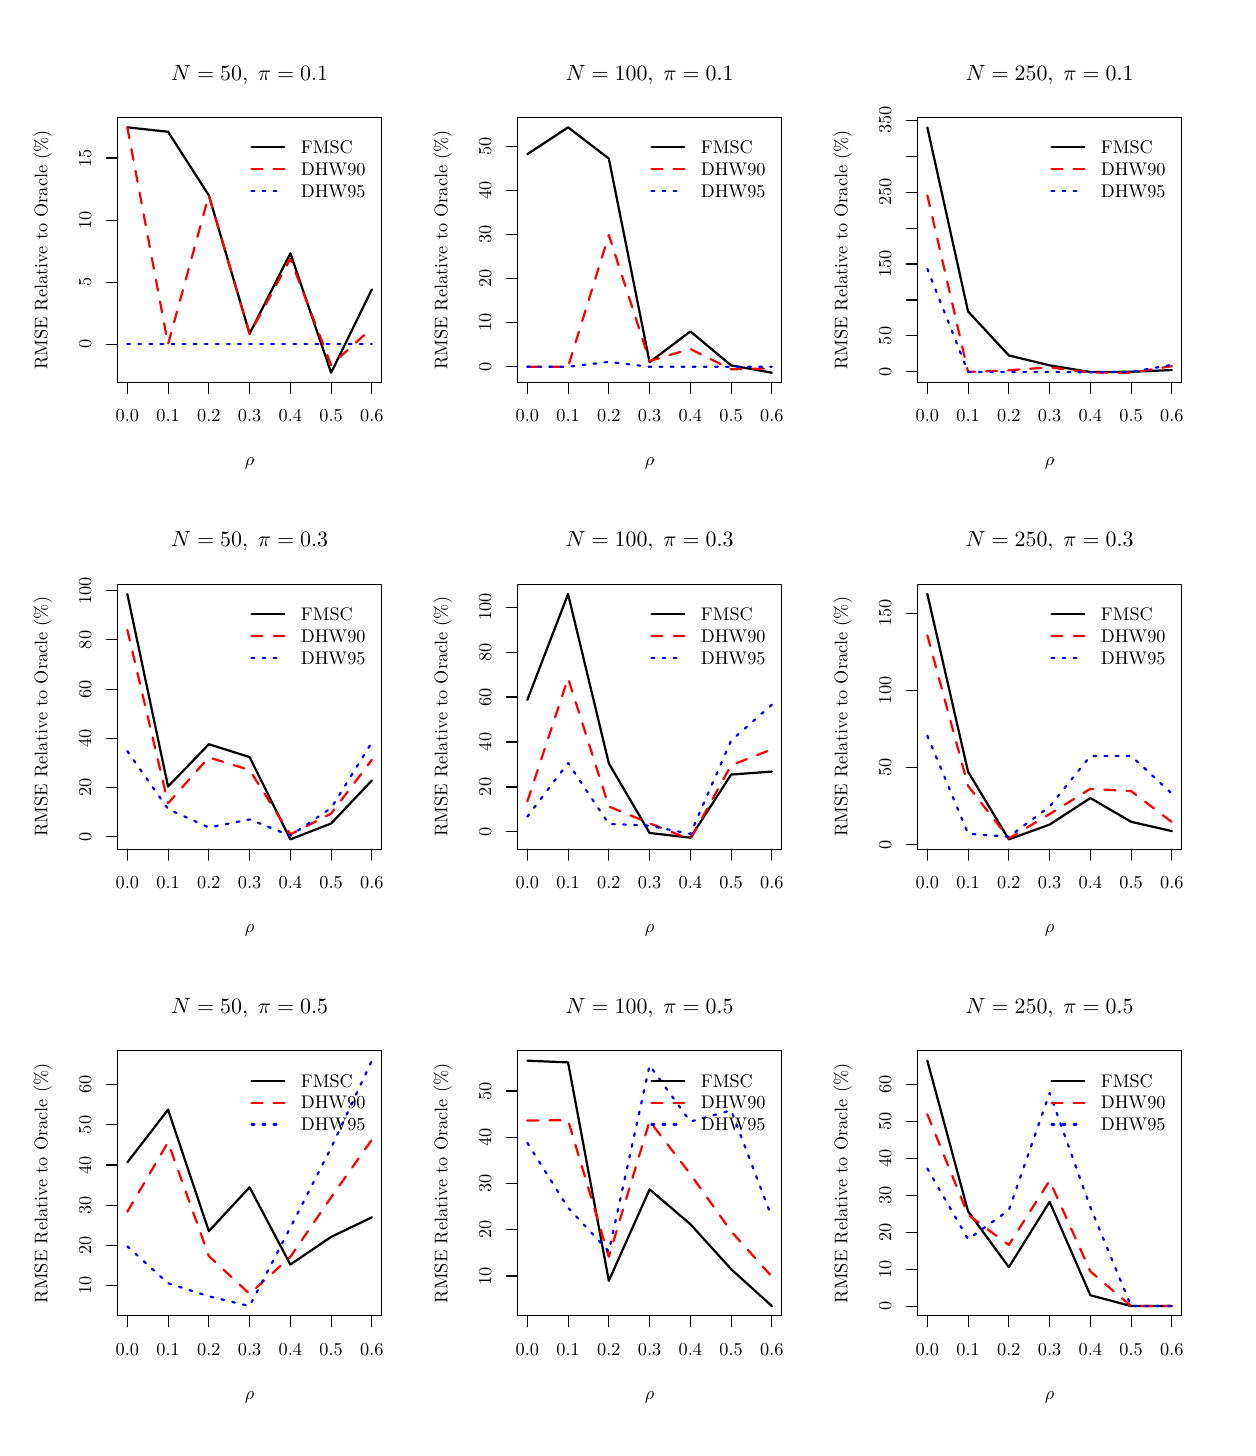
\begin{tikzpicture}[x=1pt,y=1pt]
\definecolor[named]{fillColor}{rgb}{1.00,1.00,1.00}
\path[use as bounding box,fill=fillColor,fill opacity=0.00] (0,0) rectangle (433.62,505.89);
\begin{scope}
\path[clip] ( 32.47,377.65) rectangle (127.91,473.42);
\definecolor[named]{drawColor}{rgb}{0.00,0.00,0.00}

\path[draw=drawColor,line width= 0.8pt,line join=round,line cap=round] ( 36.01,469.87) --
	( 50.73,468.26) --
	( 65.46,445.32) --
	( 80.19,395.31) --
	( 94.92,424.35) --
	(109.65,381.20) --
	(124.37,411.31);
\end{scope}
\begin{scope}
\path[clip] (  0.00,  0.00) rectangle (433.62,505.89);
\definecolor[named]{drawColor}{rgb}{0.00,0.00,0.00}

\path[draw=drawColor,line width= 0.4pt,line join=round,line cap=round] ( 36.01,377.65) -- (124.37,377.65);

\path[draw=drawColor,line width= 0.4pt,line join=round,line cap=round] ( 36.01,377.65) -- ( 36.01,373.69);

\path[draw=drawColor,line width= 0.4pt,line join=round,line cap=round] ( 50.73,377.65) -- ( 50.73,373.69);

\path[draw=drawColor,line width= 0.4pt,line join=round,line cap=round] ( 65.46,377.65) -- ( 65.46,373.69);

\path[draw=drawColor,line width= 0.4pt,line join=round,line cap=round] ( 80.19,377.65) -- ( 80.19,373.69);

\path[draw=drawColor,line width= 0.4pt,line join=round,line cap=round] ( 94.92,377.65) -- ( 94.92,373.69);

\path[draw=drawColor,line width= 0.4pt,line join=round,line cap=round] (109.65,377.65) -- (109.65,373.69);

\path[draw=drawColor,line width= 0.4pt,line join=round,line cap=round] (124.37,377.65) -- (124.37,373.69);

\node[text=drawColor,anchor=base,inner sep=0pt, outer sep=0pt, scale=  0.66] at ( 36.01,363.40) {0.0};

\node[text=drawColor,anchor=base,inner sep=0pt, outer sep=0pt, scale=  0.66] at ( 50.73,363.40) {0.1};

\node[text=drawColor,anchor=base,inner sep=0pt, outer sep=0pt, scale=  0.66] at ( 65.46,363.40) {0.2};

\node[text=drawColor,anchor=base,inner sep=0pt, outer sep=0pt, scale=  0.66] at ( 80.19,363.40) {0.3};

\node[text=drawColor,anchor=base,inner sep=0pt, outer sep=0pt, scale=  0.66] at ( 94.92,363.40) {0.4};

\node[text=drawColor,anchor=base,inner sep=0pt, outer sep=0pt, scale=  0.66] at (109.65,363.40) {0.5};

\node[text=drawColor,anchor=base,inner sep=0pt, outer sep=0pt, scale=  0.66] at (124.37,363.40) {0.6};

\path[draw=drawColor,line width= 0.4pt,line join=round,line cap=round] ( 32.47,391.50) -- ( 32.47,458.79);

\path[draw=drawColor,line width= 0.4pt,line join=round,line cap=round] ( 32.47,391.50) -- ( 28.51,391.50);

\path[draw=drawColor,line width= 0.4pt,line join=round,line cap=round] ( 32.47,413.93) -- ( 28.51,413.93);

\path[draw=drawColor,line width= 0.4pt,line join=round,line cap=round] ( 32.47,436.36) -- ( 28.51,436.36);

\path[draw=drawColor,line width= 0.4pt,line join=round,line cap=round] ( 32.47,458.79) -- ( 28.51,458.79);

\node[text=drawColor,rotate= 90.00,anchor=base,inner sep=0pt, outer sep=0pt, scale=  0.66] at ( 22.97,391.50) {0};

\node[text=drawColor,rotate= 90.00,anchor=base,inner sep=0pt, outer sep=0pt, scale=  0.66] at ( 22.97,413.93) {5};

\node[text=drawColor,rotate= 90.00,anchor=base,inner sep=0pt, outer sep=0pt, scale=  0.66] at ( 22.97,436.36) {10};

\node[text=drawColor,rotate= 90.00,anchor=base,inner sep=0pt, outer sep=0pt, scale=  0.66] at ( 22.97,458.79) {15};

\path[draw=drawColor,line width= 0.4pt,line join=round,line cap=round] ( 32.47,377.65) --
	(127.91,377.65) --
	(127.91,473.42) --
	( 32.47,473.42) --
	( 32.47,377.65);
\end{scope}
\begin{scope}
\path[clip] (  0.00,337.26) rectangle (144.54,505.89);
\definecolor[named]{drawColor}{rgb}{0.00,0.00,0.00}

\node[text=drawColor,anchor=base,inner sep=0pt, outer sep=0pt, scale=  0.79] at ( 80.19,486.92) {\bfseries $N=50, \;\pi=0.1$};

\node[text=drawColor,anchor=base,inner sep=0pt, outer sep=0pt, scale=  0.66] at ( 80.19,347.56) {$\rho$};

\node[text=drawColor,rotate= 90.00,anchor=base,inner sep=0pt, outer sep=0pt, scale=  0.66] at (  7.13,425.53) {RMSE Relative to Oracle (\%)};
\end{scope}
\begin{scope}
\path[clip] ( 32.47,377.65) rectangle (127.91,473.42);
\definecolor[named]{drawColor}{rgb}{1.00,0.00,0.00}

\path[draw=drawColor,line width= 0.8pt,dash pattern=on 4pt off 4pt ,line join=round,line cap=round] ( 36.01,469.87) --
	( 50.73,391.50) --
	( 65.46,445.32) --
	( 80.19,395.14) --
	( 94.92,422.38) --
	(109.65,383.99) --
	(124.37,397.30);
\definecolor[named]{drawColor}{rgb}{0.00,0.00,1.00}

\path[draw=drawColor,line width= 0.8pt,dash pattern=on 1pt off 3pt ,line join=round,line cap=round] ( 36.01,391.50) --
	( 50.73,391.50) --
	( 65.46,391.50) --
	( 80.19,391.50) --
	( 94.92,391.50) --
	(109.65,391.50) --
	(124.37,391.50);
\definecolor[named]{drawColor}{rgb}{0.00,0.00,0.00}

\path[draw=drawColor,line width= 0.8pt,line join=round,line cap=round] ( 80.89,462.63) -- ( 92.77,462.63);
\definecolor[named]{drawColor}{rgb}{1.00,0.00,0.00}

\path[draw=drawColor,line width= 0.8pt,dash pattern=on 4pt off 4pt ,line join=round,line cap=round] ( 80.89,454.71) -- ( 92.77,454.71);
\definecolor[named]{drawColor}{rgb}{0.00,0.00,1.00}

\path[draw=drawColor,line width= 0.8pt,dash pattern=on 1pt off 3pt ,line join=round,line cap=round] ( 80.89,446.79) -- ( 92.77,446.79);
\definecolor[named]{drawColor}{rgb}{0.00,0.00,0.00}

\node[text=drawColor,anchor=base west,inner sep=0pt, outer sep=0pt, scale=  0.66] at ( 98.71,460.35) {FMSC};

\node[text=drawColor,anchor=base west,inner sep=0pt, outer sep=0pt, scale=  0.66] at ( 98.71,452.43) {DHW90};

\node[text=drawColor,anchor=base west,inner sep=0pt, outer sep=0pt, scale=  0.66] at ( 98.71,444.51) {DHW95};
\end{scope}
\begin{scope}
\path[clip] (177.01,377.65) rectangle (272.45,473.42);
\definecolor[named]{drawColor}{rgb}{0.00,0.00,0.00}

\path[draw=drawColor,line width= 0.8pt,line join=round,line cap=round] (180.55,460.16) --
	(195.27,469.87) --
	(210.00,458.57) --
	(224.73,385.01) --
	(239.46,396.13) --
	(254.19,383.85) --
	(268.91,381.20);
\end{scope}
\begin{scope}
\path[clip] (  0.00,  0.00) rectangle (433.62,505.89);
\definecolor[named]{drawColor}{rgb}{0.00,0.00,0.00}

\path[draw=drawColor,line width= 0.4pt,line join=round,line cap=round] (180.55,377.65) -- (268.91,377.65);

\path[draw=drawColor,line width= 0.4pt,line join=round,line cap=round] (180.55,377.65) -- (180.55,373.69);

\path[draw=drawColor,line width= 0.4pt,line join=round,line cap=round] (195.27,377.65) -- (195.27,373.69);

\path[draw=drawColor,line width= 0.4pt,line join=round,line cap=round] (210.00,377.65) -- (210.00,373.69);

\path[draw=drawColor,line width= 0.4pt,line join=round,line cap=round] (224.73,377.65) -- (224.73,373.69);

\path[draw=drawColor,line width= 0.4pt,line join=round,line cap=round] (239.46,377.65) -- (239.46,373.69);

\path[draw=drawColor,line width= 0.4pt,line join=round,line cap=round] (254.19,377.65) -- (254.19,373.69);

\path[draw=drawColor,line width= 0.4pt,line join=round,line cap=round] (268.91,377.65) -- (268.91,373.69);

\node[text=drawColor,anchor=base,inner sep=0pt, outer sep=0pt, scale=  0.66] at (180.55,363.40) {0.0};

\node[text=drawColor,anchor=base,inner sep=0pt, outer sep=0pt, scale=  0.66] at (195.27,363.40) {0.1};

\node[text=drawColor,anchor=base,inner sep=0pt, outer sep=0pt, scale=  0.66] at (210.00,363.40) {0.2};

\node[text=drawColor,anchor=base,inner sep=0pt, outer sep=0pt, scale=  0.66] at (224.73,363.40) {0.3};

\node[text=drawColor,anchor=base,inner sep=0pt, outer sep=0pt, scale=  0.66] at (239.46,363.40) {0.4};

\node[text=drawColor,anchor=base,inner sep=0pt, outer sep=0pt, scale=  0.66] at (254.19,363.40) {0.5};

\node[text=drawColor,anchor=base,inner sep=0pt, outer sep=0pt, scale=  0.66] at (268.91,363.40) {0.6};

\path[draw=drawColor,line width= 0.4pt,line join=round,line cap=round] (177.01,383.35) -- (177.01,462.97);

\path[draw=drawColor,line width= 0.4pt,line join=round,line cap=round] (177.01,383.35) -- (173.05,383.35);

\path[draw=drawColor,line width= 0.4pt,line join=round,line cap=round] (177.01,399.27) -- (173.05,399.27);

\path[draw=drawColor,line width= 0.4pt,line join=round,line cap=round] (177.01,415.20) -- (173.05,415.20);

\path[draw=drawColor,line width= 0.4pt,line join=round,line cap=round] (177.01,431.12) -- (173.05,431.12);

\path[draw=drawColor,line width= 0.4pt,line join=round,line cap=round] (177.01,447.05) -- (173.05,447.05);

\path[draw=drawColor,line width= 0.4pt,line join=round,line cap=round] (177.01,462.97) -- (173.05,462.97);

\node[text=drawColor,rotate= 90.00,anchor=base,inner sep=0pt, outer sep=0pt, scale=  0.66] at (167.51,383.35) {0};

\node[text=drawColor,rotate= 90.00,anchor=base,inner sep=0pt, outer sep=0pt, scale=  0.66] at (167.51,399.27) {10};

\node[text=drawColor,rotate= 90.00,anchor=base,inner sep=0pt, outer sep=0pt, scale=  0.66] at (167.51,415.20) {20};

\node[text=drawColor,rotate= 90.00,anchor=base,inner sep=0pt, outer sep=0pt, scale=  0.66] at (167.51,431.12) {30};

\node[text=drawColor,rotate= 90.00,anchor=base,inner sep=0pt, outer sep=0pt, scale=  0.66] at (167.51,447.05) {40};

\node[text=drawColor,rotate= 90.00,anchor=base,inner sep=0pt, outer sep=0pt, scale=  0.66] at (167.51,462.97) {50};

\path[draw=drawColor,line width= 0.4pt,line join=round,line cap=round] (177.01,377.65) --
	(272.45,377.65) --
	(272.45,473.42) --
	(177.01,473.42) --
	(177.01,377.65);
\end{scope}
\begin{scope}
\path[clip] (144.54,337.26) rectangle (289.08,505.89);
\definecolor[named]{drawColor}{rgb}{0.00,0.00,0.00}

\node[text=drawColor,anchor=base,inner sep=0pt, outer sep=0pt, scale=  0.79] at (224.73,486.92) {\bfseries $N=100, \;\pi=0.1$};

\node[text=drawColor,anchor=base,inner sep=0pt, outer sep=0pt, scale=  0.66] at (224.73,347.56) {$\rho$};

\node[text=drawColor,rotate= 90.00,anchor=base,inner sep=0pt, outer sep=0pt, scale=  0.66] at (151.67,425.53) {RMSE Relative to Oracle (\%)};
\end{scope}
\begin{scope}
\path[clip] (177.01,377.65) rectangle (272.45,473.42);
\definecolor[named]{drawColor}{rgb}{1.00,0.00,0.00}

\path[draw=drawColor,line width= 0.8pt,dash pattern=on 4pt off 4pt ,line join=round,line cap=round] (180.55,383.35) --
	(195.27,383.35) --
	(210.00,430.97) --
	(224.73,385.44) --
	(239.46,389.78) --
	(254.19,382.44) --
	(268.91,382.80);
\definecolor[named]{drawColor}{rgb}{0.00,0.00,1.00}

\path[draw=drawColor,line width= 0.8pt,dash pattern=on 1pt off 3pt ,line join=round,line cap=round] (180.55,383.35) --
	(195.27,383.35) --
	(210.00,385.12) --
	(224.73,383.35) --
	(239.46,383.35) --
	(254.19,383.35) --
	(268.91,383.35);
\definecolor[named]{drawColor}{rgb}{0.00,0.00,0.00}

\path[draw=drawColor,line width= 0.8pt,line join=round,line cap=round] (225.43,462.63) -- (237.31,462.63);
\definecolor[named]{drawColor}{rgb}{1.00,0.00,0.00}

\path[draw=drawColor,line width= 0.8pt,dash pattern=on 4pt off 4pt ,line join=round,line cap=round] (225.43,454.71) -- (237.31,454.71);
\definecolor[named]{drawColor}{rgb}{0.00,0.00,1.00}

\path[draw=drawColor,line width= 0.8pt,dash pattern=on 1pt off 3pt ,line join=round,line cap=round] (225.43,446.79) -- (237.31,446.79);
\definecolor[named]{drawColor}{rgb}{0.00,0.00,0.00}

\node[text=drawColor,anchor=base west,inner sep=0pt, outer sep=0pt, scale=  0.66] at (243.25,460.35) {FMSC};

\node[text=drawColor,anchor=base west,inner sep=0pt, outer sep=0pt, scale=  0.66] at (243.25,452.43) {DHW90};

\node[text=drawColor,anchor=base west,inner sep=0pt, outer sep=0pt, scale=  0.66] at (243.25,444.51) {DHW95};
\end{scope}
\begin{scope}
\path[clip] (321.55,377.65) rectangle (416.99,473.42);
\definecolor[named]{drawColor}{rgb}{0.00,0.00,0.00}

\path[draw=drawColor,line width= 0.8pt,line join=round,line cap=round] (325.09,469.87) --
	(339.81,403.33) --
	(354.54,387.44) --
	(369.27,383.87) --
	(384.00,381.45) --
	(398.73,381.54) --
	(413.45,382.17);
\end{scope}
\begin{scope}
\path[clip] (  0.00,  0.00) rectangle (433.62,505.89);
\definecolor[named]{drawColor}{rgb}{0.00,0.00,0.00}

\path[draw=drawColor,line width= 0.4pt,line join=round,line cap=round] (325.09,377.65) -- (413.45,377.65);

\path[draw=drawColor,line width= 0.4pt,line join=round,line cap=round] (325.09,377.65) -- (325.09,373.69);

\path[draw=drawColor,line width= 0.4pt,line join=round,line cap=round] (339.81,377.65) -- (339.81,373.69);

\path[draw=drawColor,line width= 0.4pt,line join=round,line cap=round] (354.54,377.65) -- (354.54,373.69);

\path[draw=drawColor,line width= 0.4pt,line join=round,line cap=round] (369.27,377.65) -- (369.27,373.69);

\path[draw=drawColor,line width= 0.4pt,line join=round,line cap=round] (384.00,377.65) -- (384.00,373.69);

\path[draw=drawColor,line width= 0.4pt,line join=round,line cap=round] (398.73,377.65) -- (398.73,373.69);

\path[draw=drawColor,line width= 0.4pt,line join=round,line cap=round] (413.45,377.65) -- (413.45,373.69);

\node[text=drawColor,anchor=base,inner sep=0pt, outer sep=0pt, scale=  0.66] at (325.09,363.40) {0.0};

\node[text=drawColor,anchor=base,inner sep=0pt, outer sep=0pt, scale=  0.66] at (339.81,363.40) {0.1};

\node[text=drawColor,anchor=base,inner sep=0pt, outer sep=0pt, scale=  0.66] at (354.54,363.40) {0.2};

\node[text=drawColor,anchor=base,inner sep=0pt, outer sep=0pt, scale=  0.66] at (369.27,363.40) {0.3};

\node[text=drawColor,anchor=base,inner sep=0pt, outer sep=0pt, scale=  0.66] at (384.00,363.40) {0.4};

\node[text=drawColor,anchor=base,inner sep=0pt, outer sep=0pt, scale=  0.66] at (398.73,363.40) {0.5};

\node[text=drawColor,anchor=base,inner sep=0pt, outer sep=0pt, scale=  0.66] at (413.45,363.40) {0.6};

\path[draw=drawColor,line width= 0.4pt,line join=round,line cap=round] (321.55,381.49) -- (321.55,472.45);

\path[draw=drawColor,line width= 0.4pt,line join=round,line cap=round] (321.55,381.49) -- (317.59,381.49);

\path[draw=drawColor,line width= 0.4pt,line join=round,line cap=round] (321.55,394.49) -- (317.59,394.49);

\path[draw=drawColor,line width= 0.4pt,line join=round,line cap=round] (321.55,407.48) -- (317.59,407.48);

\path[draw=drawColor,line width= 0.4pt,line join=round,line cap=round] (321.55,420.47) -- (317.59,420.47);

\path[draw=drawColor,line width= 0.4pt,line join=round,line cap=round] (321.55,433.47) -- (317.59,433.47);

\path[draw=drawColor,line width= 0.4pt,line join=round,line cap=round] (321.55,446.46) -- (317.59,446.46);

\path[draw=drawColor,line width= 0.4pt,line join=round,line cap=round] (321.55,459.45) -- (317.59,459.45);

\path[draw=drawColor,line width= 0.4pt,line join=round,line cap=round] (321.55,472.45) -- (317.59,472.45);

\node[text=drawColor,rotate= 90.00,anchor=base,inner sep=0pt, outer sep=0pt, scale=  0.66] at (312.05,381.49) {0};

\node[text=drawColor,rotate= 90.00,anchor=base,inner sep=0pt, outer sep=0pt, scale=  0.66] at (312.05,394.49) {50};

\node[text=drawColor,rotate= 90.00,anchor=base,inner sep=0pt, outer sep=0pt, scale=  0.66] at (312.05,420.47) {150};

\node[text=drawColor,rotate= 90.00,anchor=base,inner sep=0pt, outer sep=0pt, scale=  0.66] at (312.05,446.46) {250};

\node[text=drawColor,rotate= 90.00,anchor=base,inner sep=0pt, outer sep=0pt, scale=  0.66] at (312.05,472.45) {350};

\path[draw=drawColor,line width= 0.4pt,line join=round,line cap=round] (321.55,377.65) --
	(416.99,377.65) --
	(416.99,473.42) --
	(321.55,473.42) --
	(321.55,377.65);
\end{scope}
\begin{scope}
\path[clip] (289.08,337.26) rectangle (433.62,505.89);
\definecolor[named]{drawColor}{rgb}{0.00,0.00,0.00}

\node[text=drawColor,anchor=base,inner sep=0pt, outer sep=0pt, scale=  0.79] at (369.27,486.92) {\bfseries $N=250, \;\pi=0.1$};

\node[text=drawColor,anchor=base,inner sep=0pt, outer sep=0pt, scale=  0.66] at (369.27,347.56) {$\rho$};

\node[text=drawColor,rotate= 90.00,anchor=base,inner sep=0pt, outer sep=0pt, scale=  0.66] at (296.21,425.53) {RMSE Relative to Oracle (\%)};
\end{scope}
\begin{scope}
\path[clip] (321.55,377.65) rectangle (416.99,473.42);
\definecolor[named]{drawColor}{rgb}{1.00,0.00,0.00}

\path[draw=drawColor,line width= 0.8pt,dash pattern=on 4pt off 4pt ,line join=round,line cap=round] (325.09,445.30) --
	(339.81,381.49) --
	(354.54,382.08) --
	(369.27,383.15) --
	(384.00,381.25) --
	(398.73,381.20) --
	(413.45,383.57);
\definecolor[named]{drawColor}{rgb}{0.00,0.00,1.00}

\path[draw=drawColor,line width= 0.8pt,dash pattern=on 1pt off 3pt ,line join=round,line cap=round] (325.09,418.73) --
	(339.81,381.49) --
	(354.54,381.49) --
	(369.27,381.49) --
	(384.00,381.37) --
	(398.73,381.49) --
	(413.45,384.04);
\definecolor[named]{drawColor}{rgb}{0.00,0.00,0.00}

\path[draw=drawColor,line width= 0.8pt,line join=round,line cap=round] (369.97,462.63) -- (381.85,462.63);
\definecolor[named]{drawColor}{rgb}{1.00,0.00,0.00}

\path[draw=drawColor,line width= 0.8pt,dash pattern=on 4pt off 4pt ,line join=round,line cap=round] (369.97,454.71) -- (381.85,454.71);
\definecolor[named]{drawColor}{rgb}{0.00,0.00,1.00}

\path[draw=drawColor,line width= 0.8pt,dash pattern=on 1pt off 3pt ,line join=round,line cap=round] (369.97,446.79) -- (381.85,446.79);
\definecolor[named]{drawColor}{rgb}{0.00,0.00,0.00}

\node[text=drawColor,anchor=base west,inner sep=0pt, outer sep=0pt, scale=  0.66] at (387.79,460.35) {FMSC};

\node[text=drawColor,anchor=base west,inner sep=0pt, outer sep=0pt, scale=  0.66] at (387.79,452.43) {DHW90};

\node[text=drawColor,anchor=base west,inner sep=0pt, outer sep=0pt, scale=  0.66] at (387.79,444.51) {DHW95};
\end{scope}
\begin{scope}
\path[clip] ( 32.47,209.02) rectangle (127.91,304.79);
\definecolor[named]{drawColor}{rgb}{0.00,0.00,0.00}

\path[draw=drawColor,line width= 0.8pt,line join=round,line cap=round] ( 36.01,301.24) --
	( 50.73,231.68) --
	( 65.46,246.96) --
	( 80.19,242.32) --
	( 94.92,212.57) --
	(109.65,218.32) --
	(124.37,233.85);
\end{scope}
\begin{scope}
\path[clip] (  0.00,  0.00) rectangle (433.62,505.89);
\definecolor[named]{drawColor}{rgb}{0.00,0.00,0.00}

\path[draw=drawColor,line width= 0.4pt,line join=round,line cap=round] ( 36.01,209.02) -- (124.37,209.02);

\path[draw=drawColor,line width= 0.4pt,line join=round,line cap=round] ( 36.01,209.02) -- ( 36.01,205.06);

\path[draw=drawColor,line width= 0.4pt,line join=round,line cap=round] ( 50.73,209.02) -- ( 50.73,205.06);

\path[draw=drawColor,line width= 0.4pt,line join=round,line cap=round] ( 65.46,209.02) -- ( 65.46,205.06);

\path[draw=drawColor,line width= 0.4pt,line join=round,line cap=round] ( 80.19,209.02) -- ( 80.19,205.06);

\path[draw=drawColor,line width= 0.4pt,line join=round,line cap=round] ( 94.92,209.02) -- ( 94.92,205.06);

\path[draw=drawColor,line width= 0.4pt,line join=round,line cap=round] (109.65,209.02) -- (109.65,205.06);

\path[draw=drawColor,line width= 0.4pt,line join=round,line cap=round] (124.37,209.02) -- (124.37,205.06);

\node[text=drawColor,anchor=base,inner sep=0pt, outer sep=0pt, scale=  0.66] at ( 36.01,194.77) {0.0};

\node[text=drawColor,anchor=base,inner sep=0pt, outer sep=0pt, scale=  0.66] at ( 50.73,194.77) {0.1};

\node[text=drawColor,anchor=base,inner sep=0pt, outer sep=0pt, scale=  0.66] at ( 65.46,194.77) {0.2};

\node[text=drawColor,anchor=base,inner sep=0pt, outer sep=0pt, scale=  0.66] at ( 80.19,194.77) {0.3};

\node[text=drawColor,anchor=base,inner sep=0pt, outer sep=0pt, scale=  0.66] at ( 94.92,194.77) {0.4};

\node[text=drawColor,anchor=base,inner sep=0pt, outer sep=0pt, scale=  0.66] at (109.65,194.77) {0.5};

\node[text=drawColor,anchor=base,inner sep=0pt, outer sep=0pt, scale=  0.66] at (124.37,194.77) {0.6};

\path[draw=drawColor,line width= 0.4pt,line join=round,line cap=round] ( 32.47,213.61) -- ( 32.47,302.41);

\path[draw=drawColor,line width= 0.4pt,line join=round,line cap=round] ( 32.47,213.61) -- ( 28.51,213.61);

\path[draw=drawColor,line width= 0.4pt,line join=round,line cap=round] ( 32.47,231.37) -- ( 28.51,231.37);

\path[draw=drawColor,line width= 0.4pt,line join=round,line cap=round] ( 32.47,249.13) -- ( 28.51,249.13);

\path[draw=drawColor,line width= 0.4pt,line join=round,line cap=round] ( 32.47,266.89) -- ( 28.51,266.89);

\path[draw=drawColor,line width= 0.4pt,line join=round,line cap=round] ( 32.47,284.65) -- ( 28.51,284.65);

\path[draw=drawColor,line width= 0.4pt,line join=round,line cap=round] ( 32.47,302.41) -- ( 28.51,302.41);

\node[text=drawColor,rotate= 90.00,anchor=base,inner sep=0pt, outer sep=0pt, scale=  0.66] at ( 22.97,213.61) {0};

\node[text=drawColor,rotate= 90.00,anchor=base,inner sep=0pt, outer sep=0pt, scale=  0.66] at ( 22.97,231.37) {20};

\node[text=drawColor,rotate= 90.00,anchor=base,inner sep=0pt, outer sep=0pt, scale=  0.66] at ( 22.97,249.13) {40};

\node[text=drawColor,rotate= 90.00,anchor=base,inner sep=0pt, outer sep=0pt, scale=  0.66] at ( 22.97,266.89) {60};

\node[text=drawColor,rotate= 90.00,anchor=base,inner sep=0pt, outer sep=0pt, scale=  0.66] at ( 22.97,284.65) {80};

\node[text=drawColor,rotate= 90.00,anchor=base,inner sep=0pt, outer sep=0pt, scale=  0.66] at ( 22.97,302.41) {100};

\path[draw=drawColor,line width= 0.4pt,line join=round,line cap=round] ( 32.47,209.02) --
	(127.91,209.02) --
	(127.91,304.79) --
	( 32.47,304.79) --
	( 32.47,209.02);
\end{scope}
\begin{scope}
\path[clip] (  0.00,168.63) rectangle (144.54,337.26);
\definecolor[named]{drawColor}{rgb}{0.00,0.00,0.00}

\node[text=drawColor,anchor=base,inner sep=0pt, outer sep=0pt, scale=  0.79] at ( 80.19,318.29) {\bfseries $N=50, \;\pi=0.3$};

\node[text=drawColor,anchor=base,inner sep=0pt, outer sep=0pt, scale=  0.66] at ( 80.19,178.93) {$\rho$};

\node[text=drawColor,rotate= 90.00,anchor=base,inner sep=0pt, outer sep=0pt, scale=  0.66] at (  7.13,256.90) {RMSE Relative to Oracle (\%)};
\end{scope}
\begin{scope}
\path[clip] ( 32.47,209.02) rectangle (127.91,304.79);
\definecolor[named]{drawColor}{rgb}{1.00,0.00,0.00}

\path[draw=drawColor,line width= 0.8pt,dash pattern=on 4pt off 4pt ,line join=round,line cap=round] ( 36.01,288.31) --
	( 50.73,225.62) --
	( 65.46,242.21) --
	( 80.19,237.64) --
	( 94.92,214.36) --
	(109.65,221.89) --
	(124.37,241.32);
\definecolor[named]{drawColor}{rgb}{0.00,0.00,1.00}

\path[draw=drawColor,line width= 0.8pt,dash pattern=on 1pt off 3pt ,line join=round,line cap=round] ( 36.01,244.47) --
	( 50.73,223.54) --
	( 65.46,216.87) --
	( 80.19,219.79) --
	( 94.92,213.90) --
	(109.65,223.89) --
	(124.37,247.63);
\definecolor[named]{drawColor}{rgb}{0.00,0.00,0.00}

\path[draw=drawColor,line width= 0.8pt,line join=round,line cap=round] ( 80.89,294.00) -- ( 92.77,294.00);
\definecolor[named]{drawColor}{rgb}{1.00,0.00,0.00}

\path[draw=drawColor,line width= 0.8pt,dash pattern=on 4pt off 4pt ,line join=round,line cap=round] ( 80.89,286.08) -- ( 92.77,286.08);
\definecolor[named]{drawColor}{rgb}{0.00,0.00,1.00}

\path[draw=drawColor,line width= 0.8pt,dash pattern=on 1pt off 3pt ,line join=round,line cap=round] ( 80.89,278.16) -- ( 92.77,278.16);
\definecolor[named]{drawColor}{rgb}{0.00,0.00,0.00}

\node[text=drawColor,anchor=base west,inner sep=0pt, outer sep=0pt, scale=  0.66] at ( 98.71,291.72) {FMSC};

\node[text=drawColor,anchor=base west,inner sep=0pt, outer sep=0pt, scale=  0.66] at ( 98.71,283.80) {DHW90};

\node[text=drawColor,anchor=base west,inner sep=0pt, outer sep=0pt, scale=  0.66] at ( 98.71,275.88) {DHW95};
\end{scope}
\begin{scope}
\path[clip] (177.01,209.02) rectangle (272.45,304.79);
\definecolor[named]{drawColor}{rgb}{0.00,0.00,0.00}

\path[draw=drawColor,line width= 0.8pt,line join=round,line cap=round] (180.55,262.98) --
	(195.27,301.24) --
	(210.00,240.04) --
	(224.73,214.89) --
	(239.46,213.19) --
	(254.19,236.00) --
	(268.91,237.07);
\end{scope}
\begin{scope}
\path[clip] (  0.00,  0.00) rectangle (433.62,505.89);
\definecolor[named]{drawColor}{rgb}{0.00,0.00,0.00}

\path[draw=drawColor,line width= 0.4pt,line join=round,line cap=round] (180.55,209.02) -- (268.91,209.02);

\path[draw=drawColor,line width= 0.4pt,line join=round,line cap=round] (180.55,209.02) -- (180.55,205.06);

\path[draw=drawColor,line width= 0.4pt,line join=round,line cap=round] (195.27,209.02) -- (195.27,205.06);

\path[draw=drawColor,line width= 0.4pt,line join=round,line cap=round] (210.00,209.02) -- (210.00,205.06);

\path[draw=drawColor,line width= 0.4pt,line join=round,line cap=round] (224.73,209.02) -- (224.73,205.06);

\path[draw=drawColor,line width= 0.4pt,line join=round,line cap=round] (239.46,209.02) -- (239.46,205.06);

\path[draw=drawColor,line width= 0.4pt,line join=round,line cap=round] (254.19,209.02) -- (254.19,205.06);

\path[draw=drawColor,line width= 0.4pt,line join=round,line cap=round] (268.91,209.02) -- (268.91,205.06);

\node[text=drawColor,anchor=base,inner sep=0pt, outer sep=0pt, scale=  0.66] at (180.55,194.77) {0.0};

\node[text=drawColor,anchor=base,inner sep=0pt, outer sep=0pt, scale=  0.66] at (195.27,194.77) {0.1};

\node[text=drawColor,anchor=base,inner sep=0pt, outer sep=0pt, scale=  0.66] at (210.00,194.77) {0.2};

\node[text=drawColor,anchor=base,inner sep=0pt, outer sep=0pt, scale=  0.66] at (224.73,194.77) {0.3};

\node[text=drawColor,anchor=base,inner sep=0pt, outer sep=0pt, scale=  0.66] at (239.46,194.77) {0.4};

\node[text=drawColor,anchor=base,inner sep=0pt, outer sep=0pt, scale=  0.66] at (254.19,194.77) {0.5};

\node[text=drawColor,anchor=base,inner sep=0pt, outer sep=0pt, scale=  0.66] at (268.91,194.77) {0.6};

\path[draw=drawColor,line width= 0.4pt,line join=round,line cap=round] (177.01,215.27) -- (177.01,296.51);

\path[draw=drawColor,line width= 0.4pt,line join=round,line cap=round] (177.01,215.27) -- (173.05,215.27);

\path[draw=drawColor,line width= 0.4pt,line join=round,line cap=round] (177.01,231.52) -- (173.05,231.52);

\path[draw=drawColor,line width= 0.4pt,line join=round,line cap=round] (177.01,247.77) -- (173.05,247.77);

\path[draw=drawColor,line width= 0.4pt,line join=round,line cap=round] (177.01,264.02) -- (173.05,264.02);

\path[draw=drawColor,line width= 0.4pt,line join=round,line cap=round] (177.01,280.26) -- (173.05,280.26);

\path[draw=drawColor,line width= 0.4pt,line join=round,line cap=round] (177.01,296.51) -- (173.05,296.51);

\node[text=drawColor,rotate= 90.00,anchor=base,inner sep=0pt, outer sep=0pt, scale=  0.66] at (167.51,215.27) {0};

\node[text=drawColor,rotate= 90.00,anchor=base,inner sep=0pt, outer sep=0pt, scale=  0.66] at (167.51,231.52) {20};

\node[text=drawColor,rotate= 90.00,anchor=base,inner sep=0pt, outer sep=0pt, scale=  0.66] at (167.51,247.77) {40};

\node[text=drawColor,rotate= 90.00,anchor=base,inner sep=0pt, outer sep=0pt, scale=  0.66] at (167.51,264.02) {60};

\node[text=drawColor,rotate= 90.00,anchor=base,inner sep=0pt, outer sep=0pt, scale=  0.66] at (167.51,280.26) {80};

\node[text=drawColor,rotate= 90.00,anchor=base,inner sep=0pt, outer sep=0pt, scale=  0.66] at (167.51,296.51) {100};

\path[draw=drawColor,line width= 0.4pt,line join=round,line cap=round] (177.01,209.02) --
	(272.45,209.02) --
	(272.45,304.79) --
	(177.01,304.79) --
	(177.01,209.02);
\end{scope}
\begin{scope}
\path[clip] (144.54,168.63) rectangle (289.08,337.26);
\definecolor[named]{drawColor}{rgb}{0.00,0.00,0.00}

\node[text=drawColor,anchor=base,inner sep=0pt, outer sep=0pt, scale=  0.79] at (224.73,318.29) {\bfseries $N=100, \;\pi=0.3$};

\node[text=drawColor,anchor=base,inner sep=0pt, outer sep=0pt, scale=  0.66] at (224.73,178.93) {$\rho$};

\node[text=drawColor,rotate= 90.00,anchor=base,inner sep=0pt, outer sep=0pt, scale=  0.66] at (151.67,256.90) {RMSE Relative to Oracle (\%)};
\end{scope}
\begin{scope}
\path[clip] (177.01,209.02) rectangle (272.45,304.79);
\definecolor[named]{drawColor}{rgb}{1.00,0.00,0.00}

\path[draw=drawColor,line width= 0.8pt,dash pattern=on 4pt off 4pt ,line join=round,line cap=round] (180.55,226.30) --
	(195.27,270.83) --
	(210.00,224.46) --
	(224.73,218.40) --
	(239.46,212.57) --
	(254.19,239.38) --
	(268.91,245.10);
\definecolor[named]{drawColor}{rgb}{0.00,0.00,1.00}

\path[draw=drawColor,line width= 0.8pt,dash pattern=on 1pt off 3pt ,line join=round,line cap=round] (180.55,220.79) --
	(195.27,240.17) --
	(210.00,218.17) --
	(224.73,217.52) --
	(239.46,214.54) --
	(254.19,248.27) --
	(268.91,261.23);
\definecolor[named]{drawColor}{rgb}{0.00,0.00,0.00}

\path[draw=drawColor,line width= 0.8pt,line join=round,line cap=round] (225.43,294.00) -- (237.31,294.00);
\definecolor[named]{drawColor}{rgb}{1.00,0.00,0.00}

\path[draw=drawColor,line width= 0.8pt,dash pattern=on 4pt off 4pt ,line join=round,line cap=round] (225.43,286.08) -- (237.31,286.08);
\definecolor[named]{drawColor}{rgb}{0.00,0.00,1.00}

\path[draw=drawColor,line width= 0.8pt,dash pattern=on 1pt off 3pt ,line join=round,line cap=round] (225.43,278.16) -- (237.31,278.16);
\definecolor[named]{drawColor}{rgb}{0.00,0.00,0.00}

\node[text=drawColor,anchor=base west,inner sep=0pt, outer sep=0pt, scale=  0.66] at (243.25,291.72) {FMSC};

\node[text=drawColor,anchor=base west,inner sep=0pt, outer sep=0pt, scale=  0.66] at (243.25,283.80) {DHW90};

\node[text=drawColor,anchor=base west,inner sep=0pt, outer sep=0pt, scale=  0.66] at (243.25,275.88) {DHW95};
\end{scope}
\begin{scope}
\path[clip] (321.55,209.02) rectangle (416.99,304.79);
\definecolor[named]{drawColor}{rgb}{0.00,0.00,0.00}

\path[draw=drawColor,line width= 0.8pt,line join=round,line cap=round] (325.09,301.24) --
	(339.81,237.01) --
	(354.54,212.57) --
	(369.27,217.92) --
	(384.00,227.51) --
	(398.73,218.93) --
	(413.45,215.57);
\end{scope}
\begin{scope}
\path[clip] (  0.00,  0.00) rectangle (433.62,505.89);
\definecolor[named]{drawColor}{rgb}{0.00,0.00,0.00}

\path[draw=drawColor,line width= 0.4pt,line join=round,line cap=round] (325.09,209.02) -- (413.45,209.02);

\path[draw=drawColor,line width= 0.4pt,line join=round,line cap=round] (325.09,209.02) -- (325.09,205.06);

\path[draw=drawColor,line width= 0.4pt,line join=round,line cap=round] (339.81,209.02) -- (339.81,205.06);

\path[draw=drawColor,line width= 0.4pt,line join=round,line cap=round] (354.54,209.02) -- (354.54,205.06);

\path[draw=drawColor,line width= 0.4pt,line join=round,line cap=round] (369.27,209.02) -- (369.27,205.06);

\path[draw=drawColor,line width= 0.4pt,line join=round,line cap=round] (384.00,209.02) -- (384.00,205.06);

\path[draw=drawColor,line width= 0.4pt,line join=round,line cap=round] (398.73,209.02) -- (398.73,205.06);

\path[draw=drawColor,line width= 0.4pt,line join=round,line cap=round] (413.45,209.02) -- (413.45,205.06);

\node[text=drawColor,anchor=base,inner sep=0pt, outer sep=0pt, scale=  0.66] at (325.09,194.77) {0.0};

\node[text=drawColor,anchor=base,inner sep=0pt, outer sep=0pt, scale=  0.66] at (339.81,194.77) {0.1};

\node[text=drawColor,anchor=base,inner sep=0pt, outer sep=0pt, scale=  0.66] at (354.54,194.77) {0.2};

\node[text=drawColor,anchor=base,inner sep=0pt, outer sep=0pt, scale=  0.66] at (369.27,194.77) {0.3};

\node[text=drawColor,anchor=base,inner sep=0pt, outer sep=0pt, scale=  0.66] at (384.00,194.77) {0.4};

\node[text=drawColor,anchor=base,inner sep=0pt, outer sep=0pt, scale=  0.66] at (398.73,194.77) {0.5};

\node[text=drawColor,anchor=base,inner sep=0pt, outer sep=0pt, scale=  0.66] at (413.45,194.77) {0.6};

\path[draw=drawColor,line width= 0.4pt,line join=round,line cap=round] (321.55,210.72) -- (321.55,294.29);

\path[draw=drawColor,line width= 0.4pt,line join=round,line cap=round] (321.55,210.72) -- (317.59,210.72);

\path[draw=drawColor,line width= 0.4pt,line join=round,line cap=round] (321.55,238.57) -- (317.59,238.57);

\path[draw=drawColor,line width= 0.4pt,line join=round,line cap=round] (321.55,266.43) -- (317.59,266.43);

\path[draw=drawColor,line width= 0.4pt,line join=round,line cap=round] (321.55,294.29) -- (317.59,294.29);

\node[text=drawColor,rotate= 90.00,anchor=base,inner sep=0pt, outer sep=0pt, scale=  0.66] at (312.05,210.72) {0};

\node[text=drawColor,rotate= 90.00,anchor=base,inner sep=0pt, outer sep=0pt, scale=  0.66] at (312.05,238.57) {50};

\node[text=drawColor,rotate= 90.00,anchor=base,inner sep=0pt, outer sep=0pt, scale=  0.66] at (312.05,266.43) {100};

\node[text=drawColor,rotate= 90.00,anchor=base,inner sep=0pt, outer sep=0pt, scale=  0.66] at (312.05,294.29) {150};

\path[draw=drawColor,line width= 0.4pt,line join=round,line cap=round] (321.55,209.02) --
	(416.99,209.02) --
	(416.99,304.79) --
	(321.55,304.79) --
	(321.55,209.02);
\end{scope}
\begin{scope}
\path[clip] (289.08,168.63) rectangle (433.62,337.26);
\definecolor[named]{drawColor}{rgb}{0.00,0.00,0.00}

\node[text=drawColor,anchor=base,inner sep=0pt, outer sep=0pt, scale=  0.79] at (369.27,318.29) {\bfseries $N=250, \;\pi=0.3$};

\node[text=drawColor,anchor=base,inner sep=0pt, outer sep=0pt, scale=  0.66] at (369.27,178.93) {$\rho$};

\node[text=drawColor,rotate= 90.00,anchor=base,inner sep=0pt, outer sep=0pt, scale=  0.66] at (296.21,256.90) {RMSE Relative to Oracle (\%)};
\end{scope}
\begin{scope}
\path[clip] (321.55,209.02) rectangle (416.99,304.79);
\definecolor[named]{drawColor}{rgb}{1.00,0.00,0.00}

\path[draw=drawColor,line width= 0.8pt,dash pattern=on 4pt off 4pt ,line join=round,line cap=round] (325.09,286.34) --
	(339.81,231.89) --
	(354.54,212.91) --
	(369.27,221.72) --
	(384.00,230.84) --
	(398.73,230.02) --
	(413.45,218.83);
\definecolor[named]{drawColor}{rgb}{0.00,0.00,1.00}

\path[draw=drawColor,line width= 0.8pt,dash pattern=on 1pt off 3pt ,line join=round,line cap=round] (325.09,250.03) --
	(339.81,214.63) --
	(354.54,213.53) --
	(369.27,224.42) --
	(384.00,242.69) --
	(398.73,242.75) --
	(413.45,229.09);
\definecolor[named]{drawColor}{rgb}{0.00,0.00,0.00}

\path[draw=drawColor,line width= 0.8pt,line join=round,line cap=round] (369.97,294.00) -- (381.85,294.00);
\definecolor[named]{drawColor}{rgb}{1.00,0.00,0.00}

\path[draw=drawColor,line width= 0.8pt,dash pattern=on 4pt off 4pt ,line join=round,line cap=round] (369.97,286.08) -- (381.85,286.08);
\definecolor[named]{drawColor}{rgb}{0.00,0.00,1.00}

\path[draw=drawColor,line width= 0.8pt,dash pattern=on 1pt off 3pt ,line join=round,line cap=round] (369.97,278.16) -- (381.85,278.16);
\definecolor[named]{drawColor}{rgb}{0.00,0.00,0.00}

\node[text=drawColor,anchor=base west,inner sep=0pt, outer sep=0pt, scale=  0.66] at (387.79,291.72) {FMSC};

\node[text=drawColor,anchor=base west,inner sep=0pt, outer sep=0pt, scale=  0.66] at (387.79,283.80) {DHW90};

\node[text=drawColor,anchor=base west,inner sep=0pt, outer sep=0pt, scale=  0.66] at (387.79,275.88) {DHW95};
\end{scope}
\begin{scope}
\path[clip] ( 32.47, 40.39) rectangle (127.91,136.16);
\definecolor[named]{drawColor}{rgb}{0.00,0.00,0.00}

\path[draw=drawColor,line width= 0.8pt,line join=round,line cap=round] ( 36.01, 95.85) --
	( 50.73,114.93) --
	( 65.46, 71.00) --
	( 80.19, 86.87) --
	( 94.92, 58.95) --
	(109.65, 68.93) --
	(124.37, 76.01);
\end{scope}
\begin{scope}
\path[clip] (  0.00,  0.00) rectangle (433.62,505.89);
\definecolor[named]{drawColor}{rgb}{0.00,0.00,0.00}

\path[draw=drawColor,line width= 0.4pt,line join=round,line cap=round] ( 36.01, 40.39) -- (124.37, 40.39);

\path[draw=drawColor,line width= 0.4pt,line join=round,line cap=round] ( 36.01, 40.39) -- ( 36.01, 36.43);

\path[draw=drawColor,line width= 0.4pt,line join=round,line cap=round] ( 50.73, 40.39) -- ( 50.73, 36.43);

\path[draw=drawColor,line width= 0.4pt,line join=round,line cap=round] ( 65.46, 40.39) -- ( 65.46, 36.43);

\path[draw=drawColor,line width= 0.4pt,line join=round,line cap=round] ( 80.19, 40.39) -- ( 80.19, 36.43);

\path[draw=drawColor,line width= 0.4pt,line join=round,line cap=round] ( 94.92, 40.39) -- ( 94.92, 36.43);

\path[draw=drawColor,line width= 0.4pt,line join=round,line cap=round] (109.65, 40.39) -- (109.65, 36.43);

\path[draw=drawColor,line width= 0.4pt,line join=round,line cap=round] (124.37, 40.39) -- (124.37, 36.43);

\node[text=drawColor,anchor=base,inner sep=0pt, outer sep=0pt, scale=  0.66] at ( 36.01, 26.14) {0.0};

\node[text=drawColor,anchor=base,inner sep=0pt, outer sep=0pt, scale=  0.66] at ( 50.73, 26.14) {0.1};

\node[text=drawColor,anchor=base,inner sep=0pt, outer sep=0pt, scale=  0.66] at ( 65.46, 26.14) {0.2};

\node[text=drawColor,anchor=base,inner sep=0pt, outer sep=0pt, scale=  0.66] at ( 80.19, 26.14) {0.3};

\node[text=drawColor,anchor=base,inner sep=0pt, outer sep=0pt, scale=  0.66] at ( 94.92, 26.14) {0.4};

\node[text=drawColor,anchor=base,inner sep=0pt, outer sep=0pt, scale=  0.66] at (109.65, 26.14) {0.5};

\node[text=drawColor,anchor=base,inner sep=0pt, outer sep=0pt, scale=  0.66] at (124.37, 26.14) {0.6};

\path[draw=drawColor,line width= 0.4pt,line join=round,line cap=round] ( 32.47, 51.36) -- ( 32.47,123.92);

\path[draw=drawColor,line width= 0.4pt,line join=round,line cap=round] ( 32.47, 51.36) -- ( 28.51, 51.36);

\path[draw=drawColor,line width= 0.4pt,line join=round,line cap=round] ( 32.47, 65.87) -- ( 28.51, 65.87);

\path[draw=drawColor,line width= 0.4pt,line join=round,line cap=round] ( 32.47, 80.39) -- ( 28.51, 80.39);

\path[draw=drawColor,line width= 0.4pt,line join=round,line cap=round] ( 32.47, 94.90) -- ( 28.51, 94.90);

\path[draw=drawColor,line width= 0.4pt,line join=round,line cap=round] ( 32.47,109.41) -- ( 28.51,109.41);

\path[draw=drawColor,line width= 0.4pt,line join=round,line cap=round] ( 32.47,123.92) -- ( 28.51,123.92);

\node[text=drawColor,rotate= 90.00,anchor=base,inner sep=0pt, outer sep=0pt, scale=  0.66] at ( 22.97, 51.36) {10};

\node[text=drawColor,rotate= 90.00,anchor=base,inner sep=0pt, outer sep=0pt, scale=  0.66] at ( 22.97, 65.87) {20};

\node[text=drawColor,rotate= 90.00,anchor=base,inner sep=0pt, outer sep=0pt, scale=  0.66] at ( 22.97, 80.39) {30};

\node[text=drawColor,rotate= 90.00,anchor=base,inner sep=0pt, outer sep=0pt, scale=  0.66] at ( 22.97, 94.90) {40};

\node[text=drawColor,rotate= 90.00,anchor=base,inner sep=0pt, outer sep=0pt, scale=  0.66] at ( 22.97,109.41) {50};

\node[text=drawColor,rotate= 90.00,anchor=base,inner sep=0pt, outer sep=0pt, scale=  0.66] at ( 22.97,123.92) {60};

\path[draw=drawColor,line width= 0.4pt,line join=round,line cap=round] ( 32.47, 40.39) --
	(127.91, 40.39) --
	(127.91,136.16) --
	( 32.47,136.16) --
	( 32.47, 40.39);
\end{scope}
\begin{scope}
\path[clip] (  0.00,  0.00) rectangle (144.54,168.63);
\definecolor[named]{drawColor}{rgb}{0.00,0.00,0.00}

\node[text=drawColor,anchor=base,inner sep=0pt, outer sep=0pt, scale=  0.79] at ( 80.19,149.66) {\bfseries $N=50, \;\pi=0.5$};

\node[text=drawColor,anchor=base,inner sep=0pt, outer sep=0pt, scale=  0.66] at ( 80.19, 10.30) {$\rho$};

\node[text=drawColor,rotate= 90.00,anchor=base,inner sep=0pt, outer sep=0pt, scale=  0.66] at (  7.13, 88.27) {RMSE Relative to Oracle (\%)};
\end{scope}
\begin{scope}
\path[clip] ( 32.47, 40.39) rectangle (127.91,136.16);
\definecolor[named]{drawColor}{rgb}{1.00,0.00,0.00}

\path[draw=drawColor,line width= 0.8pt,dash pattern=on 4pt off 4pt ,line join=round,line cap=round] ( 36.01, 78.02) --
	( 50.73,103.12) --
	( 65.46, 62.02) --
	( 80.19, 48.35) --
	( 94.92, 61.70) --
	(109.65, 83.26) --
	(124.37,104.04);
\definecolor[named]{drawColor}{rgb}{0.00,0.00,1.00}

\path[draw=drawColor,line width= 0.8pt,dash pattern=on 1pt off 3pt ,line join=round,line cap=round] ( 36.01, 65.50) --
	( 50.73, 52.18) --
	( 65.46, 47.48) --
	( 80.19, 43.94) --
	( 94.92, 72.32) --
	(109.65,101.13) --
	(124.37,132.61);
\definecolor[named]{drawColor}{rgb}{0.00,0.00,0.00}

\path[draw=drawColor,line width= 0.8pt,line join=round,line cap=round] ( 80.89,125.37) -- ( 92.77,125.37);
\definecolor[named]{drawColor}{rgb}{1.00,0.00,0.00}

\path[draw=drawColor,line width= 0.8pt,dash pattern=on 4pt off 4pt ,line join=round,line cap=round] ( 80.89,117.45) -- ( 92.77,117.45);
\definecolor[named]{drawColor}{rgb}{0.00,0.00,1.00}

\path[draw=drawColor,line width= 0.8pt,dash pattern=on 1pt off 3pt ,line join=round,line cap=round] ( 80.89,109.53) -- ( 92.77,109.53);
\definecolor[named]{drawColor}{rgb}{0.00,0.00,0.00}

\node[text=drawColor,anchor=base west,inner sep=0pt, outer sep=0pt, scale=  0.66] at ( 98.71,123.09) {FMSC};

\node[text=drawColor,anchor=base west,inner sep=0pt, outer sep=0pt, scale=  0.66] at ( 98.71,115.17) {DHW90};

\node[text=drawColor,anchor=base west,inner sep=0pt, outer sep=0pt, scale=  0.66] at ( 98.71,107.25) {DHW95};
\end{scope}
\begin{scope}
\path[clip] (177.01, 40.39) rectangle (272.45,136.16);
\definecolor[named]{drawColor}{rgb}{0.00,0.00,0.00}

\path[draw=drawColor,line width= 0.8pt,line join=round,line cap=round] (180.55,132.61) --
	(195.27,131.99) --
	(210.00, 53.07) --
	(224.73, 86.11) --
	(239.46, 73.53) --
	(254.19, 57.28) --
	(268.91, 43.94);
\end{scope}
\begin{scope}
\path[clip] (  0.00,  0.00) rectangle (433.62,505.89);
\definecolor[named]{drawColor}{rgb}{0.00,0.00,0.00}

\path[draw=drawColor,line width= 0.4pt,line join=round,line cap=round] (180.55, 40.39) -- (268.91, 40.39);

\path[draw=drawColor,line width= 0.4pt,line join=round,line cap=round] (180.55, 40.39) -- (180.55, 36.43);

\path[draw=drawColor,line width= 0.4pt,line join=round,line cap=round] (195.27, 40.39) -- (195.27, 36.43);

\path[draw=drawColor,line width= 0.4pt,line join=round,line cap=round] (210.00, 40.39) -- (210.00, 36.43);

\path[draw=drawColor,line width= 0.4pt,line join=round,line cap=round] (224.73, 40.39) -- (224.73, 36.43);

\path[draw=drawColor,line width= 0.4pt,line join=round,line cap=round] (239.46, 40.39) -- (239.46, 36.43);

\path[draw=drawColor,line width= 0.4pt,line join=round,line cap=round] (254.19, 40.39) -- (254.19, 36.43);

\path[draw=drawColor,line width= 0.4pt,line join=round,line cap=round] (268.91, 40.39) -- (268.91, 36.43);

\node[text=drawColor,anchor=base,inner sep=0pt, outer sep=0pt, scale=  0.66] at (180.55, 26.14) {0.0};

\node[text=drawColor,anchor=base,inner sep=0pt, outer sep=0pt, scale=  0.66] at (195.27, 26.14) {0.1};

\node[text=drawColor,anchor=base,inner sep=0pt, outer sep=0pt, scale=  0.66] at (210.00, 26.14) {0.2};

\node[text=drawColor,anchor=base,inner sep=0pt, outer sep=0pt, scale=  0.66] at (224.73, 26.14) {0.3};

\node[text=drawColor,anchor=base,inner sep=0pt, outer sep=0pt, scale=  0.66] at (239.46, 26.14) {0.4};

\node[text=drawColor,anchor=base,inner sep=0pt, outer sep=0pt, scale=  0.66] at (254.19, 26.14) {0.5};

\node[text=drawColor,anchor=base,inner sep=0pt, outer sep=0pt, scale=  0.66] at (268.91, 26.14) {0.6};

\path[draw=drawColor,line width= 0.4pt,line join=round,line cap=round] (177.01, 54.79) -- (177.01,121.65);

\path[draw=drawColor,line width= 0.4pt,line join=round,line cap=round] (177.01, 54.79) -- (173.05, 54.79);

\path[draw=drawColor,line width= 0.4pt,line join=round,line cap=round] (177.01, 71.51) -- (173.05, 71.51);

\path[draw=drawColor,line width= 0.4pt,line join=round,line cap=round] (177.01, 88.22) -- (173.05, 88.22);

\path[draw=drawColor,line width= 0.4pt,line join=round,line cap=round] (177.01,104.93) -- (173.05,104.93);

\path[draw=drawColor,line width= 0.4pt,line join=round,line cap=round] (177.01,121.65) -- (173.05,121.65);

\node[text=drawColor,rotate= 90.00,anchor=base,inner sep=0pt, outer sep=0pt, scale=  0.66] at (167.51, 54.79) {10};

\node[text=drawColor,rotate= 90.00,anchor=base,inner sep=0pt, outer sep=0pt, scale=  0.66] at (167.51, 71.51) {20};

\node[text=drawColor,rotate= 90.00,anchor=base,inner sep=0pt, outer sep=0pt, scale=  0.66] at (167.51, 88.22) {30};

\node[text=drawColor,rotate= 90.00,anchor=base,inner sep=0pt, outer sep=0pt, scale=  0.66] at (167.51,104.93) {40};

\node[text=drawColor,rotate= 90.00,anchor=base,inner sep=0pt, outer sep=0pt, scale=  0.66] at (167.51,121.65) {50};

\path[draw=drawColor,line width= 0.4pt,line join=round,line cap=round] (177.01, 40.39) --
	(272.45, 40.39) --
	(272.45,136.16) --
	(177.01,136.16) --
	(177.01, 40.39);
\end{scope}
\begin{scope}
\path[clip] (144.54,  0.00) rectangle (289.08,168.63);
\definecolor[named]{drawColor}{rgb}{0.00,0.00,0.00}

\node[text=drawColor,anchor=base,inner sep=0pt, outer sep=0pt, scale=  0.79] at (224.73,149.66) {\bfseries $N=100, \;\pi=0.5$};

\node[text=drawColor,anchor=base,inner sep=0pt, outer sep=0pt, scale=  0.66] at (224.73, 10.30) {$\rho$};

\node[text=drawColor,rotate= 90.00,anchor=base,inner sep=0pt, outer sep=0pt, scale=  0.66] at (151.67, 88.27) {RMSE Relative to Oracle (\%)};
\end{scope}
\begin{scope}
\path[clip] (177.01, 40.39) rectangle (272.45,136.16);
\definecolor[named]{drawColor}{rgb}{1.00,0.00,0.00}

\path[draw=drawColor,line width= 0.8pt,dash pattern=on 4pt off 4pt ,line join=round,line cap=round] (180.55,110.96) --
	(195.27,111.12) --
	(210.00, 61.76) --
	(224.73,110.79) --
	(239.46, 91.63) --
	(254.19, 70.97) --
	(268.91, 54.57);
\definecolor[named]{drawColor}{rgb}{0.00,0.00,1.00}

\path[draw=drawColor,line width= 0.8pt,dash pattern=on 1pt off 3pt ,line join=round,line cap=round] (180.55,102.93) --
	(195.27, 79.48) --
	(210.00, 63.68) --
	(224.73,130.93) --
	(239.46,110.57) --
	(254.19,114.68) --
	(268.91, 76.04);
\definecolor[named]{drawColor}{rgb}{0.00,0.00,0.00}

\path[draw=drawColor,line width= 0.8pt,line join=round,line cap=round] (225.43,125.37) -- (237.31,125.37);
\definecolor[named]{drawColor}{rgb}{1.00,0.00,0.00}

\path[draw=drawColor,line width= 0.8pt,dash pattern=on 4pt off 4pt ,line join=round,line cap=round] (225.43,117.45) -- (237.31,117.45);
\definecolor[named]{drawColor}{rgb}{0.00,0.00,1.00}

\path[draw=drawColor,line width= 0.8pt,dash pattern=on 1pt off 3pt ,line join=round,line cap=round] (225.43,109.53) -- (237.31,109.53);
\definecolor[named]{drawColor}{rgb}{0.00,0.00,0.00}

\node[text=drawColor,anchor=base west,inner sep=0pt, outer sep=0pt, scale=  0.66] at (243.25,123.09) {FMSC};

\node[text=drawColor,anchor=base west,inner sep=0pt, outer sep=0pt, scale=  0.66] at (243.25,115.17) {DHW90};

\node[text=drawColor,anchor=base west,inner sep=0pt, outer sep=0pt, scale=  0.66] at (243.25,107.25) {DHW95};
\end{scope}
\begin{scope}
\path[clip] (321.55, 40.39) rectangle (416.99,136.16);
\definecolor[named]{drawColor}{rgb}{0.00,0.00,0.00}

\path[draw=drawColor,line width= 0.8pt,line join=round,line cap=round] (325.09,132.61) --
	(339.81, 78.16) --
	(354.54, 58.01) --
	(369.27, 81.62) --
	(384.00, 47.86) --
	(398.73, 43.94) --
	(413.45, 43.94);
\end{scope}
\begin{scope}
\path[clip] (  0.00,  0.00) rectangle (433.62,505.89);
\definecolor[named]{drawColor}{rgb}{0.00,0.00,0.00}

\path[draw=drawColor,line width= 0.4pt,line join=round,line cap=round] (325.09, 40.39) -- (413.45, 40.39);

\path[draw=drawColor,line width= 0.4pt,line join=round,line cap=round] (325.09, 40.39) -- (325.09, 36.43);

\path[draw=drawColor,line width= 0.4pt,line join=round,line cap=round] (339.81, 40.39) -- (339.81, 36.43);

\path[draw=drawColor,line width= 0.4pt,line join=round,line cap=round] (354.54, 40.39) -- (354.54, 36.43);

\path[draw=drawColor,line width= 0.4pt,line join=round,line cap=round] (369.27, 40.39) -- (369.27, 36.43);

\path[draw=drawColor,line width= 0.4pt,line join=round,line cap=round] (384.00, 40.39) -- (384.00, 36.43);

\path[draw=drawColor,line width= 0.4pt,line join=round,line cap=round] (398.73, 40.39) -- (398.73, 36.43);

\path[draw=drawColor,line width= 0.4pt,line join=round,line cap=round] (413.45, 40.39) -- (413.45, 36.43);

\node[text=drawColor,anchor=base,inner sep=0pt, outer sep=0pt, scale=  0.66] at (325.09, 26.14) {0.0};

\node[text=drawColor,anchor=base,inner sep=0pt, outer sep=0pt, scale=  0.66] at (339.81, 26.14) {0.1};

\node[text=drawColor,anchor=base,inner sep=0pt, outer sep=0pt, scale=  0.66] at (354.54, 26.14) {0.2};

\node[text=drawColor,anchor=base,inner sep=0pt, outer sep=0pt, scale=  0.66] at (369.27, 26.14) {0.3};

\node[text=drawColor,anchor=base,inner sep=0pt, outer sep=0pt, scale=  0.66] at (384.00, 26.14) {0.4};

\node[text=drawColor,anchor=base,inner sep=0pt, outer sep=0pt, scale=  0.66] at (398.73, 26.14) {0.5};

\node[text=drawColor,anchor=base,inner sep=0pt, outer sep=0pt, scale=  0.66] at (413.45, 26.14) {0.6};

\path[draw=drawColor,line width= 0.4pt,line join=round,line cap=round] (321.55, 43.94) -- (321.55,124.12);

\path[draw=drawColor,line width= 0.4pt,line join=round,line cap=round] (321.55, 43.94) -- (317.59, 43.94);

\path[draw=drawColor,line width= 0.4pt,line join=round,line cap=round] (321.55, 57.30) -- (317.59, 57.30);

\path[draw=drawColor,line width= 0.4pt,line join=round,line cap=round] (321.55, 70.66) -- (317.59, 70.66);

\path[draw=drawColor,line width= 0.4pt,line join=round,line cap=round] (321.55, 84.03) -- (317.59, 84.03);

\path[draw=drawColor,line width= 0.4pt,line join=round,line cap=round] (321.55, 97.39) -- (317.59, 97.39);

\path[draw=drawColor,line width= 0.4pt,line join=round,line cap=round] (321.55,110.75) -- (317.59,110.75);

\path[draw=drawColor,line width= 0.4pt,line join=round,line cap=round] (321.55,124.12) -- (317.59,124.12);

\node[text=drawColor,rotate= 90.00,anchor=base,inner sep=0pt, outer sep=0pt, scale=  0.66] at (312.05, 43.94) {0};

\node[text=drawColor,rotate= 90.00,anchor=base,inner sep=0pt, outer sep=0pt, scale=  0.66] at (312.05, 57.30) {10};

\node[text=drawColor,rotate= 90.00,anchor=base,inner sep=0pt, outer sep=0pt, scale=  0.66] at (312.05, 70.66) {20};

\node[text=drawColor,rotate= 90.00,anchor=base,inner sep=0pt, outer sep=0pt, scale=  0.66] at (312.05, 84.03) {30};

\node[text=drawColor,rotate= 90.00,anchor=base,inner sep=0pt, outer sep=0pt, scale=  0.66] at (312.05, 97.39) {40};

\node[text=drawColor,rotate= 90.00,anchor=base,inner sep=0pt, outer sep=0pt, scale=  0.66] at (312.05,110.75) {50};

\node[text=drawColor,rotate= 90.00,anchor=base,inner sep=0pt, outer sep=0pt, scale=  0.66] at (312.05,124.12) {60};

\path[draw=drawColor,line width= 0.4pt,line join=round,line cap=round] (321.55, 40.39) --
	(416.99, 40.39) --
	(416.99,136.16) --
	(321.55,136.16) --
	(321.55, 40.39);
\end{scope}
\begin{scope}
\path[clip] (289.08,  0.00) rectangle (433.62,168.63);
\definecolor[named]{drawColor}{rgb}{0.00,0.00,0.00}

\node[text=drawColor,anchor=base,inner sep=0pt, outer sep=0pt, scale=  0.79] at (369.27,149.66) {\bfseries $N=250, \;\pi=0.5$};

\node[text=drawColor,anchor=base,inner sep=0pt, outer sep=0pt, scale=  0.66] at (369.27, 10.30) {$\rho$};

\node[text=drawColor,rotate= 90.00,anchor=base,inner sep=0pt, outer sep=0pt, scale=  0.66] at (296.21, 88.27) {RMSE Relative to Oracle (\%)};
\end{scope}
\begin{scope}
\path[clip] (321.55, 40.39) rectangle (416.99,136.16);
\definecolor[named]{drawColor}{rgb}{1.00,0.00,0.00}

\path[draw=drawColor,line width= 0.8pt,dash pattern=on 4pt off 4pt ,line join=round,line cap=round] (325.09,113.26) --
	(339.81, 76.94) --
	(354.54, 66.02) --
	(369.27, 89.27) --
	(384.00, 56.49) --
	(398.73, 43.94) --
	(413.45, 43.94);
\definecolor[named]{drawColor}{rgb}{0.00,0.00,1.00}

\path[draw=drawColor,line width= 0.8pt,dash pattern=on 1pt off 3pt ,line join=round,line cap=round] (325.09, 93.65) --
	(339.81, 68.09) --
	(354.54, 78.59) --
	(369.27,120.91) --
	(384.00, 79.63) --
	(398.73, 43.94) --
	(413.45, 43.94);
\definecolor[named]{drawColor}{rgb}{0.00,0.00,0.00}

\path[draw=drawColor,line width= 0.8pt,line join=round,line cap=round] (369.97,125.37) -- (381.85,125.37);
\definecolor[named]{drawColor}{rgb}{1.00,0.00,0.00}

\path[draw=drawColor,line width= 0.8pt,dash pattern=on 4pt off 4pt ,line join=round,line cap=round] (369.97,117.45) -- (381.85,117.45);
\definecolor[named]{drawColor}{rgb}{0.00,0.00,1.00}

\path[draw=drawColor,line width= 0.8pt,dash pattern=on 1pt off 3pt ,line join=round,line cap=round] (369.97,109.53) -- (381.85,109.53);
\definecolor[named]{drawColor}{rgb}{0.00,0.00,0.00}

\node[text=drawColor,anchor=base west,inner sep=0pt, outer sep=0pt, scale=  0.66] at (387.79,123.09) {FMSC};

\node[text=drawColor,anchor=base west,inner sep=0pt, outer sep=0pt, scale=  0.66] at (387.79,115.17) {DHW90};

\node[text=drawColor,anchor=base west,inner sep=0pt, outer sep=0pt, scale=  0.66] at (387.79,107.25) {DHW95};
\end{scope}
\end{tikzpicture}

	\caption{Caption goes here.}
\end{figure}

\begin{figure}
\centering
	% Created by tikzDevice version 0.7.0 on 2014-06-30 20:14:19
% !TEX encoding = UTF-8 Unicode
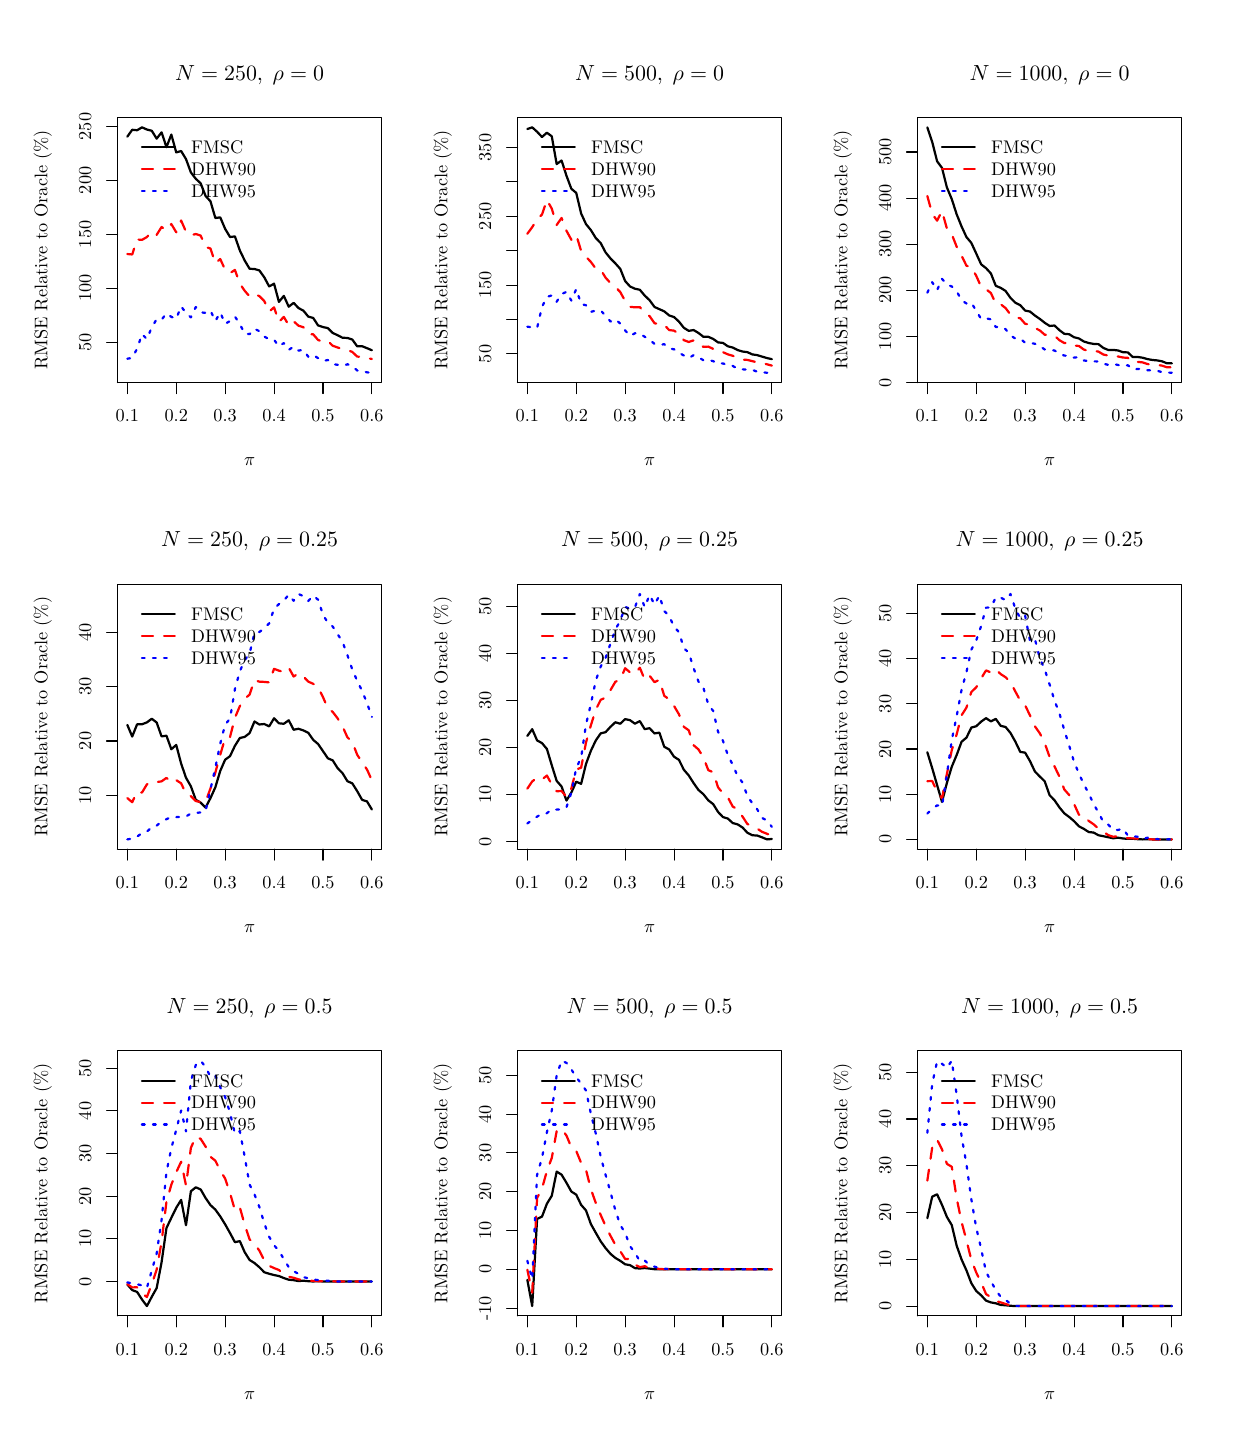
\begin{tikzpicture}[x=1pt,y=1pt]
\definecolor[named]{fillColor}{rgb}{1.00,1.00,1.00}
\path[use as bounding box,fill=fillColor,fill opacity=0.00] (0,0) rectangle (433.62,505.89);
\begin{scope}
\path[clip] ( 32.47,377.65) rectangle (127.91,473.42);
\definecolor[named]{drawColor}{rgb}{0.00,0.00,0.00}

\path[draw=drawColor,line width= 0.8pt,line join=round,line cap=round] ( 36.01,466.50) --
	( 37.77,468.99) --
	( 39.54,468.82) --
	( 41.31,469.87) --
	( 43.08,469.08) --
	( 44.84,468.64) --
	( 46.61,465.78) --
	( 48.38,468.06) --
	( 50.15,462.70) --
	( 51.91,467.27) --
	( 53.68,460.80) --
	( 55.45,461.32) --
	( 57.21,458.40) --
	( 58.98,453.57) --
	( 60.75,451.28) --
	( 62.52,449.63) --
	( 64.28,445.08) --
	( 66.05,443.15) --
	( 67.82,437.11) --
	( 69.59,437.33) --
	( 71.35,433.20) --
	( 73.12,430.23) --
	( 74.89,430.46) --
	( 76.66,425.40) --
	( 78.42,421.75) --
	( 80.19,418.76) --
	( 81.96,418.68) --
	( 83.72,418.17) --
	( 85.49,415.69) --
	( 87.26,412.38) --
	( 89.03,413.37) --
	( 90.79,406.80) --
	( 92.56,408.97) --
	( 94.33,405.06) --
	( 96.10,406.45) --
	( 97.86,404.57) --
	( 99.63,403.63) --
	(101.40,401.48) --
	(103.17,401.00) --
	(104.93,398.30) --
	(106.70,397.70) --
	(108.47,397.32) --
	(110.23,395.57) --
	(112.00,394.75) --
	(113.77,393.83) --
	(115.54,393.77) --
	(117.30,393.19) --
	(119.07,390.74) --
	(120.84,390.78) --
	(122.61,390.08) --
	(124.37,389.32);
\end{scope}
\begin{scope}
\path[clip] (  0.00,  0.00) rectangle (433.62,505.89);
\definecolor[named]{drawColor}{rgb}{0.00,0.00,0.00}

\path[draw=drawColor,line width= 0.4pt,line join=round,line cap=round] ( 36.01,377.65) -- (124.37,377.65);

\path[draw=drawColor,line width= 0.4pt,line join=round,line cap=round] ( 36.01,377.65) -- ( 36.01,373.69);

\path[draw=drawColor,line width= 0.4pt,line join=round,line cap=round] ( 53.68,377.65) -- ( 53.68,373.69);

\path[draw=drawColor,line width= 0.4pt,line join=round,line cap=round] ( 71.35,377.65) -- ( 71.35,373.69);

\path[draw=drawColor,line width= 0.4pt,line join=round,line cap=round] ( 89.03,377.65) -- ( 89.03,373.69);

\path[draw=drawColor,line width= 0.4pt,line join=round,line cap=round] (106.70,377.65) -- (106.70,373.69);

\path[draw=drawColor,line width= 0.4pt,line join=round,line cap=round] (124.37,377.65) -- (124.37,373.69);

\node[text=drawColor,anchor=base,inner sep=0pt, outer sep=0pt, scale=  0.66] at ( 36.01,363.40) {0.1};

\node[text=drawColor,anchor=base,inner sep=0pt, outer sep=0pt, scale=  0.66] at ( 53.68,363.40) {0.2};

\node[text=drawColor,anchor=base,inner sep=0pt, outer sep=0pt, scale=  0.66] at ( 71.35,363.40) {0.3};

\node[text=drawColor,anchor=base,inner sep=0pt, outer sep=0pt, scale=  0.66] at ( 89.03,363.40) {0.4};

\node[text=drawColor,anchor=base,inner sep=0pt, outer sep=0pt, scale=  0.66] at (106.70,363.40) {0.5};

\node[text=drawColor,anchor=base,inner sep=0pt, outer sep=0pt, scale=  0.66] at (124.37,363.40) {0.6};

\path[draw=drawColor,line width= 0.4pt,line join=round,line cap=round] ( 32.47,392.27) -- ( 32.47,470.18);

\path[draw=drawColor,line width= 0.4pt,line join=round,line cap=round] ( 32.47,392.27) -- ( 28.51,392.27);

\path[draw=drawColor,line width= 0.4pt,line join=round,line cap=round] ( 32.47,411.75) -- ( 28.51,411.75);

\path[draw=drawColor,line width= 0.4pt,line join=round,line cap=round] ( 32.47,431.22) -- ( 28.51,431.22);

\path[draw=drawColor,line width= 0.4pt,line join=round,line cap=round] ( 32.47,450.70) -- ( 28.51,450.70);

\path[draw=drawColor,line width= 0.4pt,line join=round,line cap=round] ( 32.47,470.18) -- ( 28.51,470.18);

\node[text=drawColor,rotate= 90.00,anchor=base,inner sep=0pt, outer sep=0pt, scale=  0.66] at ( 22.97,392.27) {50};

\node[text=drawColor,rotate= 90.00,anchor=base,inner sep=0pt, outer sep=0pt, scale=  0.66] at ( 22.97,411.75) {100};

\node[text=drawColor,rotate= 90.00,anchor=base,inner sep=0pt, outer sep=0pt, scale=  0.66] at ( 22.97,431.22) {150};

\node[text=drawColor,rotate= 90.00,anchor=base,inner sep=0pt, outer sep=0pt, scale=  0.66] at ( 22.97,450.70) {200};

\node[text=drawColor,rotate= 90.00,anchor=base,inner sep=0pt, outer sep=0pt, scale=  0.66] at ( 22.97,470.18) {250};

\path[draw=drawColor,line width= 0.4pt,line join=round,line cap=round] ( 32.47,377.65) --
	(127.91,377.65) --
	(127.91,473.42) --
	( 32.47,473.42) --
	( 32.47,377.65);
\end{scope}
\begin{scope}
\path[clip] (  0.00,337.26) rectangle (144.54,505.89);
\definecolor[named]{drawColor}{rgb}{0.00,0.00,0.00}

\node[text=drawColor,anchor=base,inner sep=0pt, outer sep=0pt, scale=  0.79] at ( 80.19,486.92) {\bfseries $N=250, \;\rho=0$};

\node[text=drawColor,anchor=base,inner sep=0pt, outer sep=0pt, scale=  0.66] at ( 80.19,347.56) {$\pi$};

\node[text=drawColor,rotate= 90.00,anchor=base,inner sep=0pt, outer sep=0pt, scale=  0.66] at (  7.13,425.53) {RMSE Relative to Oracle (\%)};
\end{scope}
\begin{scope}
\path[clip] ( 32.47,377.65) rectangle (127.91,473.42);
\definecolor[named]{drawColor}{rgb}{1.00,0.00,0.00}

\path[draw=drawColor,line width= 0.8pt,dash pattern=on 4pt off 4pt ,line join=round,line cap=round] ( 36.01,424.09) --
	( 37.77,423.93) --
	( 39.54,429.35) --
	( 41.31,429.20) --
	( 43.08,430.23) --
	( 44.84,432.19) --
	( 46.61,431.03) --
	( 48.38,433.85) --
	( 50.15,432.69) --
	( 51.91,434.93) --
	( 53.68,431.95) --
	( 55.45,436.20) --
	( 57.21,432.17) --
	( 58.98,430.86) --
	( 60.75,431.32) --
	( 62.52,430.75) --
	( 64.28,426.63) --
	( 66.05,426.09) --
	( 67.82,420.75) --
	( 69.59,422.28) --
	( 71.35,418.38) --
	( 73.12,417.19) --
	( 74.89,418.35) --
	( 76.66,413.39) --
	( 78.42,410.81) --
	( 80.19,408.76) --
	( 81.96,409.68) --
	( 83.72,408.87) --
	( 85.49,407.10) --
	( 87.26,403.28) --
	( 89.03,404.82) --
	( 90.79,399.52) --
	( 92.56,401.38) --
	( 94.33,398.33) --
	( 96.10,399.79) --
	( 97.86,398.20) --
	( 99.63,397.63) --
	(101.40,395.14) --
	(103.17,395.09) --
	(104.93,393.03) --
	(106.70,392.37) --
	(108.47,392.61) --
	(110.23,390.94) --
	(112.00,390.32) --
	(113.77,389.76) --
	(115.54,389.41) --
	(117.30,388.71) --
	(119.07,387.04) --
	(120.84,386.90) --
	(122.61,386.52) --
	(124.37,386.17);
\definecolor[named]{drawColor}{rgb}{0.00,0.00,1.00}

\path[draw=drawColor,line width= 0.8pt,dash pattern=on 1pt off 3pt ,line join=round,line cap=round] ( 36.01,386.26) --
	( 37.77,386.55) --
	( 39.54,389.89) --
	( 41.31,395.15) --
	( 43.08,393.36) --
	( 44.84,397.60) --
	( 46.61,400.55) --
	( 48.38,400.34) --
	( 50.15,402.66) --
	( 51.91,401.39) --
	( 53.68,400.69) --
	( 55.45,405.20) --
	( 57.21,402.74) --
	( 58.98,401.21) --
	( 60.75,404.93) --
	( 62.52,403.02) --
	( 64.28,402.82) --
	( 66.05,403.64) --
	( 67.82,399.88) --
	( 69.59,402.98) --
	( 71.35,398.87) --
	( 73.12,399.89) --
	( 74.89,401.49) --
	( 76.66,398.81) --
	( 78.42,395.31) --
	( 80.19,395.15) --
	( 81.96,397.07) --
	( 83.72,396.22) --
	( 85.49,394.29) --
	( 87.26,393.28) --
	( 89.03,393.10) --
	( 90.79,390.73) --
	( 92.56,391.93) --
	( 94.33,389.46) --
	( 96.10,390.62) --
	( 97.86,389.21) --
	( 99.63,389.44) --
	(101.40,386.97) --
	(103.17,387.66) --
	(104.93,386.46) --
	(106.70,385.45) --
	(108.47,385.79) --
	(110.23,384.32) --
	(112.00,384.06) --
	(113.77,383.68) --
	(115.54,384.25) --
	(117.30,383.63) --
	(119.07,382.00) --
	(120.84,381.80) --
	(122.61,381.34) --
	(124.37,381.20);
\definecolor[named]{drawColor}{rgb}{0.00,0.00,0.00}

\path[draw=drawColor,line width= 0.8pt,line join=round,line cap=round] ( 41.28,462.63) -- ( 53.16,462.63);
\definecolor[named]{drawColor}{rgb}{1.00,0.00,0.00}

\path[draw=drawColor,line width= 0.8pt,dash pattern=on 4pt off 4pt ,line join=round,line cap=round] ( 41.28,454.71) -- ( 53.16,454.71);
\definecolor[named]{drawColor}{rgb}{0.00,0.00,1.00}

\path[draw=drawColor,line width= 0.8pt,dash pattern=on 1pt off 3pt ,line join=round,line cap=round] ( 41.28,446.79) -- ( 53.16,446.79);
\definecolor[named]{drawColor}{rgb}{0.00,0.00,0.00}

\node[text=drawColor,anchor=base west,inner sep=0pt, outer sep=0pt, scale=  0.66] at ( 59.10,460.35) {FMSC};

\node[text=drawColor,anchor=base west,inner sep=0pt, outer sep=0pt, scale=  0.66] at ( 59.10,452.43) {DHW90};

\node[text=drawColor,anchor=base west,inner sep=0pt, outer sep=0pt, scale=  0.66] at ( 59.10,444.51) {DHW95};
\end{scope}
\begin{scope}
\path[clip] (177.01,377.65) rectangle (272.45,473.42);
\definecolor[named]{drawColor}{rgb}{0.00,0.00,0.00}

\path[draw=drawColor,line width= 0.8pt,line join=round,line cap=round] (180.55,469.26) --
	(182.31,469.87) --
	(184.08,468.27) --
	(185.85,466.38) --
	(187.62,467.93) --
	(189.38,466.64) --
	(191.15,456.59) --
	(192.92,457.89) --
	(194.69,452.39) --
	(196.45,447.68) --
	(198.22,446.19) --
	(199.99,438.74) --
	(201.75,434.90) --
	(203.52,432.73) --
	(205.29,429.86) --
	(207.06,428.05) --
	(208.82,424.69) --
	(210.59,422.49) --
	(212.36,420.71) --
	(214.13,418.72) --
	(215.89,414.33) --
	(217.66,412.37) --
	(219.43,411.55) --
	(221.20,411.18) --
	(222.96,409.08) --
	(224.73,407.39) --
	(226.50,404.97) --
	(228.26,404.17) --
	(230.03,403.37) --
	(231.80,401.90) --
	(233.57,401.31) --
	(235.33,399.68) --
	(237.10,397.44) --
	(238.87,396.33) --
	(240.64,396.62) --
	(242.40,395.57) --
	(244.17,394.18) --
	(245.94,394.18) --
	(247.71,393.41) --
	(249.47,392.16) --
	(251.24,391.97) --
	(253.01,390.75) --
	(254.77,390.31) --
	(256.54,389.39) --
	(258.31,388.86) --
	(260.08,388.63) --
	(261.84,387.82) --
	(263.61,387.56) --
	(265.38,387.02) --
	(267.15,386.50) --
	(268.91,386.10);
\end{scope}
\begin{scope}
\path[clip] (  0.00,  0.00) rectangle (433.62,505.89);
\definecolor[named]{drawColor}{rgb}{0.00,0.00,0.00}

\path[draw=drawColor,line width= 0.4pt,line join=round,line cap=round] (180.55,377.65) -- (268.91,377.65);

\path[draw=drawColor,line width= 0.4pt,line join=round,line cap=round] (180.55,377.65) -- (180.55,373.69);

\path[draw=drawColor,line width= 0.4pt,line join=round,line cap=round] (198.22,377.65) -- (198.22,373.69);

\path[draw=drawColor,line width= 0.4pt,line join=round,line cap=round] (215.89,377.65) -- (215.89,373.69);

\path[draw=drawColor,line width= 0.4pt,line join=round,line cap=round] (233.57,377.65) -- (233.57,373.69);

\path[draw=drawColor,line width= 0.4pt,line join=round,line cap=round] (251.24,377.65) -- (251.24,373.69);

\path[draw=drawColor,line width= 0.4pt,line join=round,line cap=round] (268.91,377.65) -- (268.91,373.69);

\node[text=drawColor,anchor=base,inner sep=0pt, outer sep=0pt, scale=  0.66] at (180.55,363.40) {0.1};

\node[text=drawColor,anchor=base,inner sep=0pt, outer sep=0pt, scale=  0.66] at (198.22,363.40) {0.2};

\node[text=drawColor,anchor=base,inner sep=0pt, outer sep=0pt, scale=  0.66] at (215.89,363.40) {0.3};

\node[text=drawColor,anchor=base,inner sep=0pt, outer sep=0pt, scale=  0.66] at (233.57,363.40) {0.4};

\node[text=drawColor,anchor=base,inner sep=0pt, outer sep=0pt, scale=  0.66] at (251.24,363.40) {0.5};

\node[text=drawColor,anchor=base,inner sep=0pt, outer sep=0pt, scale=  0.66] at (268.91,363.40) {0.6};

\path[draw=drawColor,line width= 0.4pt,line join=round,line cap=round] (177.01,388.00) -- (177.01,462.59);

\path[draw=drawColor,line width= 0.4pt,line join=round,line cap=round] (177.01,388.00) -- (173.05,388.00);

\path[draw=drawColor,line width= 0.4pt,line join=round,line cap=round] (177.01,400.43) -- (173.05,400.43);

\path[draw=drawColor,line width= 0.4pt,line join=round,line cap=round] (177.01,412.86) -- (173.05,412.86);

\path[draw=drawColor,line width= 0.4pt,line join=round,line cap=round] (177.01,425.29) -- (173.05,425.29);

\path[draw=drawColor,line width= 0.4pt,line join=round,line cap=round] (177.01,437.72) -- (173.05,437.72);

\path[draw=drawColor,line width= 0.4pt,line join=round,line cap=round] (177.01,450.15) -- (173.05,450.15);

\path[draw=drawColor,line width= 0.4pt,line join=round,line cap=round] (177.01,462.59) -- (173.05,462.59);

\node[text=drawColor,rotate= 90.00,anchor=base,inner sep=0pt, outer sep=0pt, scale=  0.66] at (167.51,388.00) {50};

\node[text=drawColor,rotate= 90.00,anchor=base,inner sep=0pt, outer sep=0pt, scale=  0.66] at (167.51,412.86) {150};

\node[text=drawColor,rotate= 90.00,anchor=base,inner sep=0pt, outer sep=0pt, scale=  0.66] at (167.51,437.72) {250};

\node[text=drawColor,rotate= 90.00,anchor=base,inner sep=0pt, outer sep=0pt, scale=  0.66] at (167.51,462.59) {350};

\path[draw=drawColor,line width= 0.4pt,line join=round,line cap=round] (177.01,377.65) --
	(272.45,377.65) --
	(272.45,473.42) --
	(177.01,473.42) --
	(177.01,377.65);
\end{scope}
\begin{scope}
\path[clip] (144.54,337.26) rectangle (289.08,505.89);
\definecolor[named]{drawColor}{rgb}{0.00,0.00,0.00}

\node[text=drawColor,anchor=base,inner sep=0pt, outer sep=0pt, scale=  0.79] at (224.73,486.92) {\bfseries $N=500, \;\rho=0$};

\node[text=drawColor,anchor=base,inner sep=0pt, outer sep=0pt, scale=  0.66] at (224.73,347.56) {$\pi$};

\node[text=drawColor,rotate= 90.00,anchor=base,inner sep=0pt, outer sep=0pt, scale=  0.66] at (151.67,425.53) {RMSE Relative to Oracle (\%)};
\end{scope}
\begin{scope}
\path[clip] (177.01,377.65) rectangle (272.45,473.42);
\definecolor[named]{drawColor}{rgb}{1.00,0.00,0.00}

\path[draw=drawColor,line width= 0.8pt,dash pattern=on 4pt off 4pt ,line join=round,line cap=round] (180.55,431.40) --
	(182.31,433.79) --
	(184.08,436.64) --
	(185.85,438.38) --
	(187.62,443.64) --
	(189.38,440.50) --
	(191.15,434.60) --
	(192.92,437.13) --
	(194.69,432.50) --
	(196.45,429.26) --
	(198.22,431.04) --
	(199.99,425.19) --
	(201.75,423.11) --
	(203.52,421.22) --
	(205.29,418.82) --
	(207.06,418.44) --
	(208.82,415.55) --
	(210.59,413.60) --
	(212.36,412.20) --
	(214.13,410.34) --
	(215.89,407.14) --
	(217.66,405.01) --
	(219.43,404.83) --
	(221.20,404.91) --
	(222.96,402.71) --
	(224.73,401.65) --
	(226.50,399.10) --
	(228.26,398.66) --
	(230.03,398.47) --
	(231.80,396.61) --
	(233.57,396.41) --
	(235.33,395.24) --
	(237.10,392.97) --
	(238.87,392.31) --
	(240.64,392.89) --
	(242.40,391.90) --
	(244.17,390.54) --
	(245.94,390.64) --
	(247.71,389.81) --
	(249.47,388.69) --
	(251.24,388.63) --
	(253.01,387.83) --
	(254.77,387.32) --
	(256.54,386.58) --
	(258.31,385.95) --
	(260.08,385.83) --
	(261.84,385.39) --
	(263.61,384.94) --
	(265.38,384.72) --
	(267.15,384.25) --
	(268.91,383.77);
\definecolor[named]{drawColor}{rgb}{0.00,0.00,1.00}

\path[draw=drawColor,line width= 0.8pt,dash pattern=on 1pt off 3pt ,line join=round,line cap=round] (180.55,397.83) --
	(182.31,397.61) --
	(184.08,397.41) --
	(185.85,405.02) --
	(187.62,408.59) --
	(189.38,409.15) --
	(191.15,406.87) --
	(192.92,409.65) --
	(194.69,410.41) --
	(196.45,407.29) --
	(198.22,411.43) --
	(199.99,406.05) --
	(201.75,405.56) --
	(203.52,403.20) --
	(205.29,403.66) --
	(207.06,403.67) --
	(208.82,401.83) --
	(210.59,399.70) --
	(212.36,400.54) --
	(214.13,398.95) --
	(215.89,396.50) --
	(217.66,394.49) --
	(219.43,395.46) --
	(221.20,395.36) --
	(222.96,394.20) --
	(224.73,393.04) --
	(226.50,391.64) --
	(228.26,391.18) --
	(230.03,391.52) --
	(231.80,390.01) --
	(233.57,389.65) --
	(235.33,388.38) --
	(237.10,387.44) --
	(238.87,386.52) --
	(240.64,387.55) --
	(242.40,386.84) --
	(244.17,385.68) --
	(245.94,385.82) --
	(247.71,385.39) --
	(249.47,384.45) --
	(251.24,384.57) --
	(253.01,383.88) --
	(254.77,383.65) --
	(256.54,382.65) --
	(258.31,382.43) --
	(260.08,382.29) --
	(261.84,382.25) --
	(263.61,381.55) --
	(265.38,381.35) --
	(267.15,381.20) --
	(268.91,381.20);
\definecolor[named]{drawColor}{rgb}{0.00,0.00,0.00}

\path[draw=drawColor,line width= 0.8pt,line join=round,line cap=round] (185.82,462.63) -- (197.70,462.63);
\definecolor[named]{drawColor}{rgb}{1.00,0.00,0.00}

\path[draw=drawColor,line width= 0.8pt,dash pattern=on 4pt off 4pt ,line join=round,line cap=round] (185.82,454.71) -- (197.70,454.71);
\definecolor[named]{drawColor}{rgb}{0.00,0.00,1.00}

\path[draw=drawColor,line width= 0.8pt,dash pattern=on 1pt off 3pt ,line join=round,line cap=round] (185.82,446.79) -- (197.70,446.79);
\definecolor[named]{drawColor}{rgb}{0.00,0.00,0.00}

\node[text=drawColor,anchor=base west,inner sep=0pt, outer sep=0pt, scale=  0.66] at (203.64,460.35) {FMSC};

\node[text=drawColor,anchor=base west,inner sep=0pt, outer sep=0pt, scale=  0.66] at (203.64,452.43) {DHW90};

\node[text=drawColor,anchor=base west,inner sep=0pt, outer sep=0pt, scale=  0.66] at (203.64,444.51) {DHW95};
\end{scope}
\begin{scope}
\path[clip] (321.55,377.65) rectangle (416.99,473.42);
\definecolor[named]{drawColor}{rgb}{0.00,0.00,0.00}

\path[draw=drawColor,line width= 0.8pt,line join=round,line cap=round] (325.09,469.87) --
	(326.85,464.60) --
	(328.62,457.60) --
	(330.39,455.22) --
	(332.16,448.15) --
	(333.92,443.94) --
	(335.69,438.44) --
	(337.46,434.05) --
	(339.23,430.21) --
	(340.99,428.11) --
	(342.76,424.28) --
	(344.53,420.37) --
	(346.29,419.00) --
	(348.06,417.07) --
	(349.83,412.59) --
	(351.60,411.87) --
	(353.36,410.75) --
	(355.13,408.24) --
	(356.90,406.48) --
	(358.67,405.60) --
	(360.43,403.66) --
	(362.20,403.30) --
	(363.97,401.85) --
	(365.74,400.64) --
	(367.50,399.26) --
	(369.27,398.10) --
	(371.04,398.26) --
	(372.80,396.60) --
	(374.57,395.26) --
	(376.34,395.11) --
	(378.11,394.02) --
	(379.87,393.58) --
	(381.64,392.48) --
	(383.41,391.94) --
	(385.18,391.61) --
	(386.94,391.52) --
	(388.71,390.14) --
	(390.48,389.42) --
	(392.25,389.45) --
	(394.01,389.24) --
	(395.78,388.61) --
	(397.55,388.54) --
	(399.31,386.88) --
	(401.08,386.89) --
	(402.85,386.63) --
	(404.62,386.13) --
	(406.38,385.81) --
	(408.15,385.65) --
	(409.92,385.32) --
	(411.69,384.60) --
	(413.45,384.60);
\end{scope}
\begin{scope}
\path[clip] (  0.00,  0.00) rectangle (433.62,505.89);
\definecolor[named]{drawColor}{rgb}{0.00,0.00,0.00}

\path[draw=drawColor,line width= 0.4pt,line join=round,line cap=round] (325.09,377.65) -- (413.45,377.65);

\path[draw=drawColor,line width= 0.4pt,line join=round,line cap=round] (325.09,377.65) -- (325.09,373.69);

\path[draw=drawColor,line width= 0.4pt,line join=round,line cap=round] (342.76,377.65) -- (342.76,373.69);

\path[draw=drawColor,line width= 0.4pt,line join=round,line cap=round] (360.43,377.65) -- (360.43,373.69);

\path[draw=drawColor,line width= 0.4pt,line join=round,line cap=round] (378.11,377.65) -- (378.11,373.69);

\path[draw=drawColor,line width= 0.4pt,line join=round,line cap=round] (395.78,377.65) -- (395.78,373.69);

\path[draw=drawColor,line width= 0.4pt,line join=round,line cap=round] (413.45,377.65) -- (413.45,373.69);

\node[text=drawColor,anchor=base,inner sep=0pt, outer sep=0pt, scale=  0.66] at (325.09,363.40) {0.1};

\node[text=drawColor,anchor=base,inner sep=0pt, outer sep=0pt, scale=  0.66] at (342.76,363.40) {0.2};

\node[text=drawColor,anchor=base,inner sep=0pt, outer sep=0pt, scale=  0.66] at (360.43,363.40) {0.3};

\node[text=drawColor,anchor=base,inner sep=0pt, outer sep=0pt, scale=  0.66] at (378.11,363.40) {0.4};

\node[text=drawColor,anchor=base,inner sep=0pt, outer sep=0pt, scale=  0.66] at (395.78,363.40) {0.5};

\node[text=drawColor,anchor=base,inner sep=0pt, outer sep=0pt, scale=  0.66] at (413.45,363.40) {0.6};

\path[draw=drawColor,line width= 0.4pt,line join=round,line cap=round] (321.55,377.68) -- (321.55,460.95);

\path[draw=drawColor,line width= 0.4pt,line join=round,line cap=round] (321.55,377.68) -- (317.59,377.68);

\path[draw=drawColor,line width= 0.4pt,line join=round,line cap=round] (321.55,394.34) -- (317.59,394.34);

\path[draw=drawColor,line width= 0.4pt,line join=round,line cap=round] (321.55,410.99) -- (317.59,410.99);

\path[draw=drawColor,line width= 0.4pt,line join=round,line cap=round] (321.55,427.64) -- (317.59,427.64);

\path[draw=drawColor,line width= 0.4pt,line join=round,line cap=round] (321.55,444.30) -- (317.59,444.30);

\path[draw=drawColor,line width= 0.4pt,line join=round,line cap=round] (321.55,460.95) -- (317.59,460.95);

\node[text=drawColor,rotate= 90.00,anchor=base,inner sep=0pt, outer sep=0pt, scale=  0.66] at (312.05,377.68) {0};

\node[text=drawColor,rotate= 90.00,anchor=base,inner sep=0pt, outer sep=0pt, scale=  0.66] at (312.05,394.34) {100};

\node[text=drawColor,rotate= 90.00,anchor=base,inner sep=0pt, outer sep=0pt, scale=  0.66] at (312.05,410.99) {200};

\node[text=drawColor,rotate= 90.00,anchor=base,inner sep=0pt, outer sep=0pt, scale=  0.66] at (312.05,427.64) {300};

\node[text=drawColor,rotate= 90.00,anchor=base,inner sep=0pt, outer sep=0pt, scale=  0.66] at (312.05,444.30) {400};

\node[text=drawColor,rotate= 90.00,anchor=base,inner sep=0pt, outer sep=0pt, scale=  0.66] at (312.05,460.95) {500};

\path[draw=drawColor,line width= 0.4pt,line join=round,line cap=round] (321.55,377.65) --
	(416.99,377.65) --
	(416.99,473.42) --
	(321.55,473.42) --
	(321.55,377.65);
\end{scope}
\begin{scope}
\path[clip] (289.08,337.26) rectangle (433.62,505.89);
\definecolor[named]{drawColor}{rgb}{0.00,0.00,0.00}

\node[text=drawColor,anchor=base,inner sep=0pt, outer sep=0pt, scale=  0.79] at (369.27,486.92) {\bfseries $N=1000, \;\rho=0$};

\node[text=drawColor,anchor=base,inner sep=0pt, outer sep=0pt, scale=  0.66] at (369.27,347.56) {$\pi$};

\node[text=drawColor,rotate= 90.00,anchor=base,inner sep=0pt, outer sep=0pt, scale=  0.66] at (296.21,425.53) {RMSE Relative to Oracle (\%)};
\end{scope}
\begin{scope}
\path[clip] (321.55,377.65) rectangle (416.99,473.42);
\definecolor[named]{drawColor}{rgb}{1.00,0.00,0.00}

\path[draw=drawColor,line width= 0.8pt,dash pattern=on 4pt off 4pt ,line join=round,line cap=round] (325.09,445.06) --
	(326.85,438.61) --
	(328.62,436.14) --
	(330.39,439.65) --
	(332.16,433.28) --
	(333.92,431.24) --
	(335.69,426.73) --
	(337.46,423.51) --
	(339.23,419.85) --
	(340.99,419.45) --
	(342.76,416.21) --
	(344.53,412.24) --
	(346.29,411.39) --
	(348.06,410.00) --
	(349.83,406.15) --
	(351.60,405.94) --
	(353.36,404.56) --
	(355.13,402.20) --
	(356.90,401.15) --
	(358.67,400.88) --
	(360.43,398.89) --
	(362.20,398.53) --
	(363.97,397.39) --
	(365.74,396.48) --
	(367.50,394.94) --
	(369.27,394.74) --
	(371.04,394.60) --
	(372.80,392.97) --
	(374.57,391.94) --
	(376.34,391.97) --
	(378.11,391.03) --
	(379.87,390.86) --
	(381.64,389.57) --
	(383.41,389.03) --
	(385.18,389.11) --
	(386.94,388.83) --
	(388.71,387.76) --
	(390.48,387.39) --
	(392.25,387.08) --
	(394.01,387.07) --
	(395.78,386.69) --
	(397.55,386.57) --
	(399.31,384.92) --
	(401.08,385.12) --
	(402.85,384.94) --
	(404.62,384.33) --
	(406.38,384.18) --
	(408.15,384.05) --
	(409.92,383.76) --
	(411.69,383.17) --
	(413.45,383.15);
\definecolor[named]{drawColor}{rgb}{0.00,0.00,1.00}

\path[draw=drawColor,line width= 0.8pt,dash pattern=on 1pt off 3pt ,line join=round,line cap=round] (325.09,410.11) --
	(326.85,413.91) --
	(328.62,411.02) --
	(330.39,415.12) --
	(332.16,413.04) --
	(333.92,412.37) --
	(335.69,410.63) --
	(337.46,407.36) --
	(339.23,406.23) --
	(340.99,406.55) --
	(342.76,403.54) --
	(344.53,400.66) --
	(346.29,400.87) --
	(348.06,400.48) --
	(349.83,397.72) --
	(351.60,397.84) --
	(353.36,396.93) --
	(355.13,394.72) --
	(356.90,393.53) --
	(358.67,393.49) --
	(360.43,392.04) --
	(362.20,392.01) --
	(363.97,391.65) --
	(365.74,390.78) --
	(367.50,389.61) --
	(369.27,389.44) --
	(371.04,389.24) --
	(372.80,388.08) --
	(374.57,387.40) --
	(376.34,387.29) --
	(378.11,386.66) --
	(379.87,386.86) --
	(381.64,385.65) --
	(383.41,385.35) --
	(385.18,385.30) --
	(386.94,385.29) --
	(388.71,384.46) --
	(390.48,384.04) --
	(392.25,384.37) --
	(394.01,384.00) --
	(395.78,383.54) --
	(397.55,383.91) --
	(399.31,382.43) --
	(401.08,382.54) --
	(402.85,382.58) --
	(404.62,382.12) --
	(406.38,381.99) --
	(408.15,381.89) --
	(409.92,381.41) --
	(411.69,381.27) --
	(413.45,381.20);
\definecolor[named]{drawColor}{rgb}{0.00,0.00,0.00}

\path[draw=drawColor,line width= 0.8pt,line join=round,line cap=round] (330.36,462.63) -- (342.24,462.63);
\definecolor[named]{drawColor}{rgb}{1.00,0.00,0.00}

\path[draw=drawColor,line width= 0.8pt,dash pattern=on 4pt off 4pt ,line join=round,line cap=round] (330.36,454.71) -- (342.24,454.71);
\definecolor[named]{drawColor}{rgb}{0.00,0.00,1.00}

\path[draw=drawColor,line width= 0.8pt,dash pattern=on 1pt off 3pt ,line join=round,line cap=round] (330.36,446.79) -- (342.24,446.79);
\definecolor[named]{drawColor}{rgb}{0.00,0.00,0.00}

\node[text=drawColor,anchor=base west,inner sep=0pt, outer sep=0pt, scale=  0.66] at (348.18,460.35) {FMSC};

\node[text=drawColor,anchor=base west,inner sep=0pt, outer sep=0pt, scale=  0.66] at (348.18,452.43) {DHW90};

\node[text=drawColor,anchor=base west,inner sep=0pt, outer sep=0pt, scale=  0.66] at (348.18,444.51) {DHW95};
\end{scope}
\begin{scope}
\path[clip] ( 32.47,209.02) rectangle (127.91,304.79);
\definecolor[named]{drawColor}{rgb}{0.00,0.00,0.00}

\path[draw=drawColor,line width= 0.8pt,line join=round,line cap=round] ( 36.01,253.94) --
	( 37.77,249.74) --
	( 39.54,254.14) --
	( 41.31,254.17) --
	( 43.08,254.85) --
	( 44.84,256.17) --
	( 46.61,254.81) --
	( 48.38,249.79) --
	( 50.15,250.04) --
	( 51.91,245.14) --
	( 53.68,246.71) --
	( 55.45,239.97) --
	( 57.21,234.85) --
	( 58.98,231.74) --
	( 60.75,226.87) --
	( 62.52,225.85) --
	( 64.28,224.06) --
	( 66.05,227.48) --
	( 67.82,231.42) --
	( 69.59,237.33) --
	( 71.35,241.37) --
	( 73.12,242.65) --
	( 74.89,246.39) --
	( 76.66,249.21) --
	( 78.42,249.61) --
	( 80.19,250.98) --
	( 81.96,255.18) --
	( 83.72,254.09) --
	( 85.49,254.26) --
	( 87.26,253.41) --
	( 89.03,256.35) --
	( 90.79,254.52) --
	( 92.56,254.35) --
	( 94.33,255.61) --
	( 96.10,252.19) --
	( 97.86,252.55) --
	( 99.63,251.94) --
	(101.40,251.09) --
	(103.17,248.54) --
	(104.93,247.05) --
	(106.70,244.48) --
	(108.47,241.87) --
	(110.23,241.12) --
	(112.00,238.31) --
	(113.77,236.50) --
	(115.54,233.59) --
	(117.30,232.83) --
	(119.07,230.01) --
	(120.84,226.87) --
	(122.61,226.30) --
	(124.37,223.38);
\end{scope}
\begin{scope}
\path[clip] (  0.00,  0.00) rectangle (433.62,505.89);
\definecolor[named]{drawColor}{rgb}{0.00,0.00,0.00}

\path[draw=drawColor,line width= 0.4pt,line join=round,line cap=round] ( 36.01,209.02) -- (124.37,209.02);

\path[draw=drawColor,line width= 0.4pt,line join=round,line cap=round] ( 36.01,209.02) -- ( 36.01,205.06);

\path[draw=drawColor,line width= 0.4pt,line join=round,line cap=round] ( 53.68,209.02) -- ( 53.68,205.06);

\path[draw=drawColor,line width= 0.4pt,line join=round,line cap=round] ( 71.35,209.02) -- ( 71.35,205.06);

\path[draw=drawColor,line width= 0.4pt,line join=round,line cap=round] ( 89.03,209.02) -- ( 89.03,205.06);

\path[draw=drawColor,line width= 0.4pt,line join=round,line cap=round] (106.70,209.02) -- (106.70,205.06);

\path[draw=drawColor,line width= 0.4pt,line join=round,line cap=round] (124.37,209.02) -- (124.37,205.06);

\node[text=drawColor,anchor=base,inner sep=0pt, outer sep=0pt, scale=  0.66] at ( 36.01,194.77) {0.1};

\node[text=drawColor,anchor=base,inner sep=0pt, outer sep=0pt, scale=  0.66] at ( 53.68,194.77) {0.2};

\node[text=drawColor,anchor=base,inner sep=0pt, outer sep=0pt, scale=  0.66] at ( 71.35,194.77) {0.3};

\node[text=drawColor,anchor=base,inner sep=0pt, outer sep=0pt, scale=  0.66] at ( 89.03,194.77) {0.4};

\node[text=drawColor,anchor=base,inner sep=0pt, outer sep=0pt, scale=  0.66] at (106.70,194.77) {0.5};

\node[text=drawColor,anchor=base,inner sep=0pt, outer sep=0pt, scale=  0.66] at (124.37,194.77) {0.6};

\path[draw=drawColor,line width= 0.4pt,line join=round,line cap=round] ( 32.47,228.53) -- ( 32.47,287.37);

\path[draw=drawColor,line width= 0.4pt,line join=round,line cap=round] ( 32.47,228.53) -- ( 28.51,228.53);

\path[draw=drawColor,line width= 0.4pt,line join=round,line cap=round] ( 32.47,248.14) -- ( 28.51,248.14);

\path[draw=drawColor,line width= 0.4pt,line join=round,line cap=round] ( 32.47,267.75) -- ( 28.51,267.75);

\path[draw=drawColor,line width= 0.4pt,line join=round,line cap=round] ( 32.47,287.37) -- ( 28.51,287.37);

\node[text=drawColor,rotate= 90.00,anchor=base,inner sep=0pt, outer sep=0pt, scale=  0.66] at ( 22.97,228.53) {10};

\node[text=drawColor,rotate= 90.00,anchor=base,inner sep=0pt, outer sep=0pt, scale=  0.66] at ( 22.97,248.14) {20};

\node[text=drawColor,rotate= 90.00,anchor=base,inner sep=0pt, outer sep=0pt, scale=  0.66] at ( 22.97,267.75) {30};

\node[text=drawColor,rotate= 90.00,anchor=base,inner sep=0pt, outer sep=0pt, scale=  0.66] at ( 22.97,287.37) {40};

\path[draw=drawColor,line width= 0.4pt,line join=round,line cap=round] ( 32.47,209.02) --
	(127.91,209.02) --
	(127.91,304.79) --
	( 32.47,304.79) --
	( 32.47,209.02);
\end{scope}
\begin{scope}
\path[clip] (  0.00,168.63) rectangle (144.54,337.26);
\definecolor[named]{drawColor}{rgb}{0.00,0.00,0.00}

\node[text=drawColor,anchor=base,inner sep=0pt, outer sep=0pt, scale=  0.79] at ( 80.19,318.29) {\bfseries $N=250, \;\rho=0.25$};

\node[text=drawColor,anchor=base,inner sep=0pt, outer sep=0pt, scale=  0.66] at ( 80.19,178.93) {$\pi$};

\node[text=drawColor,rotate= 90.00,anchor=base,inner sep=0pt, outer sep=0pt, scale=  0.66] at (  7.13,256.90) {RMSE Relative to Oracle (\%)};
\end{scope}
\begin{scope}
\path[clip] ( 32.47,209.02) rectangle (127.91,304.79);
\definecolor[named]{drawColor}{rgb}{1.00,0.00,0.00}

\path[draw=drawColor,line width= 0.8pt,dash pattern=on 4pt off 4pt ,line join=round,line cap=round] ( 36.01,227.50) --
	( 37.77,226.01) --
	( 39.54,229.81) --
	( 41.31,229.49) --
	( 43.08,232.45) --
	( 44.84,233.40) --
	( 46.61,233.27) --
	( 48.38,233.55) --
	( 50.15,234.80) --
	( 51.91,233.14) --
	( 53.68,233.98) --
	( 55.45,232.84) --
	( 57.21,229.09) --
	( 58.98,228.18) --
	( 60.75,226.42) --
	( 62.52,226.08) --
	( 64.28,226.18) --
	( 66.05,230.98) --
	( 67.82,236.75) --
	( 69.59,243.16) --
	( 71.35,249.15) --
	( 73.12,249.58) --
	( 74.89,256.52) --
	( 76.66,260.72) --
	( 78.42,263.37) --
	( 80.19,264.89) --
	( 81.96,270.14) --
	( 83.72,269.57) --
	( 85.49,269.48) --
	( 87.26,269.30) --
	( 89.03,274.22) --
	( 90.79,273.53) --
	( 92.56,273.15) --
	( 94.33,274.62) --
	( 96.10,271.43) --
	( 97.86,272.56) --
	( 99.63,271.43) --
	(101.40,269.58) --
	(103.17,268.79) --
	(104.93,267.55) --
	(106.70,264.01) --
	(108.47,259.91) --
	(110.23,258.63) --
	(112.00,256.30) --
	(113.77,253.39) --
	(115.54,249.45) --
	(117.30,247.76) --
	(119.07,243.15) --
	(120.84,240.46) --
	(122.61,237.83) --
	(124.37,233.95);
\definecolor[named]{drawColor}{rgb}{0.00,0.00,1.00}

\path[draw=drawColor,line width= 0.8pt,dash pattern=on 1pt off 3pt ,line join=round,line cap=round] ( 36.01,212.57) --
	( 37.77,212.86) --
	( 39.54,213.58) --
	( 41.31,214.84) --
	( 43.08,215.35) --
	( 44.84,217.01) --
	( 46.61,217.55) --
	( 48.38,219.02) --
	( 50.15,219.87) --
	( 51.91,220.72) --
	( 53.68,220.63) --
	( 55.45,220.66) --
	( 57.21,220.86) --
	( 58.98,221.93) --
	( 60.75,222.12) --
	( 62.52,222.33) --
	( 64.28,222.80) --
	( 66.05,230.65) --
	( 67.82,238.50) --
	( 69.59,247.15) --
	( 71.35,254.09) --
	( 73.12,256.16) --
	( 74.89,266.90) --
	( 76.66,273.28) --
	( 78.42,277.37) --
	( 80.19,279.72) --
	( 81.96,287.19) --
	( 83.72,287.53) --
	( 85.49,288.79) --
	( 87.26,290.65) --
	( 89.03,295.94) --
	( 90.79,297.60) --
	( 92.56,298.87) --
	( 94.33,301.01) --
	( 96.10,298.81) --
	( 97.86,301.24) --
	( 99.63,300.46) --
	(101.40,298.74) --
	(103.17,300.64) --
	(104.93,299.18) --
	(106.70,293.79) --
	(108.47,290.80) --
	(110.23,289.48) --
	(112.00,286.73) --
	(113.77,283.94) --
	(115.54,279.14) --
	(117.30,273.94) --
	(119.07,269.89) --
	(120.84,266.20) --
	(122.61,261.87) --
	(124.37,256.83);
\definecolor[named]{drawColor}{rgb}{0.00,0.00,0.00}

\path[draw=drawColor,line width= 0.8pt,line join=round,line cap=round] ( 41.28,294.00) -- ( 53.16,294.00);
\definecolor[named]{drawColor}{rgb}{1.00,0.00,0.00}

\path[draw=drawColor,line width= 0.8pt,dash pattern=on 4pt off 4pt ,line join=round,line cap=round] ( 41.28,286.08) -- ( 53.16,286.08);
\definecolor[named]{drawColor}{rgb}{0.00,0.00,1.00}

\path[draw=drawColor,line width= 0.8pt,dash pattern=on 1pt off 3pt ,line join=round,line cap=round] ( 41.28,278.16) -- ( 53.16,278.16);
\definecolor[named]{drawColor}{rgb}{0.00,0.00,0.00}

\node[text=drawColor,anchor=base west,inner sep=0pt, outer sep=0pt, scale=  0.66] at ( 59.10,291.72) {FMSC};

\node[text=drawColor,anchor=base west,inner sep=0pt, outer sep=0pt, scale=  0.66] at ( 59.10,283.80) {DHW90};

\node[text=drawColor,anchor=base west,inner sep=0pt, outer sep=0pt, scale=  0.66] at ( 59.10,275.88) {DHW95};
\end{scope}
\begin{scope}
\path[clip] (177.01,209.02) rectangle (272.45,304.79);
\definecolor[named]{drawColor}{rgb}{0.00,0.00,0.00}

\path[draw=drawColor,line width= 0.8pt,line join=round,line cap=round] (180.55,249.96) --
	(182.31,252.39) --
	(184.08,248.34) --
	(185.85,247.36) --
	(187.62,245.25) --
	(189.38,239.36) --
	(191.15,233.71) --
	(192.92,231.69) --
	(194.69,226.60) --
	(196.45,229.48) --
	(198.22,233.42) --
	(199.99,232.65) --
	(201.75,239.84) --
	(203.52,244.61) --
	(205.29,248.33) --
	(207.06,250.89) --
	(208.82,251.32) --
	(210.59,253.25) --
	(212.36,254.90) --
	(214.13,254.36) --
	(215.89,256.04) --
	(217.66,255.65) --
	(219.43,254.38) --
	(221.20,255.32) --
	(222.96,252.40) --
	(224.73,252.75) --
	(226.50,250.85) --
	(228.26,251.15) --
	(230.03,246.04) --
	(231.80,245.07) --
	(233.57,242.44) --
	(235.33,241.32) --
	(237.10,237.75) --
	(238.87,235.68) --
	(240.64,232.91) --
	(242.40,230.42) --
	(244.17,228.90) --
	(245.94,226.68) --
	(247.71,225.31) --
	(249.47,222.48) --
	(251.24,220.64) --
	(253.01,220.09) --
	(254.77,218.48) --
	(256.54,218.00) --
	(258.31,216.87) --
	(260.08,214.96) --
	(261.84,214.07) --
	(263.61,213.96) --
	(265.38,213.31) --
	(267.15,212.57) --
	(268.91,212.72);
\end{scope}
\begin{scope}
\path[clip] (  0.00,  0.00) rectangle (433.62,505.89);
\definecolor[named]{drawColor}{rgb}{0.00,0.00,0.00}

\path[draw=drawColor,line width= 0.4pt,line join=round,line cap=round] (180.55,209.02) -- (268.91,209.02);

\path[draw=drawColor,line width= 0.4pt,line join=round,line cap=round] (180.55,209.02) -- (180.55,205.06);

\path[draw=drawColor,line width= 0.4pt,line join=round,line cap=round] (198.22,209.02) -- (198.22,205.06);

\path[draw=drawColor,line width= 0.4pt,line join=round,line cap=round] (215.89,209.02) -- (215.89,205.06);

\path[draw=drawColor,line width= 0.4pt,line join=round,line cap=round] (233.57,209.02) -- (233.57,205.06);

\path[draw=drawColor,line width= 0.4pt,line join=round,line cap=round] (251.24,209.02) -- (251.24,205.06);

\path[draw=drawColor,line width= 0.4pt,line join=round,line cap=round] (268.91,209.02) -- (268.91,205.06);

\node[text=drawColor,anchor=base,inner sep=0pt, outer sep=0pt, scale=  0.66] at (180.55,194.77) {0.1};

\node[text=drawColor,anchor=base,inner sep=0pt, outer sep=0pt, scale=  0.66] at (198.22,194.77) {0.2};

\node[text=drawColor,anchor=base,inner sep=0pt, outer sep=0pt, scale=  0.66] at (215.89,194.77) {0.3};

\node[text=drawColor,anchor=base,inner sep=0pt, outer sep=0pt, scale=  0.66] at (233.57,194.77) {0.4};

\node[text=drawColor,anchor=base,inner sep=0pt, outer sep=0pt, scale=  0.66] at (251.24,194.77) {0.5};

\node[text=drawColor,anchor=base,inner sep=0pt, outer sep=0pt, scale=  0.66] at (268.91,194.77) {0.6};

\path[draw=drawColor,line width= 0.4pt,line join=round,line cap=round] (177.01,211.83) -- (177.01,296.78);

\path[draw=drawColor,line width= 0.4pt,line join=round,line cap=round] (177.01,211.83) -- (173.05,211.83);

\path[draw=drawColor,line width= 0.4pt,line join=round,line cap=round] (177.01,228.82) -- (173.05,228.82);

\path[draw=drawColor,line width= 0.4pt,line join=round,line cap=round] (177.01,245.81) -- (173.05,245.81);

\path[draw=drawColor,line width= 0.4pt,line join=round,line cap=round] (177.01,262.80) -- (173.05,262.80);

\path[draw=drawColor,line width= 0.4pt,line join=round,line cap=round] (177.01,279.79) -- (173.05,279.79);

\path[draw=drawColor,line width= 0.4pt,line join=round,line cap=round] (177.01,296.78) -- (173.05,296.78);

\node[text=drawColor,rotate= 90.00,anchor=base,inner sep=0pt, outer sep=0pt, scale=  0.66] at (167.51,211.83) {0};

\node[text=drawColor,rotate= 90.00,anchor=base,inner sep=0pt, outer sep=0pt, scale=  0.66] at (167.51,228.82) {10};

\node[text=drawColor,rotate= 90.00,anchor=base,inner sep=0pt, outer sep=0pt, scale=  0.66] at (167.51,245.81) {20};

\node[text=drawColor,rotate= 90.00,anchor=base,inner sep=0pt, outer sep=0pt, scale=  0.66] at (167.51,262.80) {30};

\node[text=drawColor,rotate= 90.00,anchor=base,inner sep=0pt, outer sep=0pt, scale=  0.66] at (167.51,279.79) {40};

\node[text=drawColor,rotate= 90.00,anchor=base,inner sep=0pt, outer sep=0pt, scale=  0.66] at (167.51,296.78) {50};

\path[draw=drawColor,line width= 0.4pt,line join=round,line cap=round] (177.01,209.02) --
	(272.45,209.02) --
	(272.45,304.79) --
	(177.01,304.79) --
	(177.01,209.02);
\end{scope}
\begin{scope}
\path[clip] (144.54,168.63) rectangle (289.08,337.26);
\definecolor[named]{drawColor}{rgb}{0.00,0.00,0.00}

\node[text=drawColor,anchor=base,inner sep=0pt, outer sep=0pt, scale=  0.79] at (224.73,318.29) {\bfseries $N=500, \;\rho=0.25$};

\node[text=drawColor,anchor=base,inner sep=0pt, outer sep=0pt, scale=  0.66] at (224.73,178.93) {$\pi$};

\node[text=drawColor,rotate= 90.00,anchor=base,inner sep=0pt, outer sep=0pt, scale=  0.66] at (151.67,256.90) {RMSE Relative to Oracle (\%)};
\end{scope}
\begin{scope}
\path[clip] (177.01,209.02) rectangle (272.45,304.79);
\definecolor[named]{drawColor}{rgb}{1.00,0.00,0.00}

\path[draw=drawColor,line width= 0.8pt,dash pattern=on 4pt off 4pt ,line join=round,line cap=round] (180.55,230.92) --
	(182.31,233.51) --
	(184.08,234.88) --
	(185.85,234.22) --
	(187.62,235.64) --
	(189.38,232.42) --
	(191.15,229.98) --
	(192.92,230.04) --
	(194.69,227.95) --
	(196.45,230.97) --
	(198.22,237.83) --
	(199.99,238.47) --
	(201.75,247.58) --
	(203.52,253.83) --
	(205.29,259.45) --
	(207.06,262.99) --
	(208.82,263.83) --
	(210.59,266.49) --
	(212.36,269.53) --
	(214.13,270.30) --
	(215.89,274.42) --
	(217.66,272.92) --
	(219.43,272.42) --
	(221.20,274.61) --
	(222.96,270.30) --
	(224.73,271.71) --
	(226.50,269.39) --
	(228.26,270.24) --
	(230.03,264.46) --
	(231.80,263.17) --
	(233.57,260.78) --
	(235.33,257.79) --
	(237.10,253.26) --
	(238.87,252.00) --
	(240.64,246.59) --
	(242.40,245.07) --
	(244.17,242.18) --
	(245.94,237.60) --
	(247.71,236.83) --
	(249.47,231.39) --
	(251.24,229.18) --
	(253.01,227.75) --
	(254.77,224.44) --
	(256.54,223.42) --
	(258.31,220.79) --
	(260.08,218.12) --
	(261.84,217.36) --
	(263.61,216.46) --
	(265.38,215.30) --
	(267.15,214.60) --
	(268.91,213.84);
\definecolor[named]{drawColor}{rgb}{0.00,0.00,1.00}

\path[draw=drawColor,line width= 0.8pt,dash pattern=on 1pt off 3pt ,line join=round,line cap=round] (180.55,218.33) --
	(182.31,219.59) --
	(184.08,220.79) --
	(185.85,221.89) --
	(187.62,222.04) --
	(189.38,223.40) --
	(191.15,223.33) --
	(192.92,223.41) --
	(194.69,224.16) --
	(196.45,229.53) --
	(198.22,238.32) --
	(199.99,242.13) --
	(201.75,254.10) --
	(203.52,261.53) --
	(205.29,269.99) --
	(207.06,275.02) --
	(208.82,278.17) --
	(210.59,283.30) --
	(212.36,288.37) --
	(214.13,291.62) --
	(215.89,296.57) --
	(217.66,295.94) --
	(219.43,296.43) --
	(221.20,301.24) --
	(222.96,296.49) --
	(224.73,300.91) --
	(226.50,297.43) --
	(228.26,300.67) --
	(230.03,295.07) --
	(231.80,293.32) --
	(233.57,289.35) --
	(235.33,287.51) --
	(237.10,281.64) --
	(238.87,280.08) --
	(240.64,274.46) --
	(242.40,269.58) --
	(244.17,267.35) --
	(245.94,261.35) --
	(247.71,258.97) --
	(249.47,251.46) --
	(251.24,248.20) --
	(253.01,243.04) --
	(254.77,239.51) --
	(256.54,235.41) --
	(258.31,233.11) --
	(260.08,228.21) --
	(261.84,225.63) --
	(263.61,223.45) --
	(265.38,220.33) --
	(267.15,219.38) --
	(268.91,217.11);
\definecolor[named]{drawColor}{rgb}{0.00,0.00,0.00}

\path[draw=drawColor,line width= 0.8pt,line join=round,line cap=round] (185.82,294.00) -- (197.70,294.00);
\definecolor[named]{drawColor}{rgb}{1.00,0.00,0.00}

\path[draw=drawColor,line width= 0.8pt,dash pattern=on 4pt off 4pt ,line join=round,line cap=round] (185.82,286.08) -- (197.70,286.08);
\definecolor[named]{drawColor}{rgb}{0.00,0.00,1.00}

\path[draw=drawColor,line width= 0.8pt,dash pattern=on 1pt off 3pt ,line join=round,line cap=round] (185.82,278.16) -- (197.70,278.16);
\definecolor[named]{drawColor}{rgb}{0.00,0.00,0.00}

\node[text=drawColor,anchor=base west,inner sep=0pt, outer sep=0pt, scale=  0.66] at (203.64,291.72) {FMSC};

\node[text=drawColor,anchor=base west,inner sep=0pt, outer sep=0pt, scale=  0.66] at (203.64,283.80) {DHW90};

\node[text=drawColor,anchor=base west,inner sep=0pt, outer sep=0pt, scale=  0.66] at (203.64,275.88) {DHW95};
\end{scope}
\begin{scope}
\path[clip] (321.55,209.02) rectangle (416.99,304.79);
\definecolor[named]{drawColor}{rgb}{0.00,0.00,0.00}

\path[draw=drawColor,line width= 0.8pt,line join=round,line cap=round] (325.09,244.06) --
	(326.85,238.31) --
	(328.62,232.19) --
	(330.39,226.10) --
	(332.16,232.99) --
	(333.92,238.83) --
	(335.69,243.07) --
	(337.46,247.85) --
	(339.23,249.34) --
	(340.99,252.98) --
	(342.76,253.46) --
	(344.53,255.12) --
	(346.29,256.38) --
	(348.06,255.23) --
	(349.83,256.10) --
	(351.60,253.60) --
	(353.36,253.19) --
	(355.13,251.04) --
	(356.90,247.88) --
	(358.67,244.19) --
	(360.43,243.91) --
	(362.20,240.83) --
	(363.97,237.08) --
	(365.74,235.28) --
	(367.50,233.57) --
	(369.27,228.54) --
	(371.04,226.72) --
	(372.80,224.15) --
	(374.57,222.00) --
	(376.34,220.68) --
	(378.11,219.16) --
	(379.87,217.30) --
	(381.64,216.37) --
	(383.41,215.23) --
	(385.18,215.04) --
	(386.94,214.06) --
	(388.71,213.72) --
	(390.48,213.34) --
	(392.25,212.98) --
	(394.01,213.19) --
	(395.78,212.90) --
	(397.55,212.76) --
	(399.31,212.80) --
	(401.08,212.65) --
	(402.85,212.57) --
	(404.62,212.64) --
	(406.38,212.57) --
	(408.15,212.57) --
	(409.92,212.57) --
	(411.69,212.57) --
	(413.45,212.57);
\end{scope}
\begin{scope}
\path[clip] (  0.00,  0.00) rectangle (433.62,505.89);
\definecolor[named]{drawColor}{rgb}{0.00,0.00,0.00}

\path[draw=drawColor,line width= 0.4pt,line join=round,line cap=round] (325.09,209.02) -- (413.45,209.02);

\path[draw=drawColor,line width= 0.4pt,line join=round,line cap=round] (325.09,209.02) -- (325.09,205.06);

\path[draw=drawColor,line width= 0.4pt,line join=round,line cap=round] (342.76,209.02) -- (342.76,205.06);

\path[draw=drawColor,line width= 0.4pt,line join=round,line cap=round] (360.43,209.02) -- (360.43,205.06);

\path[draw=drawColor,line width= 0.4pt,line join=round,line cap=round] (378.11,209.02) -- (378.11,205.06);

\path[draw=drawColor,line width= 0.4pt,line join=round,line cap=round] (395.78,209.02) -- (395.78,205.06);

\path[draw=drawColor,line width= 0.4pt,line join=round,line cap=round] (413.45,209.02) -- (413.45,205.06);

\node[text=drawColor,anchor=base,inner sep=0pt, outer sep=0pt, scale=  0.66] at (325.09,194.77) {0.1};

\node[text=drawColor,anchor=base,inner sep=0pt, outer sep=0pt, scale=  0.66] at (342.76,194.77) {0.2};

\node[text=drawColor,anchor=base,inner sep=0pt, outer sep=0pt, scale=  0.66] at (360.43,194.77) {0.3};

\node[text=drawColor,anchor=base,inner sep=0pt, outer sep=0pt, scale=  0.66] at (378.11,194.77) {0.4};

\node[text=drawColor,anchor=base,inner sep=0pt, outer sep=0pt, scale=  0.66] at (395.78,194.77) {0.5};

\node[text=drawColor,anchor=base,inner sep=0pt, outer sep=0pt, scale=  0.66] at (413.45,194.77) {0.6};

\path[draw=drawColor,line width= 0.4pt,line join=round,line cap=round] (321.55,212.57) -- (321.55,294.19);

\path[draw=drawColor,line width= 0.4pt,line join=round,line cap=round] (321.55,212.57) -- (317.59,212.57);

\path[draw=drawColor,line width= 0.4pt,line join=round,line cap=round] (321.55,228.89) -- (317.59,228.89);

\path[draw=drawColor,line width= 0.4pt,line join=round,line cap=round] (321.55,245.22) -- (317.59,245.22);

\path[draw=drawColor,line width= 0.4pt,line join=round,line cap=round] (321.55,261.54) -- (317.59,261.54);

\path[draw=drawColor,line width= 0.4pt,line join=round,line cap=round] (321.55,277.87) -- (317.59,277.87);

\path[draw=drawColor,line width= 0.4pt,line join=round,line cap=round] (321.55,294.19) -- (317.59,294.19);

\node[text=drawColor,rotate= 90.00,anchor=base,inner sep=0pt, outer sep=0pt, scale=  0.66] at (312.05,212.57) {0};

\node[text=drawColor,rotate= 90.00,anchor=base,inner sep=0pt, outer sep=0pt, scale=  0.66] at (312.05,228.89) {10};

\node[text=drawColor,rotate= 90.00,anchor=base,inner sep=0pt, outer sep=0pt, scale=  0.66] at (312.05,245.22) {20};

\node[text=drawColor,rotate= 90.00,anchor=base,inner sep=0pt, outer sep=0pt, scale=  0.66] at (312.05,261.54) {30};

\node[text=drawColor,rotate= 90.00,anchor=base,inner sep=0pt, outer sep=0pt, scale=  0.66] at (312.05,277.87) {40};

\node[text=drawColor,rotate= 90.00,anchor=base,inner sep=0pt, outer sep=0pt, scale=  0.66] at (312.05,294.19) {50};

\path[draw=drawColor,line width= 0.4pt,line join=round,line cap=round] (321.55,209.02) --
	(416.99,209.02) --
	(416.99,304.79) --
	(321.55,304.79) --
	(321.55,209.02);
\end{scope}
\begin{scope}
\path[clip] (289.08,168.63) rectangle (433.62,337.26);
\definecolor[named]{drawColor}{rgb}{0.00,0.00,0.00}

\node[text=drawColor,anchor=base,inner sep=0pt, outer sep=0pt, scale=  0.79] at (369.27,318.29) {\bfseries $N=1000, \;\rho=0.25$};

\node[text=drawColor,anchor=base,inner sep=0pt, outer sep=0pt, scale=  0.66] at (369.27,178.93) {$\pi$};

\node[text=drawColor,rotate= 90.00,anchor=base,inner sep=0pt, outer sep=0pt, scale=  0.66] at (296.21,256.90) {RMSE Relative to Oracle (\%)};
\end{scope}
\begin{scope}
\path[clip] (321.55,209.02) rectangle (416.99,304.79);
\definecolor[named]{drawColor}{rgb}{1.00,0.00,0.00}

\path[draw=drawColor,line width= 0.8pt,dash pattern=on 4pt off 4pt ,line join=round,line cap=round] (325.09,233.61) --
	(326.85,233.66) --
	(328.62,229.86) --
	(330.39,227.40) --
	(332.16,236.26) --
	(333.92,244.84) --
	(335.69,250.55) --
	(337.46,257.41) --
	(339.23,260.21) --
	(340.99,265.83) --
	(342.76,267.54) --
	(344.53,270.72) --
	(346.29,273.64) --
	(348.06,272.89) --
	(349.83,273.98) --
	(351.60,272.30) --
	(353.36,271.17) --
	(355.13,269.40) --
	(356.90,265.99) --
	(358.67,262.73) --
	(360.43,261.01) --
	(362.20,257.34) --
	(363.97,253.42) --
	(365.74,250.89) --
	(367.50,247.36) --
	(369.27,242.36) --
	(371.04,238.96) --
	(372.80,235.28) --
	(374.57,230.63) --
	(376.34,228.61) --
	(378.11,225.37) --
	(379.87,221.48) --
	(381.64,221.23) --
	(383.41,219.24) --
	(385.18,218.03) --
	(386.94,216.42) --
	(388.71,215.32) --
	(390.48,214.10) --
	(392.25,213.53) --
	(394.01,213.74) --
	(395.78,213.60) --
	(397.55,212.96) --
	(399.31,212.94) --
	(401.08,212.84) --
	(402.85,212.57) --
	(404.62,212.71) --
	(406.38,212.57) --
	(408.15,212.57) --
	(409.92,212.57) --
	(411.69,212.57) --
	(413.45,212.57);
\definecolor[named]{drawColor}{rgb}{0.00,0.00,1.00}

\path[draw=drawColor,line width= 0.8pt,dash pattern=on 1pt off 3pt ,line join=round,line cap=round] (325.09,221.93) --
	(326.85,223.54) --
	(328.62,224.87) --
	(330.39,224.58) --
	(332.16,235.95) --
	(333.92,248.50) --
	(335.69,257.10) --
	(337.46,266.65) --
	(339.23,273.04) --
	(340.99,281.14) --
	(342.76,284.47) --
	(344.53,289.68) --
	(346.29,296.31) --
	(348.06,296.37) --
	(349.83,299.99) --
	(351.60,299.92) --
	(353.36,299.03) --
	(355.13,301.24) --
	(356.90,295.92) --
	(358.67,292.41) --
	(360.43,293.39) --
	(362.20,284.20) --
	(363.97,284.89) --
	(365.74,278.05) --
	(367.50,273.98) --
	(369.27,268.57) --
	(371.04,262.73) --
	(372.80,258.18) --
	(374.57,252.12) --
	(376.34,246.46) --
	(378.11,240.61) --
	(379.87,236.35) --
	(381.64,232.46) --
	(383.41,229.15) --
	(385.18,225.31) --
	(386.94,222.27) --
	(388.71,218.80) --
	(390.48,217.88) --
	(392.25,216.03) --
	(394.01,215.98) --
	(395.78,216.50) --
	(397.55,213.94) --
	(399.31,213.68) --
	(401.08,213.54) --
	(402.85,212.65) --
	(404.62,213.21) --
	(406.38,212.57) --
	(408.15,212.69) --
	(409.92,212.57) --
	(411.69,212.57) --
	(413.45,212.67);
\definecolor[named]{drawColor}{rgb}{0.00,0.00,0.00}

\path[draw=drawColor,line width= 0.8pt,line join=round,line cap=round] (330.36,294.00) -- (342.24,294.00);
\definecolor[named]{drawColor}{rgb}{1.00,0.00,0.00}

\path[draw=drawColor,line width= 0.8pt,dash pattern=on 4pt off 4pt ,line join=round,line cap=round] (330.36,286.08) -- (342.24,286.08);
\definecolor[named]{drawColor}{rgb}{0.00,0.00,1.00}

\path[draw=drawColor,line width= 0.8pt,dash pattern=on 1pt off 3pt ,line join=round,line cap=round] (330.36,278.16) -- (342.24,278.16);
\definecolor[named]{drawColor}{rgb}{0.00,0.00,0.00}

\node[text=drawColor,anchor=base west,inner sep=0pt, outer sep=0pt, scale=  0.66] at (348.18,291.72) {FMSC};

\node[text=drawColor,anchor=base west,inner sep=0pt, outer sep=0pt, scale=  0.66] at (348.18,283.80) {DHW90};

\node[text=drawColor,anchor=base west,inner sep=0pt, outer sep=0pt, scale=  0.66] at (348.18,275.88) {DHW95};
\end{scope}
\begin{scope}
\path[clip] ( 32.47, 40.39) rectangle (127.91,136.16);
\definecolor[named]{drawColor}{rgb}{0.00,0.00,0.00}

\path[draw=drawColor,line width= 0.8pt,line join=round,line cap=round] ( 36.01, 51.75) --
	( 37.77, 49.71) --
	( 39.54, 49.06) --
	( 41.31, 46.31) --
	( 43.08, 43.94) --
	( 44.84, 47.28) --
	( 46.61, 50.45) --
	( 48.38, 59.73) --
	( 50.15, 72.13) --
	( 51.91, 75.83) --
	( 53.68, 79.45) --
	( 55.45, 82.30) --
	( 57.21, 73.15) --
	( 58.98, 85.43) --
	( 60.75, 86.86) --
	( 62.52, 86.07) --
	( 64.28, 82.99) --
	( 66.05, 80.43) --
	( 67.82, 78.79) --
	( 69.59, 76.33) --
	( 71.35, 73.48) --
	( 73.12, 70.33) --
	( 74.89, 67.02) --
	( 76.66, 67.42) --
	( 78.42, 63.41) --
	( 80.19, 60.60) --
	( 81.96, 59.49) --
	( 83.72, 57.98) --
	( 85.49, 56.17) --
	( 87.26, 55.61) --
	( 89.03, 55.15) --
	( 90.79, 54.79) --
	( 92.56, 54.07) --
	( 94.33, 53.47) --
	( 96.10, 53.30) --
	( 97.86, 52.97) --
	( 99.63, 53.11) --
	(101.40, 52.92) --
	(103.17, 52.83) --
	(104.93, 52.94) --
	(106.70, 52.83) --
	(108.47, 52.83) --
	(110.23, 52.83) --
	(112.00, 52.83) --
	(113.77, 52.83) --
	(115.54, 52.83) --
	(117.30, 52.83) --
	(119.07, 52.83) --
	(120.84, 52.83) --
	(122.61, 52.83) --
	(124.37, 52.83);
\end{scope}
\begin{scope}
\path[clip] (  0.00,  0.00) rectangle (433.62,505.89);
\definecolor[named]{drawColor}{rgb}{0.00,0.00,0.00}

\path[draw=drawColor,line width= 0.4pt,line join=round,line cap=round] ( 36.01, 40.39) -- (124.37, 40.39);

\path[draw=drawColor,line width= 0.4pt,line join=round,line cap=round] ( 36.01, 40.39) -- ( 36.01, 36.43);

\path[draw=drawColor,line width= 0.4pt,line join=round,line cap=round] ( 53.68, 40.39) -- ( 53.68, 36.43);

\path[draw=drawColor,line width= 0.4pt,line join=round,line cap=round] ( 71.35, 40.39) -- ( 71.35, 36.43);

\path[draw=drawColor,line width= 0.4pt,line join=round,line cap=round] ( 89.03, 40.39) -- ( 89.03, 36.43);

\path[draw=drawColor,line width= 0.4pt,line join=round,line cap=round] (106.70, 40.39) -- (106.70, 36.43);

\path[draw=drawColor,line width= 0.4pt,line join=round,line cap=round] (124.37, 40.39) -- (124.37, 36.43);

\node[text=drawColor,anchor=base,inner sep=0pt, outer sep=0pt, scale=  0.66] at ( 36.01, 26.14) {0.1};

\node[text=drawColor,anchor=base,inner sep=0pt, outer sep=0pt, scale=  0.66] at ( 53.68, 26.14) {0.2};

\node[text=drawColor,anchor=base,inner sep=0pt, outer sep=0pt, scale=  0.66] at ( 71.35, 26.14) {0.3};

\node[text=drawColor,anchor=base,inner sep=0pt, outer sep=0pt, scale=  0.66] at ( 89.03, 26.14) {0.4};

\node[text=drawColor,anchor=base,inner sep=0pt, outer sep=0pt, scale=  0.66] at (106.70, 26.14) {0.5};

\node[text=drawColor,anchor=base,inner sep=0pt, outer sep=0pt, scale=  0.66] at (124.37, 26.14) {0.6};

\path[draw=drawColor,line width= 0.4pt,line join=round,line cap=round] ( 32.47, 52.83) -- ( 32.47,129.86);

\path[draw=drawColor,line width= 0.4pt,line join=round,line cap=round] ( 32.47, 52.83) -- ( 28.51, 52.83);

\path[draw=drawColor,line width= 0.4pt,line join=round,line cap=round] ( 32.47, 68.24) -- ( 28.51, 68.24);

\path[draw=drawColor,line width= 0.4pt,line join=round,line cap=round] ( 32.47, 83.65) -- ( 28.51, 83.65);

\path[draw=drawColor,line width= 0.4pt,line join=round,line cap=round] ( 32.47, 99.05) -- ( 28.51, 99.05);

\path[draw=drawColor,line width= 0.4pt,line join=round,line cap=round] ( 32.47,114.46) -- ( 28.51,114.46);

\path[draw=drawColor,line width= 0.4pt,line join=round,line cap=round] ( 32.47,129.86) -- ( 28.51,129.86);

\node[text=drawColor,rotate= 90.00,anchor=base,inner sep=0pt, outer sep=0pt, scale=  0.66] at ( 22.97, 52.83) {0};

\node[text=drawColor,rotate= 90.00,anchor=base,inner sep=0pt, outer sep=0pt, scale=  0.66] at ( 22.97, 68.24) {10};

\node[text=drawColor,rotate= 90.00,anchor=base,inner sep=0pt, outer sep=0pt, scale=  0.66] at ( 22.97, 83.65) {20};

\node[text=drawColor,rotate= 90.00,anchor=base,inner sep=0pt, outer sep=0pt, scale=  0.66] at ( 22.97, 99.05) {30};

\node[text=drawColor,rotate= 90.00,anchor=base,inner sep=0pt, outer sep=0pt, scale=  0.66] at ( 22.97,114.46) {40};

\node[text=drawColor,rotate= 90.00,anchor=base,inner sep=0pt, outer sep=0pt, scale=  0.66] at ( 22.97,129.86) {50};

\path[draw=drawColor,line width= 0.4pt,line join=round,line cap=round] ( 32.47, 40.39) --
	(127.91, 40.39) --
	(127.91,136.16) --
	( 32.47,136.16) --
	( 32.47, 40.39);
\end{scope}
\begin{scope}
\path[clip] (  0.00,  0.00) rectangle (144.54,168.63);
\definecolor[named]{drawColor}{rgb}{0.00,0.00,0.00}

\node[text=drawColor,anchor=base,inner sep=0pt, outer sep=0pt, scale=  0.79] at ( 80.19,149.66) {\bfseries $N=250, \;\rho=0.5$};

\node[text=drawColor,anchor=base,inner sep=0pt, outer sep=0pt, scale=  0.66] at ( 80.19, 10.30) {$\pi$};

\node[text=drawColor,rotate= 90.00,anchor=base,inner sep=0pt, outer sep=0pt, scale=  0.66] at (  7.13, 88.27) {RMSE Relative to Oracle (\%)};
\end{scope}
\begin{scope}
\path[clip] ( 32.47, 40.39) rectangle (127.91,136.16);
\definecolor[named]{drawColor}{rgb}{1.00,0.00,0.00}

\path[draw=drawColor,line width= 0.8pt,dash pattern=on 4pt off 4pt ,line join=round,line cap=round] ( 36.01, 51.85) --
	( 37.77, 50.69) --
	( 39.54, 50.72) --
	( 41.31, 48.57) --
	( 43.08, 47.21) --
	( 44.84, 51.84) --
	( 46.61, 57.11) --
	( 48.38, 67.11) --
	( 50.15, 81.65) --
	( 51.91, 87.80) --
	( 53.68, 92.27) --
	( 55.45, 96.10) --
	( 57.21, 87.50) --
	( 58.98,101.12) --
	( 60.75,105.11) --
	( 62.52,104.35) --
	( 64.28,101.58) --
	( 66.05, 97.88) --
	( 67.82, 96.46) --
	( 69.59, 92.94) --
	( 71.35, 90.00) --
	( 73.12, 84.79) --
	( 74.89, 78.58) --
	( 76.66, 79.62) --
	( 78.42, 73.34) --
	( 80.19, 68.04) --
	( 81.96, 66.44) --
	( 83.72, 63.97) --
	( 85.49, 60.45) --
	( 87.26, 58.50) --
	( 89.03, 57.66) --
	( 90.79, 56.99) --
	( 92.56, 55.45) --
	( 94.33, 54.51) --
	( 96.10, 54.16) --
	( 97.86, 53.60) --
	( 99.63, 53.34) --
	(101.40, 53.11) --
	(103.17, 53.04) --
	(104.93, 52.94) --
	(106.70, 52.93) --
	(108.47, 52.83) --
	(110.23, 52.89) --
	(112.00, 52.83) --
	(113.77, 52.83) --
	(115.54, 52.83) --
	(117.30, 52.83) --
	(119.07, 52.83) --
	(120.84, 52.83) --
	(122.61, 52.83) --
	(124.37, 52.83);
\definecolor[named]{drawColor}{rgb}{0.00,0.00,1.00}

\path[draw=drawColor,line width= 0.8pt,dash pattern=on 1pt off 3pt ,line join=round,line cap=round] ( 36.01, 52.50) --
	( 37.77, 52.13) --
	( 39.54, 51.83) --
	( 41.31, 51.42) --
	( 43.08, 50.53) --
	( 44.84, 56.81) --
	( 46.61, 62.95) --
	( 48.38, 75.04) --
	( 50.15, 92.39) --
	( 51.91,100.95) --
	( 53.68,107.63) --
	( 55.45,114.59) --
	( 57.21,107.06) --
	( 58.98,125.32) --
	( 60.75,131.04) --
	( 62.52,132.61) --
	( 64.28,130.31) --
	( 66.05,126.79) --
	( 67.82,127.27) --
	( 69.59,122.96) --
	( 71.35,119.52) --
	( 73.12,113.77) --
	( 74.89,106.17) --
	( 76.66,107.16) --
	( 78.42, 97.90) --
	( 80.19, 87.85) --
	( 81.96, 84.29) --
	( 83.72, 79.75) --
	( 85.49, 73.88) --
	( 87.26, 68.98) --
	( 89.03, 65.93) --
	( 90.79, 63.92) --
	( 92.56, 60.92) --
	( 94.33, 57.99) --
	( 96.10, 56.56) --
	( 97.86, 55.55) --
	( 99.63, 54.41) --
	(101.40, 53.99) --
	(103.17, 53.47) --
	(104.93, 53.37) --
	(106.70, 53.13) --
	(108.47, 53.10) --
	(110.23, 52.89) --
	(112.00, 52.83) --
	(113.77, 52.83) --
	(115.54, 52.83) --
	(117.30, 52.83) --
	(119.07, 52.83) --
	(120.84, 52.83) --
	(122.61, 52.83) --
	(124.37, 52.83);
\definecolor[named]{drawColor}{rgb}{0.00,0.00,0.00}

\path[draw=drawColor,line width= 0.8pt,line join=round,line cap=round] ( 41.28,125.37) -- ( 53.16,125.37);
\definecolor[named]{drawColor}{rgb}{1.00,0.00,0.00}

\path[draw=drawColor,line width= 0.8pt,dash pattern=on 4pt off 4pt ,line join=round,line cap=round] ( 41.28,117.45) -- ( 53.16,117.45);
\definecolor[named]{drawColor}{rgb}{0.00,0.00,1.00}

\path[draw=drawColor,line width= 0.8pt,dash pattern=on 1pt off 3pt ,line join=round,line cap=round] ( 41.28,109.53) -- ( 53.16,109.53);
\definecolor[named]{drawColor}{rgb}{0.00,0.00,0.00}

\node[text=drawColor,anchor=base west,inner sep=0pt, outer sep=0pt, scale=  0.66] at ( 59.10,123.09) {FMSC};

\node[text=drawColor,anchor=base west,inner sep=0pt, outer sep=0pt, scale=  0.66] at ( 59.10,115.17) {DHW90};

\node[text=drawColor,anchor=base west,inner sep=0pt, outer sep=0pt, scale=  0.66] at ( 59.10,107.25) {DHW95};
\end{scope}
\begin{scope}
\path[clip] (177.01, 40.39) rectangle (272.45,136.16);
\definecolor[named]{drawColor}{rgb}{0.00,0.00,0.00}

\path[draw=drawColor,line width= 0.8pt,line join=round,line cap=round] (180.55, 53.42) --
	(182.31, 43.94) --
	(184.08, 75.43) --
	(185.85, 76.27) --
	(187.62, 80.91) --
	(189.38, 83.79) --
	(191.15, 92.52) --
	(192.92, 91.43) --
	(194.69, 88.49) --
	(196.45, 85.33) --
	(198.22, 84.20) --
	(199.99, 80.51) --
	(201.75, 78.48) --
	(203.52, 73.56) --
	(205.29, 70.41) --
	(207.06, 67.33) --
	(208.82, 64.88) --
	(210.59, 62.82) --
	(212.36, 61.33) --
	(214.13, 60.29) --
	(215.89, 59.04) --
	(217.66, 58.72) --
	(219.43, 57.65) --
	(221.20, 57.51) --
	(222.96, 57.69) --
	(224.73, 57.48) --
	(226.50, 57.26) --
	(228.26, 57.25) --
	(230.03, 57.26) --
	(231.80, 57.21) --
	(233.57, 57.21) --
	(235.33, 57.21) --
	(237.10, 57.21) --
	(238.87, 57.21) --
	(240.64, 57.21) --
	(242.40, 57.21) --
	(244.17, 57.21) --
	(245.94, 57.21) --
	(247.71, 57.21) --
	(249.47, 57.21) --
	(251.24, 57.21) --
	(253.01, 57.21) --
	(254.77, 57.21) --
	(256.54, 57.21) --
	(258.31, 57.21) --
	(260.08, 57.21) --
	(261.84, 57.21) --
	(263.61, 57.21) --
	(265.38, 57.21) --
	(267.15, 57.21) --
	(268.91, 57.21);
\end{scope}
\begin{scope}
\path[clip] (  0.00,  0.00) rectangle (433.62,505.89);
\definecolor[named]{drawColor}{rgb}{0.00,0.00,0.00}

\path[draw=drawColor,line width= 0.4pt,line join=round,line cap=round] (180.55, 40.39) -- (268.91, 40.39);

\path[draw=drawColor,line width= 0.4pt,line join=round,line cap=round] (180.55, 40.39) -- (180.55, 36.43);

\path[draw=drawColor,line width= 0.4pt,line join=round,line cap=round] (198.22, 40.39) -- (198.22, 36.43);

\path[draw=drawColor,line width= 0.4pt,line join=round,line cap=round] (215.89, 40.39) -- (215.89, 36.43);

\path[draw=drawColor,line width= 0.4pt,line join=round,line cap=round] (233.57, 40.39) -- (233.57, 36.43);

\path[draw=drawColor,line width= 0.4pt,line join=round,line cap=round] (251.24, 40.39) -- (251.24, 36.43);

\path[draw=drawColor,line width= 0.4pt,line join=round,line cap=round] (268.91, 40.39) -- (268.91, 36.43);

\node[text=drawColor,anchor=base,inner sep=0pt, outer sep=0pt, scale=  0.66] at (180.55, 26.14) {0.1};

\node[text=drawColor,anchor=base,inner sep=0pt, outer sep=0pt, scale=  0.66] at (198.22, 26.14) {0.2};

\node[text=drawColor,anchor=base,inner sep=0pt, outer sep=0pt, scale=  0.66] at (215.89, 26.14) {0.3};

\node[text=drawColor,anchor=base,inner sep=0pt, outer sep=0pt, scale=  0.66] at (233.57, 26.14) {0.4};

\node[text=drawColor,anchor=base,inner sep=0pt, outer sep=0pt, scale=  0.66] at (251.24, 26.14) {0.5};

\node[text=drawColor,anchor=base,inner sep=0pt, outer sep=0pt, scale=  0.66] at (268.91, 26.14) {0.6};

\path[draw=drawColor,line width= 0.4pt,line join=round,line cap=round] (177.01, 43.18) -- (177.01,127.33);

\path[draw=drawColor,line width= 0.4pt,line join=round,line cap=round] (177.01, 43.18) -- (173.05, 43.18);

\path[draw=drawColor,line width= 0.4pt,line join=round,line cap=round] (177.01, 57.21) -- (173.05, 57.21);

\path[draw=drawColor,line width= 0.4pt,line join=round,line cap=round] (177.01, 71.23) -- (173.05, 71.23);

\path[draw=drawColor,line width= 0.4pt,line join=round,line cap=round] (177.01, 85.26) -- (173.05, 85.26);

\path[draw=drawColor,line width= 0.4pt,line join=round,line cap=round] (177.01, 99.28) -- (173.05, 99.28);

\path[draw=drawColor,line width= 0.4pt,line join=round,line cap=round] (177.01,113.31) -- (173.05,113.31);

\path[draw=drawColor,line width= 0.4pt,line join=round,line cap=round] (177.01,127.33) -- (173.05,127.33);

\node[text=drawColor,rotate= 90.00,anchor=base,inner sep=0pt, outer sep=0pt, scale=  0.66] at (167.51, 43.18) {-10};

\node[text=drawColor,rotate= 90.00,anchor=base,inner sep=0pt, outer sep=0pt, scale=  0.66] at (167.51, 57.21) {0};

\node[text=drawColor,rotate= 90.00,anchor=base,inner sep=0pt, outer sep=0pt, scale=  0.66] at (167.51, 71.23) {10};

\node[text=drawColor,rotate= 90.00,anchor=base,inner sep=0pt, outer sep=0pt, scale=  0.66] at (167.51, 85.26) {20};

\node[text=drawColor,rotate= 90.00,anchor=base,inner sep=0pt, outer sep=0pt, scale=  0.66] at (167.51, 99.28) {30};

\node[text=drawColor,rotate= 90.00,anchor=base,inner sep=0pt, outer sep=0pt, scale=  0.66] at (167.51,113.31) {40};

\node[text=drawColor,rotate= 90.00,anchor=base,inner sep=0pt, outer sep=0pt, scale=  0.66] at (167.51,127.33) {50};

\path[draw=drawColor,line width= 0.4pt,line join=round,line cap=round] (177.01, 40.39) --
	(272.45, 40.39) --
	(272.45,136.16) --
	(177.01,136.16) --
	(177.01, 40.39);
\end{scope}
\begin{scope}
\path[clip] (144.54,  0.00) rectangle (289.08,168.63);
\definecolor[named]{drawColor}{rgb}{0.00,0.00,0.00}

\node[text=drawColor,anchor=base,inner sep=0pt, outer sep=0pt, scale=  0.79] at (224.73,149.66) {\bfseries $N=500, \;\rho=0.5$};

\node[text=drawColor,anchor=base,inner sep=0pt, outer sep=0pt, scale=  0.66] at (224.73, 10.30) {$\pi$};

\node[text=drawColor,rotate= 90.00,anchor=base,inner sep=0pt, outer sep=0pt, scale=  0.66] at (151.67, 88.27) {RMSE Relative to Oracle (\%)};
\end{scope}
\begin{scope}
\path[clip] (177.01, 40.39) rectangle (272.45,136.16);
\definecolor[named]{drawColor}{rgb}{1.00,0.00,0.00}

\path[draw=drawColor,line width= 0.8pt,dash pattern=on 4pt off 4pt ,line join=round,line cap=round] (180.55, 57.08) --
	(182.31, 48.80) --
	(184.08, 83.00) --
	(185.85, 86.40) --
	(187.62, 92.75) --
	(189.38, 97.46) --
	(191.15,107.15) --
	(192.92,107.98) --
	(194.69,105.54) --
	(196.45,101.34) --
	(198.22, 99.97) --
	(199.99, 95.67) --
	(201.75, 93.16) --
	(203.52, 86.17) --
	(205.29, 81.18) --
	(207.06, 76.85) --
	(208.82, 72.90) --
	(210.59, 69.35) --
	(212.36, 66.08) --
	(214.13, 63.78) --
	(215.89, 60.95) --
	(217.66, 60.98) --
	(219.43, 58.92) --
	(221.20, 58.00) --
	(222.96, 58.34) --
	(224.73, 57.64) --
	(226.50, 57.50) --
	(228.26, 57.37) --
	(230.03, 57.26) --
	(231.80, 57.32) --
	(233.57, 57.21) --
	(235.33, 57.21) --
	(237.10, 57.21) --
	(238.87, 57.21) --
	(240.64, 57.21) --
	(242.40, 57.21) --
	(244.17, 57.21) --
	(245.94, 57.21) --
	(247.71, 57.21) --
	(249.47, 57.21) --
	(251.24, 57.21) --
	(253.01, 57.21) --
	(254.77, 57.21) --
	(256.54, 57.21) --
	(258.31, 57.21) --
	(260.08, 57.21) --
	(261.84, 57.21) --
	(263.61, 57.21) --
	(265.38, 57.21) --
	(267.15, 57.21) --
	(268.91, 57.21);
\definecolor[named]{drawColor}{rgb}{0.00,0.00,1.00}

\path[draw=drawColor,line width= 0.8pt,dash pattern=on 1pt off 3pt ,line join=round,line cap=round] (180.55, 60.31) --
	(182.31, 53.71) --
	(184.08, 91.36) --
	(185.85, 97.46) --
	(187.62,106.75) --
	(189.38,114.60) --
	(191.15,127.31) --
	(192.92,132.61) --
	(194.69,131.81) --
	(196.45,129.49) --
	(198.22,126.54) --
	(199.99,124.43) --
	(201.75,121.80) --
	(203.52,113.41) --
	(205.29,106.25) --
	(207.06, 97.93) --
	(208.82, 91.37) --
	(210.59, 85.10) --
	(212.36, 78.53) --
	(214.13, 73.23) --
	(215.89, 70.41) --
	(217.66, 65.55) --
	(219.43, 63.24) --
	(221.20, 60.16) --
	(222.96, 60.40) --
	(224.73, 58.79) --
	(226.50, 58.19) --
	(228.26, 57.59) --
	(230.03, 57.45) --
	(231.80, 57.32) --
	(233.57, 57.21) --
	(235.33, 57.21) --
	(237.10, 57.21) --
	(238.87, 57.21) --
	(240.64, 57.21) --
	(242.40, 57.21) --
	(244.17, 57.21) --
	(245.94, 57.21) --
	(247.71, 57.21) --
	(249.47, 57.21) --
	(251.24, 57.21) --
	(253.01, 57.21) --
	(254.77, 57.21) --
	(256.54, 57.21) --
	(258.31, 57.21) --
	(260.08, 57.21) --
	(261.84, 57.21) --
	(263.61, 57.21) --
	(265.38, 57.21) --
	(267.15, 57.21) --
	(268.91, 57.21);
\definecolor[named]{drawColor}{rgb}{0.00,0.00,0.00}

\path[draw=drawColor,line width= 0.8pt,line join=round,line cap=round] (185.82,125.37) -- (197.70,125.37);
\definecolor[named]{drawColor}{rgb}{1.00,0.00,0.00}

\path[draw=drawColor,line width= 0.8pt,dash pattern=on 4pt off 4pt ,line join=round,line cap=round] (185.82,117.45) -- (197.70,117.45);
\definecolor[named]{drawColor}{rgb}{0.00,0.00,1.00}

\path[draw=drawColor,line width= 0.8pt,dash pattern=on 1pt off 3pt ,line join=round,line cap=round] (185.82,109.53) -- (197.70,109.53);
\definecolor[named]{drawColor}{rgb}{0.00,0.00,0.00}

\node[text=drawColor,anchor=base west,inner sep=0pt, outer sep=0pt, scale=  0.66] at (203.64,123.09) {FMSC};

\node[text=drawColor,anchor=base west,inner sep=0pt, outer sep=0pt, scale=  0.66] at (203.64,115.17) {DHW90};

\node[text=drawColor,anchor=base west,inner sep=0pt, outer sep=0pt, scale=  0.66] at (203.64,107.25) {DHW95};
\end{scope}
\begin{scope}
\path[clip] (321.55, 40.39) rectangle (416.99,136.16);
\definecolor[named]{drawColor}{rgb}{0.00,0.00,0.00}

\path[draw=drawColor,line width= 0.8pt,line join=round,line cap=round] (325.09, 75.69) --
	(326.85, 83.48) --
	(328.62, 84.32) --
	(330.39, 80.50) --
	(332.16, 76.15) --
	(333.92, 73.19) --
	(335.69, 65.76) --
	(337.46, 60.77) --
	(339.23, 56.82) --
	(340.99, 52.20) --
	(342.76, 49.39) --
	(344.53, 47.83) --
	(346.29, 45.91) --
	(348.06, 45.26) --
	(349.83, 44.93) --
	(351.60, 44.36) --
	(353.36, 44.22) --
	(355.13, 44.05) --
	(356.90, 43.94) --
	(358.67, 43.99) --
	(360.43, 43.94) --
	(362.20, 43.94) --
	(363.97, 43.94) --
	(365.74, 43.94) --
	(367.50, 43.94) --
	(369.27, 43.94) --
	(371.04, 43.94) --
	(372.80, 43.94) --
	(374.57, 43.94) --
	(376.34, 43.94) --
	(378.11, 43.94) --
	(379.87, 43.94) --
	(381.64, 43.94) --
	(383.41, 43.94) --
	(385.18, 43.94) --
	(386.94, 43.94) --
	(388.71, 43.94) --
	(390.48, 43.94) --
	(392.25, 43.94) --
	(394.01, 43.94) --
	(395.78, 43.94) --
	(397.55, 43.94) --
	(399.31, 43.94) --
	(401.08, 43.94) --
	(402.85, 43.94) --
	(404.62, 43.94) --
	(406.38, 43.94) --
	(408.15, 43.94) --
	(409.92, 43.94) --
	(411.69, 43.94) --
	(413.45, 43.94);
\end{scope}
\begin{scope}
\path[clip] (  0.00,  0.00) rectangle (433.62,505.89);
\definecolor[named]{drawColor}{rgb}{0.00,0.00,0.00}

\path[draw=drawColor,line width= 0.4pt,line join=round,line cap=round] (325.09, 40.39) -- (413.45, 40.39);

\path[draw=drawColor,line width= 0.4pt,line join=round,line cap=round] (325.09, 40.39) -- (325.09, 36.43);

\path[draw=drawColor,line width= 0.4pt,line join=round,line cap=round] (342.76, 40.39) -- (342.76, 36.43);

\path[draw=drawColor,line width= 0.4pt,line join=round,line cap=round] (360.43, 40.39) -- (360.43, 36.43);

\path[draw=drawColor,line width= 0.4pt,line join=round,line cap=round] (378.11, 40.39) -- (378.11, 36.43);

\path[draw=drawColor,line width= 0.4pt,line join=round,line cap=round] (395.78, 40.39) -- (395.78, 36.43);

\path[draw=drawColor,line width= 0.4pt,line join=round,line cap=round] (413.45, 40.39) -- (413.45, 36.43);

\node[text=drawColor,anchor=base,inner sep=0pt, outer sep=0pt, scale=  0.66] at (325.09, 26.14) {0.1};

\node[text=drawColor,anchor=base,inner sep=0pt, outer sep=0pt, scale=  0.66] at (342.76, 26.14) {0.2};

\node[text=drawColor,anchor=base,inner sep=0pt, outer sep=0pt, scale=  0.66] at (360.43, 26.14) {0.3};

\node[text=drawColor,anchor=base,inner sep=0pt, outer sep=0pt, scale=  0.66] at (378.11, 26.14) {0.4};

\node[text=drawColor,anchor=base,inner sep=0pt, outer sep=0pt, scale=  0.66] at (395.78, 26.14) {0.5};

\node[text=drawColor,anchor=base,inner sep=0pt, outer sep=0pt, scale=  0.66] at (413.45, 26.14) {0.6};

\path[draw=drawColor,line width= 0.4pt,line join=round,line cap=round] (321.55, 43.94) -- (321.55,128.45);

\path[draw=drawColor,line width= 0.4pt,line join=round,line cap=round] (321.55, 43.94) -- (317.59, 43.94);

\path[draw=drawColor,line width= 0.4pt,line join=round,line cap=round] (321.55, 60.84) -- (317.59, 60.84);

\path[draw=drawColor,line width= 0.4pt,line join=round,line cap=round] (321.55, 77.74) -- (317.59, 77.74);

\path[draw=drawColor,line width= 0.4pt,line join=round,line cap=round] (321.55, 94.65) -- (317.59, 94.65);

\path[draw=drawColor,line width= 0.4pt,line join=round,line cap=round] (321.55,111.55) -- (317.59,111.55);

\path[draw=drawColor,line width= 0.4pt,line join=round,line cap=round] (321.55,128.45) -- (317.59,128.45);

\node[text=drawColor,rotate= 90.00,anchor=base,inner sep=0pt, outer sep=0pt, scale=  0.66] at (312.05, 43.94) {0};

\node[text=drawColor,rotate= 90.00,anchor=base,inner sep=0pt, outer sep=0pt, scale=  0.66] at (312.05, 60.84) {10};

\node[text=drawColor,rotate= 90.00,anchor=base,inner sep=0pt, outer sep=0pt, scale=  0.66] at (312.05, 77.74) {20};

\node[text=drawColor,rotate= 90.00,anchor=base,inner sep=0pt, outer sep=0pt, scale=  0.66] at (312.05, 94.65) {30};

\node[text=drawColor,rotate= 90.00,anchor=base,inner sep=0pt, outer sep=0pt, scale=  0.66] at (312.05,111.55) {40};

\node[text=drawColor,rotate= 90.00,anchor=base,inner sep=0pt, outer sep=0pt, scale=  0.66] at (312.05,128.45) {50};

\path[draw=drawColor,line width= 0.4pt,line join=round,line cap=round] (321.55, 40.39) --
	(416.99, 40.39) --
	(416.99,136.16) --
	(321.55,136.16) --
	(321.55, 40.39);
\end{scope}
\begin{scope}
\path[clip] (289.08,  0.00) rectangle (433.62,168.63);
\definecolor[named]{drawColor}{rgb}{0.00,0.00,0.00}

\node[text=drawColor,anchor=base,inner sep=0pt, outer sep=0pt, scale=  0.79] at (369.27,149.66) {\bfseries $N=1000, \;\rho=0.5$};

\node[text=drawColor,anchor=base,inner sep=0pt, outer sep=0pt, scale=  0.66] at (369.27, 10.30) {$\pi$};

\node[text=drawColor,rotate= 90.00,anchor=base,inner sep=0pt, outer sep=0pt, scale=  0.66] at (296.21, 88.27) {RMSE Relative to Oracle (\%)};
\end{scope}
\begin{scope}
\path[clip] (321.55, 40.39) rectangle (416.99,136.16);
\definecolor[named]{drawColor}{rgb}{1.00,0.00,0.00}

\path[draw=drawColor,line width= 0.8pt,dash pattern=on 4pt off 4pt ,line join=round,line cap=round] (325.09, 89.28) --
	(326.85,101.24) --
	(328.62,104.08) --
	(330.39,100.59) --
	(332.16, 95.33) --
	(333.92, 94.27) --
	(335.69, 82.89) --
	(337.46, 74.33) --
	(339.23, 67.71) --
	(340.99, 60.64) --
	(342.76, 56.07) --
	(344.53, 52.50) --
	(346.29, 48.29) --
	(348.06, 47.13) --
	(349.83, 45.78) --
	(351.60, 45.27) --
	(353.36, 44.71) --
	(355.13, 44.13) --
	(356.90, 43.94) --
	(358.67, 43.99) --
	(360.43, 43.94) --
	(362.20, 43.94) --
	(363.97, 43.94) --
	(365.74, 43.94) --
	(367.50, 43.94) --
	(369.27, 43.94) --
	(371.04, 43.94) --
	(372.80, 43.94) --
	(374.57, 43.94) --
	(376.34, 43.94) --
	(378.11, 43.94) --
	(379.87, 43.94) --
	(381.64, 43.94) --
	(383.41, 43.94) --
	(385.18, 43.94) --
	(386.94, 43.94) --
	(388.71, 43.94) --
	(390.48, 43.94) --
	(392.25, 43.94) --
	(394.01, 43.94) --
	(395.78, 43.94) --
	(397.55, 43.94) --
	(399.31, 43.94) --
	(401.08, 43.94) --
	(402.85, 43.94) --
	(404.62, 43.94) --
	(406.38, 43.94) --
	(408.15, 43.94) --
	(409.92, 43.94) --
	(411.69, 43.94) --
	(413.45, 43.94);
\definecolor[named]{drawColor}{rgb}{0.00,0.00,1.00}

\path[draw=drawColor,line width= 0.8pt,dash pattern=on 1pt off 3pt ,line join=round,line cap=round] (325.09,106.56) --
	(326.85,124.26) --
	(328.62,132.40) --
	(330.39,131.48) --
	(332.16,130.01) --
	(333.92,132.61) --
	(335.69,120.27) --
	(337.46,105.31) --
	(339.23, 95.20) --
	(340.99, 82.52) --
	(342.76, 72.24) --
	(344.53, 64.64) --
	(346.29, 56.32) --
	(348.06, 52.99) --
	(349.83, 49.64) --
	(351.60, 47.31) --
	(353.36, 46.15) --
	(355.13, 44.80) --
	(356.90, 44.02) --
	(358.67, 43.99) --
	(360.43, 44.05) --
	(362.20, 43.94) --
	(363.97, 43.94) --
	(365.74, 43.94) --
	(367.50, 43.94) --
	(369.27, 43.94) --
	(371.04, 43.94) --
	(372.80, 43.94) --
	(374.57, 43.94) --
	(376.34, 43.94) --
	(378.11, 43.94) --
	(379.87, 43.94) --
	(381.64, 43.94) --
	(383.41, 43.94) --
	(385.18, 43.94) --
	(386.94, 43.94) --
	(388.71, 43.94) --
	(390.48, 43.94) --
	(392.25, 43.94) --
	(394.01, 43.94) --
	(395.78, 43.94) --
	(397.55, 43.94) --
	(399.31, 43.94) --
	(401.08, 43.94) --
	(402.85, 43.94) --
	(404.62, 43.94) --
	(406.38, 43.94) --
	(408.15, 43.94) --
	(409.92, 43.94) --
	(411.69, 43.94) --
	(413.45, 43.94);
\definecolor[named]{drawColor}{rgb}{0.00,0.00,0.00}

\path[draw=drawColor,line width= 0.8pt,line join=round,line cap=round] (330.36,125.37) -- (342.24,125.37);
\definecolor[named]{drawColor}{rgb}{1.00,0.00,0.00}

\path[draw=drawColor,line width= 0.8pt,dash pattern=on 4pt off 4pt ,line join=round,line cap=round] (330.36,117.45) -- (342.24,117.45);
\definecolor[named]{drawColor}{rgb}{0.00,0.00,1.00}

\path[draw=drawColor,line width= 0.8pt,dash pattern=on 1pt off 3pt ,line join=round,line cap=round] (330.36,109.53) -- (342.24,109.53);
\definecolor[named]{drawColor}{rgb}{0.00,0.00,0.00}

\node[text=drawColor,anchor=base west,inner sep=0pt, outer sep=0pt, scale=  0.66] at (348.18,123.09) {FMSC};

\node[text=drawColor,anchor=base west,inner sep=0pt, outer sep=0pt, scale=  0.66] at (348.18,115.17) {DHW90};

\node[text=drawColor,anchor=base west,inner sep=0pt, outer sep=0pt, scale=  0.66] at (348.18,107.25) {DHW95};
\end{scope}
\end{tikzpicture}

	\caption{Caption goes here.}
\end{figure}

\begin{figure}
\centering
	% Created by tikzDevice version 0.7.0 on 2014-07-01 19:29:03
% !TEX encoding = UTF-8 Unicode
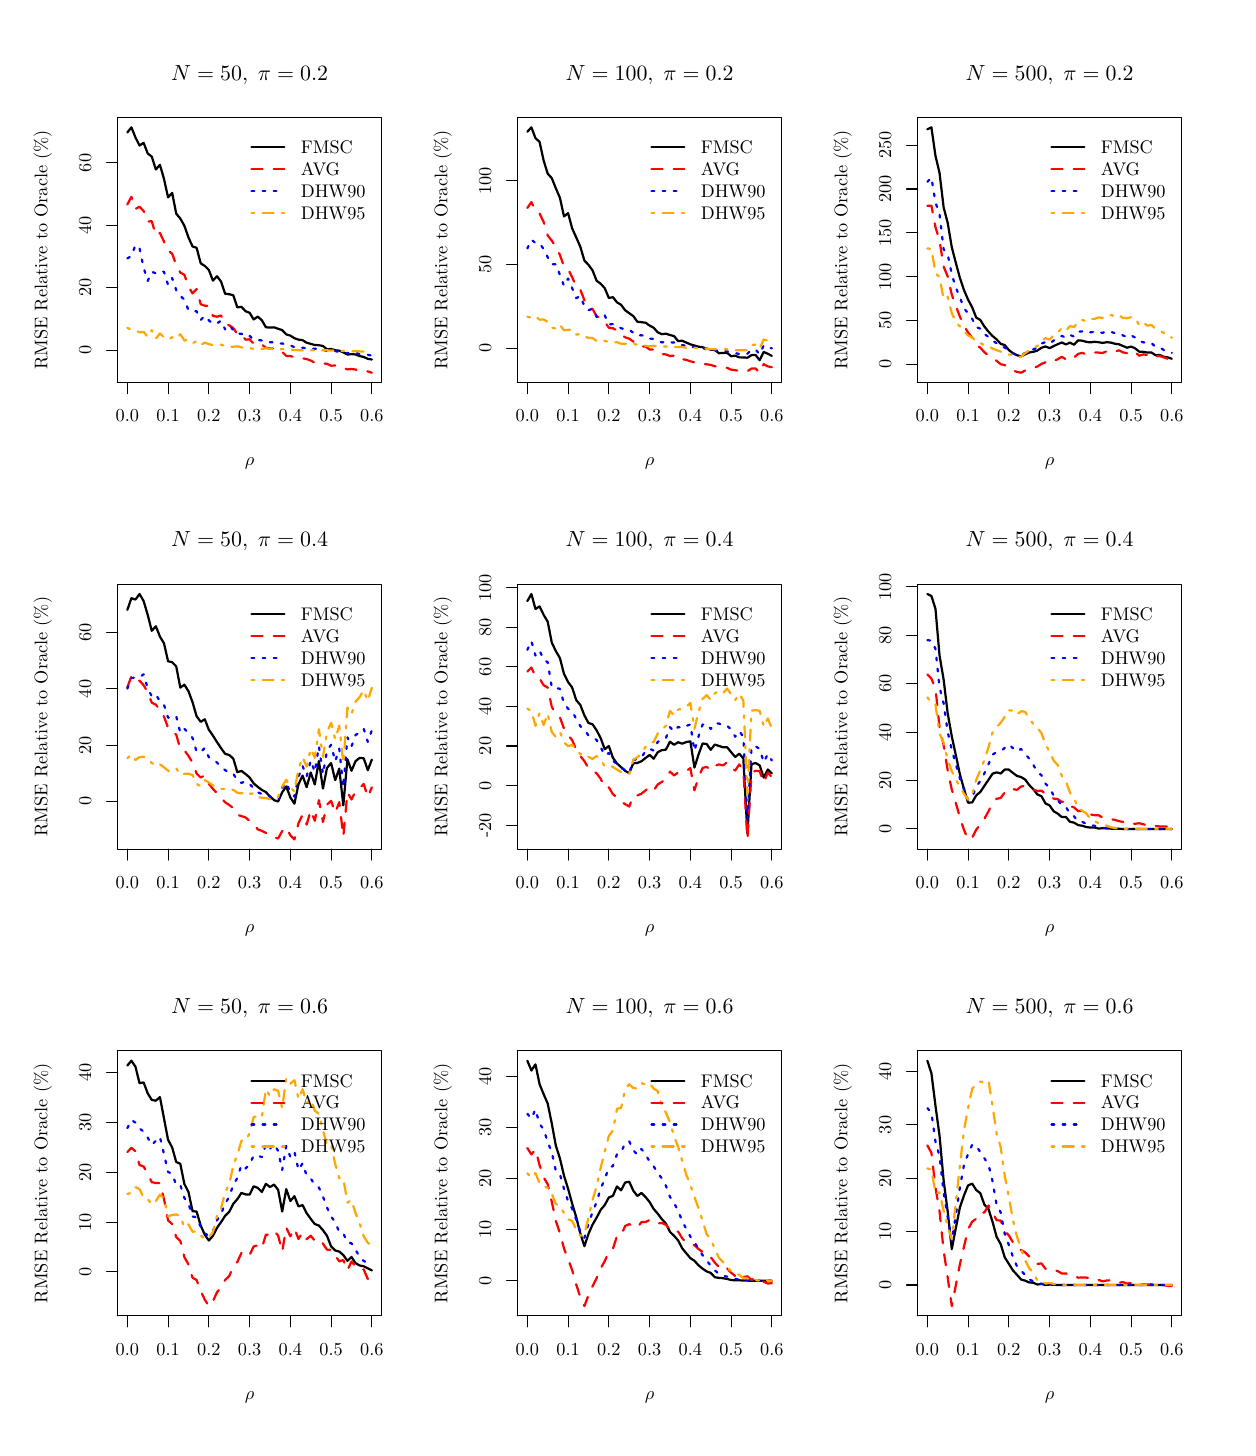
\begin{tikzpicture}[x=1pt,y=1pt]
\definecolor[named]{fillColor}{rgb}{1.00,1.00,1.00}
\path[use as bounding box,fill=fillColor,fill opacity=0.00] (0,0) rectangle (433.62,505.89);
\begin{scope}
\path[clip] ( 32.47,377.65) rectangle (127.91,473.42);
\definecolor[named]{drawColor}{rgb}{0.00,0.00,0.00}

\path[draw=drawColor,line width= 0.8pt,line join=round,line cap=round] ( 36.01,468.01) --
	( 37.48,469.87) --
	( 38.95,466.21) --
	( 40.42,463.29) --
	( 41.90,464.28) --
	( 43.37,460.43) --
	( 44.84,459.29) --
	( 46.32,454.63) --
	( 47.79,456.33) --
	( 49.26,451.21) --
	( 50.73,444.55) --
	( 52.21,446.18) --
	( 53.68,438.68) --
	( 55.15,436.91) --
	( 56.63,434.30) --
	( 58.10,430.10) --
	( 59.57,426.83) --
	( 61.04,426.35) --
	( 62.52,420.75) --
	( 63.99,419.80) --
	( 65.46,418.35) --
	( 66.93,414.49) --
	( 68.41,416.06) --
	( 69.88,414.12) --
	( 71.35,409.77) --
	( 72.83,409.56) --
	( 74.30,409.21) --
	( 75.77,404.81) --
	( 77.24,405.02) --
	( 78.72,403.44) --
	( 80.19,402.86) --
	( 81.66,400.46) --
	( 83.14,401.48) --
	( 84.61,400.16) --
	( 86.08,397.63) --
	( 87.55,397.50) --
	( 89.03,397.60) --
	( 90.50,397.10) --
	( 91.97,396.59) --
	( 93.44,395.05) --
	( 94.92,394.60) --
	( 96.39,393.68) --
	( 97.86,393.17) --
	( 99.34,392.96) --
	(100.81,392.04) --
	(102.28,391.63) --
	(103.75,391.21) --
	(105.23,391.15) --
	(106.70,390.86) --
	(108.17,389.69) --
	(109.65,389.78) --
	(111.12,389.32) --
	(112.59,389.17) --
	(114.06,388.58) --
	(115.54,387.75) --
	(117.01,387.93) --
	(118.48,387.80) --
	(119.95,387.22) --
	(121.43,386.90) --
	(122.90,386.22) --
	(124.37,385.98);
\end{scope}
\begin{scope}
\path[clip] (  0.00,  0.00) rectangle (433.62,505.89);
\definecolor[named]{drawColor}{rgb}{0.00,0.00,0.00}

\path[draw=drawColor,line width= 0.4pt,line join=round,line cap=round] ( 36.01,377.65) -- (124.37,377.65);

\path[draw=drawColor,line width= 0.4pt,line join=round,line cap=round] ( 36.01,377.65) -- ( 36.01,373.69);

\path[draw=drawColor,line width= 0.4pt,line join=round,line cap=round] ( 50.73,377.65) -- ( 50.73,373.69);

\path[draw=drawColor,line width= 0.4pt,line join=round,line cap=round] ( 65.46,377.65) -- ( 65.46,373.69);

\path[draw=drawColor,line width= 0.4pt,line join=round,line cap=round] ( 80.19,377.65) -- ( 80.19,373.69);

\path[draw=drawColor,line width= 0.4pt,line join=round,line cap=round] ( 94.92,377.65) -- ( 94.92,373.69);

\path[draw=drawColor,line width= 0.4pt,line join=round,line cap=round] (109.65,377.65) -- (109.65,373.69);

\path[draw=drawColor,line width= 0.4pt,line join=round,line cap=round] (124.37,377.65) -- (124.37,373.69);

\node[text=drawColor,anchor=base,inner sep=0pt, outer sep=0pt, scale=  0.66] at ( 36.01,363.40) {0.0};

\node[text=drawColor,anchor=base,inner sep=0pt, outer sep=0pt, scale=  0.66] at ( 50.73,363.40) {0.1};

\node[text=drawColor,anchor=base,inner sep=0pt, outer sep=0pt, scale=  0.66] at ( 65.46,363.40) {0.2};

\node[text=drawColor,anchor=base,inner sep=0pt, outer sep=0pt, scale=  0.66] at ( 80.19,363.40) {0.3};

\node[text=drawColor,anchor=base,inner sep=0pt, outer sep=0pt, scale=  0.66] at ( 94.92,363.40) {0.4};

\node[text=drawColor,anchor=base,inner sep=0pt, outer sep=0pt, scale=  0.66] at (109.65,363.40) {0.5};

\node[text=drawColor,anchor=base,inner sep=0pt, outer sep=0pt, scale=  0.66] at (124.37,363.40) {0.6};

\path[draw=drawColor,line width= 0.4pt,line join=round,line cap=round] ( 32.47,389.28) -- ( 32.47,457.03);

\path[draw=drawColor,line width= 0.4pt,line join=round,line cap=round] ( 32.47,389.28) -- ( 28.51,389.28);

\path[draw=drawColor,line width= 0.4pt,line join=round,line cap=round] ( 32.47,411.87) -- ( 28.51,411.87);

\path[draw=drawColor,line width= 0.4pt,line join=round,line cap=round] ( 32.47,434.45) -- ( 28.51,434.45);

\path[draw=drawColor,line width= 0.4pt,line join=round,line cap=round] ( 32.47,457.03) -- ( 28.51,457.03);

\node[text=drawColor,rotate= 90.00,anchor=base,inner sep=0pt, outer sep=0pt, scale=  0.66] at ( 22.97,389.28) {0};

\node[text=drawColor,rotate= 90.00,anchor=base,inner sep=0pt, outer sep=0pt, scale=  0.66] at ( 22.97,411.87) {20};

\node[text=drawColor,rotate= 90.00,anchor=base,inner sep=0pt, outer sep=0pt, scale=  0.66] at ( 22.97,434.45) {40};

\node[text=drawColor,rotate= 90.00,anchor=base,inner sep=0pt, outer sep=0pt, scale=  0.66] at ( 22.97,457.03) {60};

\path[draw=drawColor,line width= 0.4pt,line join=round,line cap=round] ( 32.47,377.65) --
	(127.91,377.65) --
	(127.91,473.42) --
	( 32.47,473.42) --
	( 32.47,377.65);
\end{scope}
\begin{scope}
\path[clip] (  0.00,337.26) rectangle (144.54,505.89);
\definecolor[named]{drawColor}{rgb}{0.00,0.00,0.00}

\node[text=drawColor,anchor=base,inner sep=0pt, outer sep=0pt, scale=  0.79] at ( 80.19,486.92) {\bfseries $N=50, \;\pi=0.2$};

\node[text=drawColor,anchor=base,inner sep=0pt, outer sep=0pt, scale=  0.66] at ( 80.19,347.56) {$\rho$};

\node[text=drawColor,rotate= 90.00,anchor=base,inner sep=0pt, outer sep=0pt, scale=  0.66] at (  7.13,425.53) {RMSE Relative to Oracle (\%)};
\end{scope}
\begin{scope}
\path[clip] ( 32.47,377.65) rectangle (127.91,473.42);
\definecolor[named]{drawColor}{rgb}{1.00,0.00,0.00}

\path[draw=drawColor,line width= 0.8pt,dash pattern=on 4pt off 4pt ,line join=round,line cap=round] ( 36.01,441.98) --
	( 37.48,444.78) --
	( 38.95,440.40) --
	( 40.42,441.19) --
	( 41.90,439.61) --
	( 43.37,435.81) --
	( 44.84,435.96) --
	( 46.32,430.84) --
	( 47.79,431.72) --
	( 49.26,428.56) --
	( 50.73,425.31) --
	( 52.21,424.23) --
	( 53.68,420.13) --
	( 55.15,417.39) --
	( 56.63,416.60) --
	( 58.10,412.30) --
	( 59.57,409.86) --
	( 61.04,411.46) --
	( 62.52,405.94) --
	( 63.99,405.42) --
	( 65.46,405.32) --
	( 66.93,401.76) --
	( 68.41,401.43) --
	( 69.88,401.89) --
	( 71.35,398.85) --
	( 72.83,398.34) --
	( 74.30,397.35) --
	( 75.77,395.17) --
	( 77.24,395.08) --
	( 78.72,393.13) --
	( 80.19,393.29) --
	( 81.66,391.67) --
	( 83.14,392.08) --
	( 84.61,391.39) --
	( 86.08,390.21) --
	( 87.55,389.99) --
	( 89.03,389.97) --
	( 90.50,389.63) --
	( 91.97,388.74) --
	( 93.44,387.29) --
	( 94.92,387.20) --
	( 96.39,386.83) --
	( 97.86,386.59) --
	( 99.34,386.42) --
	(100.81,386.13) --
	(102.28,385.61) --
	(103.75,384.81) --
	(105.23,384.93) --
	(106.70,384.59) --
	(108.17,384.42) --
	(109.65,383.73) --
	(111.12,383.83) --
	(112.59,383.59) --
	(114.06,383.01) --
	(115.54,382.39) --
	(117.01,382.56) --
	(118.48,382.36) --
	(119.95,381.77) --
	(121.43,381.84) --
	(122.90,381.68) --
	(124.37,381.20);
\definecolor[named]{drawColor}{rgb}{0.00,0.00,1.00}

\path[draw=drawColor,line width= 0.8pt,dash pattern=on 1pt off 3pt ,line join=round,line cap=round] ( 36.01,422.52) --
	( 37.48,423.31) --
	( 38.95,427.36) --
	( 40.42,426.16) --
	( 41.90,419.12) --
	( 43.37,414.37) --
	( 44.84,417.65) --
	( 46.32,417.13) --
	( 47.79,417.86) --
	( 49.26,417.68) --
	( 50.73,412.89) --
	( 52.21,415.41) --
	( 53.68,411.06) --
	( 55.15,408.94) --
	( 56.63,407.60) --
	( 58.10,403.81) --
	( 59.57,403.53) --
	( 61.04,403.40) --
	( 62.52,400.27) --
	( 63.99,401.73) --
	( 65.46,400.13) --
	( 66.93,398.80) --
	( 68.41,399.05) --
	( 69.88,399.98) --
	( 71.35,396.87) --
	( 72.83,398.37) --
	( 74.30,396.64) --
	( 75.77,395.26) --
	( 77.24,395.30) --
	( 78.72,394.22) --
	( 80.19,394.51) --
	( 81.66,393.13) --
	( 83.14,393.03) --
	( 84.61,392.86) --
	( 86.08,392.27) --
	( 87.55,392.23) --
	( 89.03,392.17) --
	( 90.50,391.79) --
	( 91.97,391.78) --
	( 93.44,391.40) --
	( 94.92,391.15) --
	( 96.39,390.41) --
	( 97.86,390.19) --
	( 99.34,390.22) --
	(100.81,390.07) --
	(102.28,390.02) --
	(103.75,389.86) --
	(105.23,389.86) --
	(106.70,389.45) --
	(108.17,389.10) --
	(109.65,389.05) --
	(111.12,389.05) --
	(112.59,388.65) --
	(114.06,388.43) --
	(115.54,388.31) --
	(117.01,388.31) --
	(118.48,388.42) --
	(119.95,387.91) --
	(121.43,387.71) --
	(122.90,387.66) --
	(124.37,387.36);
\definecolor[named]{drawColor}{rgb}{1.00,0.65,0.00}

\path[draw=drawColor,line width= 0.8pt,dash pattern=on 1pt off 3pt on 4pt off 3pt ,line join=round,line cap=round] ( 36.01,397.39) --
	( 37.48,396.77) --
	( 38.95,396.55) --
	( 40.42,395.76) --
	( 41.90,395.97) --
	( 43.37,394.11) --
	( 44.84,396.55) --
	( 46.32,393.49) --
	( 47.79,395.42) --
	( 49.26,394.00) --
	( 50.73,393.13) --
	( 52.21,394.03) --
	( 53.68,393.43) --
	( 55.15,395.10) --
	( 56.63,392.85) --
	( 58.10,393.08) --
	( 59.57,391.85) --
	( 61.04,392.61) --
	( 62.52,391.18) --
	( 63.99,392.08) --
	( 65.46,391.54) --
	( 66.93,391.19) --
	( 68.41,391.29) --
	( 69.88,391.33) --
	( 71.35,390.81) --
	( 72.83,390.63) --
	( 74.30,390.60) --
	( 75.77,390.74) --
	( 77.24,390.38) --
	( 78.72,390.07) --
	( 80.19,390.16) --
	( 81.66,389.82) --
	( 83.14,389.95) --
	( 84.61,389.78) --
	( 86.08,390.03) --
	( 87.55,389.88) --
	( 89.03,389.76) --
	( 90.50,389.59) --
	( 91.97,389.74) --
	( 93.44,389.69) --
	( 94.92,389.53) --
	( 96.39,389.43) --
	( 97.86,389.35) --
	( 99.34,389.30) --
	(100.81,389.38) --
	(102.28,389.32) --
	(103.75,389.29) --
	(105.23,389.22) --
	(106.70,389.30) --
	(108.17,389.32) --
	(109.65,389.18) --
	(111.12,389.28) --
	(112.59,389.09) --
	(114.06,389.05) --
	(115.54,389.10) --
	(117.01,388.98) --
	(118.48,388.99) --
	(119.95,388.91) --
	(121.43,388.84) --
	(122.90,388.79) --
	(124.37,388.74);
\definecolor[named]{drawColor}{rgb}{0.00,0.00,0.00}

\path[draw=drawColor,line width= 0.8pt,line join=round,line cap=round] ( 80.89,462.63) -- ( 92.77,462.63);
\definecolor[named]{drawColor}{rgb}{1.00,0.00,0.00}

\path[draw=drawColor,line width= 0.8pt,dash pattern=on 4pt off 4pt ,line join=round,line cap=round] ( 80.89,454.71) -- ( 92.77,454.71);
\definecolor[named]{drawColor}{rgb}{0.00,0.00,1.00}

\path[draw=drawColor,line width= 0.8pt,dash pattern=on 1pt off 3pt ,line join=round,line cap=round] ( 80.89,446.79) -- ( 92.77,446.79);
\definecolor[named]{drawColor}{rgb}{1.00,0.65,0.00}

\path[draw=drawColor,line width= 0.8pt,dash pattern=on 1pt off 3pt on 4pt off 3pt ,line join=round,line cap=round] ( 80.89,438.87) -- ( 92.77,438.87);
\definecolor[named]{drawColor}{rgb}{0.00,0.00,0.00}

\node[text=drawColor,anchor=base west,inner sep=0pt, outer sep=0pt, scale=  0.66] at ( 98.71,460.35) {FMSC};

\node[text=drawColor,anchor=base west,inner sep=0pt, outer sep=0pt, scale=  0.66] at ( 98.71,452.43) {AVG};

\node[text=drawColor,anchor=base west,inner sep=0pt, outer sep=0pt, scale=  0.66] at ( 98.71,444.51) {DHW90};

\node[text=drawColor,anchor=base west,inner sep=0pt, outer sep=0pt, scale=  0.66] at ( 98.71,436.59) {DHW95};
\end{scope}
\begin{scope}
\path[clip] (177.01,377.65) rectangle (272.45,473.42);
\definecolor[named]{drawColor}{rgb}{0.00,0.00,0.00}

\path[draw=drawColor,line width= 0.8pt,line join=round,line cap=round] (180.55,468.28) --
	(182.02,469.87) --
	(183.49,465.95) --
	(184.96,464.65) --
	(186.44,457.89) --
	(187.91,453.13) --
	(189.38,451.51) --
	(190.86,447.82) --
	(192.33,444.39) --
	(193.80,437.69) --
	(195.27,438.87) --
	(196.75,433.37) --
	(198.22,430.09) --
	(199.69,426.73) --
	(201.17,421.73) --
	(202.64,420.18) --
	(204.11,418.19) --
	(205.58,414.44) --
	(207.06,413.35) --
	(208.53,411.75) --
	(210.00,408.21) --
	(211.47,408.50) --
	(212.95,406.63) --
	(214.42,405.75) --
	(215.89,403.78) --
	(217.37,402.71) --
	(218.84,401.67) --
	(220.31,399.63) --
	(221.78,399.46) --
	(223.26,399.27) --
	(224.73,398.25) --
	(226.20,397.45) --
	(227.68,395.79) --
	(229.15,395.12) --
	(230.62,395.31) --
	(232.09,394.83) --
	(233.57,394.44) --
	(235.04,392.64) --
	(236.51,392.76) --
	(237.98,392.09) --
	(239.46,391.46) --
	(240.93,391.04) --
	(242.40,390.61) --
	(243.88,390.42) --
	(245.35,389.90) --
	(246.82,389.54) --
	(248.29,389.42) --
	(249.77,388.26) --
	(251.24,388.34) --
	(252.71,388.43) --
	(254.19,387.15) --
	(255.66,387.38) --
	(257.13,386.75) --
	(258.60,386.73) --
	(260.08,386.62) --
	(261.55,387.56) --
	(263.02,387.61) --
	(264.50,385.74) --
	(265.97,388.69) --
	(267.44,388.06) --
	(268.91,387.30);
\end{scope}
\begin{scope}
\path[clip] (  0.00,  0.00) rectangle (433.62,505.89);
\definecolor[named]{drawColor}{rgb}{0.00,0.00,0.00}

\path[draw=drawColor,line width= 0.4pt,line join=round,line cap=round] (180.55,377.65) -- (268.91,377.65);

\path[draw=drawColor,line width= 0.4pt,line join=round,line cap=round] (180.55,377.65) -- (180.55,373.69);

\path[draw=drawColor,line width= 0.4pt,line join=round,line cap=round] (195.27,377.65) -- (195.27,373.69);

\path[draw=drawColor,line width= 0.4pt,line join=round,line cap=round] (210.00,377.65) -- (210.00,373.69);

\path[draw=drawColor,line width= 0.4pt,line join=round,line cap=round] (224.73,377.65) -- (224.73,373.69);

\path[draw=drawColor,line width= 0.4pt,line join=round,line cap=round] (239.46,377.65) -- (239.46,373.69);

\path[draw=drawColor,line width= 0.4pt,line join=round,line cap=round] (254.19,377.65) -- (254.19,373.69);

\path[draw=drawColor,line width= 0.4pt,line join=round,line cap=round] (268.91,377.65) -- (268.91,373.69);

\node[text=drawColor,anchor=base,inner sep=0pt, outer sep=0pt, scale=  0.66] at (180.55,363.40) {0.0};

\node[text=drawColor,anchor=base,inner sep=0pt, outer sep=0pt, scale=  0.66] at (195.27,363.40) {0.1};

\node[text=drawColor,anchor=base,inner sep=0pt, outer sep=0pt, scale=  0.66] at (210.00,363.40) {0.2};

\node[text=drawColor,anchor=base,inner sep=0pt, outer sep=0pt, scale=  0.66] at (224.73,363.40) {0.3};

\node[text=drawColor,anchor=base,inner sep=0pt, outer sep=0pt, scale=  0.66] at (239.46,363.40) {0.4};

\node[text=drawColor,anchor=base,inner sep=0pt, outer sep=0pt, scale=  0.66] at (254.19,363.40) {0.5};

\node[text=drawColor,anchor=base,inner sep=0pt, outer sep=0pt, scale=  0.66] at (268.91,363.40) {0.6};

\path[draw=drawColor,line width= 0.4pt,line join=round,line cap=round] (177.01,390.04) -- (177.01,450.61);

\path[draw=drawColor,line width= 0.4pt,line join=round,line cap=round] (177.01,390.04) -- (173.05,390.04);

\path[draw=drawColor,line width= 0.4pt,line join=round,line cap=round] (177.01,420.33) -- (173.05,420.33);

\path[draw=drawColor,line width= 0.4pt,line join=round,line cap=round] (177.01,450.61) -- (173.05,450.61);

\node[text=drawColor,rotate= 90.00,anchor=base,inner sep=0pt, outer sep=0pt, scale=  0.66] at (167.51,390.04) {0};

\node[text=drawColor,rotate= 90.00,anchor=base,inner sep=0pt, outer sep=0pt, scale=  0.66] at (167.51,420.33) {50};

\node[text=drawColor,rotate= 90.00,anchor=base,inner sep=0pt, outer sep=0pt, scale=  0.66] at (167.51,450.61) {100};

\path[draw=drawColor,line width= 0.4pt,line join=round,line cap=round] (177.01,377.65) --
	(272.45,377.65) --
	(272.45,473.42) --
	(177.01,473.42) --
	(177.01,377.65);
\end{scope}
\begin{scope}
\path[clip] (144.54,337.26) rectangle (289.08,505.89);
\definecolor[named]{drawColor}{rgb}{0.00,0.00,0.00}

\node[text=drawColor,anchor=base,inner sep=0pt, outer sep=0pt, scale=  0.79] at (224.73,486.92) {\bfseries $N=100, \;\pi=0.2$};

\node[text=drawColor,anchor=base,inner sep=0pt, outer sep=0pt, scale=  0.66] at (224.73,347.56) {$\rho$};

\node[text=drawColor,rotate= 90.00,anchor=base,inner sep=0pt, outer sep=0pt, scale=  0.66] at (151.67,425.53) {RMSE Relative to Oracle (\%)};
\end{scope}
\begin{scope}
\path[clip] (177.01,377.65) rectangle (272.45,473.42);
\definecolor[named]{drawColor}{rgb}{1.00,0.00,0.00}

\path[draw=drawColor,line width= 0.8pt,dash pattern=on 4pt off 4pt ,line join=round,line cap=round] (180.55,440.74) --
	(182.02,442.87) --
	(183.49,439.53) --
	(184.96,438.79) --
	(186.44,435.68) --
	(187.91,430.79) --
	(189.38,428.94) --
	(190.86,426.65) --
	(192.33,423.73) --
	(193.80,419.58) --
	(195.27,418.65) --
	(196.75,415.73) --
	(198.22,412.28) --
	(199.69,411.21) --
	(201.17,407.40) --
	(202.64,405.02) --
	(204.11,404.22) --
	(205.58,401.67) --
	(207.06,400.87) --
	(208.53,399.56) --
	(210.00,397.47) --
	(211.47,397.27) --
	(212.95,396.47) --
	(214.42,395.03) --
	(215.89,394.00) --
	(217.37,393.49) --
	(218.84,392.49) --
	(220.31,390.98) --
	(221.78,390.64) --
	(223.26,390.70) --
	(224.73,389.58) --
	(226.20,389.57) --
	(227.68,388.51) --
	(229.15,387.99) --
	(230.62,387.80) --
	(232.09,387.26) --
	(233.57,387.37) --
	(235.04,386.11) --
	(236.51,386.08) --
	(237.98,385.86) --
	(239.46,385.33) --
	(240.93,384.96) --
	(242.40,384.50) --
	(243.88,384.33) --
	(245.35,384.25) --
	(246.82,384.01) --
	(248.29,383.56) --
	(249.77,383.20) --
	(251.24,383.03) --
	(252.71,382.96) --
	(254.19,382.31) --
	(255.66,382.13) --
	(257.13,381.83) --
	(258.60,381.80) --
	(260.08,381.72) --
	(261.55,382.71) --
	(263.02,382.75) --
	(264.50,381.20) --
	(265.97,384.28) --
	(267.44,383.48) --
	(268.91,383.20);
\definecolor[named]{drawColor}{rgb}{0.00,0.00,1.00}

\path[draw=drawColor,line width= 0.8pt,dash pattern=on 1pt off 3pt ,line join=round,line cap=round] (180.55,426.11) --
	(182.02,429.26) --
	(183.49,428.07) --
	(184.96,427.93) --
	(186.44,425.90) --
	(187.91,422.89) --
	(189.38,420.35) --
	(190.86,420.41) --
	(192.33,416.53) --
	(193.80,412.58) --
	(195.27,415.23) --
	(196.75,411.74) --
	(198.22,408.17) --
	(199.69,408.94) --
	(201.17,405.24) --
	(202.64,403.75) --
	(204.11,404.37) --
	(205.58,401.38) --
	(207.06,401.06) --
	(208.53,401.88) --
	(210.00,398.69) --
	(211.47,398.78) --
	(212.95,398.20) --
	(214.42,397.27) --
	(215.89,396.90) --
	(217.37,396.78) --
	(218.84,395.63) --
	(220.31,394.49) --
	(221.78,394.78) --
	(223.26,394.26) --
	(224.73,393.55) --
	(226.20,393.39) --
	(227.68,392.73) --
	(229.15,392.15) --
	(230.62,392.36) --
	(232.09,392.16) --
	(233.57,392.15) --
	(235.04,391.16) --
	(236.51,391.15) --
	(237.98,390.95) --
	(239.46,390.51) --
	(240.93,390.45) --
	(242.40,390.38) --
	(243.88,390.16) --
	(245.35,389.62) --
	(246.82,389.62) --
	(248.29,389.35) --
	(249.77,389.05) --
	(251.24,388.99) --
	(252.71,388.90) --
	(254.19,388.40) --
	(255.66,388.29) --
	(257.13,387.98) --
	(258.60,387.89) --
	(260.08,388.09) --
	(261.55,389.48) --
	(263.02,389.55) --
	(264.50,387.89) --
	(265.97,391.07) --
	(267.44,390.42) --
	(268.91,390.02);
\definecolor[named]{drawColor}{rgb}{1.00,0.65,0.00}

\path[draw=drawColor,line width= 0.8pt,dash pattern=on 1pt off 3pt on 4pt off 3pt ,line join=round,line cap=round] (180.55,401.48) --
	(182.02,401.08) --
	(183.49,401.65) --
	(184.96,400.37) --
	(186.44,400.43) --
	(187.91,399.57) --
	(189.38,397.48) --
	(190.86,397.13) --
	(192.33,398.51) --
	(193.80,396.52) --
	(195.27,396.73) --
	(196.75,396.81) --
	(198.22,395.00) --
	(199.69,395.19) --
	(201.17,394.32) --
	(202.64,393.81) --
	(204.11,393.76) --
	(205.58,392.64) --
	(207.06,392.90) --
	(208.53,392.66) --
	(210.00,392.40) --
	(211.47,392.11) --
	(212.95,392.20) --
	(214.42,391.72) --
	(215.89,391.64) --
	(217.37,391.98) --
	(218.84,391.74) --
	(220.31,391.27) --
	(221.78,391.49) --
	(223.26,390.94) --
	(224.73,390.74) --
	(226.20,390.95) --
	(227.68,390.74) --
	(229.15,390.65) --
	(230.62,390.71) --
	(232.09,390.60) --
	(233.57,390.48) --
	(235.04,390.51) --
	(236.51,390.48) --
	(237.98,390.20) --
	(239.46,390.28) --
	(240.93,390.19) --
	(242.40,390.02) --
	(243.88,390.10) --
	(245.35,389.85) --
	(246.82,389.79) --
	(248.29,389.69) --
	(249.77,389.66) --
	(251.24,389.64) --
	(252.71,389.65) --
	(254.19,389.52) --
	(255.66,389.32) --
	(257.13,389.29) --
	(258.60,389.33) --
	(260.08,389.32) --
	(261.55,391.16) --
	(263.02,391.38) --
	(264.50,389.87) --
	(265.97,393.26) --
	(267.44,392.75) --
	(268.91,392.61);
\definecolor[named]{drawColor}{rgb}{0.00,0.00,0.00}

\path[draw=drawColor,line width= 0.8pt,line join=round,line cap=round] (225.43,462.63) -- (237.31,462.63);
\definecolor[named]{drawColor}{rgb}{1.00,0.00,0.00}

\path[draw=drawColor,line width= 0.8pt,dash pattern=on 4pt off 4pt ,line join=round,line cap=round] (225.43,454.71) -- (237.31,454.71);
\definecolor[named]{drawColor}{rgb}{0.00,0.00,1.00}

\path[draw=drawColor,line width= 0.8pt,dash pattern=on 1pt off 3pt ,line join=round,line cap=round] (225.43,446.79) -- (237.31,446.79);
\definecolor[named]{drawColor}{rgb}{1.00,0.65,0.00}

\path[draw=drawColor,line width= 0.8pt,dash pattern=on 1pt off 3pt on 4pt off 3pt ,line join=round,line cap=round] (225.43,438.87) -- (237.31,438.87);
\definecolor[named]{drawColor}{rgb}{0.00,0.00,0.00}

\node[text=drawColor,anchor=base west,inner sep=0pt, outer sep=0pt, scale=  0.66] at (243.25,460.35) {FMSC};

\node[text=drawColor,anchor=base west,inner sep=0pt, outer sep=0pt, scale=  0.66] at (243.25,452.43) {AVG};

\node[text=drawColor,anchor=base west,inner sep=0pt, outer sep=0pt, scale=  0.66] at (243.25,444.51) {DHW90};

\node[text=drawColor,anchor=base west,inner sep=0pt, outer sep=0pt, scale=  0.66] at (243.25,436.59) {DHW95};
\end{scope}
\begin{scope}
\path[clip] (321.55,377.65) rectangle (416.99,473.42);
\definecolor[named]{drawColor}{rgb}{0.00,0.00,0.00}

\path[draw=drawColor,line width= 0.8pt,line join=round,line cap=round] (325.09,469.16) --
	(326.56,469.87) --
	(328.03,459.59) --
	(329.50,453.38) --
	(330.98,440.93) --
	(332.45,435.35) --
	(333.92,426.58) --
	(335.40,420.84) --
	(336.87,415.40) --
	(338.34,411.02) --
	(339.81,407.63) --
	(341.29,404.84) --
	(342.76,401.12) --
	(344.23,400.27) --
	(345.71,397.87) --
	(347.18,396.05) --
	(348.65,394.45) --
	(350.12,393.25) --
	(351.60,391.64) --
	(353.07,391.20) --
	(354.54,389.39) --
	(356.01,388.26) --
	(357.49,387.52) --
	(358.96,387.13) --
	(360.43,387.83) --
	(361.91,388.51) --
	(363.38,388.76) --
	(364.85,389.20) --
	(366.32,390.22) --
	(367.80,390.68) --
	(369.27,390.09) --
	(370.74,390.81) --
	(372.22,391.53) --
	(373.69,392.12) --
	(375.16,391.43) --
	(376.63,392.07) --
	(378.11,391.33) --
	(379.58,392.90) --
	(381.05,392.77) --
	(382.52,392.35) --
	(384.00,392.17) --
	(385.47,392.38) --
	(386.94,392.23) --
	(388.42,391.97) --
	(389.89,392.22) --
	(391.36,392.11) --
	(392.83,391.68) --
	(394.31,391.48) --
	(395.78,390.87) --
	(397.25,390.24) --
	(398.73,390.66) --
	(400.20,389.99) --
	(401.67,388.80) --
	(403.14,388.74) --
	(404.62,388.50) --
	(406.09,388.51) --
	(407.56,387.52) --
	(409.04,387.60) --
	(410.51,386.99) --
	(411.98,386.73) --
	(413.45,386.24);
\end{scope}
\begin{scope}
\path[clip] (  0.00,  0.00) rectangle (433.62,505.89);
\definecolor[named]{drawColor}{rgb}{0.00,0.00,0.00}

\path[draw=drawColor,line width= 0.4pt,line join=round,line cap=round] (325.09,377.65) -- (413.45,377.65);

\path[draw=drawColor,line width= 0.4pt,line join=round,line cap=round] (325.09,377.65) -- (325.09,373.69);

\path[draw=drawColor,line width= 0.4pt,line join=round,line cap=round] (339.81,377.65) -- (339.81,373.69);

\path[draw=drawColor,line width= 0.4pt,line join=round,line cap=round] (354.54,377.65) -- (354.54,373.69);

\path[draw=drawColor,line width= 0.4pt,line join=round,line cap=round] (369.27,377.65) -- (369.27,373.69);

\path[draw=drawColor,line width= 0.4pt,line join=round,line cap=round] (384.00,377.65) -- (384.00,373.69);

\path[draw=drawColor,line width= 0.4pt,line join=round,line cap=round] (398.73,377.65) -- (398.73,373.69);

\path[draw=drawColor,line width= 0.4pt,line join=round,line cap=round] (413.45,377.65) -- (413.45,373.69);

\node[text=drawColor,anchor=base,inner sep=0pt, outer sep=0pt, scale=  0.66] at (325.09,363.40) {0.0};

\node[text=drawColor,anchor=base,inner sep=0pt, outer sep=0pt, scale=  0.66] at (339.81,363.40) {0.1};

\node[text=drawColor,anchor=base,inner sep=0pt, outer sep=0pt, scale=  0.66] at (354.54,363.40) {0.2};

\node[text=drawColor,anchor=base,inner sep=0pt, outer sep=0pt, scale=  0.66] at (369.27,363.40) {0.3};

\node[text=drawColor,anchor=base,inner sep=0pt, outer sep=0pt, scale=  0.66] at (384.00,363.40) {0.4};

\node[text=drawColor,anchor=base,inner sep=0pt, outer sep=0pt, scale=  0.66] at (398.73,363.40) {0.5};

\node[text=drawColor,anchor=base,inner sep=0pt, outer sep=0pt, scale=  0.66] at (413.45,363.40) {0.6};

\path[draw=drawColor,line width= 0.4pt,line join=round,line cap=round] (321.55,384.22) -- (321.55,463.40);

\path[draw=drawColor,line width= 0.4pt,line join=round,line cap=round] (321.55,384.22) -- (317.59,384.22);

\path[draw=drawColor,line width= 0.4pt,line join=round,line cap=round] (321.55,400.06) -- (317.59,400.06);

\path[draw=drawColor,line width= 0.4pt,line join=round,line cap=round] (321.55,415.89) -- (317.59,415.89);

\path[draw=drawColor,line width= 0.4pt,line join=round,line cap=round] (321.55,431.73) -- (317.59,431.73);

\path[draw=drawColor,line width= 0.4pt,line join=round,line cap=round] (321.55,447.57) -- (317.59,447.57);

\path[draw=drawColor,line width= 0.4pt,line join=round,line cap=round] (321.55,463.40) -- (317.59,463.40);

\node[text=drawColor,rotate= 90.00,anchor=base,inner sep=0pt, outer sep=0pt, scale=  0.66] at (312.05,384.22) {0};

\node[text=drawColor,rotate= 90.00,anchor=base,inner sep=0pt, outer sep=0pt, scale=  0.66] at (312.05,400.06) {50};

\node[text=drawColor,rotate= 90.00,anchor=base,inner sep=0pt, outer sep=0pt, scale=  0.66] at (312.05,415.89) {100};

\node[text=drawColor,rotate= 90.00,anchor=base,inner sep=0pt, outer sep=0pt, scale=  0.66] at (312.05,431.73) {150};

\node[text=drawColor,rotate= 90.00,anchor=base,inner sep=0pt, outer sep=0pt, scale=  0.66] at (312.05,447.57) {200};

\node[text=drawColor,rotate= 90.00,anchor=base,inner sep=0pt, outer sep=0pt, scale=  0.66] at (312.05,463.40) {250};

\path[draw=drawColor,line width= 0.4pt,line join=round,line cap=round] (321.55,377.65) --
	(416.99,377.65) --
	(416.99,473.42) --
	(321.55,473.42) --
	(321.55,377.65);
\end{scope}
\begin{scope}
\path[clip] (289.08,337.26) rectangle (433.62,505.89);
\definecolor[named]{drawColor}{rgb}{0.00,0.00,0.00}

\node[text=drawColor,anchor=base,inner sep=0pt, outer sep=0pt, scale=  0.79] at (369.27,486.92) {\bfseries $N=500, \;\pi=0.2$};

\node[text=drawColor,anchor=base,inner sep=0pt, outer sep=0pt, scale=  0.66] at (369.27,347.56) {$\rho$};

\node[text=drawColor,rotate= 90.00,anchor=base,inner sep=0pt, outer sep=0pt, scale=  0.66] at (296.21,425.53) {RMSE Relative to Oracle (\%)};
\end{scope}
\begin{scope}
\path[clip] (321.55,377.65) rectangle (416.99,473.42);
\definecolor[named]{drawColor}{rgb}{1.00,0.00,0.00}

\path[draw=drawColor,line width= 0.8pt,dash pattern=on 4pt off 4pt ,line join=round,line cap=round] (325.09,441.49) --
	(326.56,441.58) --
	(328.03,433.82) --
	(329.50,428.96) --
	(330.98,419.55) --
	(332.45,415.99) --
	(333.92,409.42) --
	(335.40,405.29) --
	(336.87,401.43) --
	(338.34,398.13) --
	(339.81,395.73) --
	(341.29,393.86) --
	(342.76,391.17) --
	(344.23,390.26) --
	(345.71,388.60) --
	(347.18,387.49) --
	(348.65,386.35) --
	(350.12,385.50) --
	(351.60,384.29) --
	(353.07,383.94) --
	(354.54,382.74) --
	(356.01,381.97) --
	(357.49,381.52) --
	(358.96,381.20) --
	(360.43,382.02) --
	(361.91,382.58) --
	(363.38,382.93) --
	(364.85,383.44) --
	(366.32,384.39) --
	(367.80,384.99) --
	(369.27,384.60) --
	(370.74,385.38) --
	(372.22,386.11) --
	(373.69,386.96) --
	(375.16,386.04) --
	(376.63,387.12) --
	(378.11,386.70) --
	(379.58,388.01) --
	(381.05,388.38) --
	(382.52,387.84) --
	(384.00,388.24) --
	(385.47,388.48) --
	(386.94,388.47) --
	(388.42,388.34) --
	(389.89,388.97) --
	(391.36,389.09) --
	(392.83,388.74) --
	(394.31,389.31) --
	(395.78,388.55) --
	(397.25,388.29) --
	(398.73,389.00) --
	(400.20,388.65) --
	(401.67,387.34) --
	(403.14,387.85) --
	(404.62,387.61) --
	(406.09,388.12) --
	(407.56,387.14) --
	(409.04,387.24) --
	(410.51,386.75) --
	(411.98,386.23) --
	(413.45,386.30);
\definecolor[named]{drawColor}{rgb}{0.00,0.00,1.00}

\path[draw=drawColor,line width= 0.8pt,dash pattern=on 1pt off 3pt ,line join=round,line cap=round] (325.09,450.17) --
	(326.56,451.74) --
	(328.03,442.77) --
	(329.50,438.44) --
	(330.98,425.75) --
	(332.45,424.00) --
	(333.92,416.73) --
	(335.40,411.95) --
	(336.87,408.38) --
	(338.34,404.46) --
	(339.81,402.68) --
	(341.29,400.68) --
	(342.76,397.67) --
	(344.23,397.13) --
	(345.71,395.14) --
	(347.18,394.16) --
	(348.65,392.81) --
	(350.12,391.83) --
	(351.60,390.73) --
	(353.07,390.30) --
	(354.54,389.05) --
	(356.01,388.22) --
	(357.49,387.60) --
	(358.96,387.46) --
	(360.43,388.35) --
	(361.91,389.14) --
	(363.38,389.63) --
	(364.85,390.27) --
	(366.32,391.74) --
	(367.80,392.28) --
	(369.27,391.68) --
	(370.74,392.84) --
	(372.22,393.47) --
	(373.69,394.53) --
	(375.16,393.82) --
	(376.63,394.84) --
	(378.11,394.28) --
	(379.58,396.02) --
	(381.05,396.11) --
	(382.52,395.56) --
	(384.00,395.79) --
	(385.47,396.02) --
	(386.94,395.84) --
	(388.42,395.62) --
	(389.89,396.18) --
	(391.36,396.03) --
	(392.83,395.47) --
	(394.31,395.47) --
	(395.78,394.68) --
	(397.25,394.07) --
	(398.73,394.69) --
	(400.20,393.89) --
	(401.67,392.57) --
	(403.14,392.21) --
	(404.62,391.80) --
	(406.09,391.90) --
	(407.56,390.50) --
	(409.04,390.36) --
	(410.51,389.43) --
	(411.98,388.89) --
	(413.45,388.41);
\definecolor[named]{drawColor}{rgb}{1.00,0.65,0.00}

\path[draw=drawColor,line width= 0.8pt,dash pattern=on 1pt off 3pt on 4pt off 3pt ,line join=round,line cap=round] (325.09,426.14) --
	(326.56,425.91) --
	(328.03,417.32) --
	(329.50,415.68) --
	(330.98,407.76) --
	(332.45,408.62) --
	(333.92,402.71) --
	(335.40,399.54) --
	(336.87,397.91) --
	(338.34,396.11) --
	(339.81,394.67) --
	(341.29,394.00) --
	(342.76,392.21) --
	(344.23,391.94) --
	(345.71,391.11) --
	(347.18,390.87) --
	(348.65,389.92) --
	(350.12,389.36) --
	(351.60,388.83) --
	(353.07,388.65) --
	(354.54,387.82) --
	(356.01,387.55) --
	(357.49,386.86) --
	(358.96,386.99) --
	(360.43,388.25) --
	(361.91,389.24) --
	(363.38,390.18) --
	(364.85,390.88) --
	(366.32,392.72) --
	(367.80,393.70) --
	(369.27,393.15) --
	(370.74,394.78) --
	(372.22,395.77) --
	(373.69,397.30) --
	(375.16,396.39) --
	(376.63,398.07) --
	(378.11,397.70) --
	(379.58,399.68) --
	(381.05,400.32) --
	(382.52,399.75) --
	(384.00,400.67) --
	(385.47,400.65) --
	(386.94,401.19) --
	(388.42,401.03) --
	(389.89,401.89) --
	(391.36,402.10) --
	(392.83,401.56) --
	(394.31,402.07) --
	(395.78,401.00) --
	(397.25,400.90) --
	(398.73,401.26) --
	(400.20,400.89) --
	(401.67,398.41) --
	(403.14,399.32) --
	(404.62,398.19) --
	(406.09,398.48) --
	(407.56,397.08) --
	(409.04,396.42) --
	(410.51,395.58) --
	(411.98,394.26) --
	(413.45,393.88);
\definecolor[named]{drawColor}{rgb}{0.00,0.00,0.00}

\path[draw=drawColor,line width= 0.8pt,line join=round,line cap=round] (369.97,462.63) -- (381.85,462.63);
\definecolor[named]{drawColor}{rgb}{1.00,0.00,0.00}

\path[draw=drawColor,line width= 0.8pt,dash pattern=on 4pt off 4pt ,line join=round,line cap=round] (369.97,454.71) -- (381.85,454.71);
\definecolor[named]{drawColor}{rgb}{0.00,0.00,1.00}

\path[draw=drawColor,line width= 0.8pt,dash pattern=on 1pt off 3pt ,line join=round,line cap=round] (369.97,446.79) -- (381.85,446.79);
\definecolor[named]{drawColor}{rgb}{1.00,0.65,0.00}

\path[draw=drawColor,line width= 0.8pt,dash pattern=on 1pt off 3pt on 4pt off 3pt ,line join=round,line cap=round] (369.97,438.87) -- (381.85,438.87);
\definecolor[named]{drawColor}{rgb}{0.00,0.00,0.00}

\node[text=drawColor,anchor=base west,inner sep=0pt, outer sep=0pt, scale=  0.66] at (387.79,460.35) {FMSC};

\node[text=drawColor,anchor=base west,inner sep=0pt, outer sep=0pt, scale=  0.66] at (387.79,452.43) {AVG};

\node[text=drawColor,anchor=base west,inner sep=0pt, outer sep=0pt, scale=  0.66] at (387.79,444.51) {DHW90};

\node[text=drawColor,anchor=base west,inner sep=0pt, outer sep=0pt, scale=  0.66] at (387.79,436.59) {DHW95};
\end{scope}
\begin{scope}
\path[clip] ( 32.47,209.02) rectangle (127.91,304.79);
\definecolor[named]{drawColor}{rgb}{0.00,0.00,0.00}

\path[draw=drawColor,line width= 0.8pt,line join=round,line cap=round] ( 36.01,295.49) --
	( 37.48,299.75) --
	( 38.95,299.25) --
	( 40.42,301.24) --
	( 41.90,298.69) --
	( 43.37,293.73) --
	( 44.84,287.94) --
	( 46.32,289.59) --
	( 47.79,285.84) --
	( 49.26,283.42) --
	( 50.73,276.94) --
	( 52.21,276.59) --
	( 53.68,275.08) --
	( 55.15,267.43) --
	( 56.63,268.47) --
	( 58.10,266.12) --
	( 59.57,262.14) --
	( 61.04,257.09) --
	( 62.52,255.05) --
	( 63.99,255.98) --
	( 65.46,252.21) --
	( 66.93,250.09) --
	( 68.41,247.72) --
	( 69.88,245.53) --
	( 71.35,243.49) --
	( 72.83,243.06) --
	( 74.30,241.76) --
	( 75.77,236.85) --
	( 77.24,237.33) --
	( 78.72,236.20) --
	( 80.19,234.94) --
	( 81.66,232.80) --
	( 83.14,231.57) --
	( 84.61,230.44) --
	( 86.08,229.66) --
	( 87.55,228.06) --
	( 89.03,226.77) --
	( 90.50,226.25) --
	( 91.97,229.60) --
	( 93.44,231.70) --
	( 94.92,227.73) --
	( 96.39,225.47) --
	( 97.86,232.51) --
	( 99.34,235.63) --
	(100.81,231.44) --
	(102.28,236.75) --
	(103.75,232.42) --
	(105.23,240.91) --
	(106.70,230.95) --
	(108.17,238.41) --
	(109.65,240.17) --
	(111.12,233.98) --
	(112.59,238.12) --
	(114.06,224.87) --
	(115.54,241.54) --
	(117.01,237.36) --
	(118.48,240.85) --
	(119.95,242.02) --
	(121.43,241.88) --
	(122.90,237.58) --
	(124.37,241.42);
\end{scope}
\begin{scope}
\path[clip] (  0.00,  0.00) rectangle (433.62,505.89);
\definecolor[named]{drawColor}{rgb}{0.00,0.00,0.00}

\path[draw=drawColor,line width= 0.4pt,line join=round,line cap=round] ( 36.01,209.02) -- (124.37,209.02);

\path[draw=drawColor,line width= 0.4pt,line join=round,line cap=round] ( 36.01,209.02) -- ( 36.01,205.06);

\path[draw=drawColor,line width= 0.4pt,line join=round,line cap=round] ( 50.73,209.02) -- ( 50.73,205.06);

\path[draw=drawColor,line width= 0.4pt,line join=round,line cap=round] ( 65.46,209.02) -- ( 65.46,205.06);

\path[draw=drawColor,line width= 0.4pt,line join=round,line cap=round] ( 80.19,209.02) -- ( 80.19,205.06);

\path[draw=drawColor,line width= 0.4pt,line join=round,line cap=round] ( 94.92,209.02) -- ( 94.92,205.06);

\path[draw=drawColor,line width= 0.4pt,line join=round,line cap=round] (109.65,209.02) -- (109.65,205.06);

\path[draw=drawColor,line width= 0.4pt,line join=round,line cap=round] (124.37,209.02) -- (124.37,205.06);

\node[text=drawColor,anchor=base,inner sep=0pt, outer sep=0pt, scale=  0.66] at ( 36.01,194.77) {0.0};

\node[text=drawColor,anchor=base,inner sep=0pt, outer sep=0pt, scale=  0.66] at ( 50.73,194.77) {0.1};

\node[text=drawColor,anchor=base,inner sep=0pt, outer sep=0pt, scale=  0.66] at ( 65.46,194.77) {0.2};

\node[text=drawColor,anchor=base,inner sep=0pt, outer sep=0pt, scale=  0.66] at ( 80.19,194.77) {0.3};

\node[text=drawColor,anchor=base,inner sep=0pt, outer sep=0pt, scale=  0.66] at ( 94.92,194.77) {0.4};

\node[text=drawColor,anchor=base,inner sep=0pt, outer sep=0pt, scale=  0.66] at (109.65,194.77) {0.5};

\node[text=drawColor,anchor=base,inner sep=0pt, outer sep=0pt, scale=  0.66] at (124.37,194.77) {0.6};

\path[draw=drawColor,line width= 0.4pt,line join=round,line cap=round] ( 32.47,226.33) -- ( 32.47,287.28);

\path[draw=drawColor,line width= 0.4pt,line join=round,line cap=round] ( 32.47,226.33) -- ( 28.51,226.33);

\path[draw=drawColor,line width= 0.4pt,line join=round,line cap=round] ( 32.47,246.65) -- ( 28.51,246.65);

\path[draw=drawColor,line width= 0.4pt,line join=round,line cap=round] ( 32.47,266.96) -- ( 28.51,266.96);

\path[draw=drawColor,line width= 0.4pt,line join=round,line cap=round] ( 32.47,287.28) -- ( 28.51,287.28);

\node[text=drawColor,rotate= 90.00,anchor=base,inner sep=0pt, outer sep=0pt, scale=  0.66] at ( 22.97,226.33) {0};

\node[text=drawColor,rotate= 90.00,anchor=base,inner sep=0pt, outer sep=0pt, scale=  0.66] at ( 22.97,246.65) {20};

\node[text=drawColor,rotate= 90.00,anchor=base,inner sep=0pt, outer sep=0pt, scale=  0.66] at ( 22.97,266.96) {40};

\node[text=drawColor,rotate= 90.00,anchor=base,inner sep=0pt, outer sep=0pt, scale=  0.66] at ( 22.97,287.28) {60};

\path[draw=drawColor,line width= 0.4pt,line join=round,line cap=round] ( 32.47,209.02) --
	(127.91,209.02) --
	(127.91,304.79) --
	( 32.47,304.79) --
	( 32.47,209.02);
\end{scope}
\begin{scope}
\path[clip] (  0.00,168.63) rectangle (144.54,337.26);
\definecolor[named]{drawColor}{rgb}{0.00,0.00,0.00}

\node[text=drawColor,anchor=base,inner sep=0pt, outer sep=0pt, scale=  0.79] at ( 80.19,318.29) {\bfseries $N=50, \;\pi=0.4$};

\node[text=drawColor,anchor=base,inner sep=0pt, outer sep=0pt, scale=  0.66] at ( 80.19,178.93) {$\rho$};

\node[text=drawColor,rotate= 90.00,anchor=base,inner sep=0pt, outer sep=0pt, scale=  0.66] at (  7.13,256.90) {RMSE Relative to Oracle (\%)};
\end{scope}
\begin{scope}
\path[clip] ( 32.47,209.02) rectangle (127.91,304.79);
\definecolor[named]{drawColor}{rgb}{1.00,0.00,0.00}

\path[draw=drawColor,line width= 0.8pt,dash pattern=on 4pt off 4pt ,line join=round,line cap=round] ( 36.01,267.48) --
	( 37.48,271.53) --
	( 38.95,269.63) --
	( 40.42,269.93) --
	( 41.90,268.27) --
	( 43.37,265.78) --
	( 44.84,261.97) --
	( 46.32,261.26) --
	( 47.79,259.21) --
	( 49.26,256.93) --
	( 50.73,252.90) --
	( 52.21,251.37) --
	( 53.68,250.44) --
	( 55.15,245.22) --
	( 56.63,244.78) --
	( 58.10,242.74) --
	( 59.57,240.39) --
	( 61.04,236.37) --
	( 62.52,234.93) --
	( 63.99,235.65) --
	( 65.46,232.63) --
	( 66.93,230.84) --
	( 68.41,229.22) --
	( 69.88,227.53) --
	( 71.35,225.99) --
	( 72.83,224.99) --
	( 74.30,223.83) --
	( 75.77,221.43) --
	( 77.24,221.00) --
	( 78.72,220.51) --
	( 80.19,219.25) --
	( 81.66,218.06) --
	( 83.14,216.21) --
	( 84.61,215.67) --
	( 86.08,214.92) --
	( 87.55,213.86) --
	( 89.03,213.32) --
	( 90.50,212.90) --
	( 91.97,215.58) --
	( 93.44,216.91) --
	( 94.92,214.01) --
	( 96.39,212.57) --
	( 97.86,218.46) --
	( 99.34,221.48) --
	(100.81,217.94) --
	(102.28,223.06) --
	(103.75,219.31) --
	(105.23,226.74) --
	(106.70,218.85) --
	(108.17,225.16) --
	(109.65,226.50) --
	(111.12,222.18) --
	(112.59,226.06) --
	(114.06,213.66) --
	(115.54,229.55) --
	(117.01,227.01) --
	(118.48,229.94) --
	(119.95,231.02) --
	(121.43,232.60) --
	(122.90,227.87) --
	(124.37,231.39);
\definecolor[named]{drawColor}{rgb}{0.00,0.00,1.00}

\path[draw=drawColor,line width= 0.8pt,dash pattern=on 1pt off 3pt ,line join=round,line cap=round] ( 36.01,267.04) --
	( 37.48,270.88) --
	( 38.95,271.05) --
	( 40.42,271.18) --
	( 41.90,272.23) --
	( 43.37,267.16) --
	( 44.84,264.31) --
	( 46.32,264.97) --
	( 47.79,262.41) --
	( 49.26,261.19) --
	( 50.73,256.53) --
	( 52.21,256.84) --
	( 53.68,257.08) --
	( 55.15,251.11) --
	( 56.63,252.56) --
	( 58.10,250.89) --
	( 59.57,249.27) --
	( 61.04,244.23) --
	( 62.52,244.13) --
	( 63.99,245.61) --
	( 65.46,242.31) --
	( 66.93,241.42) --
	( 68.41,240.34) --
	( 69.88,238.73) --
	( 71.35,237.61) --
	( 72.83,236.66) --
	( 74.30,236.32) --
	( 75.77,233.75) --
	( 77.24,233.01) --
	( 78.72,233.53) --
	( 80.19,232.51) --
	( 81.66,231.17) --
	( 83.14,229.60) --
	( 84.61,228.97) --
	( 86.08,228.71) --
	( 87.55,228.05) --
	( 89.03,227.40) --
	( 90.50,227.04) --
	( 91.97,231.30) --
	( 93.44,233.12) --
	( 94.92,229.55) --
	( 96.39,228.04) --
	( 97.86,235.20) --
	( 99.34,239.10) --
	(100.81,235.37) --
	(102.28,241.10) --
	(103.75,236.98) --
	(105.23,246.24) --
	(106.70,236.16) --
	(108.17,244.67) --
	(109.65,246.78) --
	(111.12,240.75) --
	(112.59,245.37) --
	(114.06,231.37) --
	(115.54,249.45) --
	(117.01,246.17) --
	(118.48,250.29) --
	(119.95,251.22) --
	(121.43,252.55) --
	(122.90,247.81) --
	(124.37,252.07);
\definecolor[named]{drawColor}{rgb}{1.00,0.65,0.00}

\path[draw=drawColor,line width= 0.8pt,dash pattern=on 1pt off 3pt on 4pt off 3pt ,line join=round,line cap=round] ( 36.01,241.89) --
	( 37.48,243.22) --
	( 38.95,241.25) --
	( 40.42,242.29) --
	( 41.90,242.44) --
	( 43.37,241.68) --
	( 44.84,240.19) --
	( 46.32,239.10) --
	( 47.79,239.73) --
	( 49.26,238.60) --
	( 50.73,237.38) --
	( 52.21,237.32) --
	( 53.68,238.27) --
	( 55.15,235.91) --
	( 56.63,236.27) --
	( 58.10,236.29) --
	( 59.57,235.86) --
	( 61.04,232.63) --
	( 62.52,231.77) --
	( 63.99,234.00) --
	( 65.46,233.11) --
	( 66.93,232.08) --
	( 68.41,231.24) --
	( 69.88,230.82) --
	( 71.35,230.83) --
	( 72.83,230.59) --
	( 74.30,230.47) --
	( 75.77,229.41) --
	( 77.24,229.19) --
	( 78.72,229.83) --
	( 80.19,229.04) --
	( 81.66,229.21) --
	( 83.14,227.85) --
	( 84.61,227.64) --
	( 86.08,227.51) --
	( 87.55,227.10) --
	( 89.03,226.96) --
	( 90.50,227.94) --
	( 91.97,231.72) --
	( 93.44,234.11) --
	( 94.92,231.43) --
	( 96.39,229.80) --
	( 97.86,238.17) --
	( 99.34,242.25) --
	(100.81,238.86) --
	(102.28,245.32) --
	(103.75,242.04) --
	(105.23,252.40) --
	(106.70,242.41) --
	(108.17,251.38) --
	(109.65,254.72) --
	(111.12,248.75) --
	(112.59,253.71) --
	(114.06,240.09) --
	(115.54,260.22) --
	(117.01,257.77) --
	(118.48,262.36) --
	(119.95,264.01) --
	(121.43,266.49) --
	(122.90,262.63) --
	(124.37,267.38);
\definecolor[named]{drawColor}{rgb}{0.00,0.00,0.00}

\path[draw=drawColor,line width= 0.8pt,line join=round,line cap=round] ( 80.89,294.00) -- ( 92.77,294.00);
\definecolor[named]{drawColor}{rgb}{1.00,0.00,0.00}

\path[draw=drawColor,line width= 0.8pt,dash pattern=on 4pt off 4pt ,line join=round,line cap=round] ( 80.89,286.08) -- ( 92.77,286.08);
\definecolor[named]{drawColor}{rgb}{0.00,0.00,1.00}

\path[draw=drawColor,line width= 0.8pt,dash pattern=on 1pt off 3pt ,line join=round,line cap=round] ( 80.89,278.16) -- ( 92.77,278.16);
\definecolor[named]{drawColor}{rgb}{1.00,0.65,0.00}

\path[draw=drawColor,line width= 0.8pt,dash pattern=on 1pt off 3pt on 4pt off 3pt ,line join=round,line cap=round] ( 80.89,270.24) -- ( 92.77,270.24);
\definecolor[named]{drawColor}{rgb}{0.00,0.00,0.00}

\node[text=drawColor,anchor=base west,inner sep=0pt, outer sep=0pt, scale=  0.66] at ( 98.71,291.72) {FMSC};

\node[text=drawColor,anchor=base west,inner sep=0pt, outer sep=0pt, scale=  0.66] at ( 98.71,283.80) {AVG};

\node[text=drawColor,anchor=base west,inner sep=0pt, outer sep=0pt, scale=  0.66] at ( 98.71,275.88) {DHW90};

\node[text=drawColor,anchor=base west,inner sep=0pt, outer sep=0pt, scale=  0.66] at ( 98.71,267.96) {DHW95};
\end{scope}
\begin{scope}
\path[clip] (177.01,209.02) rectangle (272.45,304.79);
\definecolor[named]{drawColor}{rgb}{0.00,0.00,0.00}

\path[draw=drawColor,line width= 0.8pt,line join=round,line cap=round] (180.55,298.68) --
	(182.02,301.24) --
	(183.49,295.82) --
	(184.96,296.76) --
	(186.44,293.73) --
	(187.91,291.25) --
	(189.38,283.71) --
	(190.86,280.58) --
	(192.33,278.10) --
	(193.80,272.34) --
	(195.27,269.44) --
	(196.75,267.45) --
	(198.22,262.91) --
	(199.69,261.15) --
	(201.17,257.38) --
	(202.64,254.64) --
	(204.11,254.17) --
	(205.58,252.00) --
	(207.06,249.12) --
	(208.53,245.16) --
	(210.00,246.32) --
	(211.47,242.07) --
	(212.95,239.99) --
	(214.42,238.67) --
	(215.89,237.33) --
	(217.37,236.54) --
	(218.84,240.08) --
	(220.31,240.20) --
	(221.78,240.80) --
	(223.26,241.98) --
	(224.73,243.10) --
	(226.20,241.73) --
	(227.68,244.07) --
	(229.15,244.81) --
	(230.62,245.01) --
	(232.09,247.87) --
	(233.57,246.75) --
	(235.04,247.68) --
	(236.51,247.15) --
	(237.98,247.75) --
	(239.46,248.00) --
	(240.93,238.53) --
	(242.40,243.21) --
	(243.88,247.24) --
	(245.35,247.04) --
	(246.82,244.95) --
	(248.29,246.84) --
	(249.77,246.34) --
	(251.24,245.85) --
	(252.71,245.91) --
	(254.19,244.10) --
	(255.66,242.36) --
	(257.13,243.53) --
	(258.60,241.84) --
	(260.08,214.57) --
	(261.55,239.78) --
	(263.02,240.17) --
	(264.50,239.32) --
	(265.97,234.93) --
	(267.44,237.81) --
	(268.91,236.41);
\end{scope}
\begin{scope}
\path[clip] (  0.00,  0.00) rectangle (433.62,505.89);
\definecolor[named]{drawColor}{rgb}{0.00,0.00,0.00}

\path[draw=drawColor,line width= 0.4pt,line join=round,line cap=round] (180.55,209.02) -- (268.91,209.02);

\path[draw=drawColor,line width= 0.4pt,line join=round,line cap=round] (180.55,209.02) -- (180.55,205.06);

\path[draw=drawColor,line width= 0.4pt,line join=round,line cap=round] (195.27,209.02) -- (195.27,205.06);

\path[draw=drawColor,line width= 0.4pt,line join=round,line cap=round] (210.00,209.02) -- (210.00,205.06);

\path[draw=drawColor,line width= 0.4pt,line join=round,line cap=round] (224.73,209.02) -- (224.73,205.06);

\path[draw=drawColor,line width= 0.4pt,line join=round,line cap=round] (239.46,209.02) -- (239.46,205.06);

\path[draw=drawColor,line width= 0.4pt,line join=round,line cap=round] (254.19,209.02) -- (254.19,205.06);

\path[draw=drawColor,line width= 0.4pt,line join=round,line cap=round] (268.91,209.02) -- (268.91,205.06);

\node[text=drawColor,anchor=base,inner sep=0pt, outer sep=0pt, scale=  0.66] at (180.55,194.77) {0.0};

\node[text=drawColor,anchor=base,inner sep=0pt, outer sep=0pt, scale=  0.66] at (195.27,194.77) {0.1};

\node[text=drawColor,anchor=base,inner sep=0pt, outer sep=0pt, scale=  0.66] at (210.00,194.77) {0.2};

\node[text=drawColor,anchor=base,inner sep=0pt, outer sep=0pt, scale=  0.66] at (224.73,194.77) {0.3};

\node[text=drawColor,anchor=base,inner sep=0pt, outer sep=0pt, scale=  0.66] at (239.46,194.77) {0.4};

\node[text=drawColor,anchor=base,inner sep=0pt, outer sep=0pt, scale=  0.66] at (254.19,194.77) {0.5};

\node[text=drawColor,anchor=base,inner sep=0pt, outer sep=0pt, scale=  0.66] at (268.91,194.77) {0.6};

\path[draw=drawColor,line width= 0.4pt,line join=round,line cap=round] (177.01,217.75) -- (177.01,303.50);

\path[draw=drawColor,line width= 0.4pt,line join=round,line cap=round] (177.01,217.75) -- (173.05,217.75);

\path[draw=drawColor,line width= 0.4pt,line join=round,line cap=round] (177.01,232.04) -- (173.05,232.04);

\path[draw=drawColor,line width= 0.4pt,line join=round,line cap=round] (177.01,246.33) -- (173.05,246.33);

\path[draw=drawColor,line width= 0.4pt,line join=round,line cap=round] (177.01,260.62) -- (173.05,260.62);

\path[draw=drawColor,line width= 0.4pt,line join=round,line cap=round] (177.01,274.91) -- (173.05,274.91);

\path[draw=drawColor,line width= 0.4pt,line join=round,line cap=round] (177.01,289.20) -- (173.05,289.20);

\path[draw=drawColor,line width= 0.4pt,line join=round,line cap=round] (177.01,303.50) -- (173.05,303.50);

\node[text=drawColor,rotate= 90.00,anchor=base,inner sep=0pt, outer sep=0pt, scale=  0.66] at (167.51,217.75) {-20};

\node[text=drawColor,rotate= 90.00,anchor=base,inner sep=0pt, outer sep=0pt, scale=  0.66] at (167.51,232.04) {0};

\node[text=drawColor,rotate= 90.00,anchor=base,inner sep=0pt, outer sep=0pt, scale=  0.66] at (167.51,246.33) {20};

\node[text=drawColor,rotate= 90.00,anchor=base,inner sep=0pt, outer sep=0pt, scale=  0.66] at (167.51,260.62) {40};

\node[text=drawColor,rotate= 90.00,anchor=base,inner sep=0pt, outer sep=0pt, scale=  0.66] at (167.51,274.91) {60};

\node[text=drawColor,rotate= 90.00,anchor=base,inner sep=0pt, outer sep=0pt, scale=  0.66] at (167.51,289.20) {80};

\node[text=drawColor,rotate= 90.00,anchor=base,inner sep=0pt, outer sep=0pt, scale=  0.66] at (167.51,303.50) {100};

\path[draw=drawColor,line width= 0.4pt,line join=round,line cap=round] (177.01,209.02) --
	(272.45,209.02) --
	(272.45,304.79) --
	(177.01,304.79) --
	(177.01,209.02);
\end{scope}
\begin{scope}
\path[clip] (144.54,168.63) rectangle (289.08,337.26);
\definecolor[named]{drawColor}{rgb}{0.00,0.00,0.00}

\node[text=drawColor,anchor=base,inner sep=0pt, outer sep=0pt, scale=  0.79] at (224.73,318.29) {\bfseries $N=100, \;\pi=0.4$};

\node[text=drawColor,anchor=base,inner sep=0pt, outer sep=0pt, scale=  0.66] at (224.73,178.93) {$\rho$};

\node[text=drawColor,rotate= 90.00,anchor=base,inner sep=0pt, outer sep=0pt, scale=  0.66] at (151.67,256.90) {RMSE Relative to Oracle (\%)};
\end{scope}
\begin{scope}
\path[clip] (177.01,209.02) rectangle (272.45,304.79);
\definecolor[named]{drawColor}{rgb}{1.00,0.00,0.00}

\path[draw=drawColor,line width= 0.8pt,dash pattern=on 4pt off 4pt ,line join=round,line cap=round] (180.55,273.22) --
	(182.02,274.67) --
	(183.49,271.42) --
	(184.96,270.77) --
	(186.44,268.27) --
	(187.91,267.44) --
	(189.38,260.49) --
	(190.86,257.90) --
	(192.33,256.67) --
	(193.80,252.58) --
	(195.27,250.37) --
	(196.75,248.43) --
	(198.22,245.00) --
	(199.69,242.72) --
	(201.17,240.83) --
	(202.64,238.32) --
	(204.11,237.32) --
	(205.58,236.45) --
	(207.06,234.46) --
	(208.53,231.17) --
	(210.00,231.38) --
	(211.47,228.90) --
	(212.95,227.74) --
	(214.42,226.24) --
	(215.89,225.31) --
	(217.37,224.46) --
	(218.84,228.29) --
	(220.31,228.45) --
	(221.78,229.08) --
	(223.26,230.27) --
	(224.73,231.41) --
	(226.20,230.26) --
	(227.68,232.43) --
	(229.15,233.35) --
	(230.62,234.27) --
	(232.09,237.06) --
	(233.57,235.68) --
	(235.04,236.73) --
	(236.51,237.11) --
	(237.98,237.32) --
	(239.46,238.30) --
	(240.93,230.28) --
	(242.40,234.98) --
	(243.88,238.40) --
	(245.35,238.79) --
	(246.82,237.61) --
	(248.29,239.09) --
	(249.77,239.68) --
	(251.24,239.30) --
	(252.71,240.41) --
	(254.19,238.55) --
	(255.66,237.45) --
	(257.13,239.67) --
	(258.60,237.72) --
	(260.08,212.57) --
	(261.55,236.57) --
	(263.02,237.38) --
	(264.50,237.22) --
	(265.97,233.09) --
	(267.44,236.70) --
	(268.91,235.05);
\definecolor[named]{drawColor}{rgb}{0.00,0.00,1.00}

\path[draw=drawColor,line width= 0.8pt,dash pattern=on 1pt off 3pt ,line join=round,line cap=round] (180.55,281.06) --
	(182.02,284.21) --
	(183.49,279.02) --
	(184.96,280.85) --
	(186.44,277.44) --
	(187.91,276.59) --
	(189.38,267.54) --
	(190.86,267.30) --
	(192.33,266.98) --
	(193.80,261.67) --
	(195.27,259.79) --
	(196.75,258.84) --
	(198.22,256.12) --
	(199.69,253.47) --
	(201.17,252.29) --
	(202.64,250.11) --
	(204.11,249.36) --
	(205.58,248.52) --
	(207.06,245.88) --
	(208.53,242.90) --
	(210.00,243.78) --
	(211.47,241.09) --
	(212.95,239.71) --
	(214.42,238.51) --
	(215.89,237.58) --
	(217.37,236.52) --
	(218.84,241.28) --
	(220.31,241.51) --
	(221.78,242.35) --
	(223.26,244.37) --
	(224.73,245.32) --
	(226.20,244.65) --
	(227.68,247.87) --
	(229.15,248.30) --
	(230.62,249.19) --
	(232.09,253.13) --
	(233.57,251.56) --
	(235.04,253.20) --
	(236.51,252.75) --
	(237.98,253.55) --
	(239.46,254.11) --
	(240.93,244.60) --
	(242.40,249.73) --
	(243.88,254.05) --
	(245.35,254.30) --
	(246.82,252.50) --
	(248.29,254.41) --
	(249.77,254.47) --
	(251.24,253.64) --
	(252.71,253.63) --
	(254.19,252.30) --
	(255.66,249.67) --
	(257.13,251.73) --
	(258.60,249.64) --
	(260.08,219.61) --
	(261.55,246.00) --
	(263.02,246.23) --
	(264.50,245.26) --
	(265.97,240.44) --
	(267.44,243.42) --
	(268.91,241.08);
\definecolor[named]{drawColor}{rgb}{1.00,0.65,0.00}

\path[draw=drawColor,line width= 0.8pt,dash pattern=on 1pt off 3pt on 4pt off 3pt ,line join=round,line cap=round] (180.55,259.83) --
	(182.02,258.96) --
	(183.49,253.59) --
	(184.96,258.18) --
	(186.44,253.88) --
	(187.91,258.02) --
	(189.38,251.36) --
	(190.86,249.55) --
	(192.33,251.40) --
	(193.80,247.65) --
	(195.27,246.25) --
	(196.75,246.72) --
	(198.22,245.16) --
	(199.69,243.39) --
	(201.17,243.71) --
	(202.64,242.38) --
	(204.11,241.63) --
	(205.58,242.69) --
	(207.06,241.35) --
	(208.53,239.03) --
	(210.00,239.50) --
	(211.47,238.75) --
	(212.95,237.77) --
	(214.42,236.92) --
	(215.89,236.62) --
	(217.37,236.22) --
	(218.84,241.33) --
	(220.31,242.26) --
	(221.78,243.58) --
	(223.26,245.98) --
	(224.73,247.45) --
	(226.20,247.77) --
	(227.68,250.84) --
	(229.15,252.20) --
	(230.62,253.64) --
	(232.09,258.99) --
	(233.57,257.39) --
	(235.04,259.48) --
	(236.51,259.76) --
	(237.98,260.40) --
	(239.46,261.92) --
	(240.93,252.50) --
	(242.40,258.66) --
	(243.88,263.36) --
	(245.35,264.69) --
	(246.82,262.98) --
	(248.29,265.36) --
	(249.77,266.20) --
	(251.24,265.39) --
	(252.71,267.09) --
	(254.19,265.00) --
	(255.66,262.91) --
	(257.13,265.27) --
	(258.60,262.72) --
	(260.08,228.88) --
	(261.55,259.08) --
	(263.02,259.30) --
	(264.50,259.02) --
	(265.97,253.32) --
	(267.44,256.30) --
	(268.91,252.52);
\definecolor[named]{drawColor}{rgb}{0.00,0.00,0.00}

\path[draw=drawColor,line width= 0.8pt,line join=round,line cap=round] (225.43,294.00) -- (237.31,294.00);
\definecolor[named]{drawColor}{rgb}{1.00,0.00,0.00}

\path[draw=drawColor,line width= 0.8pt,dash pattern=on 4pt off 4pt ,line join=round,line cap=round] (225.43,286.08) -- (237.31,286.08);
\definecolor[named]{drawColor}{rgb}{0.00,0.00,1.00}

\path[draw=drawColor,line width= 0.8pt,dash pattern=on 1pt off 3pt ,line join=round,line cap=round] (225.43,278.16) -- (237.31,278.16);
\definecolor[named]{drawColor}{rgb}{1.00,0.65,0.00}

\path[draw=drawColor,line width= 0.8pt,dash pattern=on 1pt off 3pt on 4pt off 3pt ,line join=round,line cap=round] (225.43,270.24) -- (237.31,270.24);
\definecolor[named]{drawColor}{rgb}{0.00,0.00,0.00}

\node[text=drawColor,anchor=base west,inner sep=0pt, outer sep=0pt, scale=  0.66] at (243.25,291.72) {FMSC};

\node[text=drawColor,anchor=base west,inner sep=0pt, outer sep=0pt, scale=  0.66] at (243.25,283.80) {AVG};

\node[text=drawColor,anchor=base west,inner sep=0pt, outer sep=0pt, scale=  0.66] at (243.25,275.88) {DHW90};

\node[text=drawColor,anchor=base west,inner sep=0pt, outer sep=0pt, scale=  0.66] at (243.25,267.96) {DHW95};
\end{scope}
\begin{scope}
\path[clip] (321.55,209.02) rectangle (416.99,304.79);
\definecolor[named]{drawColor}{rgb}{0.00,0.00,0.00}

\path[draw=drawColor,line width= 0.8pt,line join=round,line cap=round] (325.09,301.24) --
	(326.56,300.53) --
	(328.03,295.89) --
	(329.50,279.01) --
	(330.98,270.29) --
	(332.45,258.07) --
	(333.92,249.81) --
	(335.40,242.94) --
	(336.87,236.04) --
	(338.34,230.76) --
	(339.81,225.82) --
	(341.29,225.93) --
	(342.76,228.47) --
	(344.23,229.70) --
	(345.71,231.94) --
	(347.18,234.09) --
	(348.65,236.31) --
	(350.12,236.79) --
	(351.60,236.39) --
	(353.07,237.81) --
	(354.54,237.79) --
	(356.01,236.59) --
	(357.49,235.50) --
	(358.96,235.10) --
	(360.43,234.21) --
	(361.91,232.22) --
	(363.38,230.69) --
	(364.85,228.82) --
	(366.32,228.18) --
	(367.80,225.56) --
	(369.27,224.85) --
	(370.74,222.73) --
	(372.22,221.87) --
	(373.69,220.64) --
	(375.16,220.65) --
	(376.63,218.93) --
	(378.11,218.62) --
	(379.58,217.72) --
	(381.05,217.51) --
	(382.52,217.04) --
	(384.00,216.83) --
	(385.47,216.87) --
	(386.94,216.50) --
	(388.42,216.60) --
	(389.89,216.54) --
	(391.36,216.46) --
	(392.83,216.41) --
	(394.31,216.39) --
	(395.78,216.36) --
	(397.25,216.36) --
	(398.73,216.36) --
	(400.20,216.36) --
	(401.67,216.36) --
	(403.14,216.36) --
	(404.62,216.36) --
	(406.09,216.36) --
	(407.56,216.36) --
	(409.04,216.36) --
	(410.51,216.36) --
	(411.98,216.36) --
	(413.45,216.36);
\end{scope}
\begin{scope}
\path[clip] (  0.00,  0.00) rectangle (433.62,505.89);
\definecolor[named]{drawColor}{rgb}{0.00,0.00,0.00}

\path[draw=drawColor,line width= 0.4pt,line join=round,line cap=round] (325.09,209.02) -- (413.45,209.02);

\path[draw=drawColor,line width= 0.4pt,line join=round,line cap=round] (325.09,209.02) -- (325.09,205.06);

\path[draw=drawColor,line width= 0.4pt,line join=round,line cap=round] (339.81,209.02) -- (339.81,205.06);

\path[draw=drawColor,line width= 0.4pt,line join=round,line cap=round] (354.54,209.02) -- (354.54,205.06);

\path[draw=drawColor,line width= 0.4pt,line join=round,line cap=round] (369.27,209.02) -- (369.27,205.06);

\path[draw=drawColor,line width= 0.4pt,line join=round,line cap=round] (384.00,209.02) -- (384.00,205.06);

\path[draw=drawColor,line width= 0.4pt,line join=round,line cap=round] (398.73,209.02) -- (398.73,205.06);

\path[draw=drawColor,line width= 0.4pt,line join=round,line cap=round] (413.45,209.02) -- (413.45,205.06);

\node[text=drawColor,anchor=base,inner sep=0pt, outer sep=0pt, scale=  0.66] at (325.09,194.77) {0.0};

\node[text=drawColor,anchor=base,inner sep=0pt, outer sep=0pt, scale=  0.66] at (339.81,194.77) {0.1};

\node[text=drawColor,anchor=base,inner sep=0pt, outer sep=0pt, scale=  0.66] at (354.54,194.77) {0.2};

\node[text=drawColor,anchor=base,inner sep=0pt, outer sep=0pt, scale=  0.66] at (369.27,194.77) {0.3};

\node[text=drawColor,anchor=base,inner sep=0pt, outer sep=0pt, scale=  0.66] at (384.00,194.77) {0.4};

\node[text=drawColor,anchor=base,inner sep=0pt, outer sep=0pt, scale=  0.66] at (398.73,194.77) {0.5};

\node[text=drawColor,anchor=base,inner sep=0pt, outer sep=0pt, scale=  0.66] at (413.45,194.77) {0.6};

\path[draw=drawColor,line width= 0.4pt,line join=round,line cap=round] (321.55,216.36) -- (321.55,303.84);

\path[draw=drawColor,line width= 0.4pt,line join=round,line cap=round] (321.55,216.36) -- (317.59,216.36);

\path[draw=drawColor,line width= 0.4pt,line join=round,line cap=round] (321.55,233.85) -- (317.59,233.85);

\path[draw=drawColor,line width= 0.4pt,line join=round,line cap=round] (321.55,251.35) -- (317.59,251.35);

\path[draw=drawColor,line width= 0.4pt,line join=round,line cap=round] (321.55,268.84) -- (317.59,268.84);

\path[draw=drawColor,line width= 0.4pt,line join=round,line cap=round] (321.55,286.34) -- (317.59,286.34);

\path[draw=drawColor,line width= 0.4pt,line join=round,line cap=round] (321.55,303.84) -- (317.59,303.84);

\node[text=drawColor,rotate= 90.00,anchor=base,inner sep=0pt, outer sep=0pt, scale=  0.66] at (312.05,216.36) {0};

\node[text=drawColor,rotate= 90.00,anchor=base,inner sep=0pt, outer sep=0pt, scale=  0.66] at (312.05,233.85) {20};

\node[text=drawColor,rotate= 90.00,anchor=base,inner sep=0pt, outer sep=0pt, scale=  0.66] at (312.05,251.35) {40};

\node[text=drawColor,rotate= 90.00,anchor=base,inner sep=0pt, outer sep=0pt, scale=  0.66] at (312.05,268.84) {60};

\node[text=drawColor,rotate= 90.00,anchor=base,inner sep=0pt, outer sep=0pt, scale=  0.66] at (312.05,286.34) {80};

\node[text=drawColor,rotate= 90.00,anchor=base,inner sep=0pt, outer sep=0pt, scale=  0.66] at (312.05,303.84) {100};

\path[draw=drawColor,line width= 0.4pt,line join=round,line cap=round] (321.55,209.02) --
	(416.99,209.02) --
	(416.99,304.79) --
	(321.55,304.79) --
	(321.55,209.02);
\end{scope}
\begin{scope}
\path[clip] (289.08,168.63) rectangle (433.62,337.26);
\definecolor[named]{drawColor}{rgb}{0.00,0.00,0.00}

\node[text=drawColor,anchor=base,inner sep=0pt, outer sep=0pt, scale=  0.79] at (369.27,318.29) {\bfseries $N=500, \;\pi=0.4$};

\node[text=drawColor,anchor=base,inner sep=0pt, outer sep=0pt, scale=  0.66] at (369.27,178.93) {$\rho$};

\node[text=drawColor,rotate= 90.00,anchor=base,inner sep=0pt, outer sep=0pt, scale=  0.66] at (296.21,256.90) {RMSE Relative to Oracle (\%)};
\end{scope}
\begin{scope}
\path[clip] (321.55,209.02) rectangle (416.99,304.79);
\definecolor[named]{drawColor}{rgb}{1.00,0.00,0.00}

\path[draw=drawColor,line width= 0.8pt,dash pattern=on 4pt off 4pt ,line join=round,line cap=round] (325.09,272.20) --
	(326.56,270.65) --
	(328.03,267.22) --
	(329.50,253.02) --
	(330.98,246.61) --
	(332.45,237.45) --
	(333.92,230.60) --
	(335.40,225.65) --
	(336.87,220.50) --
	(338.34,215.99) --
	(339.81,212.57) --
	(341.29,213.17) --
	(342.76,216.06) --
	(344.23,218.08) --
	(345.71,220.07) --
	(347.18,222.69) --
	(348.65,225.74) --
	(350.12,227.23) --
	(351.60,227.55) --
	(353.07,229.57) --
	(354.54,230.87) --
	(356.01,230.74) --
	(357.49,230.49) --
	(358.96,231.68) --
	(360.43,231.95) --
	(361.91,231.50) --
	(363.38,230.59) --
	(364.85,230.07) --
	(366.32,230.20) --
	(367.80,229.01) --
	(369.27,228.48) --
	(370.74,227.31) --
	(372.22,227.11) --
	(373.69,226.15) --
	(375.16,226.29) --
	(376.63,224.56) --
	(378.11,224.13) --
	(379.58,222.76) --
	(381.05,223.08) --
	(382.52,222.64) --
	(384.00,221.59) --
	(385.47,221.33) --
	(386.94,221.32) --
	(388.42,220.46) --
	(389.89,220.28) --
	(391.36,219.91) --
	(392.83,219.63) --
	(394.31,219.18) --
	(395.78,218.88) --
	(397.25,218.75) --
	(398.73,218.17) --
	(400.20,218.22) --
	(401.67,218.41) --
	(403.14,218.04) --
	(404.62,217.61) --
	(406.09,217.66) --
	(407.56,217.44) --
	(409.04,217.25) --
	(410.51,217.26) --
	(411.98,217.20) --
	(413.45,216.83);
\definecolor[named]{drawColor}{rgb}{0.00,0.00,1.00}

\path[draw=drawColor,line width= 0.8pt,dash pattern=on 1pt off 3pt ,line join=round,line cap=round] (325.09,284.58) --
	(326.56,284.39) --
	(328.03,281.40) --
	(329.50,267.49) --
	(330.98,261.68) --
	(332.45,251.38) --
	(333.92,244.98) --
	(335.40,239.68) --
	(336.87,234.56) --
	(338.34,230.75) --
	(339.81,226.80) --
	(341.29,227.78) --
	(342.76,231.64) --
	(344.23,233.63) --
	(345.71,236.46) --
	(347.18,239.70) --
	(348.65,243.20) --
	(350.12,244.12) --
	(351.60,244.42) --
	(353.07,245.64) --
	(354.54,246.87) --
	(356.01,245.54) --
	(357.49,244.30) --
	(358.96,245.25) --
	(360.43,243.43) --
	(361.91,241.75) --
	(363.38,239.52) --
	(364.85,236.82) --
	(366.32,235.77) --
	(367.80,232.70) --
	(369.27,231.17) --
	(370.74,228.40) --
	(372.22,226.69) --
	(373.69,224.96) --
	(375.16,224.29) --
	(376.63,221.84) --
	(378.11,220.90) --
	(379.58,219.09) --
	(381.05,218.93) --
	(382.52,218.18) --
	(384.00,217.75) --
	(385.47,217.49) --
	(386.94,217.00) --
	(388.42,216.78) --
	(389.89,216.61) --
	(391.36,216.57) --
	(392.83,216.41) --
	(394.31,216.43) --
	(395.78,216.36) --
	(397.25,216.36) --
	(398.73,216.36) --
	(400.20,216.36) --
	(401.67,216.36) --
	(403.14,216.36) --
	(404.62,216.36) --
	(406.09,216.36) --
	(407.56,216.36) --
	(409.04,216.36) --
	(410.51,216.36) --
	(411.98,216.36) --
	(413.45,216.36);
\definecolor[named]{drawColor}{rgb}{1.00,0.65,0.00}

\path[draw=drawColor,line width= 0.8pt,dash pattern=on 1pt off 3pt on 4pt off 3pt ,line join=round,line cap=round] (325.09,263.87) --
	(326.56,261.94) --
	(328.03,261.32) --
	(329.50,250.84) --
	(330.98,247.53) --
	(332.45,241.37) --
	(333.92,237.27) --
	(335.40,234.12) --
	(336.87,231.67) --
	(338.34,229.08) --
	(339.81,226.92) --
	(341.29,228.81) --
	(342.76,234.10) --
	(344.23,237.60) --
	(345.71,241.31) --
	(347.18,245.82) --
	(348.65,251.21) --
	(350.12,253.15) --
	(351.60,254.70) --
	(353.07,256.89) --
	(354.54,259.23) --
	(356.01,259.11) --
	(357.49,257.65) --
	(358.96,258.89) --
	(360.43,258.67) --
	(361.91,256.07) --
	(363.38,254.32) --
	(364.85,252.93) --
	(366.32,250.97) --
	(367.80,246.92) --
	(369.27,244.18) --
	(370.74,241.06) --
	(372.22,239.42) --
	(373.69,235.54) --
	(375.16,233.50) --
	(376.63,229.50) --
	(378.11,227.38) --
	(379.58,223.94) --
	(381.05,222.93) --
	(382.52,221.96) --
	(384.00,220.03) --
	(385.47,219.26) --
	(386.94,218.39) --
	(388.42,217.77) --
	(389.89,217.55) --
	(391.36,216.96) --
	(392.83,216.71) --
	(394.31,216.63) --
	(395.78,216.40) --
	(397.25,216.46) --
	(398.73,216.36) --
	(400.20,216.36) --
	(401.67,216.36) --
	(403.14,216.36) --
	(404.62,216.36) --
	(406.09,216.40) --
	(407.56,216.36) --
	(409.04,216.36) --
	(410.51,216.36) --
	(411.98,216.36) --
	(413.45,216.36);
\definecolor[named]{drawColor}{rgb}{0.00,0.00,0.00}

\path[draw=drawColor,line width= 0.8pt,line join=round,line cap=round] (369.97,294.00) -- (381.85,294.00);
\definecolor[named]{drawColor}{rgb}{1.00,0.00,0.00}

\path[draw=drawColor,line width= 0.8pt,dash pattern=on 4pt off 4pt ,line join=round,line cap=round] (369.97,286.08) -- (381.85,286.08);
\definecolor[named]{drawColor}{rgb}{0.00,0.00,1.00}

\path[draw=drawColor,line width= 0.8pt,dash pattern=on 1pt off 3pt ,line join=round,line cap=round] (369.97,278.16) -- (381.85,278.16);
\definecolor[named]{drawColor}{rgb}{1.00,0.65,0.00}

\path[draw=drawColor,line width= 0.8pt,dash pattern=on 1pt off 3pt on 4pt off 3pt ,line join=round,line cap=round] (369.97,270.24) -- (381.85,270.24);
\definecolor[named]{drawColor}{rgb}{0.00,0.00,0.00}

\node[text=drawColor,anchor=base west,inner sep=0pt, outer sep=0pt, scale=  0.66] at (387.79,291.72) {FMSC};

\node[text=drawColor,anchor=base west,inner sep=0pt, outer sep=0pt, scale=  0.66] at (387.79,283.80) {AVG};

\node[text=drawColor,anchor=base west,inner sep=0pt, outer sep=0pt, scale=  0.66] at (387.79,275.88) {DHW90};

\node[text=drawColor,anchor=base west,inner sep=0pt, outer sep=0pt, scale=  0.66] at (387.79,267.96) {DHW95};
\end{scope}
\begin{scope}
\path[clip] ( 32.47, 40.39) rectangle (127.91,136.16);
\definecolor[named]{drawColor}{rgb}{0.00,0.00,0.00}

\path[draw=drawColor,line width= 0.8pt,line join=round,line cap=round] ( 36.01,130.82) --
	( 37.48,132.61) --
	( 38.95,130.42) --
	( 40.42,124.48) --
	( 41.90,124.76) --
	( 43.37,120.81) --
	( 44.84,118.45) --
	( 46.32,118.14) --
	( 47.79,119.46) --
	( 49.26,111.73) --
	( 50.73,104.00) --
	( 52.21,101.27) --
	( 53.68, 95.99) --
	( 55.15, 95.36) --
	( 56.63, 88.02) --
	( 58.10, 85.18) --
	( 59.57, 78.23) --
	( 61.04, 78.09) --
	( 62.52, 73.06) --
	( 63.99, 69.73) --
	( 65.46, 67.65) --
	( 66.93, 69.29) --
	( 68.41, 72.19) --
	( 69.88, 74.28) --
	( 71.35, 76.54) --
	( 72.83, 78.01) --
	( 74.30, 80.90) --
	( 75.77, 82.58) --
	( 77.24, 84.82) --
	( 78.72, 84.29) --
	( 80.19, 84.21) --
	( 81.66, 87.22) --
	( 83.14, 86.65) --
	( 84.61, 85.16) --
	( 86.08, 88.12) --
	( 87.55, 86.95) --
	( 89.03, 87.85) --
	( 90.50, 85.94) --
	( 91.97, 78.10) --
	( 93.44, 86.19) --
	( 94.92, 81.90) --
	( 96.39, 83.64) --
	( 97.86, 79.95) --
	( 99.34, 80.43) --
	(100.81, 77.51) --
	(102.28, 75.46) --
	(103.75, 73.57) --
	(105.23, 73.05) --
	(106.70, 71.34) --
	(108.17, 69.32) --
	(109.65, 65.50) --
	(111.12, 64.04) --
	(112.59, 63.62) --
	(114.06, 62.36) --
	(115.54, 60.30) --
	(117.01, 61.68) --
	(118.48, 59.46) --
	(119.95, 58.61) --
	(121.43, 58.31) --
	(122.90, 57.59) --
	(124.37, 56.83);
\end{scope}
\begin{scope}
\path[clip] (  0.00,  0.00) rectangle (433.62,505.89);
\definecolor[named]{drawColor}{rgb}{0.00,0.00,0.00}

\path[draw=drawColor,line width= 0.4pt,line join=round,line cap=round] ( 36.01, 40.39) -- (124.37, 40.39);

\path[draw=drawColor,line width= 0.4pt,line join=round,line cap=round] ( 36.01, 40.39) -- ( 36.01, 36.43);

\path[draw=drawColor,line width= 0.4pt,line join=round,line cap=round] ( 50.73, 40.39) -- ( 50.73, 36.43);

\path[draw=drawColor,line width= 0.4pt,line join=round,line cap=round] ( 65.46, 40.39) -- ( 65.46, 36.43);

\path[draw=drawColor,line width= 0.4pt,line join=round,line cap=round] ( 80.19, 40.39) -- ( 80.19, 36.43);

\path[draw=drawColor,line width= 0.4pt,line join=round,line cap=round] ( 94.92, 40.39) -- ( 94.92, 36.43);

\path[draw=drawColor,line width= 0.4pt,line join=round,line cap=round] (109.65, 40.39) -- (109.65, 36.43);

\path[draw=drawColor,line width= 0.4pt,line join=round,line cap=round] (124.37, 40.39) -- (124.37, 36.43);

\node[text=drawColor,anchor=base,inner sep=0pt, outer sep=0pt, scale=  0.66] at ( 36.01, 26.14) {0.0};

\node[text=drawColor,anchor=base,inner sep=0pt, outer sep=0pt, scale=  0.66] at ( 50.73, 26.14) {0.1};

\node[text=drawColor,anchor=base,inner sep=0pt, outer sep=0pt, scale=  0.66] at ( 65.46, 26.14) {0.2};

\node[text=drawColor,anchor=base,inner sep=0pt, outer sep=0pt, scale=  0.66] at ( 80.19, 26.14) {0.3};

\node[text=drawColor,anchor=base,inner sep=0pt, outer sep=0pt, scale=  0.66] at ( 94.92, 26.14) {0.4};

\node[text=drawColor,anchor=base,inner sep=0pt, outer sep=0pt, scale=  0.66] at (109.65, 26.14) {0.5};

\node[text=drawColor,anchor=base,inner sep=0pt, outer sep=0pt, scale=  0.66] at (124.37, 26.14) {0.6};

\path[draw=drawColor,line width= 0.4pt,line join=round,line cap=round] ( 32.47, 56.28) -- ( 32.47,128.26);

\path[draw=drawColor,line width= 0.4pt,line join=round,line cap=round] ( 32.47, 56.28) -- ( 28.51, 56.28);

\path[draw=drawColor,line width= 0.4pt,line join=round,line cap=round] ( 32.47, 74.27) -- ( 28.51, 74.27);

\path[draw=drawColor,line width= 0.4pt,line join=round,line cap=round] ( 32.47, 92.27) -- ( 28.51, 92.27);

\path[draw=drawColor,line width= 0.4pt,line join=round,line cap=round] ( 32.47,110.26) -- ( 28.51,110.26);

\path[draw=drawColor,line width= 0.4pt,line join=round,line cap=round] ( 32.47,128.26) -- ( 28.51,128.26);

\node[text=drawColor,rotate= 90.00,anchor=base,inner sep=0pt, outer sep=0pt, scale=  0.66] at ( 22.97, 56.28) {0};

\node[text=drawColor,rotate= 90.00,anchor=base,inner sep=0pt, outer sep=0pt, scale=  0.66] at ( 22.97, 74.27) {10};

\node[text=drawColor,rotate= 90.00,anchor=base,inner sep=0pt, outer sep=0pt, scale=  0.66] at ( 22.97, 92.27) {20};

\node[text=drawColor,rotate= 90.00,anchor=base,inner sep=0pt, outer sep=0pt, scale=  0.66] at ( 22.97,110.26) {30};

\node[text=drawColor,rotate= 90.00,anchor=base,inner sep=0pt, outer sep=0pt, scale=  0.66] at ( 22.97,128.26) {40};

\path[draw=drawColor,line width= 0.4pt,line join=round,line cap=round] ( 32.47, 40.39) --
	(127.91, 40.39) --
	(127.91,136.16) --
	( 32.47,136.16) --
	( 32.47, 40.39);
\end{scope}
\begin{scope}
\path[clip] (  0.00,  0.00) rectangle (144.54,168.63);
\definecolor[named]{drawColor}{rgb}{0.00,0.00,0.00}

\node[text=drawColor,anchor=base,inner sep=0pt, outer sep=0pt, scale=  0.79] at ( 80.19,149.66) {\bfseries $N=50, \;\pi=0.6$};

\node[text=drawColor,anchor=base,inner sep=0pt, outer sep=0pt, scale=  0.66] at ( 80.19, 10.30) {$\rho$};

\node[text=drawColor,rotate= 90.00,anchor=base,inner sep=0pt, outer sep=0pt, scale=  0.66] at (  7.13, 88.27) {RMSE Relative to Oracle (\%)};
\end{scope}
\begin{scope}
\path[clip] ( 32.47, 40.39) rectangle (127.91,136.16);
\definecolor[named]{drawColor}{rgb}{1.00,0.00,0.00}

\path[draw=drawColor,line width= 0.8pt,dash pattern=on 4pt off 4pt ,line join=round,line cap=round] ( 36.01, 99.57) --
	( 37.48,101.13) --
	( 38.95, 99.87) --
	( 40.42, 94.92) --
	( 41.90, 94.37) --
	( 43.37, 91.81) --
	( 44.84, 88.69) --
	( 46.32, 88.43) --
	( 47.79, 88.35) --
	( 49.26, 82.60) --
	( 50.73, 74.87) --
	( 52.21, 73.60) --
	( 53.68, 68.86) --
	( 55.15, 67.48) --
	( 56.63, 61.62) --
	( 58.10, 58.98) --
	( 59.57, 54.19) --
	( 61.04, 53.36) --
	( 62.52, 49.41) --
	( 63.99, 46.27) --
	( 65.46, 43.94) --
	( 66.93, 45.64) --
	( 68.41, 48.94) --
	( 69.88, 50.67) --
	( 71.35, 53.38) --
	( 72.83, 54.79) --
	( 74.30, 58.25) --
	( 75.77, 59.91) --
	( 77.24, 63.11) --
	( 78.72, 61.78) --
	( 80.19, 62.37) --
	( 81.66, 65.49) --
	( 83.14, 65.89) --
	( 84.61, 64.86) --
	( 86.08, 69.74) --
	( 87.55, 69.66) --
	( 89.03, 71.05) --
	( 90.50, 69.42) --
	( 91.97, 63.67) --
	( 93.44, 72.26) --
	( 94.92, 69.12) --
	( 96.39, 72.01) --
	( 97.86, 68.19) --
	( 99.34, 70.61) --
	(100.81, 68.13) --
	(102.28, 69.36) --
	(103.75, 67.53) --
	(105.23, 68.08) --
	(106.70, 66.51) --
	(108.17, 64.32) --
	(109.65, 64.30) --
	(111.12, 62.21) --
	(112.59, 60.11) --
	(114.06, 60.56) --
	(115.54, 56.83) --
	(117.01, 60.06) --
	(118.48, 58.24) --
	(119.95, 57.15) --
	(121.43, 57.16) --
	(122.90, 53.73) --
	(124.37, 53.83);
\definecolor[named]{drawColor}{rgb}{0.00,0.00,1.00}

\path[draw=drawColor,line width= 0.8pt,dash pattern=on 1pt off 3pt ,line join=round,line cap=round] ( 36.01,108.24) --
	( 37.48,111.16) --
	( 38.95,110.23) --
	( 40.42,108.13) --
	( 41.90,106.98) --
	( 43.37,104.81) --
	( 44.84,102.18) --
	( 46.32,103.70) --
	( 47.79,105.08) --
	( 49.26, 98.82) --
	( 50.73, 92.42) --
	( 52.21, 91.67) --
	( 53.68, 87.70) --
	( 55.15, 87.71) --
	( 56.63, 82.99) --
	( 58.10, 80.95) --
	( 59.57, 76.31) --
	( 61.04, 76.02) --
	( 62.52, 72.65) --
	( 63.99, 70.24) --
	( 65.46, 69.28) --
	( 66.93, 70.95) --
	( 68.41, 74.95) --
	( 69.88, 77.14) --
	( 71.35, 81.03) --
	( 72.83, 83.37) --
	( 74.30, 87.85) --
	( 75.77, 90.21) --
	( 77.24, 94.93) --
	( 78.72, 93.65) --
	( 80.19, 95.10) --
	( 81.66, 98.34) --
	( 83.14, 98.35) --
	( 84.61, 97.73) --
	( 86.08,102.42) --
	( 87.55,100.78) --
	( 89.03,102.50) --
	( 90.50, 99.97) --
	( 91.97, 93.11) --
	( 93.44,101.81) --
	( 94.92, 97.85) --
	( 96.39, 99.73) --
	( 97.86, 93.13) --
	( 99.34, 95.52) --
	(100.81, 91.06) --
	(102.28, 90.06) --
	(103.75, 87.69) --
	(105.23, 86.76) --
	(106.70, 83.51) --
	(108.17, 79.52) --
	(109.65, 76.29) --
	(111.12, 74.30) --
	(112.59, 70.65) --
	(114.06, 70.21) --
	(115.54, 66.89) --
	(117.01, 66.63) --
	(118.48, 64.29) --
	(119.95, 61.71) --
	(121.43, 60.26) --
	(122.90, 59.46) --
	(124.37, 59.02);
\definecolor[named]{drawColor}{rgb}{1.00,0.65,0.00}

\path[draw=drawColor,line width= 0.8pt,dash pattern=on 1pt off 3pt on 4pt off 3pt ,line join=round,line cap=round] ( 36.01, 84.45) --
	( 37.48, 84.87) --
	( 38.95, 86.89) --
	( 40.42, 86.19) --
	( 41.90, 83.08) --
	( 43.37, 82.60) --
	( 44.84, 80.69) --
	( 46.32, 81.90) --
	( 47.79, 84.15) --
	( 49.26, 82.85) --
	( 50.73, 76.40) --
	( 52.21, 76.87) --
	( 53.68, 77.06) --
	( 55.15, 76.53) --
	( 56.63, 72.28) --
	( 58.10, 73.45) --
	( 59.57, 70.80) --
	( 61.04, 70.94) --
	( 62.52, 69.58) --
	( 63.99, 68.01) --
	( 65.46, 68.82) --
	( 66.93, 70.55) --
	( 68.41, 76.58) --
	( 69.88, 79.33) --
	( 71.35, 85.01) --
	( 72.83, 87.94) --
	( 74.30, 94.78) --
	( 75.77, 98.59) --
	( 77.24,103.71) --
	( 78.72,103.64) --
	( 80.19,106.40) --
	( 81.66,112.20) --
	( 83.14,112.70) --
	( 84.61,112.16) --
	( 86.08,122.29) --
	( 87.55,119.85) --
	( 89.03,122.29) --
	( 90.50,121.73) --
	( 91.97,115.45) --
	( 93.44,126.42) --
	( 94.92,124.34) --
	( 96.39,125.53) --
	( 97.86,118.74) --
	( 99.34,122.29) --
	(100.81,117.25) --
	(102.28,118.65) --
	(103.75,114.59) --
	(105.23,113.33) --
	(106.70,107.44) --
	(108.17,102.12) --
	(109.65,102.32) --
	(111.12, 95.26) --
	(112.59, 90.22) --
	(114.06, 90.04) --
	(115.54, 81.35) --
	(117.01, 82.23) --
	(118.48, 77.54) --
	(119.95, 73.77) --
	(121.43, 69.17) --
	(122.90, 66.82) --
	(124.37, 65.74);
\definecolor[named]{drawColor}{rgb}{0.00,0.00,0.00}

\path[draw=drawColor,line width= 0.8pt,line join=round,line cap=round] ( 80.89,125.37) -- ( 92.77,125.37);
\definecolor[named]{drawColor}{rgb}{1.00,0.00,0.00}

\path[draw=drawColor,line width= 0.8pt,dash pattern=on 4pt off 4pt ,line join=round,line cap=round] ( 80.89,117.45) -- ( 92.77,117.45);
\definecolor[named]{drawColor}{rgb}{0.00,0.00,1.00}

\path[draw=drawColor,line width= 0.8pt,dash pattern=on 1pt off 3pt ,line join=round,line cap=round] ( 80.89,109.53) -- ( 92.77,109.53);
\definecolor[named]{drawColor}{rgb}{1.00,0.65,0.00}

\path[draw=drawColor,line width= 0.8pt,dash pattern=on 1pt off 3pt on 4pt off 3pt ,line join=round,line cap=round] ( 80.89,101.61) -- ( 92.77,101.61);
\definecolor[named]{drawColor}{rgb}{0.00,0.00,0.00}

\node[text=drawColor,anchor=base west,inner sep=0pt, outer sep=0pt, scale=  0.66] at ( 98.71,123.09) {FMSC};

\node[text=drawColor,anchor=base west,inner sep=0pt, outer sep=0pt, scale=  0.66] at ( 98.71,115.17) {AVG};

\node[text=drawColor,anchor=base west,inner sep=0pt, outer sep=0pt, scale=  0.66] at ( 98.71,107.25) {DHW90};

\node[text=drawColor,anchor=base west,inner sep=0pt, outer sep=0pt, scale=  0.66] at ( 98.71, 99.33) {DHW95};
\end{scope}
\begin{scope}
\path[clip] (177.01, 40.39) rectangle (272.45,136.16);
\definecolor[named]{drawColor}{rgb}{0.00,0.00,0.00}

\path[draw=drawColor,line width= 0.8pt,line join=round,line cap=round] (180.55,132.61) --
	(182.02,129.06) --
	(183.49,131.28) --
	(184.96,124.18) --
	(186.44,120.50) --
	(187.91,117.12) --
	(189.38,109.94) --
	(190.86,101.86) --
	(192.33, 97.31) --
	(193.80, 91.06) --
	(195.27, 86.34) --
	(196.75, 80.97) --
	(198.22, 76.04) --
	(199.69, 70.20) --
	(201.17, 65.57) --
	(202.64, 70.03) --
	(204.11, 73.37) --
	(205.58, 75.87) --
	(207.06, 78.71) --
	(208.53, 80.47) --
	(210.00, 83.18) --
	(211.47, 83.77) --
	(212.95, 87.19) --
	(214.42, 85.76) --
	(215.89, 88.57) --
	(217.37, 88.88) --
	(218.84, 85.63) --
	(220.31, 83.73) --
	(221.78, 84.81) --
	(223.26, 83.35) --
	(224.73, 81.53) --
	(226.20, 79.03) --
	(227.68, 77.33) --
	(229.15, 75.36) --
	(230.62, 73.78) --
	(232.09, 70.74) --
	(233.57, 69.33) --
	(235.04, 67.65) --
	(236.51, 64.83) --
	(237.98, 63.03) --
	(239.46, 61.27) --
	(240.93, 60.31) --
	(242.40, 58.67) --
	(243.88, 57.45) --
	(245.35, 56.45) --
	(246.82, 55.92) --
	(248.29, 54.38) --
	(249.77, 54.13) --
	(251.24, 54.01) --
	(252.71, 53.76) --
	(254.19, 53.34) --
	(255.66, 53.27) --
	(257.13, 53.25) --
	(258.60, 53.17) --
	(260.08, 53.14) --
	(261.55, 53.06) --
	(263.02, 53.06) --
	(264.50, 53.06) --
	(265.97, 53.06) --
	(267.44, 53.06) --
	(268.91, 53.06);
\end{scope}
\begin{scope}
\path[clip] (  0.00,  0.00) rectangle (433.62,505.89);
\definecolor[named]{drawColor}{rgb}{0.00,0.00,0.00}

\path[draw=drawColor,line width= 0.4pt,line join=round,line cap=round] (180.55, 40.39) -- (268.91, 40.39);

\path[draw=drawColor,line width= 0.4pt,line join=round,line cap=round] (180.55, 40.39) -- (180.55, 36.43);

\path[draw=drawColor,line width= 0.4pt,line join=round,line cap=round] (195.27, 40.39) -- (195.27, 36.43);

\path[draw=drawColor,line width= 0.4pt,line join=round,line cap=round] (210.00, 40.39) -- (210.00, 36.43);

\path[draw=drawColor,line width= 0.4pt,line join=round,line cap=round] (224.73, 40.39) -- (224.73, 36.43);

\path[draw=drawColor,line width= 0.4pt,line join=round,line cap=round] (239.46, 40.39) -- (239.46, 36.43);

\path[draw=drawColor,line width= 0.4pt,line join=round,line cap=round] (254.19, 40.39) -- (254.19, 36.43);

\path[draw=drawColor,line width= 0.4pt,line join=round,line cap=round] (268.91, 40.39) -- (268.91, 36.43);

\node[text=drawColor,anchor=base,inner sep=0pt, outer sep=0pt, scale=  0.66] at (180.55, 26.14) {0.0};

\node[text=drawColor,anchor=base,inner sep=0pt, outer sep=0pt, scale=  0.66] at (195.27, 26.14) {0.1};

\node[text=drawColor,anchor=base,inner sep=0pt, outer sep=0pt, scale=  0.66] at (210.00, 26.14) {0.2};

\node[text=drawColor,anchor=base,inner sep=0pt, outer sep=0pt, scale=  0.66] at (224.73, 26.14) {0.3};

\node[text=drawColor,anchor=base,inner sep=0pt, outer sep=0pt, scale=  0.66] at (239.46, 26.14) {0.4};

\node[text=drawColor,anchor=base,inner sep=0pt, outer sep=0pt, scale=  0.66] at (254.19, 26.14) {0.5};

\node[text=drawColor,anchor=base,inner sep=0pt, outer sep=0pt, scale=  0.66] at (268.91, 26.14) {0.6};

\path[draw=drawColor,line width= 0.4pt,line join=round,line cap=round] (177.01, 53.06) -- (177.01,126.98);

\path[draw=drawColor,line width= 0.4pt,line join=round,line cap=round] (177.01, 53.06) -- (173.05, 53.06);

\path[draw=drawColor,line width= 0.4pt,line join=round,line cap=round] (177.01, 71.54) -- (173.05, 71.54);

\path[draw=drawColor,line width= 0.4pt,line join=round,line cap=round] (177.01, 90.02) -- (173.05, 90.02);

\path[draw=drawColor,line width= 0.4pt,line join=round,line cap=round] (177.01,108.50) -- (173.05,108.50);

\path[draw=drawColor,line width= 0.4pt,line join=round,line cap=round] (177.01,126.98) -- (173.05,126.98);

\node[text=drawColor,rotate= 90.00,anchor=base,inner sep=0pt, outer sep=0pt, scale=  0.66] at (167.51, 53.06) {0};

\node[text=drawColor,rotate= 90.00,anchor=base,inner sep=0pt, outer sep=0pt, scale=  0.66] at (167.51, 71.54) {10};

\node[text=drawColor,rotate= 90.00,anchor=base,inner sep=0pt, outer sep=0pt, scale=  0.66] at (167.51, 90.02) {20};

\node[text=drawColor,rotate= 90.00,anchor=base,inner sep=0pt, outer sep=0pt, scale=  0.66] at (167.51,108.50) {30};

\node[text=drawColor,rotate= 90.00,anchor=base,inner sep=0pt, outer sep=0pt, scale=  0.66] at (167.51,126.98) {40};

\path[draw=drawColor,line width= 0.4pt,line join=round,line cap=round] (177.01, 40.39) --
	(272.45, 40.39) --
	(272.45,136.16) --
	(177.01,136.16) --
	(177.01, 40.39);
\end{scope}
\begin{scope}
\path[clip] (144.54,  0.00) rectangle (289.08,168.63);
\definecolor[named]{drawColor}{rgb}{0.00,0.00,0.00}

\node[text=drawColor,anchor=base,inner sep=0pt, outer sep=0pt, scale=  0.79] at (224.73,149.66) {\bfseries $N=100, \;\pi=0.6$};

\node[text=drawColor,anchor=base,inner sep=0pt, outer sep=0pt, scale=  0.66] at (224.73, 10.30) {$\rho$};

\node[text=drawColor,rotate= 90.00,anchor=base,inner sep=0pt, outer sep=0pt, scale=  0.66] at (151.67, 88.27) {RMSE Relative to Oracle (\%)};
\end{scope}
\begin{scope}
\path[clip] (177.01, 40.39) rectangle (272.45,136.16);
\definecolor[named]{drawColor}{rgb}{1.00,0.00,0.00}

\path[draw=drawColor,line width= 0.8pt,dash pattern=on 4pt off 4pt ,line join=round,line cap=round] (180.55,101.05) --
	(182.02, 98.73) --
	(183.49,100.49) --
	(184.96, 94.94) --
	(186.44, 90.47) --
	(187.91, 87.95) --
	(189.38, 81.63) --
	(190.86, 74.63) --
	(192.33, 70.33) --
	(193.80, 64.74) --
	(195.27, 60.92) --
	(196.75, 56.92) --
	(198.22, 51.74) --
	(199.69, 47.18) --
	(201.17, 43.94) --
	(202.64, 47.86) --
	(204.11, 51.10) --
	(205.58, 54.01) --
	(207.06, 57.57) --
	(208.53, 60.21) --
	(210.00, 63.47) --
	(211.47, 64.60) --
	(212.95, 69.25) --
	(214.42, 69.45) --
	(215.89, 72.88) --
	(217.37, 73.54) --
	(218.84, 72.84) --
	(220.31, 72.29) --
	(221.78, 74.28) --
	(223.26, 74.30) --
	(224.73, 75.06) --
	(226.20, 74.59) --
	(227.68, 73.80) --
	(229.15, 73.97) --
	(230.62, 73.28) --
	(232.09, 71.70) --
	(233.57, 70.48) --
	(235.04, 70.86) --
	(236.51, 68.44) --
	(237.98, 66.83) --
	(239.46, 66.48) --
	(240.93, 65.92) --
	(242.40, 64.58) --
	(243.88, 63.48) --
	(245.35, 61.95) --
	(246.82, 61.59) --
	(248.29, 59.65) --
	(249.77, 58.06) --
	(251.24, 58.80) --
	(252.71, 57.56) --
	(254.19, 55.99) --
	(255.66, 54.82) --
	(257.13, 55.87) --
	(258.60, 54.39) --
	(260.08, 54.69) --
	(261.55, 53.42) --
	(263.02, 53.99) --
	(264.50, 52.95) --
	(265.97, 52.73) --
	(267.44, 52.05) --
	(268.91, 52.24);
\definecolor[named]{drawColor}{rgb}{0.00,0.00,1.00}

\path[draw=drawColor,line width= 0.8pt,dash pattern=on 1pt off 3pt ,line join=round,line cap=round] (180.55,113.43) --
	(182.02,111.69) --
	(183.49,115.00) --
	(184.96,109.71) --
	(186.44,107.85) --
	(187.91,103.23) --
	(189.38, 99.45) --
	(190.86, 92.82) --
	(192.33, 91.60) --
	(193.80, 86.28) --
	(195.27, 81.90) --
	(196.75, 79.10) --
	(198.22, 75.12) --
	(199.69, 70.84) --
	(201.17, 68.62) --
	(202.64, 73.70) --
	(204.11, 77.84) --
	(205.58, 81.56) --
	(207.06, 86.36) --
	(208.53, 89.90) --
	(210.00, 93.88) --
	(211.47, 94.55) --
	(212.95, 98.84) --
	(214.42, 99.46) --
	(215.89,102.90) --
	(217.37,103.48) --
	(218.84,100.21) --
	(220.31, 98.64) --
	(221.78,100.70) --
	(223.26, 98.71) --
	(224.73, 96.13) --
	(226.20, 94.43) --
	(227.68, 91.98) --
	(229.15, 90.08) --
	(230.62, 87.42) --
	(232.09, 83.40) --
	(233.57, 81.09) --
	(235.04, 78.53) --
	(236.51, 74.58) --
	(237.98, 71.85) --
	(239.46, 69.04) --
	(240.93, 67.06) --
	(242.40, 64.56) --
	(243.88, 62.30) --
	(245.35, 60.46) --
	(246.82, 58.45) --
	(248.29, 56.85) --
	(249.77, 55.57) --
	(251.24, 54.93) --
	(252.71, 54.57) --
	(254.19, 54.06) --
	(255.66, 53.79) --
	(257.13, 53.51) --
	(258.60, 53.40) --
	(260.08, 53.22) --
	(261.55, 53.12) --
	(263.02, 53.11) --
	(264.50, 53.13) --
	(265.97, 53.14) --
	(267.44, 53.12) --
	(268.91, 53.06);
\definecolor[named]{drawColor}{rgb}{1.00,0.65,0.00}

\path[draw=drawColor,line width= 0.8pt,dash pattern=on 1pt off 3pt on 4pt off 3pt ,line join=round,line cap=round] (180.55, 91.93) --
	(182.02, 90.25) --
	(183.49, 91.99) --
	(184.96, 88.35) --
	(186.44, 87.16) --
	(187.91, 86.74) --
	(189.38, 84.57) --
	(190.86, 80.81) --
	(192.33, 80.13) --
	(193.80, 77.57) --
	(195.27, 75.30) --
	(196.75, 74.73) --
	(198.22, 71.54) --
	(199.69, 69.33) --
	(201.17, 69.87) --
	(202.64, 75.87) --
	(204.11, 82.27) --
	(205.58, 87.24) --
	(207.06, 93.93) --
	(208.53, 99.77) --
	(210.00,105.38) --
	(211.47,107.44) --
	(212.95,115.23) --
	(214.42,115.52) --
	(215.89,122.30) --
	(217.37,124.12) --
	(218.84,122.72) --
	(220.31,122.62) --
	(221.78,124.53) --
	(223.26,123.90) --
	(224.73,124.44) --
	(226.20,122.54) --
	(227.68,121.60) --
	(229.15,116.35) --
	(230.62,113.87) --
	(232.09,110.39) --
	(233.57,105.19) --
	(235.04,101.54) --
	(236.51, 96.53) --
	(237.98, 91.44) --
	(239.46, 87.70) --
	(240.93, 83.35) --
	(242.40, 79.30) --
	(243.88, 74.72) --
	(245.35, 69.91) --
	(246.82, 68.13) --
	(248.29, 64.56) --
	(249.77, 61.38) --
	(251.24, 59.86) --
	(252.71, 58.11) --
	(254.19, 56.52) --
	(255.66, 55.82) --
	(257.13, 55.20) --
	(258.60, 54.07) --
	(260.08, 53.94) --
	(261.55, 53.44) --
	(263.02, 53.33) --
	(264.50, 53.13) --
	(265.97, 53.14) --
	(267.44, 53.12) --
	(268.91, 53.12);
\definecolor[named]{drawColor}{rgb}{0.00,0.00,0.00}

\path[draw=drawColor,line width= 0.8pt,line join=round,line cap=round] (225.43,125.37) -- (237.31,125.37);
\definecolor[named]{drawColor}{rgb}{1.00,0.00,0.00}

\path[draw=drawColor,line width= 0.8pt,dash pattern=on 4pt off 4pt ,line join=round,line cap=round] (225.43,117.45) -- (237.31,117.45);
\definecolor[named]{drawColor}{rgb}{0.00,0.00,1.00}

\path[draw=drawColor,line width= 0.8pt,dash pattern=on 1pt off 3pt ,line join=round,line cap=round] (225.43,109.53) -- (237.31,109.53);
\definecolor[named]{drawColor}{rgb}{1.00,0.65,0.00}

\path[draw=drawColor,line width= 0.8pt,dash pattern=on 1pt off 3pt on 4pt off 3pt ,line join=round,line cap=round] (225.43,101.61) -- (237.31,101.61);
\definecolor[named]{drawColor}{rgb}{0.00,0.00,0.00}

\node[text=drawColor,anchor=base west,inner sep=0pt, outer sep=0pt, scale=  0.66] at (243.25,123.09) {FMSC};

\node[text=drawColor,anchor=base west,inner sep=0pt, outer sep=0pt, scale=  0.66] at (243.25,115.17) {AVG};

\node[text=drawColor,anchor=base west,inner sep=0pt, outer sep=0pt, scale=  0.66] at (243.25,107.25) {DHW90};

\node[text=drawColor,anchor=base west,inner sep=0pt, outer sep=0pt, scale=  0.66] at (243.25, 99.33) {DHW95};
\end{scope}
\begin{scope}
\path[clip] (321.55, 40.39) rectangle (416.99,136.16);
\definecolor[named]{drawColor}{rgb}{0.00,0.00,0.00}

\path[draw=drawColor,line width= 0.8pt,line join=round,line cap=round] (325.09,132.61) --
	(326.56,128.12) --
	(328.03,116.33) --
	(329.50,105.48) --
	(330.98, 89.31) --
	(332.45, 78.11) --
	(333.92, 64.51) --
	(335.40, 72.19) --
	(336.87, 79.64) --
	(338.34, 83.96) --
	(339.81, 87.54) --
	(341.29, 88.20) --
	(342.76, 85.87) --
	(344.23, 84.73) --
	(345.71, 80.58) --
	(347.18, 79.02) --
	(348.65, 74.40) --
	(350.12, 68.95) --
	(351.60, 66.31) --
	(353.07, 61.51) --
	(354.54, 59.21) --
	(356.01, 56.84) --
	(357.49, 55.23) --
	(358.96, 53.53) --
	(360.43, 53.13) --
	(361.91, 52.48) --
	(363.38, 52.35) --
	(364.85, 51.73) --
	(366.32, 51.92) --
	(367.80, 51.57) --
	(369.27, 51.71) --
	(370.74, 51.62) --
	(372.22, 51.57) --
	(373.69, 51.57) --
	(375.16, 51.57) --
	(376.63, 51.57) --
	(378.11, 51.57) --
	(379.58, 51.57) --
	(381.05, 51.57) --
	(382.52, 51.57) --
	(384.00, 51.57) --
	(385.47, 51.57) --
	(386.94, 51.57) --
	(388.42, 51.57) --
	(389.89, 51.57) --
	(391.36, 51.57) --
	(392.83, 51.57) --
	(394.31, 51.57) --
	(395.78, 51.57) --
	(397.25, 51.57) --
	(398.73, 51.57) --
	(400.20, 51.57) --
	(401.67, 51.57) --
	(403.14, 51.57) --
	(404.62, 51.57) --
	(406.09, 51.57) --
	(407.56, 51.57) --
	(409.04, 51.57) --
	(410.51, 51.57) --
	(411.98, 51.57) --
	(413.45, 51.57);
\end{scope}
\begin{scope}
\path[clip] (  0.00,  0.00) rectangle (433.62,505.89);
\definecolor[named]{drawColor}{rgb}{0.00,0.00,0.00}

\path[draw=drawColor,line width= 0.4pt,line join=round,line cap=round] (325.09, 40.39) -- (413.45, 40.39);

\path[draw=drawColor,line width= 0.4pt,line join=round,line cap=round] (325.09, 40.39) -- (325.09, 36.43);

\path[draw=drawColor,line width= 0.4pt,line join=round,line cap=round] (339.81, 40.39) -- (339.81, 36.43);

\path[draw=drawColor,line width= 0.4pt,line join=round,line cap=round] (354.54, 40.39) -- (354.54, 36.43);

\path[draw=drawColor,line width= 0.4pt,line join=round,line cap=round] (369.27, 40.39) -- (369.27, 36.43);

\path[draw=drawColor,line width= 0.4pt,line join=round,line cap=round] (384.00, 40.39) -- (384.00, 36.43);

\path[draw=drawColor,line width= 0.4pt,line join=round,line cap=round] (398.73, 40.39) -- (398.73, 36.43);

\path[draw=drawColor,line width= 0.4pt,line join=round,line cap=round] (413.45, 40.39) -- (413.45, 36.43);

\node[text=drawColor,anchor=base,inner sep=0pt, outer sep=0pt, scale=  0.66] at (325.09, 26.14) {0.0};

\node[text=drawColor,anchor=base,inner sep=0pt, outer sep=0pt, scale=  0.66] at (339.81, 26.14) {0.1};

\node[text=drawColor,anchor=base,inner sep=0pt, outer sep=0pt, scale=  0.66] at (354.54, 26.14) {0.2};

\node[text=drawColor,anchor=base,inner sep=0pt, outer sep=0pt, scale=  0.66] at (369.27, 26.14) {0.3};

\node[text=drawColor,anchor=base,inner sep=0pt, outer sep=0pt, scale=  0.66] at (384.00, 26.14) {0.4};

\node[text=drawColor,anchor=base,inner sep=0pt, outer sep=0pt, scale=  0.66] at (398.73, 26.14) {0.5};

\node[text=drawColor,anchor=base,inner sep=0pt, outer sep=0pt, scale=  0.66] at (413.45, 26.14) {0.6};

\path[draw=drawColor,line width= 0.4pt,line join=round,line cap=round] (321.55, 51.57) -- (321.55,128.68);

\path[draw=drawColor,line width= 0.4pt,line join=round,line cap=round] (321.55, 51.57) -- (317.59, 51.57);

\path[draw=drawColor,line width= 0.4pt,line join=round,line cap=round] (321.55, 70.85) -- (317.59, 70.85);

\path[draw=drawColor,line width= 0.4pt,line join=round,line cap=round] (321.55, 90.13) -- (317.59, 90.13);

\path[draw=drawColor,line width= 0.4pt,line join=round,line cap=round] (321.55,109.41) -- (317.59,109.41);

\path[draw=drawColor,line width= 0.4pt,line join=round,line cap=round] (321.55,128.68) -- (317.59,128.68);

\node[text=drawColor,rotate= 90.00,anchor=base,inner sep=0pt, outer sep=0pt, scale=  0.66] at (312.05, 51.57) {0};

\node[text=drawColor,rotate= 90.00,anchor=base,inner sep=0pt, outer sep=0pt, scale=  0.66] at (312.05, 70.85) {10};

\node[text=drawColor,rotate= 90.00,anchor=base,inner sep=0pt, outer sep=0pt, scale=  0.66] at (312.05, 90.13) {20};

\node[text=drawColor,rotate= 90.00,anchor=base,inner sep=0pt, outer sep=0pt, scale=  0.66] at (312.05,109.41) {30};

\node[text=drawColor,rotate= 90.00,anchor=base,inner sep=0pt, outer sep=0pt, scale=  0.66] at (312.05,128.68) {40};

\path[draw=drawColor,line width= 0.4pt,line join=round,line cap=round] (321.55, 40.39) --
	(416.99, 40.39) --
	(416.99,136.16) --
	(321.55,136.16) --
	(321.55, 40.39);
\end{scope}
\begin{scope}
\path[clip] (289.08,  0.00) rectangle (433.62,168.63);
\definecolor[named]{drawColor}{rgb}{0.00,0.00,0.00}

\node[text=drawColor,anchor=base,inner sep=0pt, outer sep=0pt, scale=  0.79] at (369.27,149.66) {\bfseries $N=500, \;\pi=0.6$};

\node[text=drawColor,anchor=base,inner sep=0pt, outer sep=0pt, scale=  0.66] at (369.27, 10.30) {$\rho$};

\node[text=drawColor,rotate= 90.00,anchor=base,inner sep=0pt, outer sep=0pt, scale=  0.66] at (296.21, 88.27) {RMSE Relative to Oracle (\%)};
\end{scope}
\begin{scope}
\path[clip] (321.55, 40.39) rectangle (416.99,136.16);
\definecolor[named]{drawColor}{rgb}{1.00,0.00,0.00}

\path[draw=drawColor,line width= 0.8pt,dash pattern=on 4pt off 4pt ,line join=round,line cap=round] (325.09,101.99) --
	(326.56, 99.36) --
	(328.03, 86.78) --
	(329.50, 78.19) --
	(330.98, 64.05) --
	(332.45, 54.17) --
	(333.92, 43.94) --
	(335.40, 51.53) --
	(336.87, 59.15) --
	(338.34, 65.44) --
	(339.81, 71.71) --
	(341.29, 74.43) --
	(342.76, 75.50) --
	(344.23, 77.79) --
	(345.71, 77.73) --
	(347.18, 80.28) --
	(348.65, 77.84) --
	(350.12, 74.96) --
	(351.60, 74.85) --
	(353.07, 70.94) --
	(354.54, 69.48) --
	(356.01, 66.98) --
	(357.49, 65.21) --
	(358.96, 64.18) --
	(360.43, 63.34) --
	(361.91, 61.87) --
	(363.38, 60.56) --
	(364.85, 59.17) --
	(366.32, 59.35) --
	(367.80, 57.40) --
	(369.27, 57.55) --
	(370.74, 56.97) --
	(372.22, 56.57) --
	(373.69, 55.70) --
	(375.16, 55.75) --
	(376.63, 54.97) --
	(378.11, 54.93) --
	(379.58, 54.20) --
	(381.05, 54.26) --
	(382.52, 54.23) --
	(384.00, 53.97) --
	(385.47, 53.47) --
	(386.94, 53.42) --
	(388.42, 52.86) --
	(389.89, 53.17) --
	(391.36, 53.27) --
	(392.83, 52.81) --
	(394.31, 52.39) --
	(395.78, 52.61) --
	(397.25, 52.08) --
	(398.73, 52.25) --
	(400.20, 52.00) --
	(401.67, 51.76) --
	(403.14, 51.71) --
	(404.62, 51.74) --
	(406.09, 51.81) --
	(407.56, 51.65) --
	(409.04, 51.50) --
	(410.51, 51.52) --
	(411.98, 51.23) --
	(413.45, 51.19);
\definecolor[named]{drawColor}{rgb}{0.00,0.00,1.00}

\path[draw=drawColor,line width= 0.8pt,dash pattern=on 1pt off 3pt ,line join=round,line cap=round] (325.09,115.47) --
	(326.56,113.84) --
	(328.03,103.33) --
	(329.50, 98.13) --
	(330.98, 84.93) --
	(332.45, 76.05) --
	(333.92, 67.37) --
	(335.40, 76.94) --
	(336.87, 86.86) --
	(338.34, 95.02) --
	(339.81, 98.89) --
	(341.29,102.24) --
	(342.76,101.92) --
	(344.23, 99.54) --
	(345.71, 97.33) --
	(347.18, 95.05) --
	(348.65, 89.08) --
	(350.12, 80.47) --
	(351.60, 77.79) --
	(353.07, 69.91) --
	(354.54, 66.03) --
	(356.01, 61.73) --
	(357.49, 58.27) --
	(358.96, 56.74) --
	(360.43, 55.18) --
	(361.91, 53.56) --
	(363.38, 52.88) --
	(364.85, 52.01) --
	(366.32, 52.03) --
	(367.80, 51.63) --
	(369.27, 51.84) --
	(370.74, 51.70) --
	(372.22, 51.57) --
	(373.69, 51.57) --
	(375.16, 51.57) --
	(376.63, 51.57) --
	(378.11, 51.57) --
	(379.58, 51.57) --
	(381.05, 51.57) --
	(382.52, 51.57) --
	(384.00, 51.57) --
	(385.47, 51.57) --
	(386.94, 51.57) --
	(388.42, 51.57) --
	(389.89, 51.57) --
	(391.36, 51.57) --
	(392.83, 51.57) --
	(394.31, 51.57) --
	(395.78, 51.57) --
	(397.25, 51.57) --
	(398.73, 51.57) --
	(400.20, 51.57) --
	(401.67, 51.57) --
	(403.14, 51.57) --
	(404.62, 51.57) --
	(406.09, 51.57) --
	(407.56, 51.57) --
	(409.04, 51.57) --
	(410.51, 51.57) --
	(411.98, 51.57) --
	(413.45, 51.57);
\definecolor[named]{drawColor}{rgb}{1.00,0.65,0.00}

\path[draw=drawColor,line width= 0.8pt,dash pattern=on 1pt off 3pt on 4pt off 3pt ,line join=round,line cap=round] (325.09, 93.68) --
	(326.56, 93.28) --
	(328.03, 84.64) --
	(329.50, 85.01) --
	(330.98, 78.44) --
	(332.45, 72.92) --
	(333.92, 68.11) --
	(335.40, 81.62) --
	(336.87, 94.74) --
	(338.34,107.59) --
	(339.81,115.47) --
	(341.29,122.38) --
	(342.76,124.24) --
	(344.23,125.05) --
	(345.71,124.74) --
	(347.18,125.42) --
	(348.65,116.30) --
	(350.12,106.28) --
	(351.60,101.34) --
	(353.07, 90.90) --
	(354.54, 83.37) --
	(356.01, 75.08) --
	(357.49, 68.99) --
	(358.96, 64.62) --
	(360.43, 60.51) --
	(361.91, 57.61) --
	(363.38, 55.87) --
	(364.85, 53.16) --
	(366.32, 53.05) --
	(367.80, 52.08) --
	(369.27, 52.32) --
	(370.74, 51.96) --
	(372.22, 51.82) --
	(373.69, 51.57) --
	(375.16, 51.57) --
	(376.63, 51.57) --
	(378.11, 51.57) --
	(379.58, 51.57) --
	(381.05, 51.57) --
	(382.52, 51.57) --
	(384.00, 51.57) --
	(385.47, 51.57) --
	(386.94, 51.57) --
	(388.42, 51.57) --
	(389.89, 51.57) --
	(391.36, 51.57) --
	(392.83, 51.57) --
	(394.31, 51.57) --
	(395.78, 51.57) --
	(397.25, 51.57) --
	(398.73, 51.57) --
	(400.20, 51.57) --
	(401.67, 51.57) --
	(403.14, 51.57) --
	(404.62, 51.57) --
	(406.09, 51.57) --
	(407.56, 51.57) --
	(409.04, 51.57) --
	(410.51, 51.57) --
	(411.98, 51.57) --
	(413.45, 51.57);
\definecolor[named]{drawColor}{rgb}{0.00,0.00,0.00}

\path[draw=drawColor,line width= 0.8pt,line join=round,line cap=round] (369.97,125.37) -- (381.85,125.37);
\definecolor[named]{drawColor}{rgb}{1.00,0.00,0.00}

\path[draw=drawColor,line width= 0.8pt,dash pattern=on 4pt off 4pt ,line join=round,line cap=round] (369.97,117.45) -- (381.85,117.45);
\definecolor[named]{drawColor}{rgb}{0.00,0.00,1.00}

\path[draw=drawColor,line width= 0.8pt,dash pattern=on 1pt off 3pt ,line join=round,line cap=round] (369.97,109.53) -- (381.85,109.53);
\definecolor[named]{drawColor}{rgb}{1.00,0.65,0.00}

\path[draw=drawColor,line width= 0.8pt,dash pattern=on 1pt off 3pt on 4pt off 3pt ,line join=round,line cap=round] (369.97,101.61) -- (381.85,101.61);
\definecolor[named]{drawColor}{rgb}{0.00,0.00,0.00}

\node[text=drawColor,anchor=base west,inner sep=0pt, outer sep=0pt, scale=  0.66] at (387.79,123.09) {FMSC};

\node[text=drawColor,anchor=base west,inner sep=0pt, outer sep=0pt, scale=  0.66] at (387.79,115.17) {AVG};

\node[text=drawColor,anchor=base west,inner sep=0pt, outer sep=0pt, scale=  0.66] at (387.79,107.25) {DHW90};

\node[text=drawColor,anchor=base west,inner sep=0pt, outer sep=0pt, scale=  0.66] at (387.79, 99.33) {DHW95};
\end{scope}
\end{tikzpicture}

	\caption{Caption goes here.}
\end{figure}

\begin{figure}
\centering
	% Created by tikzDevice version 0.7.0 on 2014-06-30 20:14:20
% !TEX encoding = UTF-8 Unicode
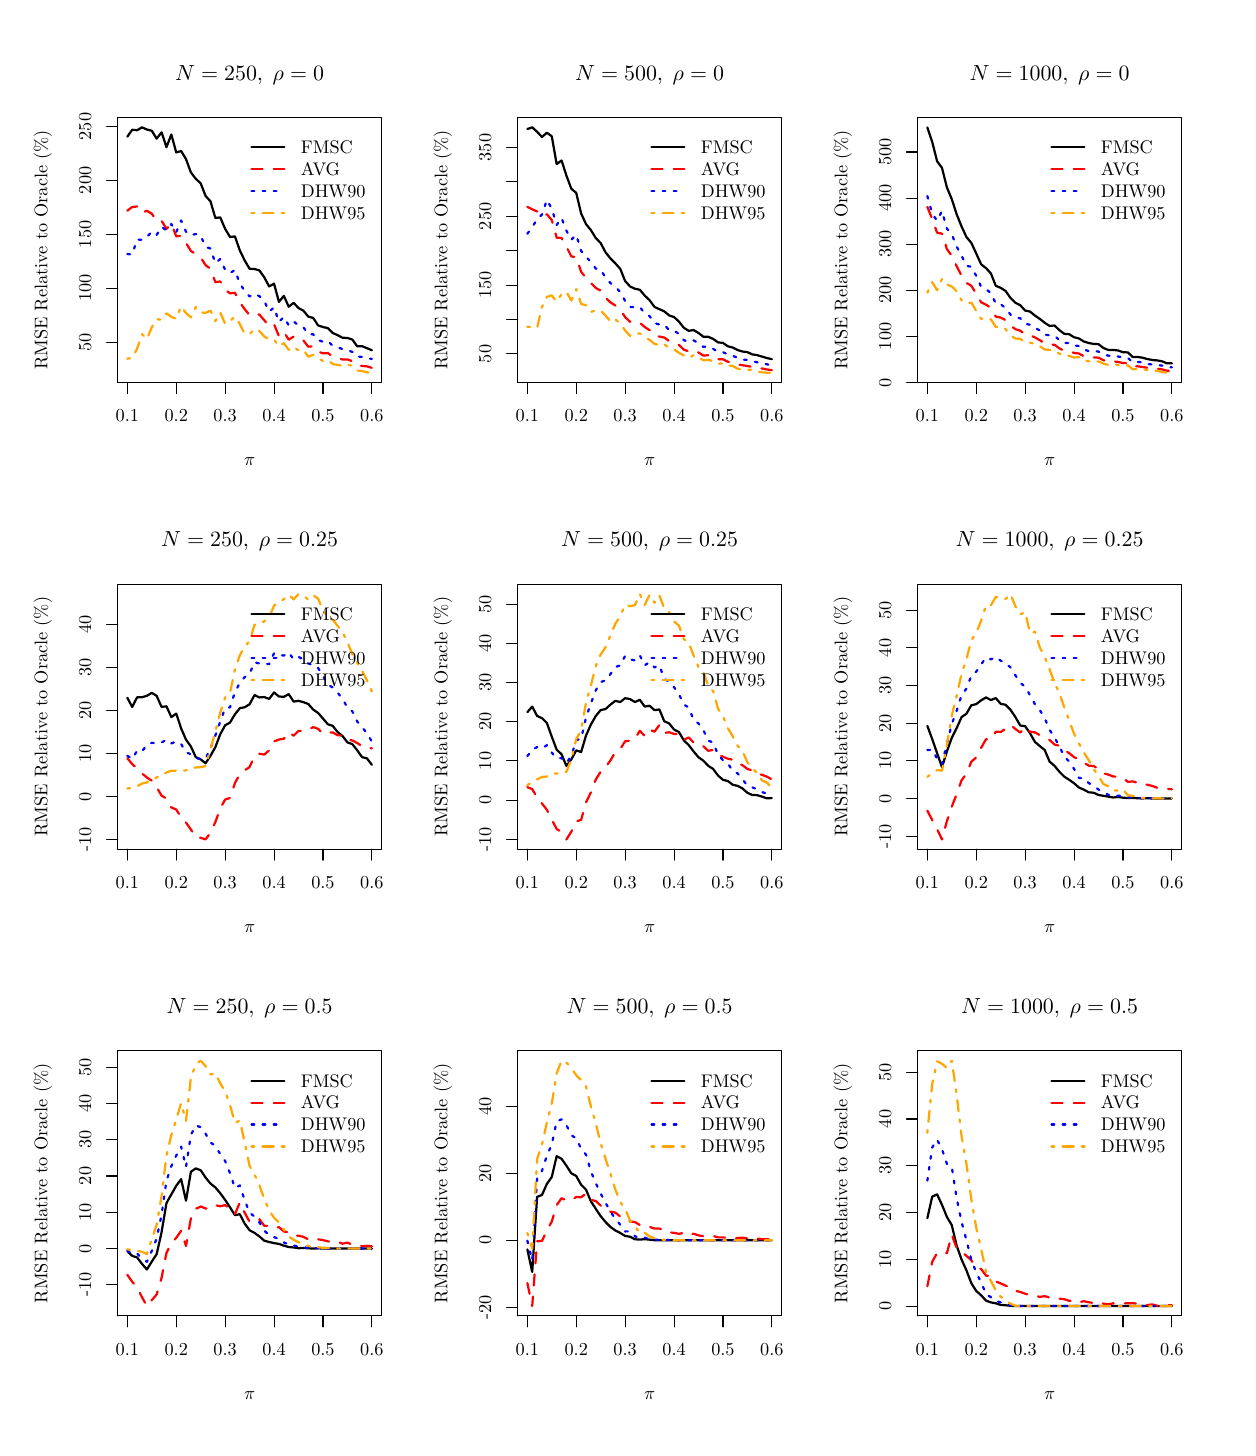
\begin{tikzpicture}[x=1pt,y=1pt]
\definecolor[named]{fillColor}{rgb}{1.00,1.00,1.00}
\path[use as bounding box,fill=fillColor,fill opacity=0.00] (0,0) rectangle (433.62,505.89);
\begin{scope}
\path[clip] ( 32.47,377.65) rectangle (127.91,473.42);
\definecolor[named]{drawColor}{rgb}{0.00,0.00,0.00}

\path[draw=drawColor,line width= 0.8pt,line join=round,line cap=round] ( 36.01,466.50) --
	( 37.77,468.99) --
	( 39.54,468.82) --
	( 41.31,469.87) --
	( 43.08,469.08) --
	( 44.84,468.64) --
	( 46.61,465.78) --
	( 48.38,468.06) --
	( 50.15,462.70) --
	( 51.91,467.27) --
	( 53.68,460.80) --
	( 55.45,461.32) --
	( 57.21,458.40) --
	( 58.98,453.57) --
	( 60.75,451.28) --
	( 62.52,449.63) --
	( 64.28,445.08) --
	( 66.05,443.15) --
	( 67.82,437.11) --
	( 69.59,437.33) --
	( 71.35,433.20) --
	( 73.12,430.23) --
	( 74.89,430.46) --
	( 76.66,425.40) --
	( 78.42,421.75) --
	( 80.19,418.76) --
	( 81.96,418.68) --
	( 83.72,418.17) --
	( 85.49,415.69) --
	( 87.26,412.38) --
	( 89.03,413.37) --
	( 90.79,406.80) --
	( 92.56,408.97) --
	( 94.33,405.06) --
	( 96.10,406.45) --
	( 97.86,404.57) --
	( 99.63,403.63) --
	(101.40,401.48) --
	(103.17,401.00) --
	(104.93,398.30) --
	(106.70,397.70) --
	(108.47,397.32) --
	(110.23,395.57) --
	(112.00,394.75) --
	(113.77,393.83) --
	(115.54,393.77) --
	(117.30,393.19) --
	(119.07,390.74) --
	(120.84,390.78) --
	(122.61,390.08) --
	(124.37,389.32);
\end{scope}
\begin{scope}
\path[clip] (  0.00,  0.00) rectangle (433.62,505.89);
\definecolor[named]{drawColor}{rgb}{0.00,0.00,0.00}

\path[draw=drawColor,line width= 0.4pt,line join=round,line cap=round] ( 36.01,377.65) -- (124.37,377.65);

\path[draw=drawColor,line width= 0.4pt,line join=round,line cap=round] ( 36.01,377.65) -- ( 36.01,373.69);

\path[draw=drawColor,line width= 0.4pt,line join=round,line cap=round] ( 53.68,377.65) -- ( 53.68,373.69);

\path[draw=drawColor,line width= 0.4pt,line join=round,line cap=round] ( 71.35,377.65) -- ( 71.35,373.69);

\path[draw=drawColor,line width= 0.4pt,line join=round,line cap=round] ( 89.03,377.65) -- ( 89.03,373.69);

\path[draw=drawColor,line width= 0.4pt,line join=round,line cap=round] (106.70,377.65) -- (106.70,373.69);

\path[draw=drawColor,line width= 0.4pt,line join=round,line cap=round] (124.37,377.65) -- (124.37,373.69);

\node[text=drawColor,anchor=base,inner sep=0pt, outer sep=0pt, scale=  0.66] at ( 36.01,363.40) {0.1};

\node[text=drawColor,anchor=base,inner sep=0pt, outer sep=0pt, scale=  0.66] at ( 53.68,363.40) {0.2};

\node[text=drawColor,anchor=base,inner sep=0pt, outer sep=0pt, scale=  0.66] at ( 71.35,363.40) {0.3};

\node[text=drawColor,anchor=base,inner sep=0pt, outer sep=0pt, scale=  0.66] at ( 89.03,363.40) {0.4};

\node[text=drawColor,anchor=base,inner sep=0pt, outer sep=0pt, scale=  0.66] at (106.70,363.40) {0.5};

\node[text=drawColor,anchor=base,inner sep=0pt, outer sep=0pt, scale=  0.66] at (124.37,363.40) {0.6};

\path[draw=drawColor,line width= 0.4pt,line join=round,line cap=round] ( 32.47,392.27) -- ( 32.47,470.18);

\path[draw=drawColor,line width= 0.4pt,line join=round,line cap=round] ( 32.47,392.27) -- ( 28.51,392.27);

\path[draw=drawColor,line width= 0.4pt,line join=round,line cap=round] ( 32.47,411.75) -- ( 28.51,411.75);

\path[draw=drawColor,line width= 0.4pt,line join=round,line cap=round] ( 32.47,431.22) -- ( 28.51,431.22);

\path[draw=drawColor,line width= 0.4pt,line join=round,line cap=round] ( 32.47,450.70) -- ( 28.51,450.70);

\path[draw=drawColor,line width= 0.4pt,line join=round,line cap=round] ( 32.47,470.18) -- ( 28.51,470.18);

\node[text=drawColor,rotate= 90.00,anchor=base,inner sep=0pt, outer sep=0pt, scale=  0.66] at ( 22.97,392.27) {50};

\node[text=drawColor,rotate= 90.00,anchor=base,inner sep=0pt, outer sep=0pt, scale=  0.66] at ( 22.97,411.75) {100};

\node[text=drawColor,rotate= 90.00,anchor=base,inner sep=0pt, outer sep=0pt, scale=  0.66] at ( 22.97,431.22) {150};

\node[text=drawColor,rotate= 90.00,anchor=base,inner sep=0pt, outer sep=0pt, scale=  0.66] at ( 22.97,450.70) {200};

\node[text=drawColor,rotate= 90.00,anchor=base,inner sep=0pt, outer sep=0pt, scale=  0.66] at ( 22.97,470.18) {250};

\path[draw=drawColor,line width= 0.4pt,line join=round,line cap=round] ( 32.47,377.65) --
	(127.91,377.65) --
	(127.91,473.42) --
	( 32.47,473.42) --
	( 32.47,377.65);
\end{scope}
\begin{scope}
\path[clip] (  0.00,337.26) rectangle (144.54,505.89);
\definecolor[named]{drawColor}{rgb}{0.00,0.00,0.00}

\node[text=drawColor,anchor=base,inner sep=0pt, outer sep=0pt, scale=  0.79] at ( 80.19,486.92) {\bfseries $N=250, \;\rho=0$};

\node[text=drawColor,anchor=base,inner sep=0pt, outer sep=0pt, scale=  0.66] at ( 80.19,347.56) {$\pi$};

\node[text=drawColor,rotate= 90.00,anchor=base,inner sep=0pt, outer sep=0pt, scale=  0.66] at (  7.13,425.53) {RMSE Relative to Oracle (\%)};
\end{scope}
\begin{scope}
\path[clip] ( 32.47,377.65) rectangle (127.91,473.42);
\definecolor[named]{drawColor}{rgb}{1.00,0.00,0.00}

\path[draw=drawColor,line width= 0.8pt,dash pattern=on 4pt off 4pt ,line join=round,line cap=round] ( 36.01,439.75) --
	( 37.77,441.08) --
	( 39.54,441.26) --
	( 41.31,438.95) --
	( 43.08,439.73) --
	( 44.84,438.67) --
	( 46.61,436.11) --
	( 48.38,436.12) --
	( 50.15,433.20) --
	( 51.91,435.03) --
	( 53.68,430.50) --
	( 55.45,430.65) --
	( 57.21,428.10) --
	( 58.98,425.19) --
	( 60.75,424.09) --
	( 62.52,422.87) --
	( 64.28,420.09) --
	( 66.05,418.71) --
	( 67.82,413.92) --
	( 69.59,414.19) --
	( 71.35,411.25) --
	( 73.12,409.87) --
	( 74.89,410.10) --
	( 76.66,406.66) --
	( 78.42,404.15) --
	( 80.19,402.03) --
	( 81.96,402.55) --
	( 83.72,402.21) --
	( 85.49,400.17) --
	( 87.26,397.99) --
	( 89.03,398.66) --
	( 90.79,394.43) --
	( 92.56,395.95) --
	( 94.33,393.14) --
	( 96.10,394.26) --
	( 97.86,393.05) --
	( 99.63,392.85) --
	(101.40,390.61) --
	(103.17,390.72) --
	(104.93,388.83) --
	(106.70,388.24) --
	(108.47,388.30) --
	(110.23,387.06) --
	(112.00,386.60) --
	(113.77,385.95) --
	(115.54,386.02) --
	(117.30,385.34) --
	(119.07,383.90) --
	(120.84,383.66) --
	(122.61,383.50) --
	(124.37,382.96);
\definecolor[named]{drawColor}{rgb}{0.00,0.00,1.00}

\path[draw=drawColor,line width= 0.8pt,dash pattern=on 1pt off 3pt ,line join=round,line cap=round] ( 36.01,424.09) --
	( 37.77,423.93) --
	( 39.54,429.35) --
	( 41.31,429.20) --
	( 43.08,430.23) --
	( 44.84,432.19) --
	( 46.61,431.03) --
	( 48.38,433.85) --
	( 50.15,432.69) --
	( 51.91,434.93) --
	( 53.68,431.95) --
	( 55.45,436.20) --
	( 57.21,432.17) --
	( 58.98,430.86) --
	( 60.75,431.32) --
	( 62.52,430.75) --
	( 64.28,426.63) --
	( 66.05,426.09) --
	( 67.82,420.75) --
	( 69.59,422.28) --
	( 71.35,418.38) --
	( 73.12,417.19) --
	( 74.89,418.35) --
	( 76.66,413.39) --
	( 78.42,410.81) --
	( 80.19,408.76) --
	( 81.96,409.68) --
	( 83.72,408.87) --
	( 85.49,407.10) --
	( 87.26,403.28) --
	( 89.03,404.82) --
	( 90.79,399.52) --
	( 92.56,401.38) --
	( 94.33,398.33) --
	( 96.10,399.79) --
	( 97.86,398.20) --
	( 99.63,397.63) --
	(101.40,395.14) --
	(103.17,395.09) --
	(104.93,393.03) --
	(106.70,392.37) --
	(108.47,392.61) --
	(110.23,390.94) --
	(112.00,390.32) --
	(113.77,389.76) --
	(115.54,389.41) --
	(117.30,388.71) --
	(119.07,387.04) --
	(120.84,386.90) --
	(122.61,386.52) --
	(124.37,386.17);
\definecolor[named]{drawColor}{rgb}{1.00,0.65,0.00}

\path[draw=drawColor,line width= 0.8pt,dash pattern=on 1pt off 3pt on 4pt off 3pt ,line join=round,line cap=round] ( 36.01,386.26) --
	( 37.77,386.55) --
	( 39.54,389.89) --
	( 41.31,395.15) --
	( 43.08,393.36) --
	( 44.84,397.60) --
	( 46.61,400.55) --
	( 48.38,400.34) --
	( 50.15,402.66) --
	( 51.91,401.39) --
	( 53.68,400.69) --
	( 55.45,405.20) --
	( 57.21,402.74) --
	( 58.98,401.21) --
	( 60.75,404.93) --
	( 62.52,403.02) --
	( 64.28,402.82) --
	( 66.05,403.64) --
	( 67.82,399.88) --
	( 69.59,402.98) --
	( 71.35,398.87) --
	( 73.12,399.89) --
	( 74.89,401.49) --
	( 76.66,398.81) --
	( 78.42,395.31) --
	( 80.19,395.15) --
	( 81.96,397.07) --
	( 83.72,396.22) --
	( 85.49,394.29) --
	( 87.26,393.28) --
	( 89.03,393.10) --
	( 90.79,390.73) --
	( 92.56,391.93) --
	( 94.33,389.46) --
	( 96.10,390.62) --
	( 97.86,389.21) --
	( 99.63,389.44) --
	(101.40,386.97) --
	(103.17,387.66) --
	(104.93,386.46) --
	(106.70,385.45) --
	(108.47,385.79) --
	(110.23,384.32) --
	(112.00,384.06) --
	(113.77,383.68) --
	(115.54,384.25) --
	(117.30,383.63) --
	(119.07,382.00) --
	(120.84,381.80) --
	(122.61,381.34) --
	(124.37,381.20);
\definecolor[named]{drawColor}{rgb}{0.00,0.00,0.00}

\path[draw=drawColor,line width= 0.8pt,line join=round,line cap=round] ( 80.89,462.63) -- ( 92.77,462.63);
\definecolor[named]{drawColor}{rgb}{1.00,0.00,0.00}

\path[draw=drawColor,line width= 0.8pt,dash pattern=on 4pt off 4pt ,line join=round,line cap=round] ( 80.89,454.71) -- ( 92.77,454.71);
\definecolor[named]{drawColor}{rgb}{0.00,0.00,1.00}

\path[draw=drawColor,line width= 0.8pt,dash pattern=on 1pt off 3pt ,line join=round,line cap=round] ( 80.89,446.79) -- ( 92.77,446.79);
\definecolor[named]{drawColor}{rgb}{1.00,0.65,0.00}

\path[draw=drawColor,line width= 0.8pt,dash pattern=on 1pt off 3pt on 4pt off 3pt ,line join=round,line cap=round] ( 80.89,438.87) -- ( 92.77,438.87);
\definecolor[named]{drawColor}{rgb}{0.00,0.00,0.00}

\node[text=drawColor,anchor=base west,inner sep=0pt, outer sep=0pt, scale=  0.66] at ( 98.71,460.35) {FMSC};

\node[text=drawColor,anchor=base west,inner sep=0pt, outer sep=0pt, scale=  0.66] at ( 98.71,452.43) {AVG};

\node[text=drawColor,anchor=base west,inner sep=0pt, outer sep=0pt, scale=  0.66] at ( 98.71,444.51) {DHW90};

\node[text=drawColor,anchor=base west,inner sep=0pt, outer sep=0pt, scale=  0.66] at ( 98.71,436.59) {DHW95};
\end{scope}
\begin{scope}
\path[clip] (177.01,377.65) rectangle (272.45,473.42);
\definecolor[named]{drawColor}{rgb}{0.00,0.00,0.00}

\path[draw=drawColor,line width= 0.8pt,line join=round,line cap=round] (180.55,469.26) --
	(182.31,469.87) --
	(184.08,468.27) --
	(185.85,466.38) --
	(187.62,467.93) --
	(189.38,466.64) --
	(191.15,456.59) --
	(192.92,457.89) --
	(194.69,452.39) --
	(196.45,447.68) --
	(198.22,446.19) --
	(199.99,438.74) --
	(201.75,434.90) --
	(203.52,432.73) --
	(205.29,429.86) --
	(207.06,428.05) --
	(208.82,424.69) --
	(210.59,422.49) --
	(212.36,420.71) --
	(214.13,418.72) --
	(215.89,414.33) --
	(217.66,412.37) --
	(219.43,411.55) --
	(221.20,411.18) --
	(222.96,409.08) --
	(224.73,407.39) --
	(226.50,404.97) --
	(228.26,404.17) --
	(230.03,403.37) --
	(231.80,401.90) --
	(233.57,401.31) --
	(235.33,399.68) --
	(237.10,397.44) --
	(238.87,396.33) --
	(240.64,396.62) --
	(242.40,395.57) --
	(244.17,394.18) --
	(245.94,394.18) --
	(247.71,393.41) --
	(249.47,392.16) --
	(251.24,391.97) --
	(253.01,390.75) --
	(254.77,390.31) --
	(256.54,389.39) --
	(258.31,388.86) --
	(260.08,388.63) --
	(261.84,387.82) --
	(263.61,387.56) --
	(265.38,387.02) --
	(267.15,386.50) --
	(268.91,386.10);
\end{scope}
\begin{scope}
\path[clip] (  0.00,  0.00) rectangle (433.62,505.89);
\definecolor[named]{drawColor}{rgb}{0.00,0.00,0.00}

\path[draw=drawColor,line width= 0.4pt,line join=round,line cap=round] (180.55,377.65) -- (268.91,377.65);

\path[draw=drawColor,line width= 0.4pt,line join=round,line cap=round] (180.55,377.65) -- (180.55,373.69);

\path[draw=drawColor,line width= 0.4pt,line join=round,line cap=round] (198.22,377.65) -- (198.22,373.69);

\path[draw=drawColor,line width= 0.4pt,line join=round,line cap=round] (215.89,377.65) -- (215.89,373.69);

\path[draw=drawColor,line width= 0.4pt,line join=round,line cap=round] (233.57,377.65) -- (233.57,373.69);

\path[draw=drawColor,line width= 0.4pt,line join=round,line cap=round] (251.24,377.65) -- (251.24,373.69);

\path[draw=drawColor,line width= 0.4pt,line join=round,line cap=round] (268.91,377.65) -- (268.91,373.69);

\node[text=drawColor,anchor=base,inner sep=0pt, outer sep=0pt, scale=  0.66] at (180.55,363.40) {0.1};

\node[text=drawColor,anchor=base,inner sep=0pt, outer sep=0pt, scale=  0.66] at (198.22,363.40) {0.2};

\node[text=drawColor,anchor=base,inner sep=0pt, outer sep=0pt, scale=  0.66] at (215.89,363.40) {0.3};

\node[text=drawColor,anchor=base,inner sep=0pt, outer sep=0pt, scale=  0.66] at (233.57,363.40) {0.4};

\node[text=drawColor,anchor=base,inner sep=0pt, outer sep=0pt, scale=  0.66] at (251.24,363.40) {0.5};

\node[text=drawColor,anchor=base,inner sep=0pt, outer sep=0pt, scale=  0.66] at (268.91,363.40) {0.6};

\path[draw=drawColor,line width= 0.4pt,line join=round,line cap=round] (177.01,388.00) -- (177.01,462.59);

\path[draw=drawColor,line width= 0.4pt,line join=round,line cap=round] (177.01,388.00) -- (173.05,388.00);

\path[draw=drawColor,line width= 0.4pt,line join=round,line cap=round] (177.01,400.43) -- (173.05,400.43);

\path[draw=drawColor,line width= 0.4pt,line join=round,line cap=round] (177.01,412.86) -- (173.05,412.86);

\path[draw=drawColor,line width= 0.4pt,line join=round,line cap=round] (177.01,425.29) -- (173.05,425.29);

\path[draw=drawColor,line width= 0.4pt,line join=round,line cap=round] (177.01,437.72) -- (173.05,437.72);

\path[draw=drawColor,line width= 0.4pt,line join=round,line cap=round] (177.01,450.15) -- (173.05,450.15);

\path[draw=drawColor,line width= 0.4pt,line join=round,line cap=round] (177.01,462.59) -- (173.05,462.59);

\node[text=drawColor,rotate= 90.00,anchor=base,inner sep=0pt, outer sep=0pt, scale=  0.66] at (167.51,388.00) {50};

\node[text=drawColor,rotate= 90.00,anchor=base,inner sep=0pt, outer sep=0pt, scale=  0.66] at (167.51,412.86) {150};

\node[text=drawColor,rotate= 90.00,anchor=base,inner sep=0pt, outer sep=0pt, scale=  0.66] at (167.51,437.72) {250};

\node[text=drawColor,rotate= 90.00,anchor=base,inner sep=0pt, outer sep=0pt, scale=  0.66] at (167.51,462.59) {350};

\path[draw=drawColor,line width= 0.4pt,line join=round,line cap=round] (177.01,377.65) --
	(272.45,377.65) --
	(272.45,473.42) --
	(177.01,473.42) --
	(177.01,377.65);
\end{scope}
\begin{scope}
\path[clip] (144.54,337.26) rectangle (289.08,505.89);
\definecolor[named]{drawColor}{rgb}{0.00,0.00,0.00}

\node[text=drawColor,anchor=base,inner sep=0pt, outer sep=0pt, scale=  0.79] at (224.73,486.92) {\bfseries $N=500, \;\rho=0$};

\node[text=drawColor,anchor=base,inner sep=0pt, outer sep=0pt, scale=  0.66] at (224.73,347.56) {$\pi$};

\node[text=drawColor,rotate= 90.00,anchor=base,inner sep=0pt, outer sep=0pt, scale=  0.66] at (151.67,425.53) {RMSE Relative to Oracle (\%)};
\end{scope}
\begin{scope}
\path[clip] (177.01,377.65) rectangle (272.45,473.42);
\definecolor[named]{drawColor}{rgb}{1.00,0.00,0.00}

\path[draw=drawColor,line width= 0.8pt,dash pattern=on 4pt off 4pt ,line join=round,line cap=round] (180.55,441.15) --
	(182.31,440.25) --
	(184.08,439.46) --
	(185.85,437.75) --
	(187.62,438.44) --
	(189.38,436.36) --
	(191.15,429.99) --
	(192.92,429.90) --
	(194.69,426.75) --
	(196.45,423.22) --
	(198.22,422.96) --
	(199.99,417.69) --
	(201.75,415.42) --
	(203.52,413.60) --
	(205.29,411.82) --
	(207.06,410.88) --
	(208.82,408.28) --
	(210.59,406.61) --
	(212.36,405.50) --
	(214.13,404.12) --
	(215.89,401.28) --
	(217.66,399.61) --
	(219.43,399.39) --
	(221.20,399.25) --
	(222.96,397.72) --
	(224.73,396.58) --
	(226.50,394.74) --
	(228.26,394.27) --
	(230.03,393.92) --
	(231.80,392.63) --
	(233.57,392.33) --
	(235.33,391.23) --
	(237.10,389.55) --
	(238.87,388.90) --
	(240.64,389.21) --
	(242.40,388.52) --
	(244.17,387.38) --
	(245.94,387.54) --
	(247.71,387.00) --
	(249.47,386.08) --
	(251.24,386.05) --
	(253.01,385.18) --
	(254.77,384.81) --
	(256.54,384.26) --
	(258.31,383.89) --
	(260.08,383.64) --
	(261.84,383.25) --
	(263.61,382.97) --
	(265.38,382.73) --
	(267.15,382.37) --
	(268.91,382.16);
\definecolor[named]{drawColor}{rgb}{0.00,0.00,1.00}

\path[draw=drawColor,line width= 0.8pt,dash pattern=on 1pt off 3pt ,line join=round,line cap=round] (180.55,431.40) --
	(182.31,433.79) --
	(184.08,436.64) --
	(185.85,438.38) --
	(187.62,443.64) --
	(189.38,440.50) --
	(191.15,434.60) --
	(192.92,437.13) --
	(194.69,432.50) --
	(196.45,429.26) --
	(198.22,431.04) --
	(199.99,425.19) --
	(201.75,423.11) --
	(203.52,421.22) --
	(205.29,418.82) --
	(207.06,418.44) --
	(208.82,415.55) --
	(210.59,413.60) --
	(212.36,412.20) --
	(214.13,410.34) --
	(215.89,407.14) --
	(217.66,405.01) --
	(219.43,404.83) --
	(221.20,404.91) --
	(222.96,402.71) --
	(224.73,401.65) --
	(226.50,399.10) --
	(228.26,398.66) --
	(230.03,398.47) --
	(231.80,396.61) --
	(233.57,396.41) --
	(235.33,395.24) --
	(237.10,392.97) --
	(238.87,392.31) --
	(240.64,392.89) --
	(242.40,391.90) --
	(244.17,390.54) --
	(245.94,390.64) --
	(247.71,389.81) --
	(249.47,388.69) --
	(251.24,388.63) --
	(253.01,387.83) --
	(254.77,387.32) --
	(256.54,386.58) --
	(258.31,385.95) --
	(260.08,385.83) --
	(261.84,385.39) --
	(263.61,384.94) --
	(265.38,384.72) --
	(267.15,384.25) --
	(268.91,383.77);
\definecolor[named]{drawColor}{rgb}{1.00,0.65,0.00}

\path[draw=drawColor,line width= 0.8pt,dash pattern=on 1pt off 3pt on 4pt off 3pt ,line join=round,line cap=round] (180.55,397.83) --
	(182.31,397.61) --
	(184.08,397.41) --
	(185.85,405.02) --
	(187.62,408.59) --
	(189.38,409.15) --
	(191.15,406.87) --
	(192.92,409.65) --
	(194.69,410.41) --
	(196.45,407.29) --
	(198.22,411.43) --
	(199.99,406.05) --
	(201.75,405.56) --
	(203.52,403.20) --
	(205.29,403.66) --
	(207.06,403.67) --
	(208.82,401.83) --
	(210.59,399.70) --
	(212.36,400.54) --
	(214.13,398.95) --
	(215.89,396.50) --
	(217.66,394.49) --
	(219.43,395.46) --
	(221.20,395.36) --
	(222.96,394.20) --
	(224.73,393.04) --
	(226.50,391.64) --
	(228.26,391.18) --
	(230.03,391.52) --
	(231.80,390.01) --
	(233.57,389.65) --
	(235.33,388.38) --
	(237.10,387.44) --
	(238.87,386.52) --
	(240.64,387.55) --
	(242.40,386.84) --
	(244.17,385.68) --
	(245.94,385.82) --
	(247.71,385.39) --
	(249.47,384.45) --
	(251.24,384.57) --
	(253.01,383.88) --
	(254.77,383.65) --
	(256.54,382.65) --
	(258.31,382.43) --
	(260.08,382.29) --
	(261.84,382.25) --
	(263.61,381.55) --
	(265.38,381.35) --
	(267.15,381.20) --
	(268.91,381.20);
\definecolor[named]{drawColor}{rgb}{0.00,0.00,0.00}

\path[draw=drawColor,line width= 0.8pt,line join=round,line cap=round] (225.43,462.63) -- (237.31,462.63);
\definecolor[named]{drawColor}{rgb}{1.00,0.00,0.00}

\path[draw=drawColor,line width= 0.8pt,dash pattern=on 4pt off 4pt ,line join=round,line cap=round] (225.43,454.71) -- (237.31,454.71);
\definecolor[named]{drawColor}{rgb}{0.00,0.00,1.00}

\path[draw=drawColor,line width= 0.8pt,dash pattern=on 1pt off 3pt ,line join=round,line cap=round] (225.43,446.79) -- (237.31,446.79);
\definecolor[named]{drawColor}{rgb}{1.00,0.65,0.00}

\path[draw=drawColor,line width= 0.8pt,dash pattern=on 1pt off 3pt on 4pt off 3pt ,line join=round,line cap=round] (225.43,438.87) -- (237.31,438.87);
\definecolor[named]{drawColor}{rgb}{0.00,0.00,0.00}

\node[text=drawColor,anchor=base west,inner sep=0pt, outer sep=0pt, scale=  0.66] at (243.25,460.35) {FMSC};

\node[text=drawColor,anchor=base west,inner sep=0pt, outer sep=0pt, scale=  0.66] at (243.25,452.43) {AVG};

\node[text=drawColor,anchor=base west,inner sep=0pt, outer sep=0pt, scale=  0.66] at (243.25,444.51) {DHW90};

\node[text=drawColor,anchor=base west,inner sep=0pt, outer sep=0pt, scale=  0.66] at (243.25,436.59) {DHW95};
\end{scope}
\begin{scope}
\path[clip] (321.55,377.65) rectangle (416.99,473.42);
\definecolor[named]{drawColor}{rgb}{0.00,0.00,0.00}

\path[draw=drawColor,line width= 0.8pt,line join=round,line cap=round] (325.09,469.87) --
	(326.85,464.60) --
	(328.62,457.60) --
	(330.39,455.22) --
	(332.16,448.15) --
	(333.92,443.94) --
	(335.69,438.44) --
	(337.46,434.05) --
	(339.23,430.21) --
	(340.99,428.11) --
	(342.76,424.28) --
	(344.53,420.37) --
	(346.29,419.00) --
	(348.06,417.07) --
	(349.83,412.59) --
	(351.60,411.87) --
	(353.36,410.75) --
	(355.13,408.24) --
	(356.90,406.48) --
	(358.67,405.60) --
	(360.43,403.66) --
	(362.20,403.30) --
	(363.97,401.85) --
	(365.74,400.64) --
	(367.50,399.26) --
	(369.27,398.10) --
	(371.04,398.26) --
	(372.80,396.60) --
	(374.57,395.26) --
	(376.34,395.11) --
	(378.11,394.02) --
	(379.87,393.58) --
	(381.64,392.48) --
	(383.41,391.94) --
	(385.18,391.61) --
	(386.94,391.52) --
	(388.71,390.14) --
	(390.48,389.42) --
	(392.25,389.45) --
	(394.01,389.24) --
	(395.78,388.61) --
	(397.55,388.54) --
	(399.31,386.88) --
	(401.08,386.89) --
	(402.85,386.63) --
	(404.62,386.13) --
	(406.38,385.81) --
	(408.15,385.65) --
	(409.92,385.32) --
	(411.69,384.60) --
	(413.45,384.60);
\end{scope}
\begin{scope}
\path[clip] (  0.00,  0.00) rectangle (433.62,505.89);
\definecolor[named]{drawColor}{rgb}{0.00,0.00,0.00}

\path[draw=drawColor,line width= 0.4pt,line join=round,line cap=round] (325.09,377.65) -- (413.45,377.65);

\path[draw=drawColor,line width= 0.4pt,line join=round,line cap=round] (325.09,377.65) -- (325.09,373.69);

\path[draw=drawColor,line width= 0.4pt,line join=round,line cap=round] (342.76,377.65) -- (342.76,373.69);

\path[draw=drawColor,line width= 0.4pt,line join=round,line cap=round] (360.43,377.65) -- (360.43,373.69);

\path[draw=drawColor,line width= 0.4pt,line join=round,line cap=round] (378.11,377.65) -- (378.11,373.69);

\path[draw=drawColor,line width= 0.4pt,line join=round,line cap=round] (395.78,377.65) -- (395.78,373.69);

\path[draw=drawColor,line width= 0.4pt,line join=round,line cap=round] (413.45,377.65) -- (413.45,373.69);

\node[text=drawColor,anchor=base,inner sep=0pt, outer sep=0pt, scale=  0.66] at (325.09,363.40) {0.1};

\node[text=drawColor,anchor=base,inner sep=0pt, outer sep=0pt, scale=  0.66] at (342.76,363.40) {0.2};

\node[text=drawColor,anchor=base,inner sep=0pt, outer sep=0pt, scale=  0.66] at (360.43,363.40) {0.3};

\node[text=drawColor,anchor=base,inner sep=0pt, outer sep=0pt, scale=  0.66] at (378.11,363.40) {0.4};

\node[text=drawColor,anchor=base,inner sep=0pt, outer sep=0pt, scale=  0.66] at (395.78,363.40) {0.5};

\node[text=drawColor,anchor=base,inner sep=0pt, outer sep=0pt, scale=  0.66] at (413.45,363.40) {0.6};

\path[draw=drawColor,line width= 0.4pt,line join=round,line cap=round] (321.55,377.68) -- (321.55,460.95);

\path[draw=drawColor,line width= 0.4pt,line join=round,line cap=round] (321.55,377.68) -- (317.59,377.68);

\path[draw=drawColor,line width= 0.4pt,line join=round,line cap=round] (321.55,394.34) -- (317.59,394.34);

\path[draw=drawColor,line width= 0.4pt,line join=round,line cap=round] (321.55,410.99) -- (317.59,410.99);

\path[draw=drawColor,line width= 0.4pt,line join=round,line cap=round] (321.55,427.64) -- (317.59,427.64);

\path[draw=drawColor,line width= 0.4pt,line join=round,line cap=round] (321.55,444.30) -- (317.59,444.30);

\path[draw=drawColor,line width= 0.4pt,line join=round,line cap=round] (321.55,460.95) -- (317.59,460.95);

\node[text=drawColor,rotate= 90.00,anchor=base,inner sep=0pt, outer sep=0pt, scale=  0.66] at (312.05,377.68) {0};

\node[text=drawColor,rotate= 90.00,anchor=base,inner sep=0pt, outer sep=0pt, scale=  0.66] at (312.05,394.34) {100};

\node[text=drawColor,rotate= 90.00,anchor=base,inner sep=0pt, outer sep=0pt, scale=  0.66] at (312.05,410.99) {200};

\node[text=drawColor,rotate= 90.00,anchor=base,inner sep=0pt, outer sep=0pt, scale=  0.66] at (312.05,427.64) {300};

\node[text=drawColor,rotate= 90.00,anchor=base,inner sep=0pt, outer sep=0pt, scale=  0.66] at (312.05,444.30) {400};

\node[text=drawColor,rotate= 90.00,anchor=base,inner sep=0pt, outer sep=0pt, scale=  0.66] at (312.05,460.95) {500};

\path[draw=drawColor,line width= 0.4pt,line join=round,line cap=round] (321.55,377.65) --
	(416.99,377.65) --
	(416.99,473.42) --
	(321.55,473.42) --
	(321.55,377.65);
\end{scope}
\begin{scope}
\path[clip] (289.08,337.26) rectangle (433.62,505.89);
\definecolor[named]{drawColor}{rgb}{0.00,0.00,0.00}

\node[text=drawColor,anchor=base,inner sep=0pt, outer sep=0pt, scale=  0.79] at (369.27,486.92) {\bfseries $N=1000, \;\rho=0$};

\node[text=drawColor,anchor=base,inner sep=0pt, outer sep=0pt, scale=  0.66] at (369.27,347.56) {$\pi$};

\node[text=drawColor,rotate= 90.00,anchor=base,inner sep=0pt, outer sep=0pt, scale=  0.66] at (296.21,425.53) {RMSE Relative to Oracle (\%)};
\end{scope}
\begin{scope}
\path[clip] (321.55,377.65) rectangle (416.99,473.42);
\definecolor[named]{drawColor}{rgb}{1.00,0.00,0.00}

\path[draw=drawColor,line width= 0.8pt,dash pattern=on 4pt off 4pt ,line join=round,line cap=round] (325.09,441.12) --
	(326.85,436.73) --
	(328.62,431.78) --
	(330.39,431.46) --
	(332.16,425.89) --
	(333.92,423.43) --
	(335.69,419.65) --
	(337.46,416.27) --
	(339.23,413.64) --
	(340.99,412.63) --
	(342.76,409.71) --
	(344.53,406.65) --
	(346.29,405.79) --
	(348.06,404.64) --
	(349.83,401.47) --
	(351.60,401.13) --
	(353.36,400.20) --
	(355.13,398.27) --
	(356.90,396.94) --
	(358.67,396.40) --
	(360.43,394.97) --
	(362.20,394.73) --
	(363.97,393.99) --
	(365.74,392.95) --
	(367.50,391.83) --
	(369.27,391.33) --
	(371.04,391.33) --
	(372.80,390.00) --
	(374.57,389.13) --
	(376.34,389.03) --
	(378.11,388.35) --
	(379.87,388.14) --
	(381.64,387.15) --
	(383.41,386.80) --
	(385.18,386.74) --
	(386.94,386.63) --
	(388.71,385.72) --
	(390.48,385.20) --
	(392.25,385.31) --
	(394.01,385.10) --
	(395.78,384.69) --
	(397.55,384.65) --
	(399.31,383.45) --
	(401.08,383.52) --
	(402.85,383.27) --
	(404.62,382.98) --
	(406.38,382.66) --
	(408.15,382.64) --
	(409.92,382.41) --
	(411.69,381.91) --
	(413.45,381.90);
\definecolor[named]{drawColor}{rgb}{0.00,0.00,1.00}

\path[draw=drawColor,line width= 0.8pt,dash pattern=on 1pt off 3pt ,line join=round,line cap=round] (325.09,445.06) --
	(326.85,438.61) --
	(328.62,436.14) --
	(330.39,439.65) --
	(332.16,433.28) --
	(333.92,431.24) --
	(335.69,426.73) --
	(337.46,423.51) --
	(339.23,419.85) --
	(340.99,419.45) --
	(342.76,416.21) --
	(344.53,412.24) --
	(346.29,411.39) --
	(348.06,410.00) --
	(349.83,406.15) --
	(351.60,405.94) --
	(353.36,404.56) --
	(355.13,402.20) --
	(356.90,401.15) --
	(358.67,400.88) --
	(360.43,398.89) --
	(362.20,398.53) --
	(363.97,397.39) --
	(365.74,396.48) --
	(367.50,394.94) --
	(369.27,394.74) --
	(371.04,394.60) --
	(372.80,392.97) --
	(374.57,391.94) --
	(376.34,391.97) --
	(378.11,391.03) --
	(379.87,390.86) --
	(381.64,389.57) --
	(383.41,389.03) --
	(385.18,389.11) --
	(386.94,388.83) --
	(388.71,387.76) --
	(390.48,387.39) --
	(392.25,387.08) --
	(394.01,387.07) --
	(395.78,386.69) --
	(397.55,386.57) --
	(399.31,384.92) --
	(401.08,385.12) --
	(402.85,384.94) --
	(404.62,384.33) --
	(406.38,384.18) --
	(408.15,384.05) --
	(409.92,383.76) --
	(411.69,383.17) --
	(413.45,383.15);
\definecolor[named]{drawColor}{rgb}{1.00,0.65,0.00}

\path[draw=drawColor,line width= 0.8pt,dash pattern=on 1pt off 3pt on 4pt off 3pt ,line join=round,line cap=round] (325.09,410.11) --
	(326.85,413.91) --
	(328.62,411.02) --
	(330.39,415.12) --
	(332.16,413.04) --
	(333.92,412.37) --
	(335.69,410.63) --
	(337.46,407.36) --
	(339.23,406.23) --
	(340.99,406.55) --
	(342.76,403.54) --
	(344.53,400.66) --
	(346.29,400.87) --
	(348.06,400.48) --
	(349.83,397.72) --
	(351.60,397.84) --
	(353.36,396.93) --
	(355.13,394.72) --
	(356.90,393.53) --
	(358.67,393.49) --
	(360.43,392.04) --
	(362.20,392.01) --
	(363.97,391.65) --
	(365.74,390.78) --
	(367.50,389.61) --
	(369.27,389.44) --
	(371.04,389.24) --
	(372.80,388.08) --
	(374.57,387.40) --
	(376.34,387.29) --
	(378.11,386.66) --
	(379.87,386.86) --
	(381.64,385.65) --
	(383.41,385.35) --
	(385.18,385.30) --
	(386.94,385.29) --
	(388.71,384.46) --
	(390.48,384.04) --
	(392.25,384.37) --
	(394.01,384.00) --
	(395.78,383.54) --
	(397.55,383.91) --
	(399.31,382.43) --
	(401.08,382.54) --
	(402.85,382.58) --
	(404.62,382.12) --
	(406.38,381.99) --
	(408.15,381.89) --
	(409.92,381.41) --
	(411.69,381.27) --
	(413.45,381.20);
\definecolor[named]{drawColor}{rgb}{0.00,0.00,0.00}

\path[draw=drawColor,line width= 0.8pt,line join=round,line cap=round] (369.97,462.63) -- (381.85,462.63);
\definecolor[named]{drawColor}{rgb}{1.00,0.00,0.00}

\path[draw=drawColor,line width= 0.8pt,dash pattern=on 4pt off 4pt ,line join=round,line cap=round] (369.97,454.71) -- (381.85,454.71);
\definecolor[named]{drawColor}{rgb}{0.00,0.00,1.00}

\path[draw=drawColor,line width= 0.8pt,dash pattern=on 1pt off 3pt ,line join=round,line cap=round] (369.97,446.79) -- (381.85,446.79);
\definecolor[named]{drawColor}{rgb}{1.00,0.65,0.00}

\path[draw=drawColor,line width= 0.8pt,dash pattern=on 1pt off 3pt on 4pt off 3pt ,line join=round,line cap=round] (369.97,438.87) -- (381.85,438.87);
\definecolor[named]{drawColor}{rgb}{0.00,0.00,0.00}

\node[text=drawColor,anchor=base west,inner sep=0pt, outer sep=0pt, scale=  0.66] at (387.79,460.35) {FMSC};

\node[text=drawColor,anchor=base west,inner sep=0pt, outer sep=0pt, scale=  0.66] at (387.79,452.43) {AVG};

\node[text=drawColor,anchor=base west,inner sep=0pt, outer sep=0pt, scale=  0.66] at (387.79,444.51) {DHW90};

\node[text=drawColor,anchor=base west,inner sep=0pt, outer sep=0pt, scale=  0.66] at (387.79,436.59) {DHW95};
\end{scope}
\begin{scope}
\path[clip] ( 32.47,209.02) rectangle (127.91,304.79);
\definecolor[named]{drawColor}{rgb}{0.00,0.00,0.00}

\path[draw=drawColor,line width= 0.8pt,line join=round,line cap=round] ( 36.01,263.75) --
	( 37.77,260.42) --
	( 39.54,263.91) --
	( 41.31,263.93) --
	( 43.08,264.47) --
	( 44.84,265.52) --
	( 46.61,264.44) --
	( 48.38,260.46) --
	( 50.15,260.66) --
	( 51.91,256.77) --
	( 53.68,258.02) --
	( 55.45,252.68) --
	( 57.21,248.62) --
	( 58.98,246.15) --
	( 60.75,242.29) --
	( 62.52,241.48) --
	( 64.28,240.07) --
	( 66.05,242.77) --
	( 67.82,245.90) --
	( 69.59,250.58) --
	( 71.35,253.79) --
	( 73.12,254.80) --
	( 74.89,257.77) --
	( 76.66,260.00) --
	( 78.42,260.32) --
	( 80.19,261.40) --
	( 81.96,264.73) --
	( 83.72,263.87) --
	( 85.49,264.00) --
	( 87.26,263.33) --
	( 89.03,265.66) --
	( 90.79,264.21) --
	( 92.56,264.08) --
	( 94.33,265.07) --
	( 96.10,262.36) --
	( 97.86,262.65) --
	( 99.63,262.16) --
	(101.40,261.49) --
	(103.17,259.47) --
	(104.93,258.28) --
	(106.70,256.25) --
	(108.47,254.18) --
	(110.23,253.59) --
	(112.00,251.36) --
	(113.77,249.93) --
	(115.54,247.62) --
	(117.30,247.01) --
	(119.07,244.78) --
	(120.84,242.29) --
	(122.61,241.84) --
	(124.37,239.53);
\end{scope}
\begin{scope}
\path[clip] (  0.00,  0.00) rectangle (433.62,505.89);
\definecolor[named]{drawColor}{rgb}{0.00,0.00,0.00}

\path[draw=drawColor,line width= 0.4pt,line join=round,line cap=round] ( 36.01,209.02) -- (124.37,209.02);

\path[draw=drawColor,line width= 0.4pt,line join=round,line cap=round] ( 36.01,209.02) -- ( 36.01,205.06);

\path[draw=drawColor,line width= 0.4pt,line join=round,line cap=round] ( 53.68,209.02) -- ( 53.68,205.06);

\path[draw=drawColor,line width= 0.4pt,line join=round,line cap=round] ( 71.35,209.02) -- ( 71.35,205.06);

\path[draw=drawColor,line width= 0.4pt,line join=round,line cap=round] ( 89.03,209.02) -- ( 89.03,205.06);

\path[draw=drawColor,line width= 0.4pt,line join=round,line cap=round] (106.70,209.02) -- (106.70,205.06);

\path[draw=drawColor,line width= 0.4pt,line join=round,line cap=round] (124.37,209.02) -- (124.37,205.06);

\node[text=drawColor,anchor=base,inner sep=0pt, outer sep=0pt, scale=  0.66] at ( 36.01,194.77) {0.1};

\node[text=drawColor,anchor=base,inner sep=0pt, outer sep=0pt, scale=  0.66] at ( 53.68,194.77) {0.2};

\node[text=drawColor,anchor=base,inner sep=0pt, outer sep=0pt, scale=  0.66] at ( 71.35,194.77) {0.3};

\node[text=drawColor,anchor=base,inner sep=0pt, outer sep=0pt, scale=  0.66] at ( 89.03,194.77) {0.4};

\node[text=drawColor,anchor=base,inner sep=0pt, outer sep=0pt, scale=  0.66] at (106.70,194.77) {0.5};

\node[text=drawColor,anchor=base,inner sep=0pt, outer sep=0pt, scale=  0.66] at (124.37,194.77) {0.6};

\path[draw=drawColor,line width= 0.4pt,line join=round,line cap=round] ( 32.47,212.52) -- ( 32.47,290.24);

\path[draw=drawColor,line width= 0.4pt,line join=round,line cap=round] ( 32.47,212.52) -- ( 28.51,212.52);

\path[draw=drawColor,line width= 0.4pt,line join=round,line cap=round] ( 32.47,228.06) -- ( 28.51,228.06);

\path[draw=drawColor,line width= 0.4pt,line join=round,line cap=round] ( 32.47,243.61) -- ( 28.51,243.61);

\path[draw=drawColor,line width= 0.4pt,line join=round,line cap=round] ( 32.47,259.15) -- ( 28.51,259.15);

\path[draw=drawColor,line width= 0.4pt,line join=round,line cap=round] ( 32.47,274.70) -- ( 28.51,274.70);

\path[draw=drawColor,line width= 0.4pt,line join=round,line cap=round] ( 32.47,290.24) -- ( 28.51,290.24);

\node[text=drawColor,rotate= 90.00,anchor=base,inner sep=0pt, outer sep=0pt, scale=  0.66] at ( 22.97,212.52) {-10};

\node[text=drawColor,rotate= 90.00,anchor=base,inner sep=0pt, outer sep=0pt, scale=  0.66] at ( 22.97,228.06) {0};

\node[text=drawColor,rotate= 90.00,anchor=base,inner sep=0pt, outer sep=0pt, scale=  0.66] at ( 22.97,243.61) {10};

\node[text=drawColor,rotate= 90.00,anchor=base,inner sep=0pt, outer sep=0pt, scale=  0.66] at ( 22.97,259.15) {20};

\node[text=drawColor,rotate= 90.00,anchor=base,inner sep=0pt, outer sep=0pt, scale=  0.66] at ( 22.97,274.70) {30};

\node[text=drawColor,rotate= 90.00,anchor=base,inner sep=0pt, outer sep=0pt, scale=  0.66] at ( 22.97,290.24) {40};

\path[draw=drawColor,line width= 0.4pt,line join=round,line cap=round] ( 32.47,209.02) --
	(127.91,209.02) --
	(127.91,304.79) --
	( 32.47,304.79) --
	( 32.47,209.02);
\end{scope}
\begin{scope}
\path[clip] (  0.00,168.63) rectangle (144.54,337.26);
\definecolor[named]{drawColor}{rgb}{0.00,0.00,0.00}

\node[text=drawColor,anchor=base,inner sep=0pt, outer sep=0pt, scale=  0.79] at ( 80.19,318.29) {\bfseries $N=250, \;\rho=0.25$};

\node[text=drawColor,anchor=base,inner sep=0pt, outer sep=0pt, scale=  0.66] at ( 80.19,178.93) {$\pi$};

\node[text=drawColor,rotate= 90.00,anchor=base,inner sep=0pt, outer sep=0pt, scale=  0.66] at (  7.13,256.90) {RMSE Relative to Oracle (\%)};
\end{scope}
\begin{scope}
\path[clip] ( 32.47,209.02) rectangle (127.91,304.79);
\definecolor[named]{drawColor}{rgb}{1.00,0.00,0.00}

\path[draw=drawColor,line width= 0.8pt,dash pattern=on 4pt off 4pt ,line join=round,line cap=round] ( 36.01,241.90) --
	( 37.77,239.77) --
	( 39.54,238.17) --
	( 41.31,236.40) --
	( 43.08,234.95) --
	( 44.84,233.78) --
	( 46.61,231.41) --
	( 48.38,228.41) --
	( 50.15,227.30) --
	( 51.91,224.11) --
	( 53.68,223.38) --
	( 55.45,220.48) --
	( 57.21,218.65) --
	( 58.98,216.15) --
	( 60.75,213.38) --
	( 62.52,213.13) --
	( 64.28,212.57) --
	( 66.05,215.00) --
	( 67.82,218.82) --
	( 69.59,223.83) --
	( 71.35,226.96) --
	( 73.12,227.56) --
	( 74.89,232.93) --
	( 76.66,236.18) --
	( 78.42,237.56) --
	( 80.19,238.70) --
	( 81.96,242.69) --
	( 83.72,243.51) --
	( 85.49,243.22) --
	( 87.26,244.76) --
	( 89.03,247.97) --
	( 90.79,248.66) --
	( 92.56,248.92) --
	( 94.33,251.31) --
	( 96.10,250.03) --
	( 97.86,251.78) --
	( 99.63,251.77) --
	(101.40,252.11) --
	(103.17,253.17) --
	(104.93,252.52) --
	(106.70,250.72) --
	(108.47,251.09) --
	(110.23,251.23) --
	(112.00,250.22) --
	(113.77,250.09) --
	(115.54,248.56) --
	(117.30,248.33) --
	(119.07,247.39) --
	(120.84,246.22) --
	(122.61,246.11) --
	(124.37,245.41);
\definecolor[named]{drawColor}{rgb}{0.00,0.00,1.00}

\path[draw=drawColor,line width= 0.8pt,dash pattern=on 1pt off 3pt ,line join=round,line cap=round] ( 36.01,242.79) --
	( 37.77,241.61) --
	( 39.54,244.62) --
	( 41.31,244.37) --
	( 43.08,246.71) --
	( 44.84,247.47) --
	( 46.61,247.36) --
	( 48.38,247.59) --
	( 50.15,248.58) --
	( 51.91,247.26) --
	( 53.68,247.92) --
	( 55.45,247.02) --
	( 57.21,244.05) --
	( 58.98,243.33) --
	( 60.75,241.93) --
	( 62.52,241.66) --
	( 64.28,241.74) --
	( 66.05,245.55) --
	( 67.82,250.12) --
	( 69.59,255.20) --
	( 71.35,259.95) --
	( 73.12,260.30) --
	( 74.89,265.80) --
	( 76.66,269.12) --
	( 78.42,271.23) --
	( 80.19,272.43) --
	( 81.96,276.59) --
	( 83.72,276.14) --
	( 85.49,276.06) --
	( 87.26,275.93) --
	( 89.03,279.83) --
	( 90.79,279.27) --
	( 92.56,278.98) --
	( 94.33,280.14) --
	( 96.10,277.61) --
	( 97.86,278.51) --
	( 99.63,277.61) --
	(101.40,276.14) --
	(103.17,275.52) --
	(104.93,274.54) --
	(106.70,271.73) --
	(108.47,268.48) --
	(110.23,267.47) --
	(112.00,265.62) --
	(113.77,263.32) --
	(115.54,260.19) --
	(117.30,258.85) --
	(119.07,255.19) --
	(120.84,253.06) --
	(122.61,250.98) --
	(124.37,247.90);
\definecolor[named]{drawColor}{rgb}{1.00,0.65,0.00}

\path[draw=drawColor,line width= 0.8pt,dash pattern=on 1pt off 3pt on 4pt off 3pt ,line join=round,line cap=round] ( 36.01,230.96) --
	( 37.77,231.18) --
	( 39.54,231.75) --
	( 41.31,232.75) --
	( 43.08,233.16) --
	( 44.84,234.47) --
	( 46.61,234.90) --
	( 48.38,236.07) --
	( 50.15,236.74) --
	( 51.91,237.42) --
	( 53.68,237.35) --
	( 55.45,237.37) --
	( 57.21,237.53) --
	( 58.98,238.37) --
	( 60.75,238.53) --
	( 62.52,238.69) --
	( 64.28,239.07) --
	( 66.05,245.29) --
	( 67.82,251.51) --
	( 69.59,258.37) --
	( 71.35,263.87) --
	( 73.12,265.51) --
	( 74.89,274.02) --
	( 76.66,279.08) --
	( 78.42,282.32) --
	( 80.19,284.18) --
	( 81.96,290.11) --
	( 83.72,290.37) --
	( 85.49,291.37) --
	( 87.26,292.85) --
	( 89.03,297.04) --
	( 90.79,298.35) --
	( 92.56,299.36) --
	( 94.33,301.05) --
	( 96.10,299.31) --
	( 97.86,301.24) --
	( 99.63,300.62) --
	(101.40,299.26) --
	(103.17,300.76) --
	(104.93,299.61) --
	(106.70,295.34) --
	(108.47,292.96) --
	(110.23,291.92) --
	(112.00,289.74) --
	(113.77,287.53) --
	(115.54,283.73) --
	(117.30,279.60) --
	(119.07,276.39) --
	(120.84,273.47) --
	(122.61,270.04) --
	(124.37,266.04);
\definecolor[named]{drawColor}{rgb}{0.00,0.00,0.00}

\path[draw=drawColor,line width= 0.8pt,line join=round,line cap=round] ( 80.89,294.00) -- ( 92.77,294.00);
\definecolor[named]{drawColor}{rgb}{1.00,0.00,0.00}

\path[draw=drawColor,line width= 0.8pt,dash pattern=on 4pt off 4pt ,line join=round,line cap=round] ( 80.89,286.08) -- ( 92.77,286.08);
\definecolor[named]{drawColor}{rgb}{0.00,0.00,1.00}

\path[draw=drawColor,line width= 0.8pt,dash pattern=on 1pt off 3pt ,line join=round,line cap=round] ( 80.89,278.16) -- ( 92.77,278.16);
\definecolor[named]{drawColor}{rgb}{1.00,0.65,0.00}

\path[draw=drawColor,line width= 0.8pt,dash pattern=on 1pt off 3pt on 4pt off 3pt ,line join=round,line cap=round] ( 80.89,270.24) -- ( 92.77,270.24);
\definecolor[named]{drawColor}{rgb}{0.00,0.00,0.00}

\node[text=drawColor,anchor=base west,inner sep=0pt, outer sep=0pt, scale=  0.66] at ( 98.71,291.72) {FMSC};

\node[text=drawColor,anchor=base west,inner sep=0pt, outer sep=0pt, scale=  0.66] at ( 98.71,283.80) {AVG};

\node[text=drawColor,anchor=base west,inner sep=0pt, outer sep=0pt, scale=  0.66] at ( 98.71,275.88) {DHW90};

\node[text=drawColor,anchor=base west,inner sep=0pt, outer sep=0pt, scale=  0.66] at ( 98.71,267.96) {DHW95};
\end{scope}
\begin{scope}
\path[clip] (177.01,209.02) rectangle (272.45,304.79);
\definecolor[named]{drawColor}{rgb}{0.00,0.00,0.00}

\path[draw=drawColor,line width= 0.8pt,line join=round,line cap=round] (180.55,258.53) --
	(182.31,260.56) --
	(184.08,257.18) --
	(185.85,256.37) --
	(187.62,254.61) --
	(189.38,249.70) --
	(191.15,245.00) --
	(192.92,243.32) --
	(194.69,239.08) --
	(196.45,241.48) --
	(198.22,244.76) --
	(199.99,244.12) --
	(201.75,250.10) --
	(203.52,254.08) --
	(205.29,257.17) --
	(207.06,259.30) --
	(208.82,259.67) --
	(210.59,261.27) --
	(212.36,262.64) --
	(214.13,262.20) --
	(215.89,263.60) --
	(217.66,263.27) --
	(219.43,262.21) --
	(221.20,263.00) --
	(222.96,260.57) --
	(224.73,260.86) --
	(226.50,259.28) --
	(228.26,259.53) --
	(230.03,255.27) --
	(231.80,254.46) --
	(233.57,252.27) --
	(235.33,251.34) --
	(237.10,248.37) --
	(238.87,246.64) --
	(240.64,244.34) --
	(242.40,242.26) --
	(244.17,240.99) --
	(245.94,239.15) --
	(247.71,238.00) --
	(249.47,235.64) --
	(251.24,234.11) --
	(253.01,233.65) --
	(254.77,232.32) --
	(256.54,231.92) --
	(258.31,230.97) --
	(260.08,229.38) --
	(261.84,228.64) --
	(263.61,228.55) --
	(265.38,228.01) --
	(267.15,227.39) --
	(268.91,227.52);
\end{scope}
\begin{scope}
\path[clip] (  0.00,  0.00) rectangle (433.62,505.89);
\definecolor[named]{drawColor}{rgb}{0.00,0.00,0.00}

\path[draw=drawColor,line width= 0.4pt,line join=round,line cap=round] (180.55,209.02) -- (268.91,209.02);

\path[draw=drawColor,line width= 0.4pt,line join=round,line cap=round] (180.55,209.02) -- (180.55,205.06);

\path[draw=drawColor,line width= 0.4pt,line join=round,line cap=round] (198.22,209.02) -- (198.22,205.06);

\path[draw=drawColor,line width= 0.4pt,line join=round,line cap=round] (215.89,209.02) -- (215.89,205.06);

\path[draw=drawColor,line width= 0.4pt,line join=round,line cap=round] (233.57,209.02) -- (233.57,205.06);

\path[draw=drawColor,line width= 0.4pt,line join=round,line cap=round] (251.24,209.02) -- (251.24,205.06);

\path[draw=drawColor,line width= 0.4pt,line join=round,line cap=round] (268.91,209.02) -- (268.91,205.06);

\node[text=drawColor,anchor=base,inner sep=0pt, outer sep=0pt, scale=  0.66] at (180.55,194.77) {0.1};

\node[text=drawColor,anchor=base,inner sep=0pt, outer sep=0pt, scale=  0.66] at (198.22,194.77) {0.2};

\node[text=drawColor,anchor=base,inner sep=0pt, outer sep=0pt, scale=  0.66] at (215.89,194.77) {0.3};

\node[text=drawColor,anchor=base,inner sep=0pt, outer sep=0pt, scale=  0.66] at (233.57,194.77) {0.4};

\node[text=drawColor,anchor=base,inner sep=0pt, outer sep=0pt, scale=  0.66] at (251.24,194.77) {0.5};

\node[text=drawColor,anchor=base,inner sep=0pt, outer sep=0pt, scale=  0.66] at (268.91,194.77) {0.6};

\path[draw=drawColor,line width= 0.4pt,line join=round,line cap=round] (177.01,212.63) -- (177.01,297.52);

\path[draw=drawColor,line width= 0.4pt,line join=round,line cap=round] (177.01,212.63) -- (173.05,212.63);

\path[draw=drawColor,line width= 0.4pt,line join=round,line cap=round] (177.01,226.78) -- (173.05,226.78);

\path[draw=drawColor,line width= 0.4pt,line join=round,line cap=round] (177.01,240.93) -- (173.05,240.93);

\path[draw=drawColor,line width= 0.4pt,line join=round,line cap=round] (177.01,255.08) -- (173.05,255.08);

\path[draw=drawColor,line width= 0.4pt,line join=round,line cap=round] (177.01,269.23) -- (173.05,269.23);

\path[draw=drawColor,line width= 0.4pt,line join=round,line cap=round] (177.01,283.37) -- (173.05,283.37);

\path[draw=drawColor,line width= 0.4pt,line join=round,line cap=round] (177.01,297.52) -- (173.05,297.52);

\node[text=drawColor,rotate= 90.00,anchor=base,inner sep=0pt, outer sep=0pt, scale=  0.66] at (167.51,212.63) {-10};

\node[text=drawColor,rotate= 90.00,anchor=base,inner sep=0pt, outer sep=0pt, scale=  0.66] at (167.51,226.78) {0};

\node[text=drawColor,rotate= 90.00,anchor=base,inner sep=0pt, outer sep=0pt, scale=  0.66] at (167.51,240.93) {10};

\node[text=drawColor,rotate= 90.00,anchor=base,inner sep=0pt, outer sep=0pt, scale=  0.66] at (167.51,255.08) {20};

\node[text=drawColor,rotate= 90.00,anchor=base,inner sep=0pt, outer sep=0pt, scale=  0.66] at (167.51,269.23) {30};

\node[text=drawColor,rotate= 90.00,anchor=base,inner sep=0pt, outer sep=0pt, scale=  0.66] at (167.51,283.37) {40};

\node[text=drawColor,rotate= 90.00,anchor=base,inner sep=0pt, outer sep=0pt, scale=  0.66] at (167.51,297.52) {50};

\path[draw=drawColor,line width= 0.4pt,line join=round,line cap=round] (177.01,209.02) --
	(272.45,209.02) --
	(272.45,304.79) --
	(177.01,304.79) --
	(177.01,209.02);
\end{scope}
\begin{scope}
\path[clip] (144.54,168.63) rectangle (289.08,337.26);
\definecolor[named]{drawColor}{rgb}{0.00,0.00,0.00}

\node[text=drawColor,anchor=base,inner sep=0pt, outer sep=0pt, scale=  0.79] at (224.73,318.29) {\bfseries $N=500, \;\rho=0.25$};

\node[text=drawColor,anchor=base,inner sep=0pt, outer sep=0pt, scale=  0.66] at (224.73,178.93) {$\pi$};

\node[text=drawColor,rotate= 90.00,anchor=base,inner sep=0pt, outer sep=0pt, scale=  0.66] at (151.67,256.90) {RMSE Relative to Oracle (\%)};
\end{scope}
\begin{scope}
\path[clip] (177.01,209.02) rectangle (272.45,304.79);
\definecolor[named]{drawColor}{rgb}{1.00,0.00,0.00}

\path[draw=drawColor,line width= 0.8pt,dash pattern=on 4pt off 4pt ,line join=round,line cap=round] (180.55,231.45) --
	(182.31,230.73) --
	(184.08,227.80) --
	(185.85,225.53) --
	(187.62,223.27) --
	(189.38,219.69) --
	(191.15,216.36) --
	(192.92,215.21) --
	(194.69,212.57) --
	(196.45,215.38) --
	(198.22,219.07) --
	(199.99,219.62) --
	(201.75,225.93) --
	(203.52,229.56) --
	(205.29,234.22) --
	(207.06,237.09) --
	(208.82,238.67) --
	(210.59,241.13) --
	(212.36,244.15) --
	(214.13,245.24) --
	(215.89,248.03) --
	(217.66,248.23) --
	(219.43,248.86) --
	(221.20,251.83) --
	(222.96,249.93) --
	(224.73,252.23) --
	(226.50,251.48) --
	(228.26,253.91) --
	(230.03,251.06) --
	(231.80,251.27) --
	(233.57,250.68) --
	(235.33,250.65) --
	(237.10,248.58) --
	(238.87,249.39) --
	(240.64,247.57) --
	(242.40,247.49) --
	(244.17,246.23) --
	(245.94,244.56) --
	(247.71,244.93) --
	(249.47,243.17) --
	(251.24,242.44) --
	(253.01,241.73) --
	(254.77,241.37) --
	(256.54,240.02) --
	(258.31,239.36) --
	(260.08,238.02) --
	(261.84,237.49) --
	(263.61,236.43) --
	(265.38,235.89) --
	(267.15,235.23) --
	(268.91,234.24);
\definecolor[named]{drawColor}{rgb}{0.00,0.00,1.00}

\path[draw=drawColor,line width= 0.8pt,dash pattern=on 1pt off 3pt ,line join=round,line cap=round] (180.55,242.67) --
	(182.31,244.84) --
	(184.08,245.97) --
	(185.85,245.42) --
	(187.62,246.61) --
	(189.38,243.92) --
	(191.15,241.90) --
	(192.92,241.95) --
	(194.69,240.20) --
	(196.45,242.72) --
	(198.22,248.43) --
	(199.99,248.97) --
	(201.75,256.55) --
	(203.52,261.75) --
	(205.29,266.43) --
	(207.06,269.39) --
	(208.82,270.08) --
	(210.59,272.30) --
	(212.36,274.83) --
	(214.13,275.47) --
	(215.89,278.90) --
	(217.66,277.66) --
	(219.43,277.24) --
	(221.20,279.07) --
	(222.96,275.47) --
	(224.73,276.65) --
	(226.50,274.71) --
	(228.26,275.42) --
	(230.03,270.61) --
	(231.80,269.54) --
	(233.57,267.54) --
	(235.33,265.05) --
	(237.10,261.28) --
	(238.87,260.24) --
	(240.64,255.73) --
	(242.40,254.46) --
	(244.17,252.05) --
	(245.94,248.24) --
	(247.71,247.59) --
	(249.47,243.07) --
	(251.24,241.23) --
	(253.01,240.04) --
	(254.77,237.28) --
	(256.54,236.43) --
	(258.31,234.24) --
	(260.08,232.02) --
	(261.84,231.38) --
	(263.61,230.63) --
	(265.38,229.67) --
	(267.15,229.09) --
	(268.91,228.45);
\definecolor[named]{drawColor}{rgb}{1.00,0.65,0.00}

\path[draw=drawColor,line width= 0.8pt,dash pattern=on 1pt off 3pt on 4pt off 3pt ,line join=round,line cap=round] (180.55,232.19) --
	(182.31,233.24) --
	(184.08,234.24) --
	(185.85,235.15) --
	(187.62,235.28) --
	(189.38,236.41) --
	(191.15,236.35) --
	(192.92,236.42) --
	(194.69,237.04) --
	(196.45,241.52) --
	(198.22,248.84) --
	(199.99,252.01) --
	(201.75,261.98) --
	(203.52,268.17) --
	(205.29,275.22) --
	(207.06,279.41) --
	(208.82,282.02) --
	(210.59,286.30) --
	(212.36,290.52) --
	(214.13,293.23) --
	(215.89,297.35) --
	(217.66,296.83) --
	(219.43,297.23) --
	(221.20,301.24) --
	(222.96,297.29) --
	(224.73,300.97) --
	(226.50,298.07) --
	(228.26,300.77) --
	(230.03,296.10) --
	(231.80,294.65) --
	(233.57,291.34) --
	(235.33,289.81) --
	(237.10,284.92) --
	(238.87,283.62) --
	(240.64,278.94) --
	(242.40,274.88) --
	(244.17,273.01) --
	(245.94,268.02) --
	(247.71,266.04) --
	(249.47,259.78) --
	(251.24,257.07) --
	(253.01,252.77) --
	(254.77,249.83) --
	(256.54,246.42) --
	(258.31,244.50) --
	(260.08,240.42) --
	(261.84,238.27) --
	(263.61,236.45) --
	(265.38,233.85) --
	(267.15,233.07) --
	(268.91,231.17);
\definecolor[named]{drawColor}{rgb}{0.00,0.00,0.00}

\path[draw=drawColor,line width= 0.8pt,line join=round,line cap=round] (225.43,294.00) -- (237.31,294.00);
\definecolor[named]{drawColor}{rgb}{1.00,0.00,0.00}

\path[draw=drawColor,line width= 0.8pt,dash pattern=on 4pt off 4pt ,line join=round,line cap=round] (225.43,286.08) -- (237.31,286.08);
\definecolor[named]{drawColor}{rgb}{0.00,0.00,1.00}

\path[draw=drawColor,line width= 0.8pt,dash pattern=on 1pt off 3pt ,line join=round,line cap=round] (225.43,278.16) -- (237.31,278.16);
\definecolor[named]{drawColor}{rgb}{1.00,0.65,0.00}

\path[draw=drawColor,line width= 0.8pt,dash pattern=on 1pt off 3pt on 4pt off 3pt ,line join=round,line cap=round] (225.43,270.24) -- (237.31,270.24);
\definecolor[named]{drawColor}{rgb}{0.00,0.00,0.00}

\node[text=drawColor,anchor=base west,inner sep=0pt, outer sep=0pt, scale=  0.66] at (243.25,291.72) {FMSC};

\node[text=drawColor,anchor=base west,inner sep=0pt, outer sep=0pt, scale=  0.66] at (243.25,283.80) {AVG};

\node[text=drawColor,anchor=base west,inner sep=0pt, outer sep=0pt, scale=  0.66] at (243.25,275.88) {DHW90};

\node[text=drawColor,anchor=base west,inner sep=0pt, outer sep=0pt, scale=  0.66] at (243.25,267.96) {DHW95};
\end{scope}
\begin{scope}
\path[clip] (321.55,209.02) rectangle (416.99,304.79);
\definecolor[named]{drawColor}{rgb}{0.00,0.00,0.00}

\path[draw=drawColor,line width= 0.8pt,line join=round,line cap=round] (325.09,253.61) --
	(326.85,248.81) --
	(328.62,243.72) --
	(330.39,238.65) --
	(332.16,244.38) --
	(333.92,249.25) --
	(335.69,252.78) --
	(337.46,256.77) --
	(339.23,258.00) --
	(340.99,261.04) --
	(342.76,261.44) --
	(344.53,262.82) --
	(346.29,263.87) --
	(348.06,262.91) --
	(349.83,263.64) --
	(351.60,261.55) --
	(353.36,261.22) --
	(355.13,259.42) --
	(356.90,256.79) --
	(358.67,253.71) --
	(360.43,253.48) --
	(362.20,250.92) --
	(363.97,247.79) --
	(365.74,246.29) --
	(367.50,244.87) --
	(369.27,240.68) --
	(371.04,239.16) --
	(372.80,237.02) --
	(374.57,235.23) --
	(376.34,234.13) --
	(378.11,232.86) --
	(379.87,231.32) --
	(381.64,230.54) --
	(383.41,229.59) --
	(385.18,229.43) --
	(386.94,228.62) --
	(388.71,228.33) --
	(390.48,228.02) --
	(392.25,227.72) --
	(394.01,227.89) --
	(395.78,227.64) --
	(397.55,227.53) --
	(399.31,227.57) --
	(401.08,227.44) --
	(402.85,227.37) --
	(404.62,227.43) --
	(406.38,227.37) --
	(408.15,227.37) --
	(409.92,227.37) --
	(411.69,227.37) --
	(413.45,227.37);
\end{scope}
\begin{scope}
\path[clip] (  0.00,  0.00) rectangle (433.62,505.89);
\definecolor[named]{drawColor}{rgb}{0.00,0.00,0.00}

\path[draw=drawColor,line width= 0.4pt,line join=round,line cap=round] (325.09,209.02) -- (413.45,209.02);

\path[draw=drawColor,line width= 0.4pt,line join=round,line cap=round] (325.09,209.02) -- (325.09,205.06);

\path[draw=drawColor,line width= 0.4pt,line join=round,line cap=round] (342.76,209.02) -- (342.76,205.06);

\path[draw=drawColor,line width= 0.4pt,line join=round,line cap=round] (360.43,209.02) -- (360.43,205.06);

\path[draw=drawColor,line width= 0.4pt,line join=round,line cap=round] (378.11,209.02) -- (378.11,205.06);

\path[draw=drawColor,line width= 0.4pt,line join=round,line cap=round] (395.78,209.02) -- (395.78,205.06);

\path[draw=drawColor,line width= 0.4pt,line join=round,line cap=round] (413.45,209.02) -- (413.45,205.06);

\node[text=drawColor,anchor=base,inner sep=0pt, outer sep=0pt, scale=  0.66] at (325.09,194.77) {0.1};

\node[text=drawColor,anchor=base,inner sep=0pt, outer sep=0pt, scale=  0.66] at (342.76,194.77) {0.2};

\node[text=drawColor,anchor=base,inner sep=0pt, outer sep=0pt, scale=  0.66] at (360.43,194.77) {0.3};

\node[text=drawColor,anchor=base,inner sep=0pt, outer sep=0pt, scale=  0.66] at (378.11,194.77) {0.4};

\node[text=drawColor,anchor=base,inner sep=0pt, outer sep=0pt, scale=  0.66] at (395.78,194.77) {0.5};

\node[text=drawColor,anchor=base,inner sep=0pt, outer sep=0pt, scale=  0.66] at (413.45,194.77) {0.6};

\path[draw=drawColor,line width= 0.4pt,line join=round,line cap=round] (321.55,213.77) -- (321.55,295.37);

\path[draw=drawColor,line width= 0.4pt,line join=round,line cap=round] (321.55,213.77) -- (317.59,213.77);

\path[draw=drawColor,line width= 0.4pt,line join=round,line cap=round] (321.55,227.37) -- (317.59,227.37);

\path[draw=drawColor,line width= 0.4pt,line join=round,line cap=round] (321.55,240.97) -- (317.59,240.97);

\path[draw=drawColor,line width= 0.4pt,line join=round,line cap=round] (321.55,254.57) -- (317.59,254.57);

\path[draw=drawColor,line width= 0.4pt,line join=round,line cap=round] (321.55,268.17) -- (317.59,268.17);

\path[draw=drawColor,line width= 0.4pt,line join=round,line cap=round] (321.55,281.77) -- (317.59,281.77);

\path[draw=drawColor,line width= 0.4pt,line join=round,line cap=round] (321.55,295.37) -- (317.59,295.37);

\node[text=drawColor,rotate= 90.00,anchor=base,inner sep=0pt, outer sep=0pt, scale=  0.66] at (312.05,213.77) {-10};

\node[text=drawColor,rotate= 90.00,anchor=base,inner sep=0pt, outer sep=0pt, scale=  0.66] at (312.05,227.37) {0};

\node[text=drawColor,rotate= 90.00,anchor=base,inner sep=0pt, outer sep=0pt, scale=  0.66] at (312.05,240.97) {10};

\node[text=drawColor,rotate= 90.00,anchor=base,inner sep=0pt, outer sep=0pt, scale=  0.66] at (312.05,254.57) {20};

\node[text=drawColor,rotate= 90.00,anchor=base,inner sep=0pt, outer sep=0pt, scale=  0.66] at (312.05,268.17) {30};

\node[text=drawColor,rotate= 90.00,anchor=base,inner sep=0pt, outer sep=0pt, scale=  0.66] at (312.05,281.77) {40};

\node[text=drawColor,rotate= 90.00,anchor=base,inner sep=0pt, outer sep=0pt, scale=  0.66] at (312.05,295.37) {50};

\path[draw=drawColor,line width= 0.4pt,line join=round,line cap=round] (321.55,209.02) --
	(416.99,209.02) --
	(416.99,304.79) --
	(321.55,304.79) --
	(321.55,209.02);
\end{scope}
\begin{scope}
\path[clip] (289.08,168.63) rectangle (433.62,337.26);
\definecolor[named]{drawColor}{rgb}{0.00,0.00,0.00}

\node[text=drawColor,anchor=base,inner sep=0pt, outer sep=0pt, scale=  0.79] at (369.27,318.29) {\bfseries $N=1000, \;\rho=0.25$};

\node[text=drawColor,anchor=base,inner sep=0pt, outer sep=0pt, scale=  0.66] at (369.27,178.93) {$\pi$};

\node[text=drawColor,rotate= 90.00,anchor=base,inner sep=0pt, outer sep=0pt, scale=  0.66] at (296.21,256.90) {RMSE Relative to Oracle (\%)};
\end{scope}
\begin{scope}
\path[clip] (321.55,209.02) rectangle (416.99,304.79);
\definecolor[named]{drawColor}{rgb}{1.00,0.00,0.00}

\path[draw=drawColor,line width= 0.8pt,dash pattern=on 4pt off 4pt ,line join=round,line cap=round] (325.09,222.96) --
	(326.85,219.56) --
	(328.62,216.26) --
	(330.39,212.57) --
	(332.16,219.18) --
	(333.92,224.37) --
	(335.69,228.98) --
	(337.46,233.92) --
	(339.23,236.33) --
	(340.99,240.64) --
	(342.76,242.21) --
	(344.53,245.65) --
	(346.29,248.76) --
	(348.06,248.72) --
	(349.83,251.49) --
	(351.60,251.39) --
	(353.36,252.56) --
	(355.13,253.94) --
	(356.90,252.47) --
	(358.67,251.17) --
	(360.43,253.15) --
	(362.20,251.46) --
	(363.97,251.26) --
	(365.74,250.21) --
	(367.50,249.35) --
	(369.27,248.49) --
	(371.04,246.85) --
	(372.80,246.42) --
	(374.57,244.83) --
	(376.34,243.74) --
	(378.11,242.29) --
	(379.87,241.47) --
	(381.64,240.26) --
	(383.41,239.23) --
	(385.18,239.08) --
	(386.94,238.02) --
	(388.71,236.46) --
	(390.48,235.99) --
	(392.25,235.30) --
	(394.01,235.20) --
	(395.78,234.74) --
	(397.55,233.37) --
	(399.31,233.51) --
	(401.08,233.08) --
	(402.85,232.30) --
	(404.62,232.36) --
	(406.38,231.88) --
	(408.15,231.22) --
	(409.92,231.25) --
	(411.69,230.85) --
	(413.45,230.68);
\definecolor[named]{drawColor}{rgb}{0.00,0.00,1.00}

\path[draw=drawColor,line width= 0.8pt,dash pattern=on 1pt off 3pt ,line join=round,line cap=round] (325.09,244.90) --
	(326.85,244.94) --
	(328.62,241.78) --
	(330.39,239.73) --
	(332.16,247.11) --
	(333.92,254.25) --
	(335.69,259.02) --
	(337.46,264.72) --
	(339.23,267.06) --
	(340.99,271.74) --
	(342.76,273.17) --
	(344.53,275.82) --
	(346.29,278.25) --
	(348.06,277.62) --
	(349.83,278.53) --
	(351.60,277.14) --
	(353.36,276.19) --
	(355.13,274.72) --
	(356.90,271.88) --
	(358.67,269.16) --
	(360.43,267.73) --
	(362.20,264.67) --
	(363.97,261.41) --
	(365.74,259.30) --
	(367.50,256.35) --
	(369.27,252.19) --
	(371.04,249.36) --
	(372.80,246.29) --
	(374.57,242.42) --
	(376.34,240.74) --
	(378.11,238.04) --
	(379.87,234.80) --
	(381.64,234.59) --
	(383.41,232.93) --
	(385.18,231.92) --
	(386.94,230.58) --
	(388.71,229.66) --
	(390.48,228.65) --
	(392.25,228.17) --
	(394.01,228.35) --
	(395.78,228.23) --
	(397.55,227.70) --
	(399.31,227.68) --
	(401.08,227.60) --
	(402.85,227.37) --
	(404.62,227.49) --
	(406.38,227.37) --
	(408.15,227.37) --
	(409.92,227.37) --
	(411.69,227.37) --
	(413.45,227.37);
\definecolor[named]{drawColor}{rgb}{1.00,0.65,0.00}

\path[draw=drawColor,line width= 0.8pt,dash pattern=on 1pt off 3pt on 4pt off 3pt ,line join=round,line cap=round] (325.09,235.17) --
	(326.85,236.51) --
	(328.62,237.62) --
	(330.39,237.37) --
	(332.16,246.85) --
	(333.92,257.30) --
	(335.69,264.47) --
	(337.46,272.43) --
	(339.23,277.75) --
	(340.99,284.50) --
	(342.76,287.27) --
	(344.53,291.61) --
	(346.29,297.13) --
	(348.06,297.18) --
	(349.83,300.19) --
	(351.60,300.14) --
	(353.36,299.40) --
	(355.13,301.24) --
	(356.90,296.81) --
	(358.67,293.88) --
	(360.43,294.70) --
	(362.20,287.05) --
	(363.97,287.62) --
	(365.74,281.92) --
	(367.50,278.53) --
	(369.27,274.02) --
	(371.04,269.16) --
	(372.80,265.37) --
	(374.57,260.32) --
	(376.34,255.60) --
	(378.11,250.73) --
	(379.87,247.18) --
	(381.64,243.94) --
	(383.41,241.19) --
	(385.18,237.99) --
	(386.94,235.45) --
	(388.71,232.56) --
	(390.48,231.79) --
	(392.25,230.26) --
	(394.01,230.22) --
	(395.78,230.65) --
	(397.55,228.51) --
	(399.31,228.30) --
	(401.08,228.18) --
	(402.85,227.44) --
	(404.62,227.90) --
	(406.38,227.37) --
	(408.15,227.47) --
	(409.92,227.37) --
	(411.69,227.37) --
	(413.45,227.45);
\definecolor[named]{drawColor}{rgb}{0.00,0.00,0.00}

\path[draw=drawColor,line width= 0.8pt,line join=round,line cap=round] (369.97,294.00) -- (381.85,294.00);
\definecolor[named]{drawColor}{rgb}{1.00,0.00,0.00}

\path[draw=drawColor,line width= 0.8pt,dash pattern=on 4pt off 4pt ,line join=round,line cap=round] (369.97,286.08) -- (381.85,286.08);
\definecolor[named]{drawColor}{rgb}{0.00,0.00,1.00}

\path[draw=drawColor,line width= 0.8pt,dash pattern=on 1pt off 3pt ,line join=round,line cap=round] (369.97,278.16) -- (381.85,278.16);
\definecolor[named]{drawColor}{rgb}{1.00,0.65,0.00}

\path[draw=drawColor,line width= 0.8pt,dash pattern=on 1pt off 3pt on 4pt off 3pt ,line join=round,line cap=round] (369.97,270.24) -- (381.85,270.24);
\definecolor[named]{drawColor}{rgb}{0.00,0.00,0.00}

\node[text=drawColor,anchor=base west,inner sep=0pt, outer sep=0pt, scale=  0.66] at (387.79,291.72) {FMSC};

\node[text=drawColor,anchor=base west,inner sep=0pt, outer sep=0pt, scale=  0.66] at (387.79,283.80) {AVG};

\node[text=drawColor,anchor=base west,inner sep=0pt, outer sep=0pt, scale=  0.66] at (387.79,275.88) {DHW90};

\node[text=drawColor,anchor=base west,inner sep=0pt, outer sep=0pt, scale=  0.66] at (387.79,267.96) {DHW95};
\end{scope}
\begin{scope}
\path[clip] ( 32.47, 40.39) rectangle (127.91,136.16);
\definecolor[named]{drawColor}{rgb}{0.00,0.00,0.00}

\path[draw=drawColor,line width= 0.8pt,line join=round,line cap=round] ( 36.01, 63.81) --
	( 37.77, 62.07) --
	( 39.54, 61.52) --
	( 41.31, 59.18) --
	( 43.08, 57.16) --
	( 44.84, 60.00) --
	( 46.61, 62.70) --
	( 48.38, 70.60) --
	( 50.15, 81.15) --
	( 51.91, 84.30) --
	( 53.68, 87.38) --
	( 55.45, 89.80) --
	( 57.21, 82.01) --
	( 58.98, 92.47) --
	( 60.75, 93.68) --
	( 62.52, 93.01) --
	( 64.28, 90.39) --
	( 66.05, 88.21) --
	( 67.82, 86.82) --
	( 69.59, 84.72) --
	( 71.35, 82.30) --
	( 73.12, 79.62) --
	( 74.89, 76.80) --
	( 76.66, 77.14) --
	( 78.42, 73.73) --
	( 80.19, 71.34) --
	( 81.96, 70.39) --
	( 83.72, 69.11) --
	( 85.49, 67.57) --
	( 87.26, 67.09) --
	( 89.03, 66.70) --
	( 90.79, 66.39) --
	( 92.56, 65.78) --
	( 94.33, 65.27) --
	( 96.10, 65.12) --
	( 97.86, 64.85) --
	( 99.63, 64.96) --
	(101.40, 64.81) --
	(103.17, 64.73) --
	(104.93, 64.82) --
	(106.70, 64.73) --
	(108.47, 64.73) --
	(110.23, 64.73) --
	(112.00, 64.73) --
	(113.77, 64.73) --
	(115.54, 64.73) --
	(117.30, 64.73) --
	(119.07, 64.73) --
	(120.84, 64.73) --
	(122.61, 64.73) --
	(124.37, 64.73);
\end{scope}
\begin{scope}
\path[clip] (  0.00,  0.00) rectangle (433.62,505.89);
\definecolor[named]{drawColor}{rgb}{0.00,0.00,0.00}

\path[draw=drawColor,line width= 0.4pt,line join=round,line cap=round] ( 36.01, 40.39) -- (124.37, 40.39);

\path[draw=drawColor,line width= 0.4pt,line join=round,line cap=round] ( 36.01, 40.39) -- ( 36.01, 36.43);

\path[draw=drawColor,line width= 0.4pt,line join=round,line cap=round] ( 53.68, 40.39) -- ( 53.68, 36.43);

\path[draw=drawColor,line width= 0.4pt,line join=round,line cap=round] ( 71.35, 40.39) -- ( 71.35, 36.43);

\path[draw=drawColor,line width= 0.4pt,line join=round,line cap=round] ( 89.03, 40.39) -- ( 89.03, 36.43);

\path[draw=drawColor,line width= 0.4pt,line join=round,line cap=round] (106.70, 40.39) -- (106.70, 36.43);

\path[draw=drawColor,line width= 0.4pt,line join=round,line cap=round] (124.37, 40.39) -- (124.37, 36.43);

\node[text=drawColor,anchor=base,inner sep=0pt, outer sep=0pt, scale=  0.66] at ( 36.01, 26.14) {0.1};

\node[text=drawColor,anchor=base,inner sep=0pt, outer sep=0pt, scale=  0.66] at ( 53.68, 26.14) {0.2};

\node[text=drawColor,anchor=base,inner sep=0pt, outer sep=0pt, scale=  0.66] at ( 71.35, 26.14) {0.3};

\node[text=drawColor,anchor=base,inner sep=0pt, outer sep=0pt, scale=  0.66] at ( 89.03, 26.14) {0.4};

\node[text=drawColor,anchor=base,inner sep=0pt, outer sep=0pt, scale=  0.66] at (106.70, 26.14) {0.5};

\node[text=drawColor,anchor=base,inner sep=0pt, outer sep=0pt, scale=  0.66] at (124.37, 26.14) {0.6};

\path[draw=drawColor,line width= 0.4pt,line join=round,line cap=round] ( 32.47, 51.62) -- ( 32.47,130.27);

\path[draw=drawColor,line width= 0.4pt,line join=round,line cap=round] ( 32.47, 51.62) -- ( 28.51, 51.62);

\path[draw=drawColor,line width= 0.4pt,line join=round,line cap=round] ( 32.47, 64.73) -- ( 28.51, 64.73);

\path[draw=drawColor,line width= 0.4pt,line join=round,line cap=round] ( 32.47, 77.84) -- ( 28.51, 77.84);

\path[draw=drawColor,line width= 0.4pt,line join=round,line cap=round] ( 32.47, 90.95) -- ( 28.51, 90.95);

\path[draw=drawColor,line width= 0.4pt,line join=round,line cap=round] ( 32.47,104.06) -- ( 28.51,104.06);

\path[draw=drawColor,line width= 0.4pt,line join=round,line cap=round] ( 32.47,117.16) -- ( 28.51,117.16);

\path[draw=drawColor,line width= 0.4pt,line join=round,line cap=round] ( 32.47,130.27) -- ( 28.51,130.27);

\node[text=drawColor,rotate= 90.00,anchor=base,inner sep=0pt, outer sep=0pt, scale=  0.66] at ( 22.97, 51.62) {-10};

\node[text=drawColor,rotate= 90.00,anchor=base,inner sep=0pt, outer sep=0pt, scale=  0.66] at ( 22.97, 64.73) {0};

\node[text=drawColor,rotate= 90.00,anchor=base,inner sep=0pt, outer sep=0pt, scale=  0.66] at ( 22.97, 77.84) {10};

\node[text=drawColor,rotate= 90.00,anchor=base,inner sep=0pt, outer sep=0pt, scale=  0.66] at ( 22.97, 90.95) {20};

\node[text=drawColor,rotate= 90.00,anchor=base,inner sep=0pt, outer sep=0pt, scale=  0.66] at ( 22.97,104.06) {30};

\node[text=drawColor,rotate= 90.00,anchor=base,inner sep=0pt, outer sep=0pt, scale=  0.66] at ( 22.97,117.16) {40};

\node[text=drawColor,rotate= 90.00,anchor=base,inner sep=0pt, outer sep=0pt, scale=  0.66] at ( 22.97,130.27) {50};

\path[draw=drawColor,line width= 0.4pt,line join=round,line cap=round] ( 32.47, 40.39) --
	(127.91, 40.39) --
	(127.91,136.16) --
	( 32.47,136.16) --
	( 32.47, 40.39);
\end{scope}
\begin{scope}
\path[clip] (  0.00,  0.00) rectangle (144.54,168.63);
\definecolor[named]{drawColor}{rgb}{0.00,0.00,0.00}

\node[text=drawColor,anchor=base,inner sep=0pt, outer sep=0pt, scale=  0.79] at ( 80.19,149.66) {\bfseries $N=250, \;\rho=0.5$};

\node[text=drawColor,anchor=base,inner sep=0pt, outer sep=0pt, scale=  0.66] at ( 80.19, 10.30) {$\pi$};

\node[text=drawColor,rotate= 90.00,anchor=base,inner sep=0pt, outer sep=0pt, scale=  0.66] at (  7.13, 88.27) {RMSE Relative to Oracle (\%)};
\end{scope}
\begin{scope}
\path[clip] ( 32.47, 40.39) rectangle (127.91,136.16);
\definecolor[named]{drawColor}{rgb}{1.00,0.00,0.00}

\path[draw=drawColor,line width= 0.8pt,dash pattern=on 4pt off 4pt ,line join=round,line cap=round] ( 36.01, 55.25) --
	( 37.77, 52.74) --
	( 39.54, 50.66) --
	( 41.31, 47.14) --
	( 43.08, 43.94) --
	( 44.84, 46.07) --
	( 46.61, 48.13) --
	( 48.38, 54.14) --
	( 50.15, 63.14) --
	( 51.91, 66.73) --
	( 53.68, 68.59) --
	( 55.45, 71.15) --
	( 57.21, 65.64) --
	( 58.98, 75.61) --
	( 60.75, 79.09) --
	( 62.52, 79.93) --
	( 64.28, 79.21) --
	( 66.05, 79.33) --
	( 67.82, 80.40) --
	( 69.59, 80.01) --
	( 71.35, 80.42) --
	( 73.12, 79.04) --
	( 74.89, 77.15) --
	( 76.66, 81.36) --
	( 78.42, 77.65) --
	( 80.19, 74.41) --
	( 81.96, 75.13) --
	( 83.72, 75.32) --
	( 85.49, 72.96) --
	( 87.26, 72.84) --
	( 89.03, 72.08) --
	( 90.79, 72.46) --
	( 92.56, 70.92) --
	( 94.33, 70.59) --
	( 96.10, 69.38) --
	( 97.86, 69.38) --
	( 99.63, 68.95) --
	(101.40, 68.02) --
	(103.17, 67.67) --
	(104.93, 68.08) --
	(106.70, 67.77) --
	(108.47, 67.32) --
	(110.23, 67.23) --
	(112.00, 67.25) --
	(113.77, 66.47) --
	(115.54, 66.87) --
	(117.30, 66.14) --
	(119.07, 66.10) --
	(120.84, 65.58) --
	(122.61, 65.71) --
	(124.37, 65.55);
\definecolor[named]{drawColor}{rgb}{0.00,0.00,1.00}

\path[draw=drawColor,line width= 0.8pt,dash pattern=on 1pt off 3pt ,line join=round,line cap=round] ( 36.01, 63.90) --
	( 37.77, 62.91) --
	( 39.54, 62.93) --
	( 41.31, 61.10) --
	( 43.08, 59.95) --
	( 44.84, 63.88) --
	( 46.61, 68.37) --
	( 48.38, 76.88) --
	( 50.15, 89.25) --
	( 51.91, 94.48) --
	( 53.68, 98.29) --
	( 55.45,101.55) --
	( 57.21, 94.23) --
	( 58.98,105.81) --
	( 60.75,109.21) --
	( 62.52,108.57) --
	( 64.28,106.21) --
	( 66.05,103.06) --
	( 67.82,101.85) --
	( 69.59, 98.86) --
	( 71.35, 96.35) --
	( 73.12, 91.92) --
	( 74.89, 86.63) --
	( 76.66, 87.52) --
	( 78.42, 82.18) --
	( 80.19, 77.67) --
	( 81.96, 76.31) --
	( 83.72, 74.20) --
	( 85.49, 71.21) --
	( 87.26, 69.55) --
	( 89.03, 68.83) --
	( 90.79, 68.27) --
	( 92.56, 66.96) --
	( 94.33, 66.16) --
	( 96.10, 65.86) --
	( 97.86, 65.38) --
	( 99.63, 65.16) --
	(101.40, 64.97) --
	(103.17, 64.91) --
	(104.93, 64.82) --
	(106.70, 64.81) --
	(108.47, 64.73) --
	(110.23, 64.78) --
	(112.00, 64.73) --
	(113.77, 64.73) --
	(115.54, 64.73) --
	(117.30, 64.73) --
	(119.07, 64.73) --
	(120.84, 64.73) --
	(122.61, 64.73) --
	(124.37, 64.73);
\definecolor[named]{drawColor}{rgb}{1.00,0.65,0.00}

\path[draw=drawColor,line width= 0.8pt,dash pattern=on 1pt off 3pt on 4pt off 3pt ,line join=round,line cap=round] ( 36.01, 64.44) --
	( 37.77, 64.13) --
	( 39.54, 63.88) --
	( 41.31, 63.53) --
	( 43.08, 62.77) --
	( 44.84, 68.11) --
	( 46.61, 73.34) --
	( 48.38, 83.62) --
	( 50.15, 98.38) --
	( 51.91,105.67) --
	( 53.68,111.36) --
	( 55.45,117.28) --
	( 57.21,110.87) --
	( 58.98,126.41) --
	( 60.75,131.27) --
	( 62.52,132.61) --
	( 64.28,130.65) --
	( 66.05,127.66) --
	( 67.82,128.07) --
	( 69.59,124.40) --
	( 71.35,121.47) --
	( 73.12,116.58) --
	( 74.89,110.11) --
	( 76.66,110.95) --
	( 78.42,103.07) --
	( 80.19, 94.53) --
	( 81.96, 91.49) --
	( 83.72, 87.64) --
	( 85.49, 82.64) --
	( 87.26, 78.47) --
	( 89.03, 75.87) --
	( 90.79, 74.16) --
	( 92.56, 71.61) --
	( 94.33, 69.11) --
	( 96.10, 67.90) --
	( 97.86, 67.04) --
	( 99.63, 66.07) --
	(101.40, 65.72) --
	(103.17, 65.27) --
	(104.93, 65.19) --
	(106.70, 64.99) --
	(108.47, 64.96) --
	(110.23, 64.78) --
	(112.00, 64.73) --
	(113.77, 64.73) --
	(115.54, 64.73) --
	(117.30, 64.73) --
	(119.07, 64.73) --
	(120.84, 64.73) --
	(122.61, 64.73) --
	(124.37, 64.73);
\definecolor[named]{drawColor}{rgb}{0.00,0.00,0.00}

\path[draw=drawColor,line width= 0.8pt,line join=round,line cap=round] ( 80.89,125.37) -- ( 92.77,125.37);
\definecolor[named]{drawColor}{rgb}{1.00,0.00,0.00}

\path[draw=drawColor,line width= 0.8pt,dash pattern=on 4pt off 4pt ,line join=round,line cap=round] ( 80.89,117.45) -- ( 92.77,117.45);
\definecolor[named]{drawColor}{rgb}{0.00,0.00,1.00}

\path[draw=drawColor,line width= 0.8pt,dash pattern=on 1pt off 3pt ,line join=round,line cap=round] ( 80.89,109.53) -- ( 92.77,109.53);
\definecolor[named]{drawColor}{rgb}{1.00,0.65,0.00}

\path[draw=drawColor,line width= 0.8pt,dash pattern=on 1pt off 3pt on 4pt off 3pt ,line join=round,line cap=round] ( 80.89,101.61) -- ( 92.77,101.61);
\definecolor[named]{drawColor}{rgb}{0.00,0.00,0.00}

\node[text=drawColor,anchor=base west,inner sep=0pt, outer sep=0pt, scale=  0.66] at ( 98.71,123.09) {FMSC};

\node[text=drawColor,anchor=base west,inner sep=0pt, outer sep=0pt, scale=  0.66] at ( 98.71,115.17) {AVG};

\node[text=drawColor,anchor=base west,inner sep=0pt, outer sep=0pt, scale=  0.66] at ( 98.71,107.25) {DHW90};

\node[text=drawColor,anchor=base west,inner sep=0pt, outer sep=0pt, scale=  0.66] at ( 98.71, 99.33) {DHW95};
\end{scope}
\begin{scope}
\path[clip] (177.01, 40.39) rectangle (272.45,136.16);
\definecolor[named]{drawColor}{rgb}{0.00,0.00,0.00}

\path[draw=drawColor,line width= 0.8pt,line join=round,line cap=round] (180.55, 64.44) --
	(182.31, 56.28) --
	(184.08, 83.39) --
	(185.85, 84.11) --
	(187.62, 88.10) --
	(189.38, 90.58) --
	(191.15, 98.10) --
	(192.92, 97.16) --
	(194.69, 94.63) --
	(196.45, 91.91) --
	(198.22, 90.94) --
	(199.99, 87.76) --
	(201.75, 86.02) --
	(203.52, 81.78) --
	(205.29, 79.07) --
	(207.06, 76.42) --
	(208.82, 74.30) --
	(210.59, 72.53) --
	(212.36, 71.25) --
	(214.13, 70.35) --
	(215.89, 69.28) --
	(217.66, 69.00) --
	(219.43, 68.08) --
	(221.20, 67.96) --
	(222.96, 68.12) --
	(224.73, 67.94) --
	(226.50, 67.75) --
	(228.26, 67.74) --
	(230.03, 67.74) --
	(231.80, 67.70) --
	(233.57, 67.70) --
	(235.33, 67.70) --
	(237.10, 67.70) --
	(238.87, 67.70) --
	(240.64, 67.70) --
	(242.40, 67.70) --
	(244.17, 67.70) --
	(245.94, 67.70) --
	(247.71, 67.70) --
	(249.47, 67.70) --
	(251.24, 67.70) --
	(253.01, 67.70) --
	(254.77, 67.70) --
	(256.54, 67.70) --
	(258.31, 67.70) --
	(260.08, 67.70) --
	(261.84, 67.70) --
	(263.61, 67.70) --
	(265.38, 67.70) --
	(267.15, 67.70) --
	(268.91, 67.70);
\end{scope}
\begin{scope}
\path[clip] (  0.00,  0.00) rectangle (433.62,505.89);
\definecolor[named]{drawColor}{rgb}{0.00,0.00,0.00}

\path[draw=drawColor,line width= 0.4pt,line join=round,line cap=round] (180.55, 40.39) -- (268.91, 40.39);

\path[draw=drawColor,line width= 0.4pt,line join=round,line cap=round] (180.55, 40.39) -- (180.55, 36.43);

\path[draw=drawColor,line width= 0.4pt,line join=round,line cap=round] (198.22, 40.39) -- (198.22, 36.43);

\path[draw=drawColor,line width= 0.4pt,line join=round,line cap=round] (215.89, 40.39) -- (215.89, 36.43);

\path[draw=drawColor,line width= 0.4pt,line join=round,line cap=round] (233.57, 40.39) -- (233.57, 36.43);

\path[draw=drawColor,line width= 0.4pt,line join=round,line cap=round] (251.24, 40.39) -- (251.24, 36.43);

\path[draw=drawColor,line width= 0.4pt,line join=round,line cap=round] (268.91, 40.39) -- (268.91, 36.43);

\node[text=drawColor,anchor=base,inner sep=0pt, outer sep=0pt, scale=  0.66] at (180.55, 26.14) {0.1};

\node[text=drawColor,anchor=base,inner sep=0pt, outer sep=0pt, scale=  0.66] at (198.22, 26.14) {0.2};

\node[text=drawColor,anchor=base,inner sep=0pt, outer sep=0pt, scale=  0.66] at (215.89, 26.14) {0.3};

\node[text=drawColor,anchor=base,inner sep=0pt, outer sep=0pt, scale=  0.66] at (233.57, 26.14) {0.4};

\node[text=drawColor,anchor=base,inner sep=0pt, outer sep=0pt, scale=  0.66] at (251.24, 26.14) {0.5};

\node[text=drawColor,anchor=base,inner sep=0pt, outer sep=0pt, scale=  0.66] at (268.91, 26.14) {0.6};

\path[draw=drawColor,line width= 0.4pt,line join=round,line cap=round] (177.01, 43.55) -- (177.01,115.99);

\path[draw=drawColor,line width= 0.4pt,line join=round,line cap=round] (177.01, 43.55) -- (173.05, 43.55);

\path[draw=drawColor,line width= 0.4pt,line join=round,line cap=round] (177.01, 67.70) -- (173.05, 67.70);

\path[draw=drawColor,line width= 0.4pt,line join=round,line cap=round] (177.01, 91.85) -- (173.05, 91.85);

\path[draw=drawColor,line width= 0.4pt,line join=round,line cap=round] (177.01,115.99) -- (173.05,115.99);

\node[text=drawColor,rotate= 90.00,anchor=base,inner sep=0pt, outer sep=0pt, scale=  0.66] at (167.51, 43.55) {-20};

\node[text=drawColor,rotate= 90.00,anchor=base,inner sep=0pt, outer sep=0pt, scale=  0.66] at (167.51, 67.70) {0};

\node[text=drawColor,rotate= 90.00,anchor=base,inner sep=0pt, outer sep=0pt, scale=  0.66] at (167.51, 91.85) {20};

\node[text=drawColor,rotate= 90.00,anchor=base,inner sep=0pt, outer sep=0pt, scale=  0.66] at (167.51,115.99) {40};

\path[draw=drawColor,line width= 0.4pt,line join=round,line cap=round] (177.01, 40.39) --
	(272.45, 40.39) --
	(272.45,136.16) --
	(177.01,136.16) --
	(177.01, 40.39);
\end{scope}
\begin{scope}
\path[clip] (144.54,  0.00) rectangle (289.08,168.63);
\definecolor[named]{drawColor}{rgb}{0.00,0.00,0.00}

\node[text=drawColor,anchor=base,inner sep=0pt, outer sep=0pt, scale=  0.79] at (224.73,149.66) {\bfseries $N=500, \;\rho=0.5$};

\node[text=drawColor,anchor=base,inner sep=0pt, outer sep=0pt, scale=  0.66] at (224.73, 10.30) {$\pi$};

\node[text=drawColor,rotate= 90.00,anchor=base,inner sep=0pt, outer sep=0pt, scale=  0.66] at (151.67, 88.27) {RMSE Relative to Oracle (\%)};
\end{scope}
\begin{scope}
\path[clip] (177.01, 40.39) rectangle (272.45,136.16);
\definecolor[named]{drawColor}{rgb}{1.00,0.00,0.00}

\path[draw=drawColor,line width= 0.8pt,dash pattern=on 4pt off 4pt ,line join=round,line cap=round] (180.55, 52.28) --
	(182.31, 43.94) --
	(184.08, 67.36) --
	(185.85, 67.46) --
	(187.62, 71.30) --
	(189.38, 74.48) --
	(191.15, 80.42) --
	(192.92, 82.92) --
	(194.69, 82.10) --
	(196.45, 82.16) --
	(198.22, 83.36) --
	(199.99, 83.26) --
	(201.75, 84.66) --
	(203.52, 82.32) --
	(205.29, 81.89) --
	(207.06, 80.26) --
	(208.82, 79.45) --
	(210.59, 78.05) --
	(212.36, 77.72) --
	(214.13, 76.31) --
	(215.89, 75.80) --
	(217.66, 74.49) --
	(219.43, 74.30) --
	(221.20, 73.24) --
	(222.96, 73.34) --
	(224.73, 72.55) --
	(226.50, 71.94) --
	(228.26, 71.93) --
	(230.03, 71.48) --
	(231.80, 70.57) --
	(233.57, 70.41) --
	(235.33, 70.02) --
	(237.10, 70.44) --
	(238.87, 69.58) --
	(240.64, 70.08) --
	(242.40, 69.47) --
	(244.17, 69.20) --
	(245.94, 69.28) --
	(247.71, 69.27) --
	(249.47, 68.76) --
	(251.24, 68.76) --
	(253.01, 68.52) --
	(254.77, 68.26) --
	(256.54, 68.55) --
	(258.31, 68.64) --
	(260.08, 68.38) --
	(261.84, 68.47) --
	(263.61, 68.37) --
	(265.38, 68.09) --
	(267.15, 68.12) --
	(268.91, 67.90);
\definecolor[named]{drawColor}{rgb}{0.00,0.00,1.00}

\path[draw=drawColor,line width= 0.8pt,dash pattern=on 1pt off 3pt ,line join=round,line cap=round] (180.55, 67.59) --
	(182.31, 60.46) --
	(184.08, 89.90) --
	(185.85, 92.83) --
	(187.62, 98.29) --
	(189.38,102.35) --
	(191.15,110.69) --
	(192.92,111.41) --
	(194.69,109.31) --
	(196.45,105.69) --
	(198.22,104.52) --
	(199.99,100.81) --
	(201.75, 98.65) --
	(203.52, 92.64) --
	(205.29, 88.34) --
	(207.06, 84.61) --
	(208.82, 81.21) --
	(210.59, 78.16) --
	(212.36, 75.34) --
	(214.13, 73.36) --
	(215.89, 70.92) --
	(217.66, 70.95) --
	(219.43, 69.18) --
	(221.20, 68.39) --
	(222.96, 68.68) --
	(224.73, 68.08) --
	(226.50, 67.95) --
	(228.26, 67.84) --
	(230.03, 67.74) --
	(231.80, 67.80) --
	(233.57, 67.70) --
	(235.33, 67.70) --
	(237.10, 67.70) --
	(238.87, 67.70) --
	(240.64, 67.70) --
	(242.40, 67.70) --
	(244.17, 67.70) --
	(245.94, 67.70) --
	(247.71, 67.70) --
	(249.47, 67.70) --
	(251.24, 67.70) --
	(253.01, 67.70) --
	(254.77, 67.70) --
	(256.54, 67.70) --
	(258.31, 67.70) --
	(260.08, 67.70) --
	(261.84, 67.70) --
	(263.61, 67.70) --
	(265.38, 67.70) --
	(267.15, 67.70) --
	(268.91, 67.70);
\definecolor[named]{drawColor}{rgb}{1.00,0.65,0.00}

\path[draw=drawColor,line width= 0.8pt,dash pattern=on 1pt off 3pt on 4pt off 3pt ,line join=round,line cap=round] (180.55, 70.37) --
	(182.31, 64.69) --
	(184.08, 97.10) --
	(185.85,102.35) --
	(187.62,110.35) --
	(189.38,117.11) --
	(191.15,128.05) --
	(192.92,132.61) --
	(194.69,131.92) --
	(196.45,129.93) --
	(198.22,127.38) --
	(199.99,125.57) --
	(201.75,123.30) --
	(203.52,116.08) --
	(205.29,109.92) --
	(207.06,102.76) --
	(208.82, 97.10) --
	(210.59, 91.71) --
	(212.36, 86.06) --
	(214.13, 81.49) --
	(215.89, 79.07) --
	(217.66, 74.88) --
	(219.43, 72.89) --
	(221.20, 70.24) --
	(222.96, 70.45) --
	(224.73, 69.06) --
	(226.50, 68.54) --
	(228.26, 68.03) --
	(230.03, 67.90) --
	(231.80, 67.80) --
	(233.57, 67.70) --
	(235.33, 67.70) --
	(237.10, 67.70) --
	(238.87, 67.70) --
	(240.64, 67.70) --
	(242.40, 67.70) --
	(244.17, 67.70) --
	(245.94, 67.70) --
	(247.71, 67.70) --
	(249.47, 67.70) --
	(251.24, 67.70) --
	(253.01, 67.70) --
	(254.77, 67.70) --
	(256.54, 67.70) --
	(258.31, 67.70) --
	(260.08, 67.70) --
	(261.84, 67.70) --
	(263.61, 67.70) --
	(265.38, 67.70) --
	(267.15, 67.70) --
	(268.91, 67.70);
\definecolor[named]{drawColor}{rgb}{0.00,0.00,0.00}

\path[draw=drawColor,line width= 0.8pt,line join=round,line cap=round] (225.43,125.37) -- (237.31,125.37);
\definecolor[named]{drawColor}{rgb}{1.00,0.00,0.00}

\path[draw=drawColor,line width= 0.8pt,dash pattern=on 4pt off 4pt ,line join=round,line cap=round] (225.43,117.45) -- (237.31,117.45);
\definecolor[named]{drawColor}{rgb}{0.00,0.00,1.00}

\path[draw=drawColor,line width= 0.8pt,dash pattern=on 1pt off 3pt ,line join=round,line cap=round] (225.43,109.53) -- (237.31,109.53);
\definecolor[named]{drawColor}{rgb}{1.00,0.65,0.00}

\path[draw=drawColor,line width= 0.8pt,dash pattern=on 1pt off 3pt on 4pt off 3pt ,line join=round,line cap=round] (225.43,101.61) -- (237.31,101.61);
\definecolor[named]{drawColor}{rgb}{0.00,0.00,0.00}

\node[text=drawColor,anchor=base west,inner sep=0pt, outer sep=0pt, scale=  0.66] at (243.25,123.09) {FMSC};

\node[text=drawColor,anchor=base west,inner sep=0pt, outer sep=0pt, scale=  0.66] at (243.25,115.17) {AVG};

\node[text=drawColor,anchor=base west,inner sep=0pt, outer sep=0pt, scale=  0.66] at (243.25,107.25) {DHW90};

\node[text=drawColor,anchor=base west,inner sep=0pt, outer sep=0pt, scale=  0.66] at (243.25, 99.33) {DHW95};
\end{scope}
\begin{scope}
\path[clip] (321.55, 40.39) rectangle (416.99,136.16);
\definecolor[named]{drawColor}{rgb}{0.00,0.00,0.00}

\path[draw=drawColor,line width= 0.8pt,line join=round,line cap=round] (325.09, 75.69) --
	(326.85, 83.48) --
	(328.62, 84.32) --
	(330.39, 80.50) --
	(332.16, 76.15) --
	(333.92, 73.19) --
	(335.69, 65.76) --
	(337.46, 60.77) --
	(339.23, 56.82) --
	(340.99, 52.20) --
	(342.76, 49.39) --
	(344.53, 47.83) --
	(346.29, 45.91) --
	(348.06, 45.26) --
	(349.83, 44.93) --
	(351.60, 44.36) --
	(353.36, 44.22) --
	(355.13, 44.05) --
	(356.90, 43.94) --
	(358.67, 43.99) --
	(360.43, 43.94) --
	(362.20, 43.94) --
	(363.97, 43.94) --
	(365.74, 43.94) --
	(367.50, 43.94) --
	(369.27, 43.94) --
	(371.04, 43.94) --
	(372.80, 43.94) --
	(374.57, 43.94) --
	(376.34, 43.94) --
	(378.11, 43.94) --
	(379.87, 43.94) --
	(381.64, 43.94) --
	(383.41, 43.94) --
	(385.18, 43.94) --
	(386.94, 43.94) --
	(388.71, 43.94) --
	(390.48, 43.94) --
	(392.25, 43.94) --
	(394.01, 43.94) --
	(395.78, 43.94) --
	(397.55, 43.94) --
	(399.31, 43.94) --
	(401.08, 43.94) --
	(402.85, 43.94) --
	(404.62, 43.94) --
	(406.38, 43.94) --
	(408.15, 43.94) --
	(409.92, 43.94) --
	(411.69, 43.94) --
	(413.45, 43.94);
\end{scope}
\begin{scope}
\path[clip] (  0.00,  0.00) rectangle (433.62,505.89);
\definecolor[named]{drawColor}{rgb}{0.00,0.00,0.00}

\path[draw=drawColor,line width= 0.4pt,line join=round,line cap=round] (325.09, 40.39) -- (413.45, 40.39);

\path[draw=drawColor,line width= 0.4pt,line join=round,line cap=round] (325.09, 40.39) -- (325.09, 36.43);

\path[draw=drawColor,line width= 0.4pt,line join=round,line cap=round] (342.76, 40.39) -- (342.76, 36.43);

\path[draw=drawColor,line width= 0.4pt,line join=round,line cap=round] (360.43, 40.39) -- (360.43, 36.43);

\path[draw=drawColor,line width= 0.4pt,line join=round,line cap=round] (378.11, 40.39) -- (378.11, 36.43);

\path[draw=drawColor,line width= 0.4pt,line join=round,line cap=round] (395.78, 40.39) -- (395.78, 36.43);

\path[draw=drawColor,line width= 0.4pt,line join=round,line cap=round] (413.45, 40.39) -- (413.45, 36.43);

\node[text=drawColor,anchor=base,inner sep=0pt, outer sep=0pt, scale=  0.66] at (325.09, 26.14) {0.1};

\node[text=drawColor,anchor=base,inner sep=0pt, outer sep=0pt, scale=  0.66] at (342.76, 26.14) {0.2};

\node[text=drawColor,anchor=base,inner sep=0pt, outer sep=0pt, scale=  0.66] at (360.43, 26.14) {0.3};

\node[text=drawColor,anchor=base,inner sep=0pt, outer sep=0pt, scale=  0.66] at (378.11, 26.14) {0.4};

\node[text=drawColor,anchor=base,inner sep=0pt, outer sep=0pt, scale=  0.66] at (395.78, 26.14) {0.5};

\node[text=drawColor,anchor=base,inner sep=0pt, outer sep=0pt, scale=  0.66] at (413.45, 26.14) {0.6};

\path[draw=drawColor,line width= 0.4pt,line join=round,line cap=round] (321.55, 43.94) -- (321.55,128.45);

\path[draw=drawColor,line width= 0.4pt,line join=round,line cap=round] (321.55, 43.94) -- (317.59, 43.94);

\path[draw=drawColor,line width= 0.4pt,line join=round,line cap=round] (321.55, 60.84) -- (317.59, 60.84);

\path[draw=drawColor,line width= 0.4pt,line join=round,line cap=round] (321.55, 77.74) -- (317.59, 77.74);

\path[draw=drawColor,line width= 0.4pt,line join=round,line cap=round] (321.55, 94.65) -- (317.59, 94.65);

\path[draw=drawColor,line width= 0.4pt,line join=round,line cap=round] (321.55,111.55) -- (317.59,111.55);

\path[draw=drawColor,line width= 0.4pt,line join=round,line cap=round] (321.55,128.45) -- (317.59,128.45);

\node[text=drawColor,rotate= 90.00,anchor=base,inner sep=0pt, outer sep=0pt, scale=  0.66] at (312.05, 43.94) {0};

\node[text=drawColor,rotate= 90.00,anchor=base,inner sep=0pt, outer sep=0pt, scale=  0.66] at (312.05, 60.84) {10};

\node[text=drawColor,rotate= 90.00,anchor=base,inner sep=0pt, outer sep=0pt, scale=  0.66] at (312.05, 77.74) {20};

\node[text=drawColor,rotate= 90.00,anchor=base,inner sep=0pt, outer sep=0pt, scale=  0.66] at (312.05, 94.65) {30};

\node[text=drawColor,rotate= 90.00,anchor=base,inner sep=0pt, outer sep=0pt, scale=  0.66] at (312.05,111.55) {40};

\node[text=drawColor,rotate= 90.00,anchor=base,inner sep=0pt, outer sep=0pt, scale=  0.66] at (312.05,128.45) {50};

\path[draw=drawColor,line width= 0.4pt,line join=round,line cap=round] (321.55, 40.39) --
	(416.99, 40.39) --
	(416.99,136.16) --
	(321.55,136.16) --
	(321.55, 40.39);
\end{scope}
\begin{scope}
\path[clip] (289.08,  0.00) rectangle (433.62,168.63);
\definecolor[named]{drawColor}{rgb}{0.00,0.00,0.00}

\node[text=drawColor,anchor=base,inner sep=0pt, outer sep=0pt, scale=  0.79] at (369.27,149.66) {\bfseries $N=1000, \;\rho=0.5$};

\node[text=drawColor,anchor=base,inner sep=0pt, outer sep=0pt, scale=  0.66] at (369.27, 10.30) {$\pi$};

\node[text=drawColor,rotate= 90.00,anchor=base,inner sep=0pt, outer sep=0pt, scale=  0.66] at (296.21, 88.27) {RMSE Relative to Oracle (\%)};
\end{scope}
\begin{scope}
\path[clip] (321.55, 40.39) rectangle (416.99,136.16);
\definecolor[named]{drawColor}{rgb}{1.00,0.00,0.00}

\path[draw=drawColor,line width= 0.8pt,dash pattern=on 4pt off 4pt ,line join=round,line cap=round] (325.09, 51.07) --
	(326.85, 59.95) --
	(328.62, 63.12) --
	(330.39, 63.49) --
	(332.16, 63.04) --
	(333.92, 69.73) --
	(335.69, 64.83) --
	(337.46, 63.55) --
	(339.23, 62.08) --
	(340.99, 60.48) --
	(342.76, 57.90) --
	(344.53, 57.32) --
	(346.29, 54.94) --
	(348.06, 54.74) --
	(349.83, 52.80) --
	(351.60, 52.14) --
	(353.36, 51.32) --
	(355.13, 50.72) --
	(356.90, 49.47) --
	(358.67, 49.04) --
	(360.43, 48.41) --
	(362.20, 47.85) --
	(363.97, 47.79) --
	(365.74, 47.24) --
	(367.50, 47.53) --
	(369.27, 47.02) --
	(371.04, 46.92) --
	(372.80, 46.62) --
	(374.57, 46.42) --
	(376.34, 45.84) --
	(378.11, 45.96) --
	(379.87, 45.33) --
	(381.64, 45.70) --
	(383.41, 45.33) --
	(385.18, 45.02) --
	(386.94, 45.33) --
	(388.71, 44.83) --
	(390.48, 44.56) --
	(392.25, 44.93) --
	(394.01, 44.86) --
	(395.78, 44.89) --
	(397.55, 44.96) --
	(399.31, 45.02) --
	(401.08, 44.75) --
	(402.85, 44.58) --
	(404.62, 44.30) --
	(406.38, 44.54) --
	(408.15, 44.04) --
	(409.92, 44.47) --
	(411.69, 44.30) --
	(413.45, 44.25);
\definecolor[named]{drawColor}{rgb}{0.00,0.00,1.00}

\path[draw=drawColor,line width= 0.8pt,dash pattern=on 1pt off 3pt ,line join=round,line cap=round] (325.09, 89.28) --
	(326.85,101.24) --
	(328.62,104.08) --
	(330.39,100.59) --
	(332.16, 95.33) --
	(333.92, 94.27) --
	(335.69, 82.89) --
	(337.46, 74.33) --
	(339.23, 67.71) --
	(340.99, 60.64) --
	(342.76, 56.07) --
	(344.53, 52.50) --
	(346.29, 48.29) --
	(348.06, 47.13) --
	(349.83, 45.78) --
	(351.60, 45.27) --
	(353.36, 44.71) --
	(355.13, 44.13) --
	(356.90, 43.94) --
	(358.67, 43.99) --
	(360.43, 43.94) --
	(362.20, 43.94) --
	(363.97, 43.94) --
	(365.74, 43.94) --
	(367.50, 43.94) --
	(369.27, 43.94) --
	(371.04, 43.94) --
	(372.80, 43.94) --
	(374.57, 43.94) --
	(376.34, 43.94) --
	(378.11, 43.94) --
	(379.87, 43.94) --
	(381.64, 43.94) --
	(383.41, 43.94) --
	(385.18, 43.94) --
	(386.94, 43.94) --
	(388.71, 43.94) --
	(390.48, 43.94) --
	(392.25, 43.94) --
	(394.01, 43.94) --
	(395.78, 43.94) --
	(397.55, 43.94) --
	(399.31, 43.94) --
	(401.08, 43.94) --
	(402.85, 43.94) --
	(404.62, 43.94) --
	(406.38, 43.94) --
	(408.15, 43.94) --
	(409.92, 43.94) --
	(411.69, 43.94) --
	(413.45, 43.94);
\definecolor[named]{drawColor}{rgb}{1.00,0.65,0.00}

\path[draw=drawColor,line width= 0.8pt,dash pattern=on 1pt off 3pt on 4pt off 3pt ,line join=round,line cap=round] (325.09,106.56) --
	(326.85,124.26) --
	(328.62,132.40) --
	(330.39,131.48) --
	(332.16,130.01) --
	(333.92,132.61) --
	(335.69,120.27) --
	(337.46,105.31) --
	(339.23, 95.20) --
	(340.99, 82.52) --
	(342.76, 72.24) --
	(344.53, 64.64) --
	(346.29, 56.32) --
	(348.06, 52.99) --
	(349.83, 49.64) --
	(351.60, 47.31) --
	(353.36, 46.15) --
	(355.13, 44.80) --
	(356.90, 44.02) --
	(358.67, 43.99) --
	(360.43, 44.05) --
	(362.20, 43.94) --
	(363.97, 43.94) --
	(365.74, 43.94) --
	(367.50, 43.94) --
	(369.27, 43.94) --
	(371.04, 43.94) --
	(372.80, 43.94) --
	(374.57, 43.94) --
	(376.34, 43.94) --
	(378.11, 43.94) --
	(379.87, 43.94) --
	(381.64, 43.94) --
	(383.41, 43.94) --
	(385.18, 43.94) --
	(386.94, 43.94) --
	(388.71, 43.94) --
	(390.48, 43.94) --
	(392.25, 43.94) --
	(394.01, 43.94) --
	(395.78, 43.94) --
	(397.55, 43.94) --
	(399.31, 43.94) --
	(401.08, 43.94) --
	(402.85, 43.94) --
	(404.62, 43.94) --
	(406.38, 43.94) --
	(408.15, 43.94) --
	(409.92, 43.94) --
	(411.69, 43.94) --
	(413.45, 43.94);
\definecolor[named]{drawColor}{rgb}{0.00,0.00,0.00}

\path[draw=drawColor,line width= 0.8pt,line join=round,line cap=round] (369.97,125.37) -- (381.85,125.37);
\definecolor[named]{drawColor}{rgb}{1.00,0.00,0.00}

\path[draw=drawColor,line width= 0.8pt,dash pattern=on 4pt off 4pt ,line join=round,line cap=round] (369.97,117.45) -- (381.85,117.45);
\definecolor[named]{drawColor}{rgb}{0.00,0.00,1.00}

\path[draw=drawColor,line width= 0.8pt,dash pattern=on 1pt off 3pt ,line join=round,line cap=round] (369.97,109.53) -- (381.85,109.53);
\definecolor[named]{drawColor}{rgb}{1.00,0.65,0.00}

\path[draw=drawColor,line width= 0.8pt,dash pattern=on 1pt off 3pt on 4pt off 3pt ,line join=round,line cap=round] (369.97,101.61) -- (381.85,101.61);
\definecolor[named]{drawColor}{rgb}{0.00,0.00,0.00}

\node[text=drawColor,anchor=base west,inner sep=0pt, outer sep=0pt, scale=  0.66] at (387.79,123.09) {FMSC};

\node[text=drawColor,anchor=base west,inner sep=0pt, outer sep=0pt, scale=  0.66] at (387.79,115.17) {AVG};

\node[text=drawColor,anchor=base west,inner sep=0pt, outer sep=0pt, scale=  0.66] at (387.79,107.25) {DHW90};

\node[text=drawColor,anchor=base west,inner sep=0pt, outer sep=0pt, scale=  0.66] at (387.79, 99.33) {DHW95};
\end{scope}
\end{tikzpicture}

	\caption{Caption goes here.}
\end{figure}